\documentclass[12pt]{article}

\usepackage[colorlinks=true
,breaklinks=true
,urlcolor=blue
,anchorcolor=blue
,citecolor=blue
,filecolor=blue
,linkcolor=blue
,menucolor=blue
,linktocpage=true]{hyperref}
\hypersetup{
bookmarksopen=true,
bookmarksnumbered=true,
bookmarksopenlevel=10
}



% THis file contains all the default packages and modifications for
% LHCb formatting

%% %%%%%%%%%%%%%%%%%%
%%  Page formatting
%% %%%%%%%%%%%%%%%%%%
%%\usepackage[margin=1in]{geometry}
%\usepackage[top=1in, bottom=1.25in, left=1in, right=1in]{geometry}

% fallback for manual settings... uncomment if the geometry package is not available
%
%\voffset=-11mm
%\textheight=220mm
%\textwidth=160mm
%\oddsidemargin=0mm
%\evensidemargin=0mm

\columnsep=5mm
\addtolength{\belowcaptionskip}{0.5em}

\renewcommand{\textfraction}{0.01}
\renewcommand{\floatpagefraction}{0.8} % changed from 0.99
\renewcommand{\topfraction}{0.9}
\renewcommand{\bottomfraction}{0.9}

% Allow the page size to vary a bit ...
\raggedbottom
% To avoid Latex to be too fussy with line breaking ...
\sloppy

%% %%%%%%%%%%%%%%%%%%%%%%%
%% Packages to be used
%% %%%%%%%%%%%%%%%%%%%%%%% 
\usepackage{microtype}
\usepackage{lineno}  % for line numbering during review
\usepackage{xspace} % To avoid problems with missing or double spaces after
                    % predefined symbold
\usepackage{caption} %these three command get the figure and table captions automatically small
\renewcommand{\captionfont}{\small}
\renewcommand{\captionlabelfont}{\small}

%% Graphics
\usepackage{graphicx}  % to include figures (can also use other packages)
\usepackage{color}
\usepackage{colortbl}
\graphicspath{{./figs/}} % Make Latex search fig subdir for figures
\DeclareGraphicsExtensions{.pdf,.PDF,png,.PNG}

%% Math
\usepackage{amsmath} % Adds a large collection of math symbols
\usepackage{amssymb}
\usepackage{amsfonts}
\usepackage{upgreek} % Adds in support for greek letters in roman typeset

%% fix to allow peaceful coexistence of line numbering and
%% mathematical objects
%% http://www.latex-community.org/forum/viewtopic.php?f=5&t=163
%%
\newcommand*\patchAmsMathEnvironmentForLineno[1]{%
\expandafter\let\csname old#1\expandafter\endcsname\csname #1\endcsname
\expandafter\let\csname oldend#1\expandafter\endcsname\csname
end#1\endcsname
 \renewenvironment{#1}%
   {\linenomath\csname old#1\endcsname}%
   {\csname oldend#1\endcsname\endlinenomath}%
}
\newcommand*\patchBothAmsMathEnvironmentsForLineno[1]{%
  \patchAmsMathEnvironmentForLineno{#1}%
  \patchAmsMathEnvironmentForLineno{#1*}%
}
\AtBeginDocument{%
\patchBothAmsMathEnvironmentsForLineno{equation}%
\patchBothAmsMathEnvironmentsForLineno{align}%
\patchBothAmsMathEnvironmentsForLineno{flalign}%
\patchBothAmsMathEnvironmentsForLineno{alignat}%
\patchBothAmsMathEnvironmentsForLineno{gather}%
\patchBothAmsMathEnvironmentsForLineno{multline}%
\patchBothAmsMathEnvironmentsForLineno{eqnarray}%
}

% Get hyperlinks to captions and in references.
% These do not work with revtex. Use "hypertext" as class option instead.

\usepackage{hyperxmp}

\usepackage[pdftex,
            pdfauthor={\paperauthors},
            pdftitle={\paperasciititle},
            pdfkeywords={\paperkeywords},
            pdfcopyright={Copyright (C) \papercopyright},
            pdflicenseurl={\paperlicenceurl}]{hyperref}

% overleaf comments
\usepackage[colorinlistoftodos,textsize=scriptsize]{todonotes}

\usepackage[all]{hypcap} % Internal hyperlinks to floats.

%%% $Id: lhcb-symbols-def.tex 124462 2018-11-07 12:32:50Z pkoppenb $
%%% ======================================================================
%%% Purpose: Standard LHCb aliases
%%% Author: Originally Ulrik Egede, adapted by Tomasz Skwarnicki for templates,
%%% rewritten by Chris Parkes
%%% Maintainer : Ulrik Egede (2010 - 2012)
%%% Maintainer : Rolf Oldeman (2012 - 2014)
%%% Maintainer : Patrick Koppenburg (2018--2020)
%%% =======================================================================

%%% To use this file outside the normal LHCb document environment, the
%%% following should be added in a preamble (before \begin{document}
%%%
%%%\usepackage{ifthen} 
%%%\newboolean{uprightparticles}
%%%\setboolean{uprightparticles}{false} %Set true for upright particle symbols
\usepackage{xspace} 
\usepackage{upgreek}

\newcommand{\offsetoverline}[2][0.1em]{\kern #1\overline{\kern -#1 #2}}%

%%%%%%%%%%%%%%%%%%%%%%%%%%%%%%%%%%%%%%%%%%%%%%%%%%%%%%%%%%%%
%%%
%%% The following is to ensure that the template automatically can process
%%% this file.
%%%
%%% Add comments with at least three %%% preceding.
%%% Add new sections with one % preceding
%%% Add new subsections with two %% preceding
%%%
%%% For upper greek letters, Xires and Xiresbar will be the particles without the charge
%%% States with charge are called Xiz and Xim  
%%%
%%%%%%%%%%%%%%%%%%%%%%%%%%%%%%%%%%%%%%%%%%%%%%%%%%%%%%%%%%%%

%%%%%%%%%%%%%
% Experiments
%%%%%%%%%%%%%
\def\lhcb   {\mbox{LHCb}\xspace}
\def\atlas  {\mbox{ATLAS}\xspace}
\def\cms    {\mbox{CMS}\xspace}
\def\alice  {\mbox{ALICE}\xspace}
\def\babar  {\mbox{BaBar}\xspace}
\def\belle  {\mbox{Belle}\xspace}
\def\belletwo {\mbox{Belle~II}\xspace}
\def\besiii {\mbox{BESIII}\xspace}
\def\cleo   {\mbox{CLEO}\xspace}
\def\cdf    {\mbox{CDF}\xspace}
\def\dzero  {\mbox{D0}\xspace}
\def\aleph  {\mbox{ALEPH}\xspace}
\def\delphi {\mbox{DELPHI}\xspace}
\def\opal   {\mbox{OPAL}\xspace}
\def\lthree {\mbox{L3}\xspace}
\def\sld    {\mbox{SLD}\xspace}
%%%\def\argus  {\mbox{ARGUS}\xspace}
%%%\def\uaone  {\mbox{UA1}\xspace}
%%%\def\uatwo  {\mbox{UA2}\xspace}
%%%\def\ux85 {\mbox{UX85}\xspace}
\def\cern {\mbox{CERN}\xspace}
\def\lhc    {\mbox{LHC}\xspace}
\def\lep    {\mbox{LEP}\xspace}
\def\tevatron {Tevatron\xspace}
\def\bfactories {\mbox{\B Factories}\xspace}
\def\bfactory   {\mbox{\B Factory}\xspace}
\def\upgradeone {\mbox{Upgrade~I}\xspace}
\def\upgradetwo {\mbox{Upgrade~II}\xspace}

%% LHCb sub-detectors and sub-systems

%%%\def\pu     {PU\xspace}
\def\velo   {VELO\xspace}
\def\rich   {RICH\xspace}
\def\richone {RICH1\xspace}
\def\richtwo {RICH2\xspace}
\def\ttracker {TT\xspace}
\def\intr   {IT\xspace}
\def\st     {ST\xspace}
\def\ot     {OT\xspace}
\def\herschel {\mbox{\textsc{HeRSCheL}}\xspace}
%%%\def\Tone   {T1\xspace}
%%%\def\Ttwo   {T2\xspace}
%%%\def\Tthree {T3\xspace}
%%%\def\Mone   {M1\xspace}
%%%\def\Mtwo   {M2\xspace}
%%%\def\Mthree {M3\xspace}
%%%\def\Mfour  {M4\xspace}
%%%\def\Mfive  {M5\xspace}
\def\spd    {SPD\xspace}
\def\presh  {PS\xspace}
\def\ecal   {ECAL\xspace}
\def\hcal   {HCAL\xspace}
%%%\def\bcm    {BCM\xspace}
\def\MagUp {\mbox{\em Mag\kern -0.05em Up}\xspace}
\def\MagDown {\mbox{\em MagDown}\xspace}

\def\ode    {ODE\xspace}
\def\daq    {DAQ\xspace}
\def\tfc    {TFC\xspace}
\def\ecs    {ECS\xspace}
\def\lone   {L0\xspace}
\def\hlt    {HLT\xspace}
\def\hltone {HLT1\xspace}
\def\hlttwo {HLT2\xspace}

%%% Upright (not slanted) Particles

\ifthenelse{\boolean{uprightparticles}}%
{\def\Palpha      {\ensuremath{\upalpha}\xspace}
 \def\Pbeta       {\ensuremath{\upbeta}\xspace}
 \def\Pgamma      {\ensuremath{\upgamma}\xspace}                 
 \def\Pdelta      {\ensuremath{\updelta}\xspace}                 
 \def\Pepsilon    {\ensuremath{\upepsilon}\xspace}                 
 \def\Pvarepsilon {\ensuremath{\upvarepsilon}\xspace}                 
 \def\Pzeta       {\ensuremath{\upzeta}\xspace}                 
 \def\Peta        {\ensuremath{\upeta}\xspace}
 \def\Ptheta      {\ensuremath{\uptheta}\xspace}                 
 \def\Pvartheta   {\ensuremath{\upvartheta}\xspace}                 
 \def\Piota       {\ensuremath{\upiota}\xspace}                 
 \def\Pkappa      {\ensuremath{\upkappa}\xspace}                 
 \def\Plambda     {\ensuremath{\uplambda}\xspace}                 
 \def\Pmu         {\ensuremath{\upmu}\xspace}                 
 \def\Pnu         {\ensuremath{\upnu}\xspace}                 
 \def\Pxi         {\ensuremath{\upxi}\xspace}                 
 \def\Ppi         {\ensuremath{\uppi}\xspace}                 
 \def\Pvarpi      {\ensuremath{\upvarpi}\xspace}                 
 \def\Prho        {\ensuremath{\uprho}\xspace}                 
 \def\Pvarrho     {\ensuremath{\upvarrho}\xspace}                 
 \def\Ptau        {\ensuremath{\uptau}\xspace}                 
 \def\Pupsilon    {\ensuremath{\upupsilon}\xspace}                 
 \def\Pphi        {\ensuremath{\upphi}\xspace}                 
 \def\Pvarphi     {\ensuremath{\upvarphi}\xspace}                 
 \def\Pchi        {\ensuremath{\upchi}\xspace}                 
 \def\Ppsi        {\ensuremath{\uppsi}\xspace}                 
 \def\Pomega      {\ensuremath{\upomega}\xspace}                 

 \def\PDelta      {\ensuremath{\Delta}\xspace}                 
 \def\PXi         {\ensuremath{\Xi}\xspace}                 
 \def\PLambda     {\ensuremath{\Lambda}\xspace}                 
 \def\PSigma      {\ensuremath{\Sigma}\xspace}                 
 \def\POmega      {\ensuremath{\Omega}\xspace}                 
 \def\PUpsilon    {\ensuremath{\Upsilon}\xspace}                 

 \def\PA      {\ensuremath{\mathrm{A}}\xspace}                 
 \def\PB      {\ensuremath{\mathrm{B}}\xspace}                 
 \def\PC      {\ensuremath{\mathrm{C}}\xspace}                 
 \def\PD      {\ensuremath{\mathrm{D}}\xspace}                 
 \def\PE      {\ensuremath{\mathrm{E}}\xspace}                 
 \def\PF      {\ensuremath{\mathrm{F}}\xspace}                 
 \def\PG      {\ensuremath{\mathrm{G}}\xspace}                 
 \def\PH      {\ensuremath{\mathrm{H}}\xspace}                 
 \def\PI      {\ensuremath{\mathrm{I}}\xspace}                 
 \def\PJ      {\ensuremath{\mathrm{J}}\xspace}                 
 \def\PK      {\ensuremath{\mathrm{K}}\xspace}                 
 \def\PL      {\ensuremath{\mathrm{L}}\xspace}                 
 \def\PM      {\ensuremath{\mathrm{M}}\xspace}                 
 \def\PN      {\ensuremath{\mathrm{N}}\xspace}                 
 \def\PO      {\ensuremath{\mathrm{O}}\xspace}                 
 \def\PP      {\ensuremath{\mathrm{P}}\xspace}                 
 \def\PQ      {\ensuremath{\mathrm{Q}}\xspace}                 
 \def\PR      {\ensuremath{\mathrm{R}}\xspace}                 
 \def\PS      {\ensuremath{\mathrm{S}}\xspace}                 
 \def\PT      {\ensuremath{\mathrm{T}}\xspace}                 
 \def\PU      {\ensuremath{\mathrm{U}}\xspace}                 
 \def\PV      {\ensuremath{\mathrm{V}}\xspace}                 
 \def\PW      {\ensuremath{\mathrm{W}}\xspace}                 
 \def\PX      {\ensuremath{\mathrm{X}}\xspace}                 
 \def\PY      {\ensuremath{\mathrm{Y}}\xspace}                 
 \def\PZ      {\ensuremath{\mathrm{Z}}\xspace}                 
 \def\Pa      {\ensuremath{\mathrm{a}}\xspace}                 
 \def\Pb      {\ensuremath{\mathrm{b}}\xspace}                 
 \def\Pc      {\ensuremath{\mathrm{c}}\xspace}                 
 \def\Pd      {\ensuremath{\mathrm{d}}\xspace}                 
 \def\Pe      {\ensuremath{\mathrm{e}}\xspace}                 
 \def\Pf      {\ensuremath{\mathrm{f}}\xspace}                 
 \def\Pg      {\ensuremath{\mathrm{g}}\xspace}                 
 \def\Ph      {\ensuremath{\mathrm{h}}\xspace}                 
 \def\Pi      {\ensuremath{\mathrm{i}}\xspace}                 
 \def\Pj      {\ensuremath{\mathrm{j}}\xspace}                 
 \def\Pk      {\ensuremath{\mathrm{k}}\xspace}                 
 \def\Pl      {\ensuremath{\mathrm{l}}\xspace}                 
 \def\Pm      {\ensuremath{\mathrm{m}}\xspace}                 
 \def\Pn      {\ensuremath{\mathrm{n}}\xspace}                 
 \def\Po      {\ensuremath{\mathrm{o}}\xspace}                 
 \def\Pp      {\ensuremath{\mathrm{p}}\xspace}                 
 \def\Pq      {\ensuremath{\mathrm{q}}\xspace}                 
 \def\Pr      {\ensuremath{\mathrm{r}}\xspace}                 
 \def\Ps      {\ensuremath{\mathrm{s}}\xspace}                 
 \def\Pt      {\ensuremath{\mathrm{t}}\xspace}                 
 \def\Pu      {\ensuremath{\mathrm{u}}\xspace}                 
 \def\Pv      {\ensuremath{\mathrm{v}}\xspace}                 
 \def\Pw      {\ensuremath{\mathrm{w}}\xspace}                 
 \def\Px      {\ensuremath{\mathrm{x}}\xspace}                 
 \def\Py      {\ensuremath{\mathrm{y}}\xspace}                 
 \def\Pz      {\ensuremath{\mathrm{z}}\xspace}                 
}
{\def\Palpha      {\ensuremath{\alpha}\xspace}
 \def\Pbeta       {\ensuremath{\beta}\xspace}
 \def\Pgamma      {\ensuremath{\gamma}\xspace}                 
 \def\Pdelta      {\ensuremath{\delta}\xspace}                 
 \def\Pepsilon    {\ensuremath{\epsilon}\xspace}                 
 \def\Pvarepsilon {\ensuremath{\varepsilon}\xspace}                 
 \def\Pzeta       {\ensuremath{\zeta}\xspace}                 
 \def\Peta        {\ensuremath{\eta}\xspace}                 
 \def\Ptheta      {\ensuremath{\theta}\xspace}                 
 \def\Pvartheta   {\ensuremath{\vartheta}\xspace}                 
 \def\Piota       {\ensuremath{\iota}\xspace}                 
 \def\Pkappa      {\ensuremath{\kappa}\xspace}                 
 \def\Plambda     {\ensuremath{\lambda}\xspace}                 
 \def\Pmu         {\ensuremath{\mu}\xspace}                 
 \def\Pnu         {\ensuremath{\nu}\xspace}                 
 \def\Pxi         {\ensuremath{\xi}\xspace}                 
 \def\Ppi         {\ensuremath{\pi}\xspace}                 
 \def\Pvarpi      {\ensuremath{\varpi}\xspace}                 
 \def\Prho        {\ensuremath{\rho}\xspace}                 
 \def\Pvarrho     {\ensuremath{\varrho}\xspace}                 
 \def\Ptau        {\ensuremath{\tau}\xspace}                 
 \def\Pupsilon    {\ensuremath{\upsilon}\xspace}                 
 \def\Pphi        {\ensuremath{\phi}\xspace}                 
 \def\Pvarphi     {\ensuremath{\varphi}\xspace}                 
 \def\Pchi        {\ensuremath{\chi}\xspace}                 
 \def\Ppsi        {\ensuremath{\psi}\xspace}                 
 \def\Pomega      {\ensuremath{\omega}\xspace}                 
 \mathchardef\PDelta="7101
 \mathchardef\PXi="7104
 \mathchardef\PLambda="7103
 \mathchardef\PSigma="7106
 \mathchardef\POmega="710A
 \mathchardef\PUpsilon="7107
 \def\PA      {\ensuremath{A}\xspace}                 
 \def\PB      {\ensuremath{B}\xspace}                 
 \def\PC      {\ensuremath{C}\xspace}                 
 \def\PD      {\ensuremath{D}\xspace}                 
 \def\PE      {\ensuremath{E}\xspace}                 
 \def\PF      {\ensuremath{F}\xspace}                 
 \def\PG      {\ensuremath{G}\xspace}                 
 \def\PH      {\ensuremath{H}\xspace}                 
 \def\PI      {\ensuremath{I}\xspace}                 
 \def\PJ      {\ensuremath{J}\xspace}                 
 \def\PK      {\ensuremath{K}\xspace}                 
 \def\PL      {\ensuremath{L}\xspace}                 
 \def\PM      {\ensuremath{M}\xspace}                 
 \def\PN      {\ensuremath{N}\xspace}                 
 \def\PO      {\ensuremath{O}\xspace}                 
 \def\PP      {\ensuremath{P}\xspace}                 
 \def\PQ      {\ensuremath{Q}\xspace}                 
 \def\PR      {\ensuremath{R}\xspace}                 
 \def\PS      {\ensuremath{S}\xspace}                 
 \def\PT      {\ensuremath{T}\xspace}                 
 \def\PU      {\ensuremath{U}\xspace}                 
 \def\PV      {\ensuremath{V}\xspace}                 
 \def\PW      {\ensuremath{W}\xspace}                 
 \def\PX      {\ensuremath{X}\xspace}                 
 \def\PY      {\ensuremath{Y}\xspace}                 
 \def\PZ      {\ensuremath{Z}\xspace}                 
 \def\Pa      {\ensuremath{a}\xspace}                 
 \def\Pb      {\ensuremath{b}\xspace}                 
 \def\Pc      {\ensuremath{c}\xspace}                 
 \def\Pd      {\ensuremath{d}\xspace}                 
 \def\Pe      {\ensuremath{e}\xspace}                 
 \def\Pf      {\ensuremath{f}\xspace}                 
 \def\Pg      {\ensuremath{g}\xspace}                 
 \def\Ph      {\ensuremath{h}\xspace}                 
 \def\Pi      {\ensuremath{i}\xspace}                 
 \def\Pj      {\ensuremath{j}\xspace}                 
 \def\Pk      {\ensuremath{k}\xspace}                 
 \def\Pl      {\ensuremath{l}\xspace}                 
 \def\Pm      {\ensuremath{m}\xspace}                 
 \def\Pn      {\ensuremath{n}\xspace}                 
 \def\Po      {\ensuremath{o}\xspace}                 
 \def\Pp      {\ensuremath{p}\xspace}                 
 \def\Pq      {\ensuremath{q}\xspace}                 
 \def\Pr      {\ensuremath{r}\xspace}                 
 \def\Ps      {\ensuremath{s}\xspace}                 
 \def\Pt      {\ensuremath{t}\xspace}                 
 \def\Pu      {\ensuremath{u}\xspace}                 
 \def\Pv      {\ensuremath{v}\xspace}                 
 \def\Pw      {\ensuremath{w}\xspace}                 
 \def\Px      {\ensuremath{x}\xspace}                 
 \def\Py      {\ensuremath{y}\xspace}                 
 \def\Pz      {\ensuremath{z}\xspace}                 
}

%%%%%%%%%%%%%%%%%%%%%%%%%%%%%%%%%%%%%%%%%%%%%%%
% Particles
\makeatletter
\ifcase \@ptsize \relax% 10pt
  \newcommand{\miniscule}{\@setfontsize\miniscule{4}{5}}% \tiny: 5/6
\or% 11pt
  \newcommand{\miniscule}{\@setfontsize\miniscule{5}{6}}% \tiny: 6/7
\or% 12pt
  \newcommand{\miniscule}{\@setfontsize\miniscule{5}{6}}% \tiny: 6/7
\fi
\makeatother


\DeclareRobustCommand{\optbar}[1]{\shortstack{{\miniscule (\rule[.5ex]{1.25em}{.18mm})}
  \\ [-.7ex] $#1$}}


%% Leptons

\let\emi\en
\def\electron   {{\ensuremath{\Pe}}\xspace}
\def\en         {{\ensuremath{\Pe^-}}\xspace}   % electron negative (\em is taken)
\def\ep         {{\ensuremath{\Pe^+}}\xspace}
\def\epm        {{\ensuremath{\Pe^\pm}}\xspace} 
\def\emp        {{\ensuremath{\Pe^\mp}}\xspace} 
\def\epem       {{\ensuremath{\Pe^+\Pe^-}}\xspace}
%%%\def\ee         {\ensuremath{\Pe^-\Pe^-}\xspace}

\def\muon       {{\ensuremath{\Pmu}}\xspace}
\def\mup        {{\ensuremath{\Pmu^+}}\xspace}
\def\mun        {{\ensuremath{\Pmu^-}}\xspace} % muon negative (\mum is taken)
\def\mupm       {{\ensuremath{\Pmu^\pm}}\xspace} 
\def\mump       {{\ensuremath{\Pmu^\mp}}\xspace} 
\def\mumu       {{\ensuremath{\Pmu^+\Pmu^-}}\xspace}

\def\tauon      {{\ensuremath{\Ptau}}\xspace}
\def\taup       {{\ensuremath{\Ptau^+}}\xspace}
\def\taum       {{\ensuremath{\Ptau^-}}\xspace}
\def\taupm      {{\ensuremath{\Ptau^\pm}}\xspace}
\def\taump      {{\ensuremath{\Ptau^\mp}}\xspace}
\def\tautau     {{\ensuremath{\Ptau^+\Ptau^-}}\xspace}

\def\lepton     {{\ensuremath{\ell}}\xspace}
\def\ellm       {{\ensuremath{\ell^-}}\xspace}
\def\ellp       {{\ensuremath{\ell^+}}\xspace}
\def\ellell     {\ensuremath{\ell^+ \ell^-}\xspace}

\def\neu        {{\ensuremath{\Pnu}}\xspace}
\def\neub       {{\ensuremath{\overline{\Pnu}}}\xspace}
%%%\def\nuenueb    {\ensuremath{\neu\neub}\xspace}
\def\neue       {{\ensuremath{\neu_e}}\xspace}
\def\neueb      {{\ensuremath{\neub_e}}\xspace}
%%%\def\neueneueb  {\ensuremath{\neue\neueb}\xspace}
\def\neum       {{\ensuremath{\neu_\mu}}\xspace}
\def\neumb      {{\ensuremath{\neub_\mu}}\xspace}
%%%\def\neumneumb  {\ensuremath{\neum\neumb}\xspace}
\def\neut       {{\ensuremath{\neu_\tau}}\xspace}
\def\neutb      {{\ensuremath{\neub_\tau}}\xspace}
%%%\def\neutneutb  {\ensuremath{\neut\neutb}\xspace}
\def\neul       {{\ensuremath{\neu_\ell}}\xspace}
\def\neulb      {{\ensuremath{\neub_\ell}}\xspace}
%%%\def\neulneulb  {\ensuremath{\neul\neulb}\xspace}

%% Gauge bosons and scalars

\def\g      {{\ensuremath{\Pgamma}}\xspace}
\def\H      {{\ensuremath{\PH^0}}\xspace}
\def\Hp     {{\ensuremath{\PH^+}}\xspace}
\def\Hm     {{\ensuremath{\PH^-}}\xspace}
\def\Hpm    {{\ensuremath{\PH^\pm}}\xspace}
\def\W      {{\ensuremath{\PW}}\xspace}
\def\Wp     {{\ensuremath{\PW^+}}\xspace}
\def\Wm     {{\ensuremath{\PW^-}}\xspace}
\def\Wpm    {{\ensuremath{\PW^\pm}}\xspace}
\def\Z      {{\ensuremath{\PZ}}\xspace}

%% Quarks

\def\quark     {{\ensuremath{\Pq}}\xspace}
\def\quarkbar  {{\ensuremath{\overline \quark}}\xspace}
\def\qqbar     {{\ensuremath{\quark\quarkbar}}\xspace}
\def\uquark    {{\ensuremath{\Pu}}\xspace}
\def\uquarkbar {{\ensuremath{\overline \uquark}}\xspace}
\def\uubar     {{\ensuremath{\uquark\uquarkbar}}\xspace}
\def\dquark    {{\ensuremath{\Pd}}\xspace}
\def\dquarkbar {{\ensuremath{\overline \dquark}}\xspace}
\def\ddbar     {{\ensuremath{\dquark\dquarkbar}}\xspace}
\def\squark    {{\ensuremath{\Ps}}\xspace}
\def\squarkbar {{\ensuremath{\overline \squark}}\xspace}
\def\ssbar     {{\ensuremath{\squark\squarkbar}}\xspace}
\def\cquark    {{\ensuremath{\Pc}}\xspace}
\def\cquarkbar {{\ensuremath{\overline \cquark}}\xspace}
\def\ccbar     {{\ensuremath{\cquark\cquarkbar}}\xspace}
\def\bquark    {{\ensuremath{\Pb}}\xspace}
\def\bquarkbar {{\ensuremath{\overline \bquark}}\xspace}
\def\bbbar     {{\ensuremath{\bquark\bquarkbar}}\xspace}
\def\tquark    {{\ensuremath{\Pt}}\xspace}
\def\tquarkbar {{\ensuremath{\overline \tquark}}\xspace}
\def\ttbar     {{\ensuremath{\tquark\tquarkbar}}\xspace}

%% Light mesons

\def\hadron {{\ensuremath{\Ph}}\xspace}
\def\pion   {{\ensuremath{\Ppi}}\xspace}
\def\piz    {{\ensuremath{\pion^0}}\xspace}
\def\pip    {{\ensuremath{\pion^+}}\xspace}
\def\pim    {{\ensuremath{\pion^-}}\xspace}
\def\pipm   {{\ensuremath{\pion^\pm}}\xspace}
\def\pimp   {{\ensuremath{\pion^\mp}}\xspace}

\def\rhomeson {{\ensuremath{\Prho}}\xspace}
\def\rhoz     {{\ensuremath{\rhomeson^0}}\xspace}
\def\rhop     {{\ensuremath{\rhomeson^+}}\xspace}
\def\rhom     {{\ensuremath{\rhomeson^-}}\xspace}
\def\rhopm    {{\ensuremath{\rhomeson^\pm}}\xspace}
\def\rhomp    {{\ensuremath{\rhomeson^\mp}}\xspace}

\def\kaon    {{\ensuremath{\PK}}\xspace}
%%% do NOT use ensuremath here, and keep indent
  \def\Kbar    {{\kern 0.2em\overline{\kern -0.2em \PK}{}}\xspace}
\def\Kb      {{\ensuremath{\Kbar}}\xspace}
\def\KorKbar {\kern 0.18em\optbar{\kern -0.18em K}{}\xspace}
\def\Kz      {{\ensuremath{\kaon^0}}\xspace}
\def\Kzb     {{\ensuremath{\Kbar{}^0}}\xspace}
\def\Kp      {{\ensuremath{\kaon^+}}\xspace}
\def\Km      {{\ensuremath{\kaon^-}}\xspace}
\def\Kpm     {{\ensuremath{\kaon^\pm}}\xspace}
\def\Kmp     {{\ensuremath{\kaon^\mp}}\xspace}
\def\KS      {{\ensuremath{\kaon^0_{\mathrm{S}}}}\xspace}
\def\KL      {{\ensuremath{\kaon^0_{\mathrm{L}}}}\xspace}
\def\Kstarz  {{\ensuremath{\kaon^{*0}}}\xspace}
\def\Kstarzb {{\ensuremath{\Kbar{}^{*0}}}\xspace}
\def\Kstar   {{\ensuremath{\kaon^*}}\xspace}
\def\Kstarb  {{\ensuremath{\Kbar{}^*}}\xspace}
\def\Kstarp  {{\ensuremath{\kaon^{*+}}}\xspace}
\def\Kstarm  {{\ensuremath{\kaon^{*-}}}\xspace}
\def\Kstarpm {{\ensuremath{\kaon^{*\pm}}}\xspace}
\def\Kstarmp {{\ensuremath{\kaon^{*\mp}}}\xspace}
\def\KorKbarz {\ensuremath{\KorKbar^0}\xspace}

\newcommand{\etaz}{\ensuremath{\Peta}\xspace}
\newcommand{\etapr}{\ensuremath{\Peta^{\prime}}\xspace}
\newcommand{\phiz}{\ensuremath{\Pphi}\xspace}
\newcommand{\omegaz}{\ensuremath{\Pomega}\xspace}

%% Charmed mesons

%%% do NOT use ensuremath here (and keep indent)
  \def\Dbar    {{\kern 0.2em\overline{\kern -0.2em \PD}{}}\xspace}
\def\D       {{\ensuremath{\PD}}\xspace}
\def\Db      {{\ensuremath{\Dbar}}\xspace}
\def\DorDbar {\kern 0.18em\optbar{\kern -0.18em D}{}\xspace}
\def\Dz      {{\ensuremath{\D^0}}\xspace}
\def\Dzb     {{\ensuremath{\Dbar{}^0}}\xspace}
\def\Dp      {{\ensuremath{\D^+}}\xspace}
\def\Dm      {{\ensuremath{\D^-}}\xspace}
\def\Dpm     {{\ensuremath{\D^\pm}}\xspace}
\def\Dmp     {{\ensuremath{\D^\mp}}\xspace}
\def\Dstar   {{\ensuremath{\D^*}}\xspace}
\def\Dstarb  {{\ensuremath{\Dbar{}^*}}\xspace}
\def\Dstarz  {{\ensuremath{\D^{*0}}}\xspace}
\def\Dstarzb {{\ensuremath{\Dbar{}^{*0}}}\xspace}
\def\theDstarz{{\ensuremath{\D^{*}(2007)^{0}}}\xspace}
\def\theDstarzb{{\ensuremath{\Dbar^{*}(2007)^{0}}}\xspace}
\def\Dstarp  {{\ensuremath{\D^{*+}}}\xspace}
\def\Dstarm  {{\ensuremath{\D^{*-}}}\xspace}
\def\Dstarpm {{\ensuremath{\D^{*\pm}}}\xspace}
\def\Dstarmp {{\ensuremath{\D^{*\mp}}}\xspace}
\def\theDstarp{{\ensuremath{\D^{*}(2010)^{+}}}\xspace}
\def\theDstarm{{\ensuremath{\D^{*}(2010)^{-}}}\xspace}
\def\theDstarpm{{\ensuremath{\D^{*}(2010)^{\pm}}}\xspace}
\def\theDstarmp{{\ensuremath{\D^{*}(2010)^{\mp}}}\xspace}
\def\Ds      {{\ensuremath{\D^+_\squark}}\xspace}
\def\Dsp     {{\ensuremath{\D^+_\squark}}\xspace}
\def\Dsm     {{\ensuremath{\D^-_\squark}}\xspace}
\def\Dspm    {{\ensuremath{\D^{\pm}_\squark}}\xspace}
\def\Dsmp    {{\ensuremath{\D^{\mp}_\squark}}\xspace}
\def\Dss     {{\ensuremath{\D^{*+}_\squark}}\xspace}
\def\Dssp    {{\ensuremath{\D^{*+}_\squark}}\xspace}
\def\Dssm    {{\ensuremath{\D^{*-}_\squark}}\xspace}
\def\Dsspm   {{\ensuremath{\D^{*\pm}_\squark}}\xspace}
\def\Dssmp   {{\ensuremath{\D^{*\mp}_\squark}}\xspace}

%% Beauty mesons
\def\B       {{\ensuremath{\PB}}\xspace}
\def\Bbar    {{\ensuremath{\kern 0.18em\overline{\kern -0.18em \PB}{}}}\xspace}
\def\Bb      {{\ensuremath{\Bbar}}\xspace}
\def\BorBbar    {\kern 0.18em\optbar{\kern -0.18em B}{}\xspace}
\def\Bz      {{\ensuremath{\B^0}}\xspace}
\def\Bzb     {{\ensuremath{\Bbar{}^0}}\xspace}
\def\Bu      {{\ensuremath{\B^+}}\xspace}
\def\Bub     {{\ensuremath{\B^-}}\xspace}
\def\Bp      {{\ensuremath{\Bu}}\xspace}
\def\Bm      {{\ensuremath{\Bub}}\xspace}
\def\Bpm     {{\ensuremath{\B^\pm}}\xspace}
\def\Bmp     {{\ensuremath{\B^\mp}}\xspace}
\def\Bd      {{\ensuremath{\B^0}}\xspace}
\def\Bs      {{\ensuremath{\B^0_\squark}}\xspace}
\def\Bsb     {{\ensuremath{\Bbar{}^0_\squark}}\xspace}
\def\BdorBs  {{\ensuremath{\B^0_{(\squark)}}}\xspace}
\def\Bdb     {{\ensuremath{\Bbar{}^0}}\xspace}
\def\Bc      {{\ensuremath{\B_\cquark^+}}\xspace}
\def\Bcp     {{\ensuremath{\B_\cquark^+}}\xspace}
\def\Bcm     {{\ensuremath{\B_\cquark^-}}\xspace}
\def\Bcpm    {{\ensuremath{\B_\cquark^\pm}}\xspace}
\def\Bds     {{\ensuremath{\B_{(\squark)}^0}}\xspace}
\def\Bdsb    {{\ensuremath{\Bbar{}_{(\squark)}^0}}\xspace}

%% Onia

\def\jpsi     {{\ensuremath{{\PJ\mskip -3mu/\mskip -2mu\Ppsi\mskip 2mu}}}\xspace}
\def\psitwos  {{\ensuremath{\Ppsi{(2S)}}}\xspace}
\def\psiprpr  {{\ensuremath{\Ppsi(3770)}}\xspace}
\def\etac     {{\ensuremath{\Peta_\cquark}}\xspace}
\def\chic     {{\ensuremath{\Pchi_\cquark}}\xspace}
\def\chiczero {{\ensuremath{\Pchi_{\cquark 0}}}\xspace}
\def\chicone  {{\ensuremath{\Pchi_{\cquark 1}}}\xspace}
\def\chictwo  {{\ensuremath{\Pchi_{\cquark 2}}}\xspace}
\def\chicJ    {{\ensuremath{\Pchi_{\cquark J}}}\xspace}
\def\Upsilonres  {{\ensuremath{\PUpsilon}}\xspace}
\def\Y#1S{\ensuremath{\PUpsilon{(#1S)}}\xspace}
\def\OneS  {{\Y1S}}
\def\TwoS  {{\Y2S}}
\def\ThreeS{{\Y3S}}
\def\FourS {{\Y4S}}
\def\FiveS {{\Y5S}}
\def\chib     {{\ensuremath{\Pchi_{c}}}\xspace}
\def\chibzero {{\ensuremath{\Pchi_{\bquark 0}}}\xspace}
\def\chibone  {{\ensuremath{\Pchi_{\bquark 1}}}\xspace}
\def\chibtwo  {{\ensuremath{\Pchi_{\bquark 2}}}\xspace}
\def\chibJ    {{\ensuremath{\Pchi_{\bquark J}}}\xspace}

%% Light Baryons

\def\proton      {{\ensuremath{\Pp}}\xspace}
\def\antiproton  {{\ensuremath{\overline \proton}}\xspace}
\def\neutron     {{\ensuremath{\Pn}}\xspace}
\def\antineutron {{\ensuremath{\overline \neutron}}\xspace}
\def\Deltares    {{\ensuremath{\PDelta}}\xspace}
\def\Deltaresbar {{\ensuremath{\overline \Deltares}}\xspace}
%%% uds singlet
\def\Lz          {{\ensuremath{\PLambda}}\xspace}
\def\Lbar        {{\ensuremath{\offsetoverline{\PLambda}}}\xspace}
\def\LorLbar     {\kern 0.18em\optbar{\kern -0.18em \PLambda}{}\xspace}
\def\Lambdares   {{\ensuremath{\PLambda}}\xspace}
\def\Lambdaresbar{{\ensuremath{\Lbar}}\xspace}
%%% uus, uds, dds
\def\Sigmares    {{\ensuremath{\PSigma}}\xspace}
\def\Sigmaz      {{\ensuremath{\Sigmares{}^0}}\xspace}
\def\Sigmap      {{\ensuremath{\Sigmares{}^+}}\xspace}
\def\Sigmam      {{\ensuremath{\Sigmares{}^-}}\xspace}
\def\Sigmaresbar {{\ensuremath{\offsetoverline{\Sigmares}}}\xspace}
\def\Sigmabarz   {{\ensuremath{\Sigmaresbar{}^0}}\xspace}
\def\Sigmabarp   {{\ensuremath{\Sigmaresbar{}^+}}\xspace}
\def\Sigmabarm   {{\ensuremath{\Sigmaresbar{}^-}}\xspace}
%%%  uss, dss
\def\Xires       {{\ensuremath{\PXi}}\xspace}
\def\Xiresz      {{\ensuremath{\Xires^0}}\xspace}
\def\Xiresm      {{\ensuremath{\Xires^-}}\xspace}
\def\Xiresbar    {{\ensuremath{\offsetoverline{\Xires}}}\xspace}
\def\Xiresbarz   {{\ensuremath{\Xiresbar^0}}\xspace}
\def\Xiresbarp   {{\ensuremath{\Xiresbar^+}}\xspace}
%%%  sss
\def\Omegares    {{\ensuremath{\POmega}}\xspace}
\def\Omegaresbar {{\ensuremath{\offsetoverline{\POmega}}}\xspace}
\def\Omegam      {{\ensuremath{\Omegares^-}}\xspace}
\def\Omegabarp   {{\ensuremath{\Omegaresbar^+}}\xspace}

%% Charmed Baryons
\def\Lc          {{\ensuremath{\Lz^+_\cquark}}\xspace}
\def\Lcbar       {{\ensuremath{\Lbar{}^-_\cquark}}\xspace}
\def\Xic         {{\ensuremath{\Xires_\cquark}}\xspace}
\def\Xicz        {{\ensuremath{\Xires^0_\cquark}}\xspace}
\def\Xicp        {{\ensuremath{\Xires^+_\cquark}}\xspace}
\def\Xicbar      {{\ensuremath{\Xiresbar{}_\cquark}}\xspace}
\def\Xicbarz     {{\ensuremath{\Xiresbar{}_\cquark^0}}\xspace}
\def\Xicbarm     {{\ensuremath{\Xiresbar{}_\cquark^-}}\xspace}
\def\Omegac      {{\ensuremath{\Omegares^0_\cquark}}\xspace}
\def\Omegacbar   {{\ensuremath{\Omegaresbar{}_\cquark^0}}\xspace}
\def\Xicc        {{\ensuremath{\Xires_{\cquark\cquark}}}\xspace}
\def\Xiccbar     {{\ensuremath{\Xiresbar{}_{\cquark\cquark}}}\xspace}
\def\Xiccp       {{\ensuremath{\Xires^+_{\cquark\cquark}}}\xspace}
\def\Xiccpp      {{\ensuremath{\Xires^{++}_{\cquark\cquark}}}\xspace}
\def\Xiccbarm    {{\ensuremath{\Xiresbar{}_{\cquark\cquark}^-}}\xspace}
\def\Xiccbarmm   {{\ensuremath{\Xiresbar{}_{\cquark\cquark}^{--}}}\xspace}
\def\Omegacc     {{\ensuremath{\Omegares^+_{\cquark\cquark}}}\xspace}
\def\Omegaccbar  {{\ensuremath{\Omegaresbar{}_{\cquark\cquark}^-}}\xspace}
\def\Omegaccc    {{\ensuremath{\Omegares^{++}_{\cquark\cquark\cquark}}}\xspace}
\def\Omegacccbar {{\ensuremath{\Omegaresbar{}_{\cquark\cquark\cquark}^{--}}}\xspace}
%% Beauty Baryons

\def\Lb           {{\ensuremath{\Lz^0_\bquark}}\xspace}
\def\Lbbar        {{\ensuremath{\Lbar{}^0_\bquark}}\xspace}
\def\Sigmab       {{\ensuremath{\Sigmares_\bquark}}\xspace}
\def\Sigmabp      {{\ensuremath{\Sigmares_\bquark^+}}\xspace}
\def\Sigmabz      {{\ensuremath{\Sigmares_\bquark^0}}\xspace}
\def\Sigmabm      {{\ensuremath{\Sigmares_\bquark^-}}\xspace}
\def\Sigmabpm     {{\ensuremath{\Sigmares_\bquark^\pm}}\xspace}
\def\Sigmabbar    {{\ensuremath{\Sigmaresbar_\bquark}}\xspace}
\def\Sigmabbarp   {{\ensuremath{\Sigmaresbar_\bquark^+}}\xspace}
\def\Sigmabbarz   {{\ensuremath{\Sigmaresbar_\bquark^0}}\xspace}
\def\Sigmabbarm   {{\ensuremath{\Sigmaresbar_\bquark^-}}\xspace}
\def\Sigmabbarpm  {{\ensuremath{\Sigmaresbar_\bquark^-}}\xspace}
\def\Xib          {{\ensuremath{\Xires_\bquark}}\xspace}
\def\Xibz         {{\ensuremath{\Xires^0_\bquark}}\xspace}
\def\Xibm         {{\ensuremath{\Xires^-_\bquark}}\xspace}
\def\Xibbar       {{\ensuremath{\Xiresbar{}_\bquark}}\xspace}
\def\Xibbarz      {{\ensuremath{\Xiresbar{}_\bquark^0}}\xspace}
\def\Xibbarp      {{\ensuremath{\Xiresbar{}_\bquark^+}}\xspace}
\def\Omegab       {{\ensuremath{\Omegares^-_\bquark}}\xspace}
\def\Omegabbar    {{\ensuremath{\Omegaresbar{}_\bquark^+}}\xspace}

%%%%%%%%%%%%%%%%%%
% Physics symbols
%%%%%%%%%%%%%%%%%

%% Decays
\def\BF         {{\ensuremath{\mathcal{B}}}\xspace}
\def\BR         {\BF}
\def\BRvis      {{\ensuremath{\BR_{\mathrm{{vis}}}}}}
\newcommand{\decay}[2]{\mbox{\ensuremath{#1\!\to #2}}\xspace}         % {\Pa}{\Pb \Pc}
\def\ra                 {\ensuremath{\rightarrow}\xspace}
\def\to                 {\ensuremath{\rightarrow}\xspace}

%% Lifetimes
\newcommand{\tauBs}{{\ensuremath{\tau_{\Bs}}}\xspace}
\newcommand{\tauBd}{{\ensuremath{\tau_{\Bd}}}\xspace}
\newcommand{\tauBz}{{\ensuremath{\tau_{\Bz}}}\xspace}
\newcommand{\tauBu}{{\ensuremath{\tau_{\Bp}}}\xspace}
\newcommand{\tauDp}{{\ensuremath{\tau_{\Dp}}}\xspace}
\newcommand{\tauDz}{{\ensuremath{\tau_{\Dz}}}\xspace}
\newcommand{\tauL}{{\ensuremath{\tau_{\mathrm{ L}}}}\xspace}
\newcommand{\tauH}{{\ensuremath{\tau_{\mathrm{ H}}}}\xspace}

%% Masses
\newcommand{\mBd}{{\ensuremath{m_{\Bd}}}\xspace}
\newcommand{\mBp}{{\ensuremath{m_{\Bp}}}\xspace}
\newcommand{\mBs}{{\ensuremath{m_{\Bs}}}\xspace}
\newcommand{\mBc}{{\ensuremath{m_{\Bc}}}\xspace}
\newcommand{\mLb}{{\ensuremath{m_{\Lb}}}\xspace}

%% EW theory, groups
\def\grpsuthree {{\ensuremath{\mathrm{SU}(3)}}\xspace}
\def\grpsutw    {{\ensuremath{\mathrm{SU}(2)}}\xspace}
\def\grpuone    {{\ensuremath{\mathrm{U}(1)}}\xspace}

\def\ssqtw   {{\ensuremath{\sin^{2}\!\theta_{\mathrm{W}}}}\xspace}
\def\csqtw   {{\ensuremath{\cos^{2}\!\theta_{\mathrm{W}}}}\xspace}
\def\stw     {{\ensuremath{\sin\theta_{\mathrm{W}}}}\xspace}
\def\ctw     {{\ensuremath{\cos\theta_{\mathrm{W}}}}\xspace}
\def\ssqtwef {{\ensuremath{{\sin}^{2}\theta_{\mathrm{W}}^{\mathrm{eff}}}}\xspace}
\def\csqtwef {{\ensuremath{{\cos}^{2}\theta_{\mathrm{W}}^{\mathrm{eff}}}}\xspace}
\def\stwef   {{\ensuremath{\sin\theta_{\mathrm{W}}^{\mathrm{eff}}}}\xspace}
\def\ctwef   {{\ensuremath{\cos\theta_{\mathrm{W}}^{\mathrm{eff}}}}\xspace}
\def\gv      {{\ensuremath{g_{\mbox{\tiny V}}}}\xspace}
\def\ga      {{\ensuremath{g_{\mbox{\tiny A}}}}\xspace}

\def\order   {{\ensuremath{\mathcal{O}}}\xspace}
\def\ordalph {{\ensuremath{\mathcal{O}(\alpha)}}\xspace}
\def\ordalsq {{\ensuremath{\mathcal{O}(\alpha^{2})}}\xspace}
\def\ordalcb {{\ensuremath{\mathcal{O}(\alpha^{3})}}\xspace}

%% QCD parameters
\newcommand{\as}{{\ensuremath{\alpha_s}}\xspace}
\newcommand{\MSb}{{\ensuremath{\overline{\mathrm{MS}}}}\xspace}
\newcommand{\lqcd}{{\ensuremath{\Lambda_{\mathrm{QCD}}}}\xspace}
\def\qsq       {{\ensuremath{q^2}}\xspace}

%% CKM, \boldmath \CP violation

\def\eps   {{\ensuremath{\varepsilon}}\xspace}
\def\epsK  {{\ensuremath{\varepsilon_K}}\xspace}
\def\epsB  {{\ensuremath{\varepsilon_B}}\xspace}
\def\epsp  {{\ensuremath{\varepsilon^\prime_K}}\xspace}

\def\CP                {{\ensuremath{C\!P}}\xspace}
\def\CPT               {{\ensuremath{C\!PT}}\xspace}
\def\T                 {{\ensuremath{T}}\xspace}

\def\rhobar {{\ensuremath{\overline \rho}}\xspace}
\def\etabar {{\ensuremath{\overline \eta}}\xspace}

\def\Vud  {{\ensuremath{V_{\uquark\dquark}}}\xspace}
\def\Vcd  {{\ensuremath{V_{\cquark\dquark}}}\xspace}
\def\Vtd  {{\ensuremath{V_{\tquark\dquark}}}\xspace}
\def\Vus  {{\ensuremath{V_{\uquark\squark}}}\xspace}
\def\Vcs  {{\ensuremath{V_{\cquark\squark}}}\xspace}
\def\Vts  {{\ensuremath{V_{\tquark\squark}}}\xspace}
\def\Vub  {{\ensuremath{V_{\uquark\bquark}}}\xspace}
\def\Vcb  {{\ensuremath{V_{\cquark\bquark}}}\xspace}
\def\Vtb  {{\ensuremath{V_{\tquark\bquark}}}\xspace}
\def\Vuds  {{\ensuremath{V_{\uquark\dquark}^\ast}}\xspace}
\def\Vcds  {{\ensuremath{V_{\cquark\dquark}^\ast}}\xspace}
\def\Vtds  {{\ensuremath{V_{\tquark\dquark}^\ast}}\xspace}
\def\Vuss  {{\ensuremath{V_{\uquark\squark}^\ast}}\xspace}
\def\Vcss  {{\ensuremath{V_{\cquark\squark}^\ast}}\xspace}
\def\Vtss  {{\ensuremath{V_{\tquark\squark}^\ast}}\xspace}
\def\Vubs  {{\ensuremath{V_{\uquark\bquark}^\ast}}\xspace}
\def\Vcbs  {{\ensuremath{V_{\cquark\bquark}^\ast}}\xspace}
\def\Vtbs  {{\ensuremath{V_{\tquark\bquark}^\ast}}\xspace}

%% Oscillations

\newcommand{\dm}{{\ensuremath{\Delta m}}\xspace}
\newcommand{\dms}{{\ensuremath{\Delta m_{\squark}}}\xspace}
\newcommand{\dmd}{{\ensuremath{\Delta m_{\dquark}}}\xspace}
\newcommand{\DG}{{\ensuremath{\Delta\Gamma}}\xspace}
\newcommand{\DGs}{{\ensuremath{\Delta\Gamma_{\squark}}}\xspace}
\newcommand{\DGd}{{\ensuremath{\Delta\Gamma_{\dquark}}}\xspace}
\newcommand{\Gs}{{\ensuremath{\Gamma_{\squark}}}\xspace}
\newcommand{\Gd}{{\ensuremath{\Gamma_{\dquark}}}\xspace}
\newcommand{\MBq}{{\ensuremath{M_{\B_\quark}}}\xspace}
\newcommand{\DGq}{{\ensuremath{\Delta\Gamma_{\quark}}}\xspace}
\newcommand{\Gq}{{\ensuremath{\Gamma_{\quark}}}\xspace}
\newcommand{\dmq}{{\ensuremath{\Delta m_{\quark}}}\xspace}
\newcommand{\GL}{{\ensuremath{\Gamma_{\mathrm{ L}}}}\xspace}
\newcommand{\GH}{{\ensuremath{\Gamma_{\mathrm{ H}}}}\xspace}
\newcommand{\DGsGs}{{\ensuremath{\Delta\Gamma_{\squark}/\Gamma_{\squark}}}\xspace}
\newcommand{\Delm}{{\mbox{$\Delta m $}}\xspace}
\newcommand{\ACP}{{\ensuremath{{\mathcal{A}}^{\CP}}}\xspace}
\newcommand{\Adir}{{\ensuremath{{\mathcal{A}}^{\mathrm{ dir}}}}\xspace}
\newcommand{\Amix}{{\ensuremath{{\mathcal{A}}^{\mathrm{ mix}}}}\xspace}
\newcommand{\ADelta}{{\ensuremath{{\mathcal{A}}^\Delta}}\xspace}
\newcommand{\phid}{{\ensuremath{\phi_{\dquark}}}\xspace}
\newcommand{\sinphid}{{\ensuremath{\sin\!\phid}}\xspace}
\newcommand{\phis}{{\ensuremath{\phi_{\squark}}}\xspace}
\newcommand{\betas}{{\ensuremath{\beta_{\squark}}}\xspace}
\newcommand{\sbetas}{{\ensuremath{\sigma(\beta_{\squark})}}\xspace}
\newcommand{\stbetas}{{\ensuremath{\sigma(2\beta_{\squark})}}\xspace}
\newcommand{\stphis}{{\ensuremath{\sigma(\phi_{\squark})}}\xspace}
\newcommand{\sinphis}{{\ensuremath{\sin\!\phis}}\xspace}

%% Tagging
\newcommand{\edet}{{\ensuremath{\varepsilon_{\mathrm{ det}}}}\xspace}
\newcommand{\erec}{{\ensuremath{\varepsilon_{\mathrm{ rec/det}}}}\xspace}
\newcommand{\esel}{{\ensuremath{\varepsilon_{\mathrm{ sel/rec}}}}\xspace}
\newcommand{\etrg}{{\ensuremath{\varepsilon_{\mathrm{ trg/sel}}}}\xspace}
\newcommand{\etot}{{\ensuremath{\varepsilon_{\mathrm{ tot}}}}\xspace}

\newcommand{\mistag}{\ensuremath{\omega}\xspace}
\newcommand{\wcomb}{\ensuremath{\omega^{\mathrm{comb}}}\xspace}
\newcommand{\etag}{{\ensuremath{\varepsilon_{\mathrm{tag}}}}\xspace}
\newcommand{\etagcomb}{{\ensuremath{\varepsilon_{\mathrm{tag}}^{\mathrm{comb}}}}\xspace}
\newcommand{\effeff}{\ensuremath{\varepsilon_{\mathrm{eff}}}\xspace}
\newcommand{\effeffcomb}{\ensuremath{\varepsilon_{\mathrm{eff}}^{\mathrm{comb}}}\xspace}
\newcommand{\efftag}{{\ensuremath{\etag(1-2\omega)^2}}\xspace}
\newcommand{\effD}{{\ensuremath{\etag D^2}}\xspace}

\newcommand{\etagprompt}{{\ensuremath{\varepsilon_{\mathrm{ tag}}^{\mathrm{Pr}}}}\xspace}
\newcommand{\etagLL}{{\ensuremath{\varepsilon_{\mathrm{ tag}}^{\mathrm{LL}}}}\xspace}

%% Key decay channels

\def\BdToKstmm    {\decay{\Bd}{\Kstarz\mup\mun}}
\def\BdbToKstmm   {\decay{\Bdb}{\Kstarzb\mup\mun}}

\def\BsToJPsiPhi  {\decay{\Bs}{\jpsi\phi}}
\def\BdToJPsiKst  {\decay{\Bd}{\jpsi\Kstarz}}
\def\BdbToJPsiKst {\decay{\Bdb}{\jpsi\Kstarzb}}

\def\BsPhiGam     {\decay{\Bs}{\phi \g}}
\def\BdKstGam     {\decay{\Bd}{\Kstarz \g}}

\def\BTohh        {\decay{\B}{\Ph^+ \Ph'^-}}
\def\BdTopipi     {\decay{\Bd}{\pip\pim}}
\def\BdToKpi      {\decay{\Bd}{\Kp\pim}}
\def\BsToKK       {\decay{\Bs}{\Kp\Km}}
\def\BsTopiK      {\decay{\Bs}{\pip\Km}}
\def\Cpipi        {\ensuremath{C_{\pip\pim}}\xspace}
\def\Spipi        {\ensuremath{S_{\pip\pim}}\xspace}
\def\CKK          {\ensuremath{C_{\Kp\Km}}\xspace}
\def\SKK          {\ensuremath{S_{\Kp\Km}}\xspace}
\def\ADGKK        {\ensuremath{A^{\DG}_{\Kp\Km}}\xspace}

%% Rare decays
\def\BdKstee  {\decay{\Bd}{\Kstarz\epem}}
\def\BdKstmm  {\decay{\Bd}{\Kstarz\mumu}}
\def\BsPhimm  {\decay{\Bs}{\Pphi \mumu}}
\def\BdKstll  {\decay{\Bd}{\Kstarz \ell^+ \ell^-}}
\def\BdKorKstll  {\decay{\B}{\kaon^{(*0)} \ell^+ \ell^-}}
\def\BdKorKstmm  {\decay{\B}{\kaon^{(*0)} \mumu}}
\def\BdKorKstee  {\decay{\B}{\kaon^{(*0)} \epem}}
\def\BsPhill  {\decay{\Bs}{\Pphi \ell^+ \ell^- }}
\def\BdbKstee {\decay{\Bdb}{\Kstarzb\epem}}
\def\bsll     {\decay{\bquark}{\squark \ell^+ \ell^-}}
\def\bsllbar     {\decay{\bquarkbar}{\squarkbar \ell^+ \ell^-}}
\def\btos {\decay{\bquark}{\squark}}
\def\btosbar {\decay{\bquarkbar}{\squarkbar}}
\def\btostautau {\decay{\bquark}{\squark \tau^+ \tau^-}}
\def\btostautaubar {\decay{\bquarkbar}{\squarkbar \tau^+ \tau^-}}
\def\btosmumu {\decay{\bquark}{\squark \mu^+ \mu^-}}
\def\btosmumubar {\decay{\bquarkbar}{\squarkbar \mu^+ \mu^-}}
\def\btosee   {\decay{\bquark}{\squark \epem}}
\def\btoclnu  {\decay{\bquark}{\cquark \ell^- \bar{\nu}}}
\def\btoclnubar  {\decay{\bquarkbar}{\cquarkbar \ell^+ {\nu_{\ell}}}}
\def\AFB      {\ensuremath{A_{\mathrm{FB}}}\xspace}
\def\FL       {\ensuremath{F_{\mathrm{L}}}\xspace}
\def\AT#1     {\ensuremath{A_{\mathrm{T}}^{#1}}\xspace}           % 2
\def\btosgam  {\decay{\bquark}{\squark \g}}
\def\btodgam  {\decay{\bquark}{\dquark \g}}
\def\Bsmm     {\decay{\Bs}{\mup\mun}}
\def\Bdmm     {\decay{\Bd}{\mup\mun}}
\def\Bsee     {\decay{\Bs}{\epem}}
\def\Bdee     {\decay{\Bd}{\epem}}
\def\ctl       {\ensuremath{\cos{\theta_\ell}}\xspace}
\def\ctk       {\ensuremath{\cos{\theta_K}}\xspace}

%% Wilson coefficients and operators
\def\C#1      {\ensuremath{\mathcal{C}_{#1}}\xspace}                       % 9
\def\Cp#1     {\ensuremath{\mathcal{C}_{#1}^{'}}\xspace}                    % 7
\def\Ceff#1   {\ensuremath{\mathcal{C}_{#1}^{\mathrm{(eff)}}}\xspace}        % 9  
\def\Cpeff#1  {\ensuremath{\mathcal{C}_{#1}^{'\mathrm{(eff)}}}\xspace}       % 7
\def\Ope#1    {\ensuremath{\mathcal{O}_{#1}}\xspace}                       % 2
\def\Opep#1   {\ensuremath{\mathcal{O}_{#1}^{'}}\xspace}                    % 7

%% Charm

\def\xprime     {\ensuremath{x^{\prime}}\xspace}
\def\yprime     {\ensuremath{y^{\prime}}\xspace}
\def\ycp        {\ensuremath{y_{\CP}}\xspace}
\def\agamma     {\ensuremath{A_{\Gamma}}\xspace}
%%%\def\kpi        {\ensuremath{\PK\Ppi}\xspace}
%%%\def\kk         {\ensuremath{\PK\PK}\xspace}
%%%\def\dkpi       {\decay{\PD}{\PK\Ppi}}
%%%\def\dkk        {\decay{\PD}{\PK\PK}}
\def\dkpicf     {\decay{\Dz}{\Km\pip}}

%% QM
\newcommand{\bra}[1]{\ensuremath{\langle #1|}}             % {a}
\newcommand{\ket}[1]{\ensuremath{|#1\rangle}}              % {b}
\newcommand{\braket}[2]{\ensuremath{\langle #1|#2\rangle}} % {a}{b}

%%%%%%%%%%%%%%%%%%%%%%%%%%%%%%%%%%%%%%%%%%%%%%%%%%
% Units (these macros add a small space in front)
%%%%%%%%%%%%%%%%%%%%%%%%%%%%%%%%%%%%%%%%%%%%%%%%%%
\newcommand{\nospaceunit}[1]{\ensuremath{\text{#1}}}       
\newcommand{\aunit}[1]{\ensuremath{\text{\,#1}}}       
\newcommand{\unit}[1]{\aunit{#1}\xspace}                   % {kg}   

%% Energy and momentum 
\newcommand{\tev}{\aunit{Te\kern -0.1em V}\xspace}
\newcommand{\gev}{\aunit{Ge\kern -0.1em V}\xspace}
\newcommand{\mev}{\aunit{Me\kern -0.1em V}\xspace}
\newcommand{\kev}{\aunit{ke\kern -0.1em V}\xspace}
\newcommand{\ev}{\aunit{e\kern -0.1em V}\xspace}
\newcommand{\mevc}{\ensuremath{\aunit{Me\kern -0.1em V\!/}c}\xspace}
\newcommand{\gevc}{\ensuremath{\aunit{Ge\kern -0.1em V\!/}c}\xspace}
\newcommand{\mevcc}{\ensuremath{\aunit{Me\kern -0.1em V\!/}c^2}\xspace}
\newcommand{\gevcc}{\ensuremath{\aunit{Ge\kern -0.1em V\!/}c^2}\xspace}
\newcommand{\gevgevcc}{\ensuremath{\gev^2\!/c^2}\xspace} % for \pt^2 in CEP
\newcommand{\gevgevcccc}{\ensuremath{\gev^2\!/c^4}\xspace} % for q^2

%% Distance and area (these macros add a small space)
\def\km   {\aunit{km}\xspace}
\def\m    {\aunit{m}\xspace}
\def\ma   {\ensuremath{\aunit{m}^2}\xspace}
\def\cm   {\aunit{cm}\xspace}
\def\cma  {\ensuremath{\aunit{cm}^2}\xspace}
\def\mm   {\aunit{mm}\xspace}
\def\mma  {\ensuremath{\aunit{mm}^2}\xspace}
\def\mum  {\ensuremath{\,\upmu\nospaceunit{m}}\xspace}
\def\muma {\ensuremath{\,\upmu\nospaceunit{m}^2}\xspace}
\def\nm   {\aunit{nm}\xspace}
\def\fm   {\aunit{fm}\xspace}
\def\barn{\aunit{b}\xspace}
%%%\def\barnhyph{\ensuremath{\mathrm{ -b}}
\def\mbarn{\aunit{mb}\xspace}
\def\mub{\ensuremath{\,\upmu\nospaceunit{b}}\xspace}
%%%\def\mbarnhyph{\ensuremath{\mathrm{ -mb}}
\def\nb {\aunit{nb}\xspace}
\def\invnb {\ensuremath{\nb^{-1}}\xspace}
\def\pb {\aunit{pb}\xspace}
\def\invpb {\ensuremath{\pb^{-1}}\xspace}
\def\fb   {\ensuremath{\aunit{fb}}\xspace}
\def\invfb   {\ensuremath{\fb^{-1}}\xspace}
\def\ab   {\ensuremath{\aunit{ab}}\xspace}
\def\invab   {\ensuremath{\ab^{-1}}\xspace}

%% Time 
\def\sec  {\ensuremath{\aunit{s}}\xspace}
\def\ms   {\ensuremath{\aunit{ms}}\xspace}
\def\mus  {\ensuremath{\,\upmu\nospaceunit{s}}\xspace}
\def\ns   {\ensuremath{\aunit{ns}}\xspace}
\def\ps   {\ensuremath{\aunit{ps}}\xspace}
\def\fs   {\aunit{fs}}

\def\mhz  {\ensuremath{\aunit{MHz}}\xspace}
\def\khz  {\ensuremath{\aunit{kHz}}\xspace}
\def\hz   {\ensuremath{\aunit{Hz}}\xspace}

\def\invps{\ensuremath{\ps^{-1}}\xspace}
\def\invns{\ensuremath{\ns^{-1}}\xspace}

\def\yr   {\aunit{yr}\xspace}
\def\hr   {\aunit{hr}\xspace}

%% Temperature
\def\degc {\ensuremath{^\circ}{\text{C}}\xspace}
\def\degk {\aunit{K}\xspace}

%% Material lengths, radiation
\def\Xrad {\ensuremath{X_0}\xspace}
\def\NIL{\ensuremath{\lambda_{\rm int}}\xspace}
\def\mip {MIP\xspace}
\def\neutroneq {\ensuremath{n_\nospaceunit{eq}}\xspace}
\def\neqcmcm {\ensuremath{\neutroneq/\nospaceunit{cm}^2}\xspace}
\def\kRad {\aunit{kRad}\xspace}
\def\MRad {\aunit{MRad}\xspace}
\def\ci {\aunit{Ci}\xspace}
\def\mci {\aunit{mCi}\xspace}

%% Uncertainties
\def\sx    {\ensuremath{\sigma_x}\xspace}    
\def\sy    {\ensuremath{\sigma_y}\xspace}   
\def\sz    {\ensuremath{\sigma_z}\xspace}    

\newcommand{\stat}{\aunit{(stat)}\xspace}
\newcommand{\syst}{\aunit{(syst)}\xspace}

%% Maths

\def\order{{\ensuremath{\mathcal{O}}}\xspace}
\newcommand{\chisq}{\ensuremath{\chi^2}\xspace}
\newcommand{\chisqndf}{\ensuremath{\chi^2/\mathrm{ndf}}\xspace}
\newcommand{\chisqip}{\ensuremath{\chi^2_{\text{IP}}}\xspace}
\newcommand{\chisqvs}{\ensuremath{\chi^2_{\text{VS}}}\xspace}
\newcommand{\chisqvtx}{\ensuremath{\chi^2_{\text{vtx}}}\xspace}
\newcommand{\chisqvtxndf}{\ensuremath{\chi^2_{\text{vtx}}/\mathrm{ndf}}\xspace}

\def\deriv {\ensuremath{\mathrm{d}}}

\def\gsim{{~\raise.15em\hbox{$>$}\kern-.85em
          \lower.35em\hbox{$\sim$}~}\xspace}
\def\lsim{{~\raise.15em\hbox{$<$}\kern-.85em
          \lower.35em\hbox{$\sim$}~}\xspace}

\newcommand{\mean}[1]{\ensuremath{\left\langle #1 \right\rangle}} % {x}
\newcommand{\abs}[1]{\ensuremath{\left\|#1\right\|}} % {x}
\newcommand{\Real}{\ensuremath{\mathcal{R}e}\xspace}
\newcommand{\Imag}{\ensuremath{\mathcal{I}m}\xspace}

\def\PDF {PDF\xspace}

\def\sPlot{\mbox{\em sPlot}\xspace}
\def\sFit{\mbox{\em sFit}\xspace}
%%%\def\sWeight{\mbox{\em sWeight}\xspace}

%%%%%%%%%%%%%%%%%%%%%%%%%%%%%%%%%%%%%%%%%%%%%%%%%%
% Kinematics
%%%%%%%%%%%%%%%%%%%%%%%%%%%%%%%%%%%%%%%%%%%%%%%%%%

%% Energy, Momenta
\def\Ebeam {\ensuremath{E_{\mbox{\tiny BEAM}}}\xspace}
\def\sqs   {\ensuremath{\protect\sqrt{s}}\xspace}
\def\sqsnn {\ensuremath{\protect\sqrt{s_{\scriptscriptstyle\text{NN}}}}\xspace}
\def\pt         {\ensuremath{p_{\mathrm{T}}}\xspace}
\def\ptsq       {\ensuremath{p_{\mathrm{T}}^2}\xspace}
\def\ptot       {\ensuremath{p}\xspace}
\def\et         {\ensuremath{E_{\mathrm{T}}}\xspace}
\def\mt         {\ensuremath{M_{\mathrm{T}}}\xspace}
\def\dpp        {\ensuremath{\Delta p/p}\xspace}
\def\msq        {\ensuremath{m^2}\xspace}
\newcommand{\dedx}{\ensuremath{\mathrm{d}\hspace{-0.1em}E/\mathrm{d}x}\xspace}
%% PID
\def\dllkpi     {\ensuremath{\mathrm{DLL}_{\kaon\pion}}\xspace}
\def\dllppi     {\ensuremath{\mathrm{DLL}_{\proton\pion}}\xspace}
\def\dllepi     {\ensuremath{\mathrm{DLL}_{\electron\pion}}\xspace}
\def\dllmupi    {\ensuremath{\mathrm{DLL}_{\muon\pi}}\xspace}
%% Geometry
%%%\def\mphi       {\mbox{$\phi$}\xspace}
%%%\def\mtheta     {\mbox{$\theta$}\xspace}
%%%\def\ctheta     {\mbox{$\cos\theta$}\xspace}
%%%\def\stheta     {\mbox{$\sin\theta$}\xspace}
%%%\def\ttheta     {\mbox{$\tan\theta$}\xspace}

\def\degrees{\ensuremath{^{\circ}}\xspace}
\def\krad {\aunit{krad}}
\def\mrad{\aunit{mrad}}
\def\rad{\aunit{rad}}

%% Accelerator
\def\betastar {\ensuremath{\beta^*}}
\newcommand{\lum} {\ensuremath{\mathcal{L}}\xspace}
\newcommand{\intlum}[1]{\ensuremath{\int\lum=#1}\xspace}  % {2 \,\invfb}

%%%%%%%%%%%%%%%%%%%%%%%%%%%%%%%%%%%%%%%%%%%%%%%%%%%%%%%%%%%%%%%%%%%%
% Software
%%%%%%%%%%%%%%%%%%%%%%%%%%%%%%%%%%%%%%%%%%%%%%%%%%%%%%%%%%%%%%%%%%%%

%% Programs
%%%\def\ansys      {\mbox{\textsc{Ansys}}\xspace}
\def\bcvegpy    {\mbox{\textsc{Bcvegpy}}\xspace}
\def\boole      {\mbox{\textsc{Boole}}\xspace}
\def\brunel     {\mbox{\textsc{Brunel}}\xspace}
\def\davinci    {\mbox{\textsc{DaVinci}}\xspace}
\def\dirac      {\mbox{\textsc{Dirac}}\xspace}
%%%\def\erasmus    {\mbox{\textsc{Erasmus}}\xspace}
\def\evtgen     {\mbox{\textsc{EvtGen}}\xspace}
\def\fewz       {\mbox{\textsc{Fewz}}\xspace}
\def\fluka      {\mbox{\textsc{Fluka}}\xspace}
\def\ganga      {\mbox{\textsc{Ganga}}\xspace}
%%%\def\garfield   {\mbox{\textsc{Garfield}}\xspace}
\def\gaudi      {\mbox{\textsc{Gaudi}}\xspace}
\def\gauss      {\mbox{\textsc{Gauss}}\xspace}
\def\geant      {\mbox{\textsc{Geant4}}\xspace}
\def\hepmc      {\mbox{\textsc{HepMC}}\xspace}
\def\herwig     {\mbox{\textsc{Herwig}}\xspace}
\def\moore      {\mbox{\textsc{Moore}}\xspace}
\def\neurobayes {\mbox{\textsc{NeuroBayes}}\xspace}
\def\photos     {\mbox{\textsc{Photos}}\xspace}
\def\photosplusplus     {\mbox{\textsc{Photos}}\xspace}
\def\powheg     {\mbox{\textsc{Powheg}}\xspace}
%%%\def\pyroot     {\mbox{\textsc{PyRoot}}\xspace}
\def\pythia     {\mbox{\textsc{Pythia}}\xspace}
\def\resbos     {\mbox{\textsc{ResBos}}\xspace}
\def\roofit     {\mbox{\textsc{RooFit}}\xspace}
\def\root       {\mbox{\textsc{Root}}\xspace}
\def\spice      {\mbox{\textsc{Spice}}\xspace}
%%%\def\tosca      {\mbox{\textsc{Tosca}}\xspace}
\def\urania     {\mbox{\textsc{Urania}}\xspace}

%% Languages
\def\cpp        {\mbox{\textsc{C\raisebox{0.1em}{{\footnotesize{++}}}}}\xspace}
%%%\def\python     {\mbox{\textsc{Python}}\xspace}
\def\ruby       {\mbox{\textsc{Ruby}}\xspace}
\def\fortran    {\mbox{\textsc{Fortran}}\xspace}
\def\svn        {\mbox{\textsc{svn}}\xspace}
\def\git        {\mbox{\textsc{git}}\xspace}

%% Data processing
\def\kbytes     {\aunit{kbytes}\xspace}
\def\kbsps      {\aunit{kbytes/s}\xspace}
\def\kbits      {\aunit{kbits}\xspace}
\def\kbsps      {\aunit{kbits/s}\xspace}
\def\mbsps      {\aunit{Mbits/s}\xspace}
\def\mbytes     {\aunit{Mbytes}}\xspace
\def\mbps       {\aunit{Mbyte/s}\xspace}
\def\mbsps      {\aunit{Mbytes/s}\xspace}
\def\gbsps      {\aunit{Gbits/s}\xspace}
\def\gbytes     {\aunit{Gbytes}\xspace}
\def\gbsps      {\aunit{Gbytes/s}\xspace}
\def\tbytes     {\aunit{Tbytes}\xspace}
\def\tbpy       {\aunit{Tbytes/yr}\xspace}

\def\dst        {DST\xspace}

%%%%%%%%%%%%%%%%%%%%%%%%%%%
% Detector related
%%%%%%%%%%%%%%%%%%%%%%%%%%%

%% Detector technologies
\def\nonn {\ensuremath{\mathrm{{ \mathit{n^+}} \mbox{-} on\mbox{-}{ \mathit{n}}}}\xspace}
\def\ponn {\ensuremath{\mathrm{{ \mathit{p^+}} \mbox{-} on\mbox{-}{ \mathit{n}}}}\xspace}
\def\nonp {\ensuremath{\mathrm{{ \mathit{n^+}} \mbox{-} on\mbox{-}{ \mathit{p}}}}\xspace}
\def\cvd  {CVD\xspace}
\def\mwpc {MWPC\xspace}
\def\gem  {GEM\xspace}

%% Detector components, electronics
\def\tell1  {TELL1\xspace}
\def\ukl1   {UKL1\xspace}
\def\beetle {Beetle\xspace}
\def\otis   {OTIS\xspace}
\def\croc   {CROC\xspace}
\def\carioca {CARIOCA\xspace}
\def\dialog {DIALOG\xspace}
\def\sync   {SYNC\xspace}
\def\cardiac {CARDIAC\xspace}
\def\gol    {GOL\xspace}
\def\vcsel  {VCSEL\xspace}
\def\ttc    {TTC\xspace}
\def\ttcrx  {TTCrx\xspace}
\def\hpd    {HPD\xspace}
\def\pmt    {PMT\xspace}
\def\specs  {SPECS\xspace}
\def\elmb   {ELMB\xspace}
\def\fpga   {FPGA\xspace}
\def\plc    {PLC\xspace}
\def\rasnik {RASNIK\xspace}
\def\elmb   {ELMB\xspace}
\def\can    {CAN\xspace}
\def\lvds   {LVDS\xspace}
\def\ntc    {NTC\xspace}
\def\adc    {ADC\xspace}
\def\led    {LED\xspace}
\def\ccd    {CCD\xspace}
\def\hv     {HV\xspace}
\def\lv     {LV\xspace}
\def\pvss   {PVSS\xspace}
\def\cmos   {CMOS\xspace}
\def\fifo   {FIFO\xspace}
\def\ccpc   {CCPC\xspace}

%% Chemical symbols
\def\cfourften     {\ensuremath{\mathrm{ C_4 F_{10}}}\xspace}
\def\cffour        {\ensuremath{\mathrm{ CF_4}}\xspace}
\def\cotwo         {\ensuremath{\mathrm{ CO_2}}\xspace} 
\def\csixffouteen  {\ensuremath{\mathrm{ C_6 F_{14}}}\xspace} 
\def\mgftwo     {\ensuremath{\mathrm{ Mg F_2}}\xspace} 
\def\siotwo     {\ensuremath{\mathrm{ SiO_2}}\xspace} 

%%%%%%%%%%%%%%%
% Special Text 
%%%%%%%%%%%%%%%
\newcommand{\eg}{\mbox{\itshape e.g.}\xspace}
\newcommand{\ie}{\mbox{\itshape i.e.}\xspace}
\newcommand{\etal}{\mbox{\itshape et al.}\xspace}
\newcommand{\etc}{\mbox{\itshape etc.}\xspace}
\newcommand{\cf}{\mbox{\itshape cf.}\xspace}
\newcommand{\ffp}{\mbox{\itshape ff.}\xspace}
\newcommand{\vs}{\mbox{\itshape vs.}\xspace}


%%%%%%%%%%%%%%%
% RK definitions 
%%%%%%%%%%%%%%%
\def\RK         {\ensuremath{R_{\kaon}}\xspace}
\def\RPsitwos   {\ensuremath{R_{\psitwos}}\xspace}
\def\rjpsi      {\ensuremath{r_{\jpsi}}\xspace}
\def\RH         {\ensuremath{R_{H}}\xspace}
\def\RKstar     {\ensuremath{R_{\Kstarz}}\xspace}
\def\Kee        {\ensuremath{\Kp\epem}\xspace}
\def\Kmm        {\ensuremath{\Kp\mumu}\xspace}
\def\Kll        {\ensuremath{\Kp\ellell}\xspace}
\def\Kjpsi      {\ensuremath{\Kp\jpsi}\xspace}
\def\mKee       {\ensuremath{m({\Kp\epem})}\xspace}
\def\mKmm       {\ensuremath{m({\Kp\mumu})}\xspace}
\def\mKll       {\ensuremath{m({\Kp\ellell})}\xspace}
%\def\mKllconst  {\ensuremath{m_{\Kp\ellell}^{\jpsi\,{\mathrm{ constraint}}}}\xspace}
\def\mKllconstNikhef  {\ensuremath{m{(\Kp\jpsi(\to\ellell))}}\xspace}
\def\mKllconst  {\ensuremath{m_{\jpsi}{(\Kp\ellell)}}\xspace}
\def\mKllPsiSconst  {\ensuremath{m_{\psitwos}{(\Kp\ellell)}}\xspace}
\def\mKeeconst  {\ensuremath{m_{\jpsi}{(\Kp\epem)}}\xspace}
\def\mKmmconst  {\ensuremath{m_{\jpsi}{(\Kp\mumu)}}\xspace}
\def\mKllgeneric  {\ensuremath{m_{(\jpsi)}{(\Kp\ellell)}}\xspace}
\def\mKeegeneric  {\ensuremath{m_{(\jpsi)}{(\Kp\epem)}}\xspace}
\def\mKmmgeneric  {\ensuremath{m_{(\jpsi)}{(\Kp\mumu)}}\xspace}

\def\BuJpsiK  {\decay{\Bu}{\jpsi\Kp}}
\def\Jpsill  {\decay{\jpsi}{\ellell}}
\def\Jpsimm  {\decay{\jpsi}{\mumu}}
\def\Jpsiee  {\decay{\jpsi}{\epem}}
\def\BuJpsiKll  {\decay{\Bu}{\jpsi(\to\ellell)\Kp}}
\def\BuPsitwosKll  {\decay{\Bu}{\psitwos(\to\ellell)\Kp}}
\def\BuPsiKll  {\decay{\Bu}{\psitwos(\to\ellell)\Kp}}
\def\BuPsiK  {\decay{\Bu}{\psitwos\Kp}}
\def\BuPsiJPsiXK  {\decay{\Bu}{\psitwos(\to \jpsi X)\Kp}}
\def\BuKll  {\decay{\Bu}{\Kp\ellell}}
\def\BupmKll  {\decay{\Bpm}{\Kpm\ellell}}
\def\BuJpsiKmm  {\decay{\Bu}{\jpsi(\to\mumu)\Kp}}
\def\BuPsiKmm  {\decay{\Bu}{\psitwos(\to\mumu)\Kp}}
\def\BuKmm  {\decay{\Bu}{\Kp\mumu}}
\def\BupmKmm  {\decay{\Bpm}{\Kpm\mumu}}
\def\BuHmm  {\decay{\Bu}{H\mumu}}
\def\BuzHmm  {\decay{\B}{H\mumu}}
\def\BuJpsiKee  {\decay{\Bu}{\jpsi(\to\epem)\Kp}}
\def\BuPsiKee  {\decay{\Bu}{\psitwos(\to\epem)\Kp}}
\def\BuKee  {\decay{\Bu}{\Kp\epem}}
\def\BupmKee  {\decay{\Bpm}{\Kpm\epem}}
\def\BuHee  {\decay{\Bu}{H\epem}}
\def\BuzHee  {\decay{\B}{H\epem}}
\def\BuzHll  {\decay{\B}{H\ellell}}
\def\BuKPhill {\decay{\Bu}{\phi(\to\ellell)\Kp}}
\def\BuJpsipi  {\decay{\Bu}{\jpsi\pip}}
\def\BdorBu  {{\ensuremath{\B^{(0,+)}}}\xspace}
\def\BdKSll  {\decay{\Bd}{\KS\ellell}}
\def\KstarzorKstarp  {{\ensuremath{\kaon^{*}(892)^{(0,+)}}}\xspace}
\def\BuBdKstarzorKstplusee {\decay{\BdorBu}{\KstarzorKstarp(\to \Kp\pi^{(-,0)})\epem}}
\def\BuBdKstarzorKstplusjpsi {\decay{\BdorBu}{\jpsi(\to\epem)\KstarzorKstarp(\to \Kp\pi^{(-,0)})}}

\def\BuBdKpiplusee {\decay{\BdorBu}{ \Kp\pi^{(-,0)}\epem}}
\def\BuBdKpijpsi {\decay{\BdorBu}{\jpsi(\to\epem)\Kp\pi^{(-,0)}}}

\def\BuBdKpipiplusee {\decay{\B}{ \Kp \pi\pi \epem}}


\def\BdKstarzee {\decay{\Bd}{\kaon^{*}(892)^0(\to \Kp\pim)\epem}}
\def\BdKstarzll {\decay{\Bd}{\kaon^{*}(892)^0\ellell}}
\def\BdKstarzJpsiee {\decay{\Bd}{\kaon^{*}(892)^0(\to \Kp\pim)\jpsi(\to\epem)}}
\def\BdKstarzJpsimm {\decay{\Bd}{\kaon^{*}(892)^0(\to \Kp\pim)\jpsi(\to\mumu)}}
\def\BuDzenu {\decay{\Bu}{\Dzb(\to \Kp\en\neueb)\ep\neue}}
\def\Hb {{\ensuremath{H_b}}\xspace}
\def\Hc {{\ensuremath{H_c}}\xspace}
\def\HbtoHc {\decay{B}{\Hc(\to\Kp\ellm\neulb X)\ellp\nu_{\ell} Y}}
\def\BuKpipi  {\decay{\Bu}{\Kp\pip\pim}}

\def\RKvalue {\ensuremath{0.846\,^{+\,0.042}_{-\,0.039}\,^{+\,0.013}_{-\,0.012}}}
\def\RKvalueComb {\ensuremath{0.846\,^{+\,0.044}_{-\,0.041}}}

\def\significance {{3.1}\xspace}


\def\RKrunone         {\ensuremath{R_{\kaon}^{{7 \mathrm{\,and\,} 8\tev }}}\xspace}
\def\RKruntwo   {\ensuremath{R_{\kaon}^{{\mathrm{13\tev }}}}\xspace}

\def\btostautau {\decay{\bquark}{\squark \tau^+ \tau^-}}
\def\btostaumu {\decay{\bquark}{\squark \tau^{\pm} \mu^{\mp}}}
\def\LbtopKtautau {\decay{\Lb}{p\Km \tau^+ \tau^-}}
\def\LbtopKtaumu {\decay{\Lb}{p\Km \tau^{\pm} \mu^{\mp}}}
\def\ButoKtaumu {\decay{\Bu}{\Kp \tau^{\pm} \mu^{\mp}}}
\def\BtoXtaumu {\decay{\B}{X \tau^{\pm} \mu^{\mp}}}
\def\LbtopKtautauunsigned {\decay{\Lb}{p\Km \tau \tau}}
\def\LbtopKtaumuunsigned {\decay{\Lb}{p\Km \tau \mu}}

\newcommand{\Btautau}{\ensuremath{B_{(s)}^0 \to \tau^+\tau^-}\xspace}
\newcommand{\BKtaumu}{\ensuremath{B^+ \to K^+ \mu^{\pm} \tau^{\mp}}\xspace}
\newcommand{\BKtautau}{\ensuremath{B^+ \to K^+ \tau^+\tau^-}\xspace}
\newcommand{\threepi}{\ensuremath{3\pi}\xspace}
\newcommand{\threepinu}{\ensuremath{\threepi \nu_{\tau}}\xspace} % Add in the predefined LHCb symbols

% Make this the last packages you include before the \begin{document}
\usepackage{cite} % Allows for ranges in citations
\usepackage{mciteplus}
\usepackage{multirow}
\usepackage{booktabs}

%\usepackage{amsmath,amsthm,amscd,amssymb}
\hypersetup{colorlinks=true
,breaklinks=true
,urlcolor=blue
,anchorcolor=blue
,citecolor=blue
,filecolor=blue
,linkcolor=blue
,menucolor=blue
,linktocpage=true}
\hypersetup{
bookmarksopen=true,
bookmarksnumbered=true,
bookmarksopenlevel=10
}
\usepackage[papersize={7.0in, 10.0in}, left=.5in, right=.5in, top=1in, bottom=.9in]{geometry}
\linespread{1.05}
\sloppy
\raggedbottom
\pagestyle{plain}

% these include amsmath and that can cause trouble in older docs.
\makeatletter
\@ifpackageloaded{amsmath}{}{\RequirePackage{amsmath}}

\DeclareFontFamily{U}  {cmex}{}
\DeclareSymbolFont{Csymbols}       {U}  {cmex}{m}{n}
\DeclareFontShape{U}{cmex}{m}{n}{
    <-6>  cmex5
   <6-7>  cmex6
   <7-8>  cmex6
   <8-9>  cmex7
   <9-10> cmex8
  <10-12> cmex9
  <12->   cmex10}{}

\def\Set@Mn@Sym#1{\@tempcnta #1\relax}
\def\Next@Mn@Sym{\advance\@tempcnta 1\relax}
\def\Prev@Mn@Sym{\advance\@tempcnta-1\relax}
\def\@Decl@Mn@Sym#1#2#3#4{\DeclareMathSymbol{#2}{#3}{#4}{#1}}
\def\Decl@Mn@Sym#1#2#3{%
  \if\relax\noexpand#1%
    \let#1\undefined
  \fi
  \expandafter\@Decl@Mn@Sym\expandafter{\the\@tempcnta}{#1}{#3}{#2}%
  \Next@Mn@Sym}
\def\Decl@Mn@Alias#1#2#3{\Prev@Mn@Sym\Decl@Mn@Sym{#1}{#2}{#3}}
\let\Decl@Mn@Char\Decl@Mn@Sym
\def\Decl@Mn@Op#1#2#3{\def#1{\DOTSB#3\slimits@}}
\def\Decl@Mn@Int#1#2#3{\def#1{\DOTSI#3\ilimits@}}

\let\sum\undefined
\DeclareMathSymbol{\tsum}{\mathop}{Csymbols}{"50}
\DeclareMathSymbol{\dsum}{\mathop}{Csymbols}{"51}

\Decl@Mn@Op\sum\dsum\tsum

\makeatother

\makeatletter
\@ifpackageloaded{amsmath}{}{\RequirePackage{amsmath}}

\DeclareFontFamily{OMX}{MnSymbolE}{}
\DeclareSymbolFont{largesymbolsX}{OMX}{MnSymbolE}{m}{n}
\DeclareFontShape{OMX}{MnSymbolE}{m}{n}{
    <-6>  MnSymbolE5
   <6-7>  MnSymbolE6
   <7-8>  MnSymbolE7
   <8-9>  MnSymbolE8
   <9-10> MnSymbolE9
  <10-12> MnSymbolE10
  <12->   MnSymbolE12}{}

\DeclareMathSymbol{\downbrace}    {\mathord}{largesymbolsX}{'251}
\DeclareMathSymbol{\downbraceg}   {\mathord}{largesymbolsX}{'252}
\DeclareMathSymbol{\downbracegg}  {\mathord}{largesymbolsX}{'253}
\DeclareMathSymbol{\downbraceggg} {\mathord}{largesymbolsX}{'254}
\DeclareMathSymbol{\downbracegggg}{\mathord}{largesymbolsX}{'255}
\DeclareMathSymbol{\upbrace}      {\mathord}{largesymbolsX}{'256}
\DeclareMathSymbol{\upbraceg}     {\mathord}{largesymbolsX}{'257}
\DeclareMathSymbol{\upbracegg}    {\mathord}{largesymbolsX}{'260}
\DeclareMathSymbol{\upbraceggg}   {\mathord}{largesymbolsX}{'261}
\DeclareMathSymbol{\upbracegggg}  {\mathord}{largesymbolsX}{'262}
\DeclareMathSymbol{\braceld}      {\mathord}{largesymbolsX}{'263}
\DeclareMathSymbol{\bracelu}      {\mathord}{largesymbolsX}{'264}
\DeclareMathSymbol{\bracerd}      {\mathord}{largesymbolsX}{'265}
\DeclareMathSymbol{\braceru}      {\mathord}{largesymbolsX}{'266}
\DeclareMathSymbol{\bracemd}      {\mathord}{largesymbolsX}{'267}
\DeclareMathSymbol{\bracemu}      {\mathord}{largesymbolsX}{'270}
\DeclareMathSymbol{\bracemid}     {\mathord}{largesymbolsX}{'271}

\def\horiz@expandable#1#2#3#4#5#6#7#8{%
  \@mathmeasure\z@#7{#8}%
  \@tempdima=\wd\z@
  \@mathmeasure\z@#7{#1}%
  \ifdim\noexpand\wd\z@>\@tempdima
    $\m@th#7#1$%
  \else
    \@mathmeasure\z@#7{#2}%
    \ifdim\noexpand\wd\z@>\@tempdima
      $\m@th#7#2$%
    \else
      \@mathmeasure\z@#7{#3}%
      \ifdim\noexpand\wd\z@>\@tempdima
        $\m@th#7#3$%
      \else
        \@mathmeasure\z@#7{#4}%
        \ifdim\noexpand\wd\z@>\@tempdima
          $\m@th#7#4$%
        \else
          \@mathmeasure\z@#7{#5}%
          \ifdim\noexpand\wd\z@>\@tempdima
            $\m@th#7#5$%
          \else
           #6#7%
          \fi
        \fi
      \fi
    \fi
  \fi}

\def\overbrace@expandable#1#2#3{\vbox{\m@th\ialign{##\crcr
  #1#2{#3}\crcr\noalign{\kern2\p@\nointerlineskip}%
  $\m@th\hfil#2#3\hfil$\crcr}}}
\def\underbrace@expandable#1#2#3{\vtop{\m@th\ialign{##\crcr
  $\m@th\hfil#2#3\hfil$\crcr
  \noalign{\kern2\p@\nointerlineskip}%
  #1#2{#3}\crcr}}}

\def\overbrace@#1#2#3{\vbox{\m@th\ialign{##\crcr
  #1#2\crcr\noalign{\kern2\p@\nointerlineskip}%
  $\m@th\hfil#2#3\hfil$\crcr}}}
\def\underbrace@#1#2#3{\vtop{\m@th\ialign{##\crcr
  $\m@th\hfil#2#3\hfil$\crcr
  \noalign{\kern2\p@\nointerlineskip}%
  #1#2\crcr}}}

\def\bracefill@#1#2#3#4#5{$\m@th#5#1\leaders\hbox{$#4$}\hfill#2\leaders\hbox{$#4$}\hfill#3$}

\def\downbracefill@{\bracefill@\braceld\bracemd\bracerd\bracemid}
\def\upbracefill@{\bracefill@\bracelu\bracemu\braceru\bracemid}

\DeclareRobustCommand{\downbracefill}{\downbracefill@\textstyle}
\DeclareRobustCommand{\upbracefill}{\upbracefill@\textstyle}

\def\upbrace@expandable{%
  \horiz@expandable
    \upbrace
    \upbraceg
    \upbracegg
    \upbraceggg
    \upbracegggg
    \upbracefill@}
\def\downbrace@expandable{%
  \horiz@expandable
    \downbrace
    \downbraceg
    \downbracegg
    \downbraceggg
    \downbracegggg
    \downbracefill@}

\DeclareRobustCommand{\overbrace}[1]{\mathop{\mathpalette{\overbrace@expandable\downbrace@expandable}{#1}}\limits}
\DeclareRobustCommand{\underbrace}[1]{\mathop{\mathpalette{\underbrace@expandable\upbrace@expandable}{#1}}\limits}

\makeatother


\usepackage[small]{titlesec}
\usepackage{cite}

% make sure there is enough TOC for reasonable pdf bookmarks.
\setcounter{tocdepth}{3}

%\usepackage[dotinlabels]{titletoc}
%\titlelabel{{\thetitle}.\quad}
%\usepackage{titletoc}
\usepackage[small]{titlesec}

\titleformat{\section}[block]
  {\fillast\medskip}
  {\bfseries{\thesection. }}
  {1ex minus .1ex}
  {\bfseries}
 
\titleformat*{\subsection}{\itshape}
\titleformat*{\subsubsection}{\itshape}

\setcounter{tocdepth}{2}

\titlecontents{section}
              [2.3em] 
              {\bigskip}
              {{\contentslabel{2.3em}}}
              {\hspace*{-2.3em}}
              {\titlerule*[1pc]{}\contentspage}
              
\titlecontents{subsection}
              [4.7em] 
              {}
              {{\contentslabel{2.3em}}}
              {\hspace*{-2.3em}}
              {\titlerule*[.5pc]{}\contentspage}

% hopefully not used.           
\titlecontents{subsubsection}
              [7.9em]
              {}
              {{\contentslabel{3.3em}}}
              {\hspace*{-3.3em}}
              {\titlerule*[.5pc]{}\contentspage}
%\makeatletter
\renewcommand\tableofcontents{%
    \section*{\contentsname
        \@mkboth{%
           \MakeLowercase\contentsname}{\MakeLowercase\contentsname}}%
    \@starttoc{toc}%
    }
\def\@oddhead{{\scshape\rightmark}\hfil{\small\scshape\thepage}}%
\def\sectionmark#1{%
      \markright{\MakeLowercase{%
        \ifnum \c@secnumdepth >\m@ne
          \thesection\quad
        \fi
        #1}}}
        
\makeatother

%\makeatletter

 \def\small{%
  \@setfontsize\small\@xipt{13pt}%
  \abovedisplayskip 8\p@ \@plus3\p@ \@minus6\p@
  \belowdisplayskip \abovedisplayskip
  \abovedisplayshortskip \z@ \@plus3\p@
  \belowdisplayshortskip 6.5\p@ \@plus3.5\p@ \@minus3\p@
  \def\@listi{%
    \leftmargin\leftmargini
    \topsep 9\p@ \@plus3\p@ \@minus5\p@
    \parsep 4.5\p@ \@plus2\p@ \@minus\p@
    \itemsep \parsep
  }%
}%
 \def\footnotesize{%
  \@setfontsize\footnotesize\@xpt{12pt}%
  \abovedisplayskip 10\p@ \@plus2\p@ \@minus5\p@
  \belowdisplayskip \abovedisplayskip
  \abovedisplayshortskip \z@ \@plus3\p@
  \belowdisplayshortskip 6\p@ \@plus3\p@ \@minus3\p@
  \def\@listi{%
    \leftmargin\leftmargini
    \topsep 6\p@ \@plus2\p@ \@minus2\p@
    \parsep 3\p@ \@plus2\p@ \@minus\p@
    \itemsep \parsep
  }%
}%
\def\open@column@one#1{%
 \ltxgrid@info@sw{\class@info{\string\open@column@one\string#1}}{}%
 \unvbox\pagesofar
 \@ifvoid{\footsofar}{}{%
  \insert\footins\bgroup\unvbox\footsofar\egroup
  \penalty\z@
 }%
 \gdef\thepagegrid{one}%
 \global\pagegrid@col#1%
 \global\pagegrid@cur\@ne
 \global\count\footins\@m
 \set@column@hsize\pagegrid@col
 \set@colht
}%

\def\frontmatter@abstractheading{%
\bigskip
 \begingroup
  \centering\large
  \abstractname
  \par\bigskip
 \endgroup
}%

\makeatother

%\DeclareSymbolFont{CMlargesymbols}{OMX}{cmex}{m}{n}
%\DeclareMathSymbol{\sum}{\mathop}{CMlargesymbols}{"50}


%%%% MACROS FOR NOTATION %%%%
% Use these for any notation where there are multiple options.

%%% Notes and exercise sections
\makeatletter
\newcommand{\sectionNotes}{\phantomsection\section*{Notes}\addcontentsline{toc}{section}{Notes}\markright{\textsc{\@chapapp{} \thechapter{} Notes}}}
\newcommand{\sectionExercises}[1]{\ifdef{\OPTexerciseperpage}{\newpage}{}\phantomsection\section*{Exercises}\addcontentsline{toc}{section}{Exercises}\markright{\textsc{\@chapapp{} \thechapter{} Exercises}}}
\makeatother

%%% Definitional equality (used infix) %%%
\newcommand{\jdeq}{\equiv}      % An equality judgment
\let\judgeq\jdeq
%\newcommand{\defeq}{\coloneqq}  % An equality currently being defined
\newcommand{\defeq}{\vcentcolon\equiv}  % A judgmental equality currently being defined

%%% Term being defined
\newcommand{\define}[1]{\textbf{#1}}

%%% Vec (for example)

\newcommand{\Vect}{\ensuremath{\mathsf{Vec}}}
\newcommand{\Fin}{\ensuremath{\mathsf{Fin}}}
\newcommand{\fmax}{\ensuremath{\mathsf{fmax}}}
\newcommand{\seq}[1]{\langle #1\rangle}

%%% Dependent products %%%
\def\prdsym{\textstyle\prod}
%% Call the macro like \prd{x,y:A}{p:x=y} with any number of
%% arguments.  Make sure that whatever comes *after* the call doesn't
%% begin with an open-brace, or it will be parsed as another argument.
\makeatletter
% Currently the macro is configured to produce
%     {\textstyle\prod}(x:A) \; {\textstyle\prod}(y:B),{\ }
% in display-math mode, and
%     \prod_{(x:A)} \prod_{y:B}
% in text-math mode.
% \def\prd#1{\@ifnextchar\bgroup{\prd@parens{#1}}{%
%     \@ifnextchar\sm{\prd@parens{#1}\@eatsm}{%
%         \prd@noparens{#1}}}}
\def\prd#1{\@ifnextchar\bgroup{\prd@parens{#1}}{%
    \@ifnextchar\sm{\prd@parens{#1}\@eatsm}{%
    \@ifnextchar\prd{\prd@parens{#1}\@eatprd}{%
    \@ifnextchar\;{\prd@parens{#1}\@eatsemicolonspace}{%
    \@ifnextchar\\{\prd@parens{#1}\@eatlinebreak}{%
    \@ifnextchar\narrowbreak{\prd@parens{#1}\@eatnarrowbreak}{%
      \prd@noparens{#1}}}}}}}}
\def\prd@parens#1{\@ifnextchar\bgroup%
  {\mathchoice{\@dprd{#1}}{\@tprd{#1}}{\@tprd{#1}}{\@tprd{#1}}\prd@parens}%
  {\@ifnextchar\sm%
    {\mathchoice{\@dprd{#1}}{\@tprd{#1}}{\@tprd{#1}}{\@tprd{#1}}\@eatsm}%
    {\mathchoice{\@dprd{#1}}{\@tprd{#1}}{\@tprd{#1}}{\@tprd{#1}}}}}
\def\@eatsm\sm{\sm@parens}
\def\prd@noparens#1{\mathchoice{\@dprd@noparens{#1}}{\@tprd{#1}}{\@tprd{#1}}{\@tprd{#1}}}
% Helper macros for three styles
\def\lprd#1{\@ifnextchar\bgroup{\@lprd{#1}\lprd}{\@@lprd{#1}}}
\def\@lprd#1{\mathchoice{{\textstyle\prod}}{\prod}{\prod}{\prod}({\textstyle #1})\;}
\def\@@lprd#1{\mathchoice{{\textstyle\prod}}{\prod}{\prod}{\prod}({\textstyle #1}),\ }
\def\tprd#1{\@tprd{#1}\@ifnextchar\bgroup{\tprd}{}}
\def\@tprd#1{\mathchoice{{\textstyle\prod_{(#1)}}}{\prod_{(#1)}}{\prod_{(#1)}}{\prod_{(#1)}}}
\def\dprd#1{\@dprd{#1}\@ifnextchar\bgroup{\dprd}{}}
\def\@dprd#1{\prod_{(#1)}\,}
\def\@dprd@noparens#1{\prod_{#1}\,}

% Look through spaces and linebreaks
\def\@eatnarrowbreak\narrowbreak{%
  \@ifnextchar\prd{\narrowbreak\@eatprd}{%
    \@ifnextchar\sm{\narrowbreak\@eatsm}{%
      \narrowbreak}}}
\def\@eatlinebreak\\{%
  \@ifnextchar\prd{\\\@eatprd}{%
    \@ifnextchar\sm{\\\@eatsm}{%
      \\}}}
\def\@eatsemicolonspace\;{%
  \@ifnextchar\prd{\;\@eatprd}{%
    \@ifnextchar\sm{\;\@eatsm}{%
      \;}}}

%%% Lambda abstractions.
% Each variable being abstracted over is a separate argument.  If
% there is more than one such argument, they *must* be enclosed in
% braces.  Arguments can be untyped, as in \lam{x}{y}, or typed with a
% colon, as in \lam{x:A}{y:B}. In the latter case, the colons are
% automatically noticed and (with current implementation) the space
% around the colon is reduced.  You can even give more than one variable
% the same type, as in \lam{x,y:A}.
\def\lam#1{{\lambda}\@lamarg#1:\@endlamarg\@ifnextchar\bgroup{.\,\lam}{.\,}}
\def\@lamarg#1:#2\@endlamarg{\if\relax\detokenize{#2}\relax #1\else\@lamvar{\@lameatcolon#2},#1\@endlamvar\fi}
\def\@lamvar#1,#2\@endlamvar{(#2\,{:}\,#1)}
% \def\@lamvar#1,#2{{#2}^{#1}\@ifnextchar,{.\,{\lambda}\@lamvar{#1}}{\let\@endlamvar\relax}}
\def\@lameatcolon#1:{#1}
\let\lamt\lam
% This version silently eats any typing annotation.
\def\lamu#1{{\lambda}\@lamuarg#1:\@endlamuarg\@ifnextchar\bgroup{.\,\lamu}{.\,}}
\def\@lamuarg#1:#2\@endlamuarg{#1}

%%% Dependent products written with \forall, in the same style
\def\fall#1{\forall (#1)\@ifnextchar\bgroup{.\,\fall}{.\,}}

%%% Existential quantifier %%%
\def\exis#1{\exists (#1)\@ifnextchar\bgroup{.\,\exis}{.\,}}

%%% Dependent sums %%%
\def\smsym{\textstyle\sum}
% Use in the same way as \prd
\def\sm#1{\@ifnextchar\bgroup{\sm@parens{#1}}{%
    \@ifnextchar\prd{\sm@parens{#1}\@eatprd}{%
    \@ifnextchar\sm{\sm@parens{#1}\@eatsm}{%
    \@ifnextchar\;{\sm@parens{#1}\@eatsemicolonspace}{%
    \@ifnextchar\\{\sm@parens{#1}\@eatlinebreak}{%
    \@ifnextchar\narrowbreak{\sm@parens{#1}\@eatnarrowbreak}{%
        \sm@noparens{#1}}}}}}}}
\def\sm@parens#1{\@ifnextchar\bgroup%
  {\mathchoice{\@dsm{#1}}{\@tsm{#1}}{\@tsm{#1}}{\@tsm{#1}}\sm@parens}%
  {\@ifnextchar\prd%
    {\mathchoice{\@dsm{#1}}{\@tsm{#1}}{\@tsm{#1}}{\@tsm{#1}}\@eatprd}%
    {\mathchoice{\@dsm{#1}}{\@tsm{#1}}{\@tsm{#1}}{\@tsm{#1}}}}}
\def\@eatprd\prd{\prd@parens}
\def\sm@noparens#1{\mathchoice{\@dsm@noparens{#1}}{\@tsm{#1}}{\@tsm{#1}}{\@tsm{#1}}}
\def\lsm#1{\@ifnextchar\bgroup{\@lsm{#1}\lsm}{\@@lsm{#1}}}
\def\@lsm#1{\mathchoice{{\textstyle\sum}}{\sum}{\sum}{\sum}({\textstyle #1})\;}
\def\@@lsm#1{\mathchoice{{\textstyle\sum}}{\sum}{\sum}{\sum}({\textstyle #1}),\ }
\def\tsm#1{\@tsm{#1}\@ifnextchar\bgroup{\tsm}{}}
\def\@tsm#1{\mathchoice{{\textstyle\sum_{(#1)}}}{\sum_{(#1)}}{\sum_{(#1)}}{\sum_{(#1)}}}
\def\dsm#1{\@dsm{#1}\@ifnextchar\bgroup{\dsm}{}}
\def\@dsm#1{\sum_{(#1)}\,}
\def\@dsm@noparens#1{\sum_{#1}\,}

%%% W-types
\def\wtypesym{{\mathsf{W}}}
\def\wtype#1{\@ifnextchar\bgroup%
  {\mathchoice{\@twtype{#1}}{\@twtype{#1}}{\@twtype{#1}}{\@twtype{#1}}\wtype}%
  {\mathchoice{\@twtype{#1}}{\@twtype{#1}}{\@twtype{#1}}{\@twtype{#1}}}}
\def\lwtype#1{\@ifnextchar\bgroup{\@lwtype{#1}\lwtype}{\@@lwtype{#1}}}
\def\@lwtype#1{\mathchoice{{\textstyle\mathsf{W}}}{\mathsf{W}}{\mathsf{W}}{\mathsf{W}}({\textstyle #1})\;}
\def\@@lwtype#1{\mathchoice{{\textstyle\mathsf{W}}}{\mathsf{W}}{\mathsf{W}}{\mathsf{W}}({\textstyle #1}),\ }
\def\twtype#1{\@twtype{#1}\@ifnextchar\bgroup{\twtype}{}}
\def\@twtype#1{\mathchoice{{\textstyle\mathsf{W}_{(#1)}}}{\mathsf{W}_{(#1)}}{\mathsf{W}_{(#1)}}{\mathsf{W}_{(#1)}}}
\def\dwtype#1{\@dwtype{#1}\@ifnextchar\bgroup{\dwtype}{}}
\def\@dwtype#1{\mathsf{W}_{(#1)}\,}

\newcommand{\suppsym}{{\mathsf{sup}}}
\newcommand{\supp}{\ensuremath\suppsym\xspace}

\def\wtypeh#1{\@ifnextchar\bgroup%
  {\mathchoice{\@lwtypeh{#1}}{\@twtypeh{#1}}{\@twtypeh{#1}}{\@twtypeh{#1}}\wtypeh}%
  {\mathchoice{\@@lwtypeh{#1}}{\@twtypeh{#1}}{\@twtypeh{#1}}{\@twtypeh{#1}}}}
\def\lwtypeh#1{\@ifnextchar\bgroup{\@lwtypeh{#1}\lwtypeh}{\@@lwtypeh{#1}}}
\def\@lwtypeh#1{\mathchoice{{\textstyle\mathsf{W}^h}}{\mathsf{W}^h}{\mathsf{W}^h}{\mathsf{W}^h}({\textstyle #1})\;}
\def\@@lwtypeh#1{\mathchoice{{\textstyle\mathsf{W}^h}}{\mathsf{W}^h}{\mathsf{W}^h}{\mathsf{W}^h}({\textstyle #1}),\ }
\def\twtypeh#1{\@twtypeh{#1}\@ifnextchar\bgroup{\twtypeh}{}}
\def\@twtypeh#1{\mathchoice{{\textstyle\mathsf{W}^h_{(#1)}}}{\mathsf{W}^h_{(#1)}}{\mathsf{W}^h_{(#1)}}{\mathsf{W}^h_{(#1)}}}
\def\dwtypeh#1{\@dwtypeh{#1}\@ifnextchar\bgroup{\dwtypeh}{}}
\def\@dwtypeh#1{\mathsf{W}^h_{(#1)}\,}


\makeatother

% Other notations related to dependent sums
\let\setof\Set    % from package 'braket', write \setof{ x:A | P(x) }.
\newcommand{\pair}{\ensuremath{\mathsf{pair}}\xspace}
\newcommand{\tup}[2]{(#1,#2)}
\newcommand{\proj}[1]{\ensuremath{\mathsf{pr}_{#1}}\xspace}
\newcommand{\fst}{\ensuremath{\proj1}\xspace}
\newcommand{\snd}{\ensuremath{\proj2}\xspace}
\newcommand{\ac}{\ensuremath{\mathsf{ac}}\xspace} % not needed in symbol index

%%% recursor and induction
\newcommand{\rec}[1]{\mathsf{rec}_{#1}}
\newcommand{\ind}[1]{\mathsf{ind}_{#1}}
\newcommand{\indid}[1]{\ind{=_{#1}}} % (Martin-Lof) path induction principle for identity types
\newcommand{\indidb}[1]{\ind{=_{#1}}'} % (Paulin-Mohring) based path induction principle for identity types

%%% Uniqueness principles
\newcommand{\uniq}[1]{\mathsf{uniq}_{#1}}

% Paths in pairs
\newcommand{\pairpath}{\ensuremath{\mathsf{pair}^{\mathord{=}}}\xspace}
% \newcommand{\projpath}[1]{\proj{#1}^{\mathord{=}}}
\newcommand{\projpath}[1]{\ensuremath{\apfunc{\proj{#1}}}\xspace}
\newcommand{\pairct}{\ensuremath{\mathsf{pair}^{\mathord{\ct}}}\xspace}

%%% For quotients %%%
%\newcommand{\pairr}[1]{{\langle #1\rangle}}
\newcommand{\pairr}[1]{{\mathopen{}(#1)\mathclose{}}}
\newcommand{\Pairr}[1]{{\mathopen{}\left(#1\right)\mathclose{}}}

% \newcommand{\type}{\ensuremath{\mathsf{Type}}} % this command is overridden below, so it's commented out
\newcommand{\im}{\ensuremath{\mathsf{im}}} % the image

%%% 2D path operations
\newcommand{\leftwhisker}{\mathbin{{\ct}_{\mathsf{l}}}}  % was \ell
\newcommand{\rightwhisker}{\mathbin{{\ct}_{\mathsf{r}}}} % was r
\newcommand{\hct}{\star}

%%% modalities %%%
\newcommand{\modal}{\ensuremath{\ocircle}}
\let\reflect\modal
\newcommand{\modaltype}{\ensuremath{\type_\modal}}
% \newcommand{\ism}[1]{\ensuremath{\mathsf{is}_{#1}}}
% \newcommand{\ismodal}{\ism{\modal}}
% \newcommand{\existsmodal}{\ensuremath{{\exists}_{\modal}}}
% \newcommand{\existsmodalunique}{\ensuremath{{\exists!}_{\modal}}}
% \newcommand{\modalfunc}{\textsf{\modal-fun}}
% \newcommand{\Ecirc}{\ensuremath{\mathsf{E}_\modal}}
% \newcommand{\Mcirc}{\ensuremath{\mathsf{M}_\modal}}
\newcommand{\mreturn}{\ensuremath{\eta}}
\let\project\mreturn
%\newcommand{\mbind}[1]{\ensuremath{\hat{#1}}}
\newcommand{\ext}{\mathsf{ext}}
%\newcommand{\mmap}[1]{\ensuremath{\bar{#1}}}
%\newcommand{\mjoin}{\ensuremath{\mreturn^{-1}}}
% Subuniverse
\renewcommand{\P}{\ensuremath{\type_{P}}\xspace}

%%% Localizations
% \newcommand{\islocal}[1]{\ensuremath{\mathsf{islocal}_{#1}}\xspace}
% \newcommand{\loc}[1]{\ensuremath{\mathcal{L}_{#1}}\xspace}

%%% Identity types %%%
\newcommand{\idsym}{{=}}
\newcommand{\id}[3][]{\ensuremath{#2 =_{#1} #3}\xspace}
\newcommand{\idtype}[3][]{\ensuremath{\mathsf{Id}_{#1}(#2,#3)}\xspace}
\newcommand{\idtypevar}[1]{\ensuremath{\mathsf{Id}_{#1}}\xspace}
% A propositional equality currently being defined
\newcommand{\defid}{\coloneqq}

%%% Dependent paths
\newcommand{\dpath}[4]{#3 =^{#1}_{#2} #4}

%%% singleton
% \newcommand{\sgl}{\ensuremath{\mathsf{sgl}}\xspace}
% \newcommand{\sctr}{\ensuremath{\mathsf{sctr}}\xspace}

%%% Reflexivity terms %%%
% \newcommand{\reflsym}{{\mathsf{refl}}}
\newcommand{\refl}[1]{\ensuremath{\mathsf{refl}_{#1}}\xspace}

%%% Path concatenation (used infix, in diagrammatic order) %%%
\newcommand{\ct}{%
  \mathchoice{\mathbin{\raisebox{0.5ex}{$\displaystyle\centerdot$}}}%
             {\mathbin{\raisebox{0.5ex}{$\centerdot$}}}%
             {\mathbin{\raisebox{0.25ex}{$\scriptstyle\,\centerdot\,$}}}%
             {\mathbin{\raisebox{0.1ex}{$\scriptscriptstyle\,\centerdot\,$}}}
}

%%% Path reversal %%%
\newcommand{\opp}[1]{\mathord{{#1}^{-1}}}
\let\rev\opp

%%% Coherence paths %%%
\newcommand{\ctassoc}{\mathsf{assoc}} % associativity law

%%% Transport (covariant) %%%
\newcommand{\trans}[2]{\ensuremath{{#1}_{*}\mathopen{}\left({#2}\right)\mathclose{}}\xspace}
\let\Trans\trans
%\newcommand{\Trans}[2]{\ensuremath{{#1}_{*}\left({#2}\right)}\xspace}
\newcommand{\transf}[1]{\ensuremath{{#1}_{*}}\xspace} % Without argument
%\newcommand{\transport}[2]{\ensuremath{\mathsf{transport}_{*} \: {#2}\xspace}}
\newcommand{\transfib}[3]{\ensuremath{\mathsf{transport}^{#1}(#2,#3)\xspace}}
\newcommand{\Transfib}[3]{\ensuremath{\mathsf{transport}^{#1}\Big(#2,\, #3\Big)\xspace}}
\newcommand{\transfibf}[1]{\ensuremath{\mathsf{transport}^{#1}\xspace}}

%%% 2D transport
\newcommand{\transtwo}[2]{\ensuremath{\mathsf{transport}^2\mathopen{}\left({#1},{#2}\right)\mathclose{}}\xspace}

%%% Constant transport
\newcommand{\transconst}[3]{\ensuremath{\mathsf{transportconst}}^{#1}_{#2}(#3)\xspace}
\newcommand{\transconstf}{\ensuremath{\mathsf{transportconst}}\xspace}

%%% Map on paths %%%
\newcommand{\mapfunc}[1]{\ensuremath{\mathsf{ap}_{#1}}\xspace} % Without argument
\newcommand{\map}[2]{\ensuremath{{#1}\mathopen{}\left({#2}\right)\mathclose{}}\xspace}
\let\Ap\map
%\newcommand{\Ap}[2]{\ensuremath{{#1}\left({#2}\right)}\xspace}
\newcommand{\mapdepfunc}[1]{\ensuremath{\mathsf{apd}_{#1}}\xspace} % Without argument
% \newcommand{\mapdep}[2]{\ensuremath{{#1}\llparenthesis{#2}\rrparenthesis}\xspace}
\newcommand{\mapdep}[2]{\ensuremath{\mapdepfunc{#1}\mathopen{}\left(#2\right)\mathclose{}}\xspace}
\let\apfunc\mapfunc
\let\ap\map
\let\apdfunc\mapdepfunc
\let\apd\mapdep

%%% 2D map on paths
\newcommand{\aptwofunc}[1]{\ensuremath{\mathsf{ap}^2_{#1}}\xspace}
\newcommand{\aptwo}[2]{\ensuremath{\aptwofunc{#1}\mathopen{}\left({#2}\right)\mathclose{}}\xspace}
\newcommand{\apdtwofunc}[1]{\ensuremath{\mathsf{apd}^2_{#1}}\xspace}
\newcommand{\apdtwo}[2]{\ensuremath{\apdtwofunc{#1}\mathopen{}\left(#2\right)\mathclose{}}\xspace}

%%% Identity functions %%%
\newcommand{\idfunc}[1][]{\ensuremath{\mathsf{id}_{#1}}\xspace}

%%% Homotopies (written infix) %%%
\newcommand{\htpy}{\sim}

%%% Other meanings of \sim
\newcommand{\bisim}{\sim}       % bisimulation
\newcommand{\eqr}{\sim}         % an equivalence relation

%%% Equivalence types %%%
\newcommand{\eqv}[2]{\ensuremath{#1 \simeq #2}\xspace}
\newcommand{\eqvspaced}[2]{\ensuremath{#1 \;\simeq\; #2}\xspace}
\newcommand{\eqvsym}{\simeq}    % infix symbol
\newcommand{\texteqv}[2]{\ensuremath{\mathsf{Equiv}(#1,#2)}\xspace}
\newcommand{\isequiv}{\ensuremath{\mathsf{isequiv}}}
\newcommand{\qinv}{\ensuremath{\mathsf{qinv}}}
\newcommand{\ishae}{\ensuremath{\mathsf{ishae}}}
\newcommand{\linv}{\ensuremath{\mathsf{linv}}}
\newcommand{\rinv}{\ensuremath{\mathsf{rinv}}}
\newcommand{\biinv}{\ensuremath{\mathsf{biinv}}}
\newcommand{\lcoh}[3]{\mathsf{lcoh}_{#1}(#2,#3)}
\newcommand{\rcoh}[3]{\mathsf{rcoh}_{#1}(#2,#3)}
\newcommand{\hfib}[2]{{\mathsf{fib}}_{#1}(#2)}

%%% Map on total spaces %%%
\newcommand{\total}[1]{\ensuremath{\mathsf{total}(#1)}}

%%% Universe types %%%
%\newcommand{\type}{\ensuremath{\mathsf{Type}}\xspace}
\newcommand{\UU}{\ensuremath{\mathcal{U}}\xspace}
\let\bbU\UU
\let\type\UU
% Universes of truncated types
\newcommand{\typele}[1]{\ensuremath{{#1}\text-\mathsf{Type}}\xspace}
\newcommand{\typeleU}[1]{\ensuremath{{#1}\text-\mathsf{Type}_\UU}\xspace}
\newcommand{\typelep}[1]{\ensuremath{{(#1)}\text-\mathsf{Type}}\xspace}
\newcommand{\typelepU}[1]{\ensuremath{{(#1)}\text-\mathsf{Type}_\UU}\xspace}
\let\ntype\typele
\let\ntypeU\typeleU
\let\ntypep\typelep
\let\ntypepU\typelepU
\renewcommand{\set}{\ensuremath{\mathsf{Set}}\xspace}
\newcommand{\setU}{\ensuremath{\mathsf{Set}_\UU}\xspace}
\newcommand{\prop}{\ensuremath{\mathsf{Prop}}\xspace}
\newcommand{\propU}{\ensuremath{\mathsf{Prop}_\UU}\xspace}
%Pointed types
\newcommand{\pointed}[1]{\ensuremath{#1_\bullet}}

%%% Ordinals and cardinals
\newcommand{\card}{\ensuremath{\mathsf{Card}}\xspace}
\newcommand{\ord}{\ensuremath{\mathsf{Ord}}\xspace}
\newcommand{\ordsl}[2]{{#1}_{/#2}}

%%% Univalence
\newcommand{\ua}{\ensuremath{\mathsf{ua}}\xspace} % the inverse of idtoeqv
\newcommand{\idtoeqv}{\ensuremath{\mathsf{idtoeqv}}\xspace}
\newcommand{\univalence}{\ensuremath{\mathsf{univalence}}\xspace} % the full axiom

%%% Truncation levels
\newcommand{\iscontr}{\ensuremath{\mathsf{isContr}}}
\newcommand{\contr}{\ensuremath{\mathsf{contr}}} % The path to the center of contraction
\newcommand{\isset}{\ensuremath{\mathsf{isSet}}}
\newcommand{\isprop}{\ensuremath{\mathsf{isProp}}}
% h-propositions
% \newcommand{\anhprop}{a mere proposition\xspace}
% \newcommand{\hprops}{mere propositions\xspace}

%%% Homotopy fibers %%%
%\newcommand{\hfiber}[2]{\ensuremath{\mathsf{hFiber}(#1,#2)}\xspace}
\let\hfiber\hfib

%%% Bracket/squash/truncation types %%%
% \newcommand{\brck}[1]{\textsf{mere}(#1)}
% \newcommand{\Brck}[1]{\textsf{mere}\Big(#1\Big)}
% \newcommand{\trunc}[2]{\tau_{#1}(#2)}
% \newcommand{\Trunc}[2]{\tau_{#1}\Big(#2\Big)}
% \newcommand{\truncf}[1]{\tau_{#1}}
%\newcommand{\trunc}[2]{\Vert #2\Vert_{#1}}
\newcommand{\trunc}[2]{\mathopen{}\left\Vert #2\right\Vert_{#1}\mathclose{}}
\newcommand{\ttrunc}[2]{\bigl\Vert #2\bigr\Vert_{#1}}
\newcommand{\Trunc}[2]{\Bigl\Vert #2\Bigr\Vert_{#1}}
\newcommand{\truncf}[1]{\Vert \blank \Vert_{#1}}
\newcommand{\tproj}[3][]{\mathopen{}\left|#3\right|_{#2}^{#1}\mathclose{}}
\newcommand{\tprojf}[2][]{|\blank|_{#2}^{#1}}
\def\pizero{\trunc0}
%\newcommand{\brck}[1]{\trunc{-1}{#1}}
%\newcommand{\Brck}[1]{\Trunc{-1}{#1}}
%\newcommand{\bproj}[1]{\tproj{-1}{#1}}
%\newcommand{\bprojf}{\tprojf{-1}}

\newcommand{\brck}[1]{\trunc{}{#1}}
\newcommand{\bbrck}[1]{\ttrunc{}{#1}}
\newcommand{\Brck}[1]{\Trunc{}{#1}}
\newcommand{\bproj}[1]{\tproj{}{#1}}
\newcommand{\bprojf}{\tprojf{}}

% Big parentheses
\newcommand{\Parens}[1]{\Bigl(#1\Bigr)}

% Projection and extension for truncations
\let\extendsmb\ext
\newcommand{\extend}[1]{\extendsmb(#1)}

%
%%% The empty type
\newcommand{\emptyt}{\ensuremath{\mathbf{0}}\xspace}

%%% The unit type
\newcommand{\unit}{\ensuremath{\mathbf{1}}\xspace}
\newcommand{\ttt}{\ensuremath{\star}\xspace}

%%% The two-element type
\newcommand{\bool}{\ensuremath{\mathbf{2}}\xspace}
\newcommand{\btrue}{{1_{\bool}}}
\newcommand{\bfalse}{{0_{\bool}}}

%%% Injections into binary sums and pushouts
\newcommand{\inlsym}{{\mathsf{inl}}}
\newcommand{\inrsym}{{\mathsf{inr}}}
\newcommand{\inl}{\ensuremath\inlsym\xspace}
\newcommand{\inr}{\ensuremath\inrsym\xspace}

%%% The segment of the interval
\newcommand{\seg}{\ensuremath{\mathsf{seg}}\xspace}

%%% Free groups
\newcommand{\freegroup}[1]{F(#1)}
\newcommand{\freegroupx}[1]{F'(#1)} % the "other" free group

%%% Glue of a pushout
\newcommand{\glue}{\mathsf{glue}}

%%% Colimits
\newcommand{\colim}{\mathsf{colim}}
\newcommand{\inc}{\mathsf{inc}}
\newcommand{\cmp}{\mathsf{cmp}}

%%% Circles and spheres
\newcommand{\Sn}{\mathbb{S}}
\newcommand{\base}{\ensuremath{\mathsf{base}}\xspace}
\newcommand{\lloop}{\ensuremath{\mathsf{loop}}\xspace}
\newcommand{\surf}{\ensuremath{\mathsf{surf}}\xspace}

%%% Suspension
\newcommand{\susp}{\Sigma}
\newcommand{\north}{\mathsf{N}}
\newcommand{\south}{\mathsf{S}}
\newcommand{\merid}{\mathsf{merid}}

%%% Blanks (shorthand for lambda abstractions)
\newcommand{\blank}{\mathord{\hspace{1pt}\text{--}\hspace{1pt}}}

%%% Nameless objects
\newcommand{\nameless}{\mathord{\hspace{1pt}\underline{\hspace{1ex}}\hspace{1pt}}}

%%% Some decorations
%\newcommand{\bbU}{\ensuremath{\mathbb{U}}\xspace}
% \newcommand{\bbB}{\ensuremath{\mathbb{B}}\xspace}
\newcommand{\bbP}{\ensuremath{\mathbb{P}}\xspace}

%%% Some categories
\newcommand{\uset}{\ensuremath{\mathcal{S}et}\xspace}
\newcommand{\ucat}{\ensuremath{{\mathcal{C}at}}\xspace}
\newcommand{\urel}{\ensuremath{\mathcal{R}el}\xspace}
\newcommand{\uhilb}{\ensuremath{\mathcal{H}ilb}\xspace}
\newcommand{\utype}{\ensuremath{\mathcal{T}\!ype}\xspace}

% Pullback corner
\newbox\pbbox
\setbox\pbbox=\hbox{\xy \POS(65,0)\ar@{-} (0,0) \ar@{-} (65,65)\endxy}
\def\pb{\save[]+<3.5mm,-3.5mm>*{\copy\pbbox} \restore}

% Macros for the categories chapter
\newcommand{\inv}[1]{{#1}^{-1}}
\newcommand{\idtoiso}{\ensuremath{\mathsf{idtoiso}}\xspace}
\newcommand{\isotoid}{\ensuremath{\mathsf{isotoid}}\xspace}
\newcommand{\op}{^{\mathrm{op}}}
\newcommand{\y}{\ensuremath{\mathbf{y}}\xspace}
\newcommand{\dgr}[1]{{#1}^{\dagger}}
\newcommand{\unitaryiso}{\mathrel{\cong^\dagger}}
\newcommand{\cteqv}[2]{\ensuremath{#1 \simeq #2}\xspace}
\newcommand{\cteqvsym}{\simeq}     % Symbol for equivalence of categories

%%% Natural numbers
\newcommand{\N}{\ensuremath{\mathbb{N}}\xspace}
%\newcommand{\N}{\textbf{N}}
\let\nat\N
\newcommand{\natp}{\ensuremath{\nat'}\xspace} % alternative nat in induction chapter

\newcommand{\zerop}{\ensuremath{0'}\xspace}   % alternative zero in induction chapter
\newcommand{\suc}{\mathsf{succ}}
\newcommand{\sucp}{\ensuremath{\suc'}\xspace} % alternative suc in induction chapter
\newcommand{\add}{\mathsf{add}}
\newcommand{\ack}{\mathsf{ack}}
\newcommand{\ite}{\mathsf{iter}}
\newcommand{\assoc}{\mathsf{assoc}}
\newcommand{\dbl}{\ensuremath{\mathsf{double}}}
\newcommand{\dblp}{\ensuremath{\dbl'}\xspace} % alternative double in induction chapter


%%% Lists
\newcommand{\lst}[1]{\mathsf{List}(#1)}
\newcommand{\nil}{\mathsf{nil}}
\newcommand{\cons}{\mathsf{cons}}
\newcommand{\lost}[1]{\mathsf{Lost}(#1)}

%%% Vectors of given length, used in induction chapter
\newcommand{\vect}[2]{\ensuremath{\mathsf{Vec}_{#1}(#2)}\xspace}

%%% Integers
\newcommand{\Z}{\ensuremath{\mathbb{Z}}\xspace}
\newcommand{\Zsuc}{\mathsf{succ}}
\newcommand{\Zpred}{\mathsf{pred}}

%%% Rationals
\newcommand{\Q}{\ensuremath{\mathbb{Q}}\xspace}

%%% Function extensionality
\newcommand{\funext}{\mathsf{funext}}
\newcommand{\happly}{\mathsf{happly}}

%%% A naturality lemma
\newcommand{\com}[3]{\mathsf{swap}_{#1,#2}(#3)}

%%% Code/encode/decode
\newcommand{\code}{\ensuremath{\mathsf{code}}\xspace}
\newcommand{\encode}{\ensuremath{\mathsf{encode}}\xspace}
\newcommand{\decode}{\ensuremath{\mathsf{decode}}\xspace}

% Function definition with domain and codomain
\newcommand{\function}[4]{\left\{\begin{array}{rcl}#1 &
      \longrightarrow & #2 \\ #3 & \longmapsto & #4 \end{array}\right.}

%%% Cones and cocones
\newcommand{\cone}[2]{\mathsf{cone}_{#1}(#2)}
\newcommand{\cocone}[2]{\mathsf{cocone}_{#1}(#2)}
% Apply a function to a cocone
\newcommand{\composecocone}[2]{#1\circ#2}
\newcommand{\composecone}[2]{#2\circ#1}
%%% Diagrams
\newcommand{\Ddiag}{\mathscr{D}}

%%% (pointed) mapping spaces
\newcommand{\Map}{\mathsf{Map}}

%%% The interval
\newcommand{\interval}{\ensuremath{I}\xspace}
\newcommand{\izero}{\ensuremath{0_{\interval}}\xspace}
\newcommand{\ione}{\ensuremath{1_{\interval}}\xspace}

%%% Arrows
\newcommand{\epi}{\ensuremath{\twoheadrightarrow}}
\newcommand{\mono}{\ensuremath{\rightarrowtail}}

%%% Sets
\newcommand{\bin}{\ensuremath{\mathrel{\widetilde{\in}}}}

%%% Semigroup structure
\newcommand{\semigroupstrsym}{\ensuremath{\mathsf{SemigroupStr}}}
\newcommand{\semigroupstr}[1]{\ensuremath{\mathsf{SemigroupStr}}(#1)}
\newcommand{\semigroup}[0]{\ensuremath{\mathsf{Semigroup}}}

%%% Macros for the formal type theory
\newcommand{\emptyctx}{\ensuremath{\cdot}}
\newcommand{\production}{\vcentcolon\vcentcolon=}
\newcommand{\conv}{\downarrow}
\newcommand{\ctx}{\ensuremath{\mathsf{ctx}}}
\newcommand{\wfctx}[1]{#1\ \ctx}
\newcommand{\oftp}[3]{#1 \vdash #2 : #3}
\newcommand{\jdeqtp}[4]{#1 \vdash #2 \jdeq #3 : #4}
\newcommand{\judg}[2]{#1 \vdash #2}
\newcommand{\tmtp}[2]{#1 \mathord{:} #2}

% rule names
\newcommand{\rform}{\textsc{form}}
\newcommand{\rintro}{\textsc{intro}}
\newcommand{\relim}{\textsc{elim}}
\newcommand{\rcomp}{\textsc{comp}}
\newcommand{\runiq}{\textsc{uniq}}
\newcommand{\Weak}{\mathsf{Wkg}}
\newcommand{\Vble}{\mathsf{Vble}}
\newcommand{\Exch}{\mathsf{Exch}}
\newcommand{\Subst}{\mathsf{Subst}}

%%% Macros for HITs
\newcommand{\cc}{\mathsf{c}}
\newcommand{\pp}{\mathsf{p}}
\newcommand{\cct}{\widetilde{\mathsf{c}}}
\newcommand{\ppt}{\widetilde{\mathsf{p}}}
\newcommand{\Wtil}{\ensuremath{\widetilde{W}}\xspace}

%%% Macros for n-types
\newcommand{\istype}[1]{\mathsf{is}\mbox{-}{#1}\mbox{-}\mathsf{type}}
\newcommand{\nplusone}{\ensuremath{(n+1)}}
\newcommand{\nminusone}{\ensuremath{(n-1)}}
\newcommand{\fact}{\mathsf{fact}}

%%% Macros for homotopy
\newcommand{\kbar}{\overline{k}} % Used in van Kampen's theorem

%%% Macros for induction
\newcommand{\natw}{\ensuremath{\mathbf{N^w}}\xspace}
\newcommand{\zerow}{\ensuremath{0^\mathbf{w}}\xspace}
\newcommand{\sucw}{\ensuremath{\mathsf{succ}^{\mathbf{w}}}\xspace}
\newcommand{\nalg}{\nat\mathsf{Alg}}
\newcommand{\nhom}{\nat\mathsf{Hom}}
\newcommand{\ishinitw}{\mathsf{isHinit}_{\mathsf{W}}}
\newcommand{\ishinitn}{\mathsf{isHinit}_\nat}
\newcommand{\w}{\mathsf{W}}
\newcommand{\walg}{\w\mathsf{Alg}}
\newcommand{\whom}{\w\mathsf{Hom}}

%%% Macros for real numbers
\newcommand{\RC}{\ensuremath{\mathbb{R}_\mathsf{c}}\xspace} % Cauchy
\newcommand{\RD}{\ensuremath{\mathbb{R}_\mathsf{d}}\xspace} % Dedekind
\newcommand{\R}{\ensuremath{\mathbb{R}}\xspace}           % Either
\newcommand{\barRD}{\ensuremath{\bar{\mathbb{R}}_\mathsf{d}}\xspace} % Dedekind completion of Dedekind

\newcommand{\close}[1]{\sim_{#1}} % Relation of closeness
\newcommand{\closesym}{\mathord\sim}
\newcommand{\rclim}{\mathsf{lim}} % HIT constructor for Cauchy reals
\newcommand{\rcrat}{\mathsf{rat}} % Embedding of rationals into Cauchy reals
\newcommand{\rceq}{\mathsf{eq}_{\RC}} % HIT path constructor
\newcommand{\CAP}{\mathcal{C}}    % The type of Cauchy approximations
\newcommand{\Qp}{\Q_{+}}
\newcommand{\apart}{\mathrel{\#}}  % apartness
\newcommand{\dcut}{\mathsf{isCut}}  % Dedekind cut
\newcommand{\cover}{\triangleleft} % inductive cover
\newcommand{\intfam}[3]{(#2, \lam{#1} #3)} % family of rational intervals

% Macros for the Cauchy reals construction
\newcommand{\bsim}{\frown}
\newcommand{\bbsim}{\smile}

\newcommand{\hapx}{\diamondsuit\approx}
\newcommand{\hapname}{\diamondsuit}
\newcommand{\hapxb}{\heartsuit\approx}
\newcommand{\hapbname}{\heartsuit}
\newcommand{\tap}[1]{\bullet\approx_{#1}\triangle}
\newcommand{\tapname}{\triangle}
\newcommand{\tapb}[1]{\bullet\approx_{#1}\square}
\newcommand{\tapbname}{\square}

%%% Macros for surreals
\newcommand{\NO}{\ensuremath{\mathsf{No}}\xspace}
\newcommand{\surr}[2]{\{\,#1\,\big|\,#2\,\}}
\newcommand{\LL}{\mathcal{L}}
\newcommand{\RR}{\mathcal{R}}
\newcommand{\noeq}{\mathsf{eq}_{\NO}} % HIT path constructor

\newcommand{\ble}{\trianglelefteqslant}
\newcommand{\blt}{\vartriangleleft}
\newcommand{\bble}{\sqsubseteq}
\newcommand{\bblt}{\sqsubset}

\newcommand{\hle}{\diamondsuit\preceq}
\newcommand{\hlt}{\diamondsuit\prec}
\newcommand{\hlname}{\diamondsuit}
\newcommand{\hleb}{\heartsuit\preceq}
\newcommand{\hltb}{\heartsuit\prec}
\newcommand{\hlbname}{\heartsuit}
% \newcommand{\tle}{(\bullet\preceq\triangle)}
% \newcommand{\tlt}{(\bullet\prec\triangle)}
\newcommand{\tle}{\triangle\preceq}
\newcommand{\tlt}{\triangle\prec}
\newcommand{\tlname}{\triangle}
% \newcommand{\tleb}{(\bullet\preceq\square)}
% \newcommand{\tltb}{(\bullet\prec\square)}
\newcommand{\tleb}{\square\preceq}
\newcommand{\tltb}{\square\prec}
\newcommand{\tlbname}{\square}

%%% Macros for set theory
\newcommand{\vset}{\mathsf{set}}  % point constructor for cummulative hierarchy V
\def\cd{\tproj0}
\newcommand{\inj}{\ensuremath{\mathsf{inj}}} % type of injections
\newcommand{\acc}{\ensuremath{\mathsf{acc}}} % accessibility

\newcommand{\atMostOne}{\mathsf{atMostOne}}

\newcommand{\power}[1]{\mathcal{P}(#1)} % power set
\newcommand{\powerp}[1]{\mathcal{P}_+(#1)} % inhabited power set

%%%% THEOREM ENVIRONMENTS %%%%

% The cleveref package provides \cref{...} which is like \ref{...}
% except that it automatically inserts the type of the thing you're
% referring to, e.g. it produces "Theorem 3.8" instead of just "3.8"
% (and hyperref makes the whole thing a hyperlink).  This saves a slight amount
% of typing, but more importantly it means that if you decide later on
% that 3.8 should be a Lemma or a Definition instead of a Theorem, you
% don't have to change the name in all the places you referred to it.

% The following hack improves on this by using the same counter for
% all theorem-type environments, so that after Theorem 1.1 comes
% Corollary 1.2 rather than Corollary 1.1.  This makes it much easier
% for the reader to find a particular theorem when flipping through
% the document.
\makeatletter
\def\defthm#1#2#3{%
  %% Ensure all theorem types are numbered with the same counter
  \newaliascnt{#1}{thm}
  \newtheorem{#1}[#1]{#2}
  \aliascntresetthe{#1}
  %% This command tells cleveref's \cref what to call things
  \crefname{#1}{#2}{#3}% following brace must be on separate line to support poorman cleveref sed file
}

% Now define a bunch of theorem-type environments.
\newtheorem{thm}{Theorem}[section]
\crefname{thm}{Theorem}{Theorems}
%\defthm{prop}{Proposition}   % Probably we shouldn't use "Proposition" in this way
\defthm{cor}{Corollary}{Corollaries}
\defthm{lem}{Lemma}{Lemmas}
\defthm{axiom}{Axiom}{Axioms}
% Since definitions and theorems in type theory are synonymous, should
% we actually use the same theoremstyle for them?
\theoremstyle{definition}
\defthm{defn}{Definition}{Definitions}
\theoremstyle{remark}
\defthm{rmk}{Remark}{Remarks}
\defthm{eg}{Example}{Examples}
\defthm{egs}{Examples}{Examples}
\defthm{notes}{Notes}{Notes}
% Number exercises within chapters, with their own counter.
\newtheorem{ex}{Exercise}[chapter]
\crefname{ex}{Exercise}{Exercises}

% Display format for sections
\crefformat{section}{\S#2#1#3}
\Crefformat{section}{Section~#2#1#3}
\crefrangeformat{section}{\S\S#3#1#4--#5#2#6}
\Crefrangeformat{section}{Sections~#3#1#4--#5#2#6}
\crefmultiformat{section}{\S\S#2#1#3}{ and~#2#1#3}{, #2#1#3}{ and~#2#1#3}
\Crefmultiformat{section}{Sections~#2#1#3}{ and~#2#1#3}{, #2#1#3}{ and~#2#1#3}
\crefrangemultiformat{section}{\S\S#3#1#4--#5#2#6}{ and~#3#1#4--#5#2#6}{, #3#1#4--#5#2#6}{ and~#3#1#4--#5#2#6}
\Crefrangemultiformat{section}{Sections~#3#1#4--#5#2#6}{ and~#3#1#4--#5#2#6}{, #3#1#4--#5#2#6}{ and~#3#1#4--#5#2#6}

% Display format for appendices
\crefformat{appendix}{Appendix~#2#1#3}
\Crefformat{appendix}{Appendix~#2#1#3}
\crefrangeformat{appendix}{Appendices~#3#1#4--#5#2#6}
\Crefrangeformat{appendix}{Appendices~#3#1#4--#5#2#6}
\crefmultiformat{appendix}{Appendices~#2#1#3}{ and~#2#1#3}{, #2#1#3}{ and~#2#1#3}
\Crefmultiformat{appendix}{Appendices~#2#1#3}{ and~#2#1#3}{, #2#1#3}{ and~#2#1#3}
\crefrangemultiformat{appendix}{Appendices~#3#1#4--#5#2#6}{ and~#3#1#4--#5#2#6}{, #3#1#4--#5#2#6}{ and~#3#1#4--#5#2#6}
\Crefrangemultiformat{appendix}{Appendices~#3#1#4--#5#2#6}{ and~#3#1#4--#5#2#6}{, #3#1#4--#5#2#6}{ and~#3#1#4--#5#2#6}

\crefname{part}{Part}{Parts}

% Number subsubsections
\setcounter{secnumdepth}{5}

% Display format for figures
\crefname{figure}{Figure}{Figures}

%%%% EQUATION NUMBERING %%%%

% The following hack uses the single theorem counter to number
% equations as well, so that we don't have both Theorem 1.1 and
% equation (1.1).
\let\c@equation\c@thm
\numberwithin{equation}{section}


%%%% ENUMERATE NUMBERING %%%%

% Number the first level of enumerates as (i), (ii), ...
\renewcommand{\theenumi}{(\roman{enumi})}
\renewcommand{\labelenumi}{\theenumi}


%%%% MARGINS %%%%

% This is a matter of personal preference, but I think the left
% margins on enumerates and itemizes are too wide.
\setitemize[1]{leftmargin=2em}
\setenumerate[1]{leftmargin=*}

% Likewise that they are too spaced out.
\setitemize[1]{itemsep=-0.2em}
\setenumerate[1]{itemsep=-0.2em}

%%% Notes %%%
\def\noteson{%
\gdef\note##1{\mbox{}\marginpar{\color{blue}\textasteriskcentered\ ##1}}}
\gdef\notesoff{\gdef\note##1{\null}}
\noteson

\newcommand{\Coq}{\textsc{Coq}\xspace}
\newcommand{\Agda}{\textsc{Agda}\xspace}
\newcommand{\NuPRL}{\textsc{NuPRL}\xspace}

%%%% CITATIONS %%%%

% \let \cite \citep

%%%% INDEX %%%%

\newcommand{\footstyle}[1]{{\hyperpage{#1}}n} % If you index something that is in a footnote
\newcommand{\defstyle}[1]{\textbf{\hyperpage{#1}}}  % Style for pageref to a definition

\newcommand{\indexdef}[1]{\index{#1|defstyle}}   % Index a definition
\newcommand{\indexfoot}[1]{\index{#1|footstyle}} % Index a term in a footnote
\newcommand{\indexsee}[2]{\index{#1|see{#2}}}    % Index "see also"


%%%% Standard phrasing or spelling of common phrases %%%%

\newcommand{\ZF}{Zermelo--Fraenkel}
\newcommand{\CZF}{Constructive \ZF{} Set Theory}

\newcommand{\LEM}[1]{\ensuremath{\mathsf{LEM}_{#1}}\xspace}
\newcommand{\choice}[1]{\ensuremath{\mathsf{AC}_{#1}}\xspace}

%%%% MISC %%%%

\newcommand{\mentalpause}{\medskip} % Use for "mental" pause, instead of \smallskip or \medskip

%% Use \symlabel instead of \label to mark a pageref that you need in the index of symbols
\newcounter{symindex}
\newcommand{\symlabel}[1]{\refstepcounter{symindex}\label{#1}}

% Local Variables:
% mode: latex
% TeX-master: "hott-online"
% End:


\usepackage[noBBpl,sc]{mathpazo}
\linespread{1.05}
\usepackage[papersize={6.9in, 10.0in}, left=.5in, right=.5in, top=1in, bottom=.9in]{geometry}
\sloppy
\raggedbottom
\usepackage[small]{titlesec}

% these include amsmath and that can cause trouble in older docs.
\makeatletter
\@ifpackageloaded{amsmath}{}{\RequirePackage{amsmath}}

\DeclareFontFamily{U}  {cmex}{}
\DeclareSymbolFont{Csymbols}       {U}  {cmex}{m}{n}
\DeclareFontShape{U}{cmex}{m}{n}{
    <-6>  cmex5
   <6-7>  cmex6
   <7-8>  cmex6
   <8-9>  cmex7
   <9-10> cmex8
  <10-12> cmex9
  <12->   cmex10}{}

\def\Set@Mn@Sym#1{\@tempcnta #1\relax}
\def\Next@Mn@Sym{\advance\@tempcnta 1\relax}
\def\Prev@Mn@Sym{\advance\@tempcnta-1\relax}
\def\@Decl@Mn@Sym#1#2#3#4{\DeclareMathSymbol{#2}{#3}{#4}{#1}}
\def\Decl@Mn@Sym#1#2#3{%
  \if\relax\noexpand#1%
    \let#1\undefined
  \fi
  \expandafter\@Decl@Mn@Sym\expandafter{\the\@tempcnta}{#1}{#3}{#2}%
  \Next@Mn@Sym}
\def\Decl@Mn@Alias#1#2#3{\Prev@Mn@Sym\Decl@Mn@Sym{#1}{#2}{#3}}
\let\Decl@Mn@Char\Decl@Mn@Sym
\def\Decl@Mn@Op#1#2#3{\def#1{\DOTSB#3\slimits@}}
\def\Decl@Mn@Int#1#2#3{\def#1{\DOTSI#3\ilimits@}}

\let\sum\undefined
\DeclareMathSymbol{\tsum}{\mathop}{Csymbols}{"50}
\DeclareMathSymbol{\dsum}{\mathop}{Csymbols}{"51}

\Decl@Mn@Op\sum\dsum\tsum

\makeatother

\makeatletter
\@ifpackageloaded{amsmath}{}{\RequirePackage{amsmath}}

\DeclareFontFamily{OMX}{MnSymbolE}{}
\DeclareSymbolFont{largesymbolsX}{OMX}{MnSymbolE}{m}{n}
\DeclareFontShape{OMX}{MnSymbolE}{m}{n}{
    <-6>  MnSymbolE5
   <6-7>  MnSymbolE6
   <7-8>  MnSymbolE7
   <8-9>  MnSymbolE8
   <9-10> MnSymbolE9
  <10-12> MnSymbolE10
  <12->   MnSymbolE12}{}

\DeclareMathSymbol{\downbrace}    {\mathord}{largesymbolsX}{'251}
\DeclareMathSymbol{\downbraceg}   {\mathord}{largesymbolsX}{'252}
\DeclareMathSymbol{\downbracegg}  {\mathord}{largesymbolsX}{'253}
\DeclareMathSymbol{\downbraceggg} {\mathord}{largesymbolsX}{'254}
\DeclareMathSymbol{\downbracegggg}{\mathord}{largesymbolsX}{'255}
\DeclareMathSymbol{\upbrace}      {\mathord}{largesymbolsX}{'256}
\DeclareMathSymbol{\upbraceg}     {\mathord}{largesymbolsX}{'257}
\DeclareMathSymbol{\upbracegg}    {\mathord}{largesymbolsX}{'260}
\DeclareMathSymbol{\upbraceggg}   {\mathord}{largesymbolsX}{'261}
\DeclareMathSymbol{\upbracegggg}  {\mathord}{largesymbolsX}{'262}
\DeclareMathSymbol{\braceld}      {\mathord}{largesymbolsX}{'263}
\DeclareMathSymbol{\bracelu}      {\mathord}{largesymbolsX}{'264}
\DeclareMathSymbol{\bracerd}      {\mathord}{largesymbolsX}{'265}
\DeclareMathSymbol{\braceru}      {\mathord}{largesymbolsX}{'266}
\DeclareMathSymbol{\bracemd}      {\mathord}{largesymbolsX}{'267}
\DeclareMathSymbol{\bracemu}      {\mathord}{largesymbolsX}{'270}
\DeclareMathSymbol{\bracemid}     {\mathord}{largesymbolsX}{'271}

\def\horiz@expandable#1#2#3#4#5#6#7#8{%
  \@mathmeasure\z@#7{#8}%
  \@tempdima=\wd\z@
  \@mathmeasure\z@#7{#1}%
  \ifdim\noexpand\wd\z@>\@tempdima
    $\m@th#7#1$%
  \else
    \@mathmeasure\z@#7{#2}%
    \ifdim\noexpand\wd\z@>\@tempdima
      $\m@th#7#2$%
    \else
      \@mathmeasure\z@#7{#3}%
      \ifdim\noexpand\wd\z@>\@tempdima
        $\m@th#7#3$%
      \else
        \@mathmeasure\z@#7{#4}%
        \ifdim\noexpand\wd\z@>\@tempdima
          $\m@th#7#4$%
        \else
          \@mathmeasure\z@#7{#5}%
          \ifdim\noexpand\wd\z@>\@tempdima
            $\m@th#7#5$%
          \else
           #6#7%
          \fi
        \fi
      \fi
    \fi
  \fi}

\def\overbrace@expandable#1#2#3{\vbox{\m@th\ialign{##\crcr
  #1#2{#3}\crcr\noalign{\kern2\p@\nointerlineskip}%
  $\m@th\hfil#2#3\hfil$\crcr}}}
\def\underbrace@expandable#1#2#3{\vtop{\m@th\ialign{##\crcr
  $\m@th\hfil#2#3\hfil$\crcr
  \noalign{\kern2\p@\nointerlineskip}%
  #1#2{#3}\crcr}}}

\def\overbrace@#1#2#3{\vbox{\m@th\ialign{##\crcr
  #1#2\crcr\noalign{\kern2\p@\nointerlineskip}%
  $\m@th\hfil#2#3\hfil$\crcr}}}
\def\underbrace@#1#2#3{\vtop{\m@th\ialign{##\crcr
  $\m@th\hfil#2#3\hfil$\crcr
  \noalign{\kern2\p@\nointerlineskip}%
  #1#2\crcr}}}

\def\bracefill@#1#2#3#4#5{$\m@th#5#1\leaders\hbox{$#4$}\hfill#2\leaders\hbox{$#4$}\hfill#3$}

\def\downbracefill@{\bracefill@\braceld\bracemd\bracerd\bracemid}
\def\upbracefill@{\bracefill@\bracelu\bracemu\braceru\bracemid}

\DeclareRobustCommand{\downbracefill}{\downbracefill@\textstyle}
\DeclareRobustCommand{\upbracefill}{\upbracefill@\textstyle}

\def\upbrace@expandable{%
  \horiz@expandable
    \upbrace
    \upbraceg
    \upbracegg
    \upbraceggg
    \upbracegggg
    \upbracefill@}
\def\downbrace@expandable{%
  \horiz@expandable
    \downbrace
    \downbraceg
    \downbracegg
    \downbraceggg
    \downbracegggg
    \downbracefill@}

\DeclareRobustCommand{\overbrace}[1]{\mathop{\mathpalette{\overbrace@expandable\downbrace@expandable}{#1}}\limits}
\DeclareRobustCommand{\underbrace}[1]{\mathop{\mathpalette{\underbrace@expandable\upbrace@expandable}{#1}}\limits}

\makeatother

\begin{document}

\title{A general definition of dependent type theories}

\author{Andrej Bauer
  \and Philipp G.~Haselwarter
  \and Peter LeFanu Lumsdaine}

\date{September 11, 2020}

\maketitle

\extrafootertext{The authors benefited greatly from visits funded by the COST Action \href{https://eutypes.cs.ru.nl}{\emph{EUTypes}} CA15123.}
\extrafootertext{This material is based upon work supported by the U.S.~Air Force Office of Scientific Research under award number FA9550-17-1-0326, grant number 12595060.}


\begin{abstract}
  We define a general class of dependent type theories, encompassing Martin-Löf’s intuitionistic type theories and variants and extensions.
  %
  The primary aim is pragmatic: to unify and organise their study, allowing results and constructions to be given in reasonable generality, rather than just for specific theories.
  %
  Compared to other approaches, our definition stays closer to the direct or naïve reading of syntax, yielding the traditional presentations of specific theories as closely as possible.
  
  Specifically, we give three main definitions: \emph{raw type theories}, a minimal setup for discussing dependently typed derivability; \emph{acceptable type theories}, including extra conditions ensuring well-behavedness; and \emph{well-presented type theories}, generalising how in traditional presentations, the well-behavedness of a type theory is established step by step as the type theory is built up.
  %
  Following these, we show that various fundamental fitness-for-purpose metatheorems hold in this generality.

  Much of the present work has been formalised in the proof assistant Coq.
\end{abstract}

\newpage
\tableofcontents
\newpage

\newpage

\chapter*{Introduction}
\markboth{\textsc{Introduction}}{}
\addcontentsline{toc}{chapter}{Introduction}
\setcounter{page}{1}
\pagenumbering{arabic}


\emph{Homotopy type theory} is a new branch of mathematics that combines aspects of several different fields in a surprising way. It is based on a recently discovered connection between \emph{homotopy theory} and \emph{type theory}.
Homotopy theory is an outgrowth of algebraic topology and homological algebra, with relationships to higher category theory; while type theory is a branch of mathematical logic and theoretical computer science.
Although the connections between the two are currently the focus of intense investigation, it is increasingly clear that they are just the beginning of a subject that will take more time and more hard work to fully understand.
It touches on topics as seemingly distant as the homotopy groups of spheres, the algorithms for type checking, and the definition of weak $\infty$-groupoids.

Homotopy type theory also brings new ideas into the very foundation of mathematics.
\index{foundations, univalent}%
On the one hand, there is Voevodsky's subtle and beautiful \emph{univalence axiom}. 
\index{univalence axiom}%
The univalence axiom implies, in particular, that isomorphic structures can be identified, a principle that mathematicians have been happily using on workdays, despite its incompatibility with the ``official'' doctrines of conventional foundations.
On the other hand, we have \emph{higher inductive types}, which provide direct, logical descriptions of some of the basic spaces and constructions of homotopy theory: spheres, cylinders, truncations, localizations, etc.
Both ideas are impossible to capture directly in classical set-theoretic foundations, but when combined in homotopy type theory, they permit an entirely new kind of ``logic of homotopy types''.
\index{foundations}%

This suggests a new conception of foundations of mathematics, with intrinsic homotopical content, an ``invariant'' conception of the objects of mathematics --- and convenient machine implementations, which can serve as a practical aid to the working mathematician.
This is the \emph{Univalent Foundations} program.
The present book is intended as a first systematic exposition of the basics of univalent foundations, and a collection of examples of this new style of reasoning --- but without requiring the reader to know or learn any formal logic, or to use any computer proof assistant.

% This enlarges the page by one line in letter format. Use sparringly.
\OPTwidow

We emphasize that homotopy type theory is a young field, and univalent foundations is very much a work in progress. 
This book should be regarded as a ``snapshot'' of just one portion of the field, taken at the time it was written, rather than a polished exposition of a completed edifice. 
As we will discuss briefly later, there are many aspects of homotopy type theory that are not yet fully understood --- and some that are not even touched upon here. 
The ultimate theory will almost certainly not look exactly like the one described in this book, but it will surely be \emph{at least} as capable and powerful; we therefore believe that univalent foundations will eventually become a viable alternative to set theory as the ``implicit foundation'' for the unformalized mathematics done by most mathematicians.

\subsection*{Type theory}

Type theory was originally invented by Bertrand Russell \cite{Russell:1908},\index{Russell, Bertrand} as a device for blocking the paradoxes in the logical foundations of mathematics  that were under investigation at the time.
It was developed further by many people over the next few decades, particularly Church~\cite{Church:1940tu,Church:1941tc} who combined it with his \textit{$\lambda$-calculus}.
Although it is not generally regarded as the foundation for classical mathematics, set theory being more customary, type theory still has numerous applications, especially in computer science and the theory of programming languages~\cite{Pierce-TAPL}.
\index{programming}%
\index{type theory}%
\index{lambda-calculus@$\lambda$-calculus}%
Per Martin-L\"{o}f \cite{Martin-Lof-1972,Martin-Lof-1973,Martin-Lof-1979,martin-lof:bibliopolis}, among others,
developed a ``predicative'' modification of Church's type system, which is now usually called dependent, constructive, intuitionistic, or simply \emph{Martin\--L\"of type theory}. This is the basis of the system that we consider here; it was originally intended as a rigorous framework for the formalization of constructive mathematics.  In what follows, we will often use ``type theory'' to refer specifically to this system and similar ones, although type theory as a subject is much broader (see \cite{somma,kamar} for the history of type theory).

In type theory, unlike set theory, objects are classified using a primitive notion of \emph{type}, similar to the data-types used in programming languages.  These elaborately structured types can be used to express detailed specifications of the objects classified, giving rise to principles of reasoning about these objects.  To take a very simple example, the objects of a product type $A\times B$ are known to be of the form $\pairr{a,b}$, and so one automatically knows how to construct them and how to decompose them. Similarly, an object of function type $A\to B$ can be acquired from an object of type $B$ parametrized by objects of type $A$, and can be evaluated at an argument of type $A$.  This rigidly predictable behavior of all objects (as opposed to set theory's more liberal formation principles, allowing inhomogeneous sets) is one aspect of type theory that has led to its extensive use in verifying the correctness of computer programs.  The clear reasoning principles associated with the construction of types also form the basis of modern \emph{computer proof assistants},%
\index{proof!assistant}%
\indexsee{computer proof assistant}{proof assistant}
\index{mathematics!formalized}%
which are used for formalizing mathematics and verifying the correctness of formalized proofs.  We return to this aspect of type theory below.  

One problem in understanding type theory from a mathematical point of view, however, has always been that the basic concept of \emph{type} is unlike that of \emph{set} in ways that have been hard to make precise.  We believe that the new idea of regarding types, not as strange sets (perhaps constructed without using classical logic), but as spaces, viewed from the perspective of homotopy theory, is a significant step forward.  In particular, it solves the problem of understanding how the notion of equality of elements of a type differs from that of elements of a set.

In homotopy theory one is concerned with spaces
\index{topological!space}%
and continuous mappings between them, 
\index{function!continuous!in classical homotopy theory}%
up to homotopy.  A \emph{homotopy}
\index{homotopy!topological}%
between a pair of continuous maps $f : X \to Y$
and  $g : X\to Y$ is 
a continuous map $H : X \times [0, 1] \to Y$ satisfying
$H(x, 0) = f (x)$  and $H(x, 1) = g(x)$. The homotopy $H$ may be thought of as a ``continuous deformation'' of $f$ into $g$. The spaces $X$ and $Y$ are said to be \emph{homotopy equivalent},
\index{homotopy!equivalence!topological}%
$\eqv X Y$, if there are continuous maps going back and forth, the composites of which are homotopical to the respective identity mappings, i.e., if they are isomorphic ``up to homotopy''.  Homotopy equivalent spaces have the same algebraic invariants (e.g., homology, or the fundamental group), and are said to have the same \emph{homotopy type}.

\subsection*{Homotopy type theory}

Homotopy type theory (HoTT) interprets type theory from a homotopical perspective.
In homotopy type theory, we regard the types as ``spaces'' (as studied in homotopy theory) or higher groupoids, and the logical constructions (such as the product $A\times B$) as homotopy-invariant constructions on these spaces.
In this way, we are able to manipulate spaces directly without first having to develop point-set topology (or any combinatorial replacement for it, such as the theory of simplicial sets).
To briefly explain this perspective, consider first the basic concept of type theory, namely that
the \emph{term} $a$ is of \emph{type} $A$, which is written:
\[ a:A. \]
This expression is traditionally thought of as akin to:
\begin{center}
``$a$ is an element of the set $A$''.
\end{center}
However, in homotopy type theory we think of it instead as:
\begin{center}
``$a$ is a point of the space $A$''.
\end{center}
\index{continuity of functions in type theory@``continuity'' of functions in type theory}%
Similarly, every function $f : A\to B$ in type theory is regarded as a continuous map from the space $A$ to the space $B$.

We should stress that these ``spaces'' are treated purely homotopically, not topologically.
For instance, there is no notion of ``open subset'' of a type or of ``convergence'' of a sequence of elements of a type.
We only have ``homotopical'' notions, such as paths between points and homotopies between paths, which also make sense in other models of homotopy theory (such as simplicial sets).
Thus, it would be more accurate to say that we treat types as \emph{$\infty$-groupoids}\index{.infinity-groupoid@$\infty$-groupoid}; this is a name for the ``invariant objects'' of homotopy theory which can be presented by topological spaces,
\index{topological!space}%
simplicial sets, or any other model for homotopy theory.
However, it is convenient to sometimes use topological words such as ``space'' and ``path'', as long as we remember that other topological concepts are not applicable.

(It is tempting to also use the phrase \emph{homotopy type}
\index{homotopy!type}%
for these objects, suggesting the dual interpretation of ``a type (as in type theory) viewed homotopically'' and ``a space considered from the point of view of homotopy theory''.
The latter is a bit different from the classical meaning of ``homotopy type'' as an \emph{equivalence class} of spaces modulo homotopy equivalence, although it does preserve the meaning of phrases such as ``these two spaces have the same homotopy type''.)

The idea of interpreting types as structured objects, rather than sets, has a long pedigree, and is known to clarify various mysterious aspects of type theory.
For instance, interpreting types as sheaves helps explain the intuitionistic nature of type-theoretic logic, while interpreting them as partial equivalence relations or ``domains'' helps explain its computational aspects.
It also implies that we can use type-theoretic reasoning to study the structured objects, leading to the rich field of categorical logic.
The homotopical interpretation fits this same pattern: it clarifies the nature of \emph{identity} (or equality) in type theory, and allows us to use type-theoretic reasoning in the study of homotopy theory.

The key new idea of the homotopy interpretation is that the logical notion of identity $a = b$ of two objects $a, b: A$ of the same type $A$ can be understood as the existence of a path $p : a \leadsto b$ from point $a$ to point $b$ in the space $A$.
This also means that two functions $f, g: A\to B$ can be identified if they are homotopic, since a homotopy is just a (continuous) family of paths $p_x: f(x) \leadsto g(x)$ in $B$, one for each $x:A$.
In type theory, for every type $A$ there is a (formerly somewhat mysterious) type $\idtypevar{A}$ of identifications of two objects of $A$; in homotopy type theory, this is just the \emph{path space} $A^I$ of all continuous maps $I\to A$ from the unit interval.
\index{unit!interval}%
\index{interval!topological unit}%
\index{path!topological}%
\index{topological!path}%
In this way, a term $p : \idtype[A]{a}{b}$ represents a path $p : a \leadsto b$ in $A$. 

The idea of homotopy type theory arose around 2006 in independent work by Awodey and Warren~\cite{AW} and Voevodsky~\cite{VV}, but it was inspired by 
Hofmann and Streicher's earlier groupoid interpretation~\cite{hs:gpd-typethy}.
Indeed, higher-dimensional category theory (particularly the theory of weak $\infty$-groupoids) is now known to be intimately connected to homotopy theory, as proposed by Grothendieck and now being studied intensely by mathematicians of both sorts.
The original semantic models of Awodey--Warren and Voevodsky use well-known notions and techniques from homotopy theory which are now also in use in higher category theory, such as  Quillen model categories and Kan\index{Kan complex} simplicial sets\index{simplicial!sets}.
\index{Quillen model category}%
\index{model category}%

In particular, Voevodsky constructed an interpretation of type theory in Kan simplicial sets, and recognized that this interpretation satisfied a further crucial property which he dubbed \emph{univalence}.
This had not previously been considered in type theory (although Church's principle of extensionality for propositions turns out to be a very special case of it, and Hofmann and Streicher had considered another special case under the name ``universe extensionality'').
Adding univalence to type theory in the form of a new axiom has far-reaching consequences, many of which are natural, simplifying and compelling.
The univalence axiom also further strengthens the homotopical view of type theory, since it holds in the simplicial model and other related models, while failing under the view of types as sets.

\subsection*{Univalent foundations}

Very briefly, the basic idea of the univalence axiom can be explained as follows.
In type theory, one can have a universe $\UU$, the terms of which are themselves types, $A : \UU$, etc.
Those types that are terms of $\UU$ are commonly called \emph{small} types.
\index{type!small}%
\index{small!type}%
Like any type, $\UU$ has an identity type $\idtypevar{\UU}$, which expresses the identity relation $A = B$ between small types.
Thinking of types as spaces, $\UU$ is a space, the points of which are spaces; to understand its identity type, we must ask, what is a path $p : A \leadsto B$ between spaces in $\UU$?
The univalence axiom says that such paths correspond to homotopy equivalences $\eqv A B$, (roughly) as explained above.
A bit more precisely, given any (small) types $A$ and $B$, in addition to the primitive type $\idtype[\UU]AB$ of identifications of $A$ with $B$, there is the defined type $\texteqv AB$ of equivalences from $A$ to $B$.
Since the identity map on any object is an equivalence, there is a canonical map,
\[\idtype[\UU]AB\to\texteqv AB.\]
The univalence axiom states that this map is itself an equivalence.
At the risk of oversimplifying, we can state this succinctly as follows:

\begin{description}\index{univalence axiom}%
\item[Univalence Axiom:]  $\eqvspaced{(A = B)}{(\eqv A B)}$.
\end{description}
%
In other words, identity is equivalent to equivalence. \index{identity}% 
In particular, one may say that ``equivalent types are identical''.
However, this phrase is somewhat misleading, since it may sound like a sort of ``skeletality'' condition which \emph{collapses} the notion of equivalence to coincide with identity, whereas in fact univalence is about \emph{expanding} the notion of identity so as to coincide with the (unchanged) notion of equivalence.

From the homotopical point of view, univalence implies that spaces of the same homotopy type are connected by a path in the universe $\UU$, in accord with the intuition of a classifying space for (small) spaces.
From the logical point of view, however, it is a radically new idea: it says that isomorphic things can be identified!  Mathematicians are of course used to identifying isomorphic structures in practice, but they generally do so by ``abuse of notation''\index{abuse!of notation}, or some other informal device, knowing that the objects involved are not ``really'' identical.  But in this new foundational scheme, such structures can be formally identified, in the logical sense that every property or construction involving one also applies to the other. Indeed, the identification is now made explicit, and properties and constructions can be systematically transported along it.  Moreover, the different ways in which such identifications may be made themselves form a structure that one can (and should!)\ take into account.

Thus in sum, for points $A$ and $B$ of the universe $\UU$ (i.e., small types), the univalence axiom identifies the following three notions:
\begin{itemize}
\item (logical) an identification $p:A=B$ of $A$ and $B$
\item (topological) a path $p:A \leadsto B$ from $A$ to $B$ in $\UU$
\item (homotopical) an equivalence $p:\eqv A B$ between $A$ and $B$.
\end{itemize}

\subsection*{Higher inductive types}\index{type!higher inductive}%

One of the classical advantages of type theory is its simple and effective techniques for working with inductively defined structures.
The simplest nontrivial inductively defined structure is the natural numbers, which is inductively generated by zero and the successor function.
From this statement one can algorithmically\index{algorithm} extract the principle of mathematical induction, which characterizes the natural numbers.
More general inductive definitions encompass lists and well-founded trees of all sorts, each of which is characterized by a corresponding ``induction principle''.
This includes most data structures used in certain programming languages; hence the usefulness of type theory in formal reasoning about the latter.
If conceived in a very general sense, inductive definitions also include examples such as a disjoint union $A+B$, which may be regarded as ``inductively'' generated by the two injections $A\to A+B$ and $B\to A+B$.
The ``induction principle'' in this case is ``proof by case analysis'', which characterizes the disjoint union.

In homotopy theory, it is natural to consider also ``inductively defined spaces'' which are generated not merely by a collection of \emph{points}, but also by collections of \emph{paths} and higher paths.
Classically, such spaces are called \emph{CW complexes}.
\index{CW complex}%
For instance, the circle $S^1$ is generated by a single point and a single path from that point to itself.
Similarly, the 2-sphere $S^2$ is generated by a single point $b$ and a single two-dimensional path from the constant path at $b$ to itself, while the torus $T^2$ is generated by a single point, two paths $p$ and $q$ from that point to itself, and a two-dimensional path from $p\ct q$ to $q\ct p$.

By using the identification of paths with identities in homotopy type theory, these sort of ``inductively defined spaces'' can be characterized in type theory by ``induction principles'', entirely analogously to classical examples such as the natural numbers and the disjoint union.
The resulting \emph{higher inductive types}
\index{type!higher inductive}%
give a direct ``logical'' way to reason about familiar spaces such as spheres, which (in combination with univalence) can be used to perform familiar arguments from homotopy theory, such as calculating homotopy groups of spheres, in a purely formal way.
The resulting proofs are a marriage of classical homotopy-theoretic ideas with classical type-theoretic ones, yielding new insight into both disciplines.

Moreover, this is only the tip of the iceberg: many abstract constructions from homotopy theory, such as homotopy colimits, suspensions, Postnikov towers, localization, completion, and spectrification, can also be expressed as higher inductive types.
Many of these are classically constructed using Quillen's ``small object argument'', which can be regarded as a finite way of algorithmically describing an infinite CW complex presentation\index{presentation!of a space as a CW complex} of a space, just as ``zero and successor'' is a finite algorithmic\index{algorithm} description of the infinite set of natural numbers.
Spaces produced by the small object argument are infamously complicated and difficult to understand; the type-theoretic approach is potentially much simpler, bypassing the need for any explicit construction by giving direct access to the appropriate ``induction principle''.
Thus, the combination of univalence and higher inductive types suggests the possibility of a revolution, of sorts, in the practice of homotopy theory.


\subsection*{Sets in univalent foundations}

\index{set|(}%

We have claimed that univalent foundations can eventually serve as a foundation for ``all'' of mathematics, but so far we have discussed 
only homotopy theory.  Of course, there are many specific examples of the use of type theory without the new homotopy type theory features to formalize mathematics,
\index{mathematics!formalized}%
\index{theorem!Feit--Thompson}%
\index{theorem!odd-order}%
\index{Feit--Thompson theorem}%
\index{odd-order theorem}%
such as the recent formalization of the Feit--Thompson odd-order theorem in \Coq~\cite{gonthier}.

But the traditional view is that mathematics is founded on set theory, in the sense that all mathematical objects and constructions can be coded into a theory such as Zermelo--Fraenkel set theory (ZF).
\index{set theory!Zermelo--Fraenkel}%
\indexsee{Zermelo-Fraenkel set theory}{set theory}%
\indexsee{ZF}{set theory}%
\indexsee{ZFC}{set theory}%
However, it is well-established by now that for most mathematics outside of set theory proper, the intricate hierarchical membership structure of sets in ZF is really unnecessary: a more ``structural'' theory, such as Lawvere's\index{Lawvere} Elementary Theory of the Category of Sets~\cite{lawvere:etcs-long}, suffices.
\index{Elementary Theory of the Category of Sets}%

In univalent foundations, the basic objects are ``homotopy types'' rather than sets, but we can \emph{define} a class of types which behave like sets.
Homotopically, these can be thought of as spaces in which every connected component is contractible, i.e.\ those which are homotopy equivalent to a discrete space.
\index{discrete!space}%
It is a theorem  that the category of such ``sets'' satisfies Lawvere's\index{Lawvere} axioms (or related ones, depending on the details of the theory).
Thus, any sort of mathematics that can be represented in an ETCS-like theory (which, experience suggests, is essentially all of mathematics) can equally well be represented in univalent foundations.  

This supports the claim that univalent foundations is at least as good as existing foundations of mathematics.
A mathematician working in univalent foundations can build structures out of sets in a familiar way, with more general homotopy types waiting in the foundational background until there is need of them.
For this reason, most of the applications in this book have been chosen to be areas where univalent foundations has something \emph{new} to contribute that distinguishes it from existing foundational systems.

Unsurprisingly, homotopy theory and category theory are two of these, but perhaps less obvious is that univalent foundations has something new and interesting to offer even in subjects such as set theory and real analysis.
For instance, the univalence axiom allows us to identify isomorphic structures, while higher inductive types allow direct descriptions of objects by their universal properties.
Thus we can generally avoid resorting to arbitrarily chosen representatives or transfinite iterative constructions.
In fact, even the objects of study in ZF set theory can be characterized, inside the sets of univalent foundations, by such an inductive universal property.

\index{set|)}%


\subsection*{Informal type theory}

\index{mathematics!formalized|(defstyle}%
\index{informal type theory|(defstyle}%
\index{type theory!informal|(defstyle}%
\index{type theory!formal|(}%
One difficulty often encountered by the classical mathematician when faced with learning about type theory is that it is usually presented as a fully or partially formalized deductive system.
This style, which is very useful for proof-theoretic investigations, is not particularly convenient for use in applied, informal reasoning.
Nor is it even familiar to most working mathematicians, even those who might be interested in foundations of mathematics.
One objective of the present work is to develop an informal style of doing mathematics in univalent foundations that is at once rigorous and precise, but is also closer to the language and style of presentation of everyday mathematics.

In present-day mathematics, one usually constructs and reasons about mathematical objects in a way that could in principle, one presumes, be formalized in a system of elementary set theory, such as ZFC --- at least given enough ingenuity and patience.
For the most part, one does not even need to be aware of this possibility, since it largely coincides with the condition that a proof be ``fully rigorous'' (in the sense that all mathematicians have come to understand intuitively through education and experience).
But one does need to learn to be careful about a few aspects of ``informal set theory'': the use of collections too large or inchoate to be sets; the axiom of choice and its equivalents; even (for undergraduates) the method of proof by contradiction; and so on.
Adopting a new foundational system such as homotopy type theory as the \emph{implicit formal basis} of informal reasoning will require adjusting some of one's instincts and practices.
The present text is intended to serve as an example of this ``new kind of mathematics'', which is still informal, but could now in principle be formalized in homotopy type theory, rather than ZFC, again given enough ingenuity and patience.

It is worth emphasizing that, in this new system, such formalization can have real practical benefits.
The formal system of type theory is suited to computer systems and has been implemented in existing proof assistants.
\index{proof!assistant}%
A proof assistant is a computer program which guides the user in construction of a fully formal proof, only allowing valid steps of reasoning.
It also provides some degree of automation, can search libraries for existing theorems, and can even extract numerical algorithms\index{algorithm} \index{extraction of algorithms} from the resulting (constructive) proofs.

We believe that this aspect of the univalent foundations program distinguishes it from other approaches to foundations, potentially providing a new practical utility for the working mathematician.
Indeed, proof assistants based on older type theories have already been used to formalize substantial mathematical proofs, such as the four-color theorem\index{theorem!four-color} \index{four-color theorem} and the Feit--Thompson theorem.
Computer implementations of univalent foundations are presently works in progress (like the theory itself).
\index{proof!assistant}%
However, even its currently available implementations (which are mostly small modifications to existing proof assistants such as \Coq and 
\Agda) have already demonstrated their worth, not only in the formalization of known proofs, but in the discovery of new ones.
Indeed, many of the proofs described in this book were actually \emph{first} done in a fully formalized form in a proof assistant, and are only now being ``unformalized'' for the first time --- a reversal of the usual relation between formal and informal mathematics.

One can imagine a not-too-distant future when it will be possible for mathematicians to verify the correctness of their own papers by working within the system of univalent foundations, formalized in a proof assistant, and that doing so will become as natural as typesetting their own papers in \TeX.
%(Whether this proves to be the publishers' dream or their nightmare remains to be seen.) 
In principle, this could be equally true for any other foundational system, but we believe it to be more practically attainable using univalent foundations, as witnessed by the present work and its formal counterpart.

\index{type theory!formal|)}%
\index{informal type theory|)}%
\index{type theory!informal|)}%
\index{mathematics!formalized|)}%

\subsection*{Constructivity} 

\index{mathematics!constructive|(}%

One of the most striking differences between classical\index{mathematics!classical} foundations and type theory is the idea of \emph{proof relevance}, according to which mathematical statements, and even their proofs, become first-class mathematical objects.
In type theory, we represent mathematical statements by types, which can be regarded simultaneously as both mathematical constructions and mathematical assertions, a conception also known as \emph{propositions as types}.
\index{proposition!as types}%
Accordingly, we can regard a term $a : A$ as both an element of the type $A$ (or in homotopy type theory, a point of the space $A$), and at the same time, a proof of the proposition $A$.
To take an example, suppose we have sets $A$ and $B$ (discrete spaces),
\index{discrete!space}%
and consider the statement ``$A$ is isomorphic to $B$''.
In type theory, this can be rendered as:
\begin{narrowmultline*}
  \mathsf{Iso}(A,B) \defeq \narrowbreak
  \sm{f : A\to B}{g : B\to A}\Big(\big(\tprd{x:A} g(f(x)) = x\big) \times \big(\tprd{y:B}\, f(g(y)) = y\big)\Big).
\end{narrowmultline*}
%
Reading the type constructors $\Sigma, \Pi, \times$  here  as ``there exists'', ``for all'', and ``and'' respectively yields the usual formulation of ``$A$ and $B$ are isomorphic''; on the other hand, reading them as sums and products yields the \emph{type of all isomorphisms} between $A$ and $B$!  To prove that $A$ and $B$ are isomorphic, one  constructs a proof $p : \mathsf{Iso}(A,B)$, which is therefore the same  as constructing an isomorphism between $A$ and $B$, i.e., exhibiting a pair of functions $f, g$ together with \emph{proofs} that their composites are the respective identity maps.  The latter proofs, in turn, are nothing but homotopies of the appropriate sorts.  In this way, \emph{proving a proposition is the same as constructing an element of some particular type.}
In particular, to prove a statement of the form ``$A$ and $B$'' is just to prove $A$ and to prove $B$, i.e., to give an element of the type $A\times B$.
And to prove that $A$ implies $B$ is just to find an element of $A\to B$, i.e.\ a function from $A$ to $B$ (determining a mapping of proofs of $A$ to proofs of $B$).

The logic of propositions-as-types is flexible and supports many variations, such as using only a subclass of types to represent propositions.
In homotopy type theory, there are natural such subclasses arising from the fact that the system of all types, just like spaces in classical homotopy theory, is ``stratified'' according to the dimensions in which their higher homotopy structure exists or collapses.
In particular, Voevodsky has found a purely type-theoretic definition of \emph{homotopy $n$-types}, corresponding to spaces with no nontrivial homotopy information above dimension $n$.
(The $0$-types are the ``sets'' mentioned previously as satisfying Lawvere's axioms\index{Lawvere}.)
Moreover, with higher inductive types, we can universally ``truncate'' a type into an $n$-type; in classical homotopy theory this would be its $n^{\mathrm{th}}$ Postnikov\index{Postnikov tower} section.\index{n-type@$n$-type}
Particularly important for logic is the case of homotopy $(-1)$-types, which we call \emph{mere propositions}.
Classically, every $(-1)$-type is empty or contractible; we interpret these possibilities as the truth values ``false'' and ``true'' respectively.

Using all types as propositions yields a very ``constructive'' conception of logic; for more on this, see~\cite{kolmogorov,TroelstraI,TroelstraII}.
For instance, every proof that something exists carries with it enough information to actually find such an object; and every proof that ``$A$ or $B$'' holds is either a proof that $A$ holds or a proof that $B$ holds.
Thus, from every proof we can automatically extract an algorithm;\index{algorithm} \index{extraction of algorithms} this can be very useful in applications to computer programming.

On the other hand, however, this logic does diverge from the traditional understanding of existence proofs in mathematics.
In particular, it does not faithfully represent certain important classical principles of reasoning, such as the axiom of choice and the law of excluded middle.
For these we need to use the ``$(-1)$-truncated'' logic, in which only the homotopy $(-1)$-types represent propositions.

\index{axiom!of choice}%
More specifically, consider on one hand the \emph{axiom of choice}: ``if for every $x: A$ there exists a $y:B$ such that $R(x,y)$, there is a function $f : A\to B$ such that for all $x:A$ we have $R(x, f(x))$.''
The pure propositions-as-types notion of ``there exists'' is strong enough to make this statement simply provable --- yet it does not have all the consequences of the usual axiom of choice.
However, in $(-1)$-truncated logic, this statement is not automatically true, but is a strong assumption with the same sorts of consequences as its counterpart in classical\index{mathematics!classical} set theory.

\index{excluded middle}%
\index{univalence axiom}%
On the other hand, consider the \emph{law of excluded middle}: ``for all $A$, either $A$ or not $A$.''
Interpreting this in the pure propositions-as-types logic yields a statement that is inconsistent with the univalence axiom.
For since proving ``$A$'' means exhibiting an element of it, this assumption would give a uniform way of selecting an element from every nonempty type --- a sort of Hilbertian choice operator.
Univalence implies that the element of $A$ selected by such a choice operator must be invariant under all self-equivalences of $A$, since these are identified with self-identities and every operation must respect identity; but clearly some types have automorphisms with no fixed points, e.g.\ we can swap the elements of a two-element type.
\index{automorphism!fixed-point-free}%
However, the ``$(-1)$-truncated law of excluded middle'', though also not automatically true, may consistently be assumed with most of the same consequences as in classical mathematics.

In other words, while the pure propositions-as-types logic is ``constructive'' in the strong algorithmic sense mentioned above, the default $(-1)$-truncated logic is ``constructive'' in a different sense (namely, that of the logic formalized by Heyting under the name ``intuitionistic''); and to the latter we may freely add the axioms of choice and excluded middle to obtain a logic that may be called ``classical''.
Thus, homotopy type theory is compatible with both constructive and classical conceptions of logic, and many more besides.
\index{logic!constructive vs classical}%
Indeed, the homotopical perspective reveals that classical and constructive logic can coexist, as endpoints of a spectrum of different systems, with an infinite number of possibilities in between (the homotopy $n$-types for $-1 < n < \infty$).
We may speak of ``\LEM{n}'' and ``\choice{n}'', with $\choice{\infty}$ being provable and \LEM{\infty} inconsistent with univalence, while $\choice{-1}$ and $\LEM{-1}$ are the versions familiar to classical mathematicians (hence in most cases it is appropriate to assume the subscript $(-1)$ when none is given).  Indeed, one can even have useful systems in which only \emph{certain} types satisfy such further ``classical'' principles, while types in general remain ``constructive''.\index{excluded middle}\index{axiom!of choice}%%

It is worth emphasizing that univalent foundations does not \emph{require} the use of constructive or intuitionistic logic.\index{logic!intuitionistic}\index{logic!constructive} %
Most of classical mathematics which depends on the law of excluded middle and the axiom of choice can be performed in univalent foundations, simply by assuming that these two principles hold (in their proper, $(-1)$-truncated, form).
However, type theory does encourage avoiding these principles when they are unnecessary, for several reasons.

First of all, every mathematician knows that a theorem is more powerful when proven using fewer assumptions, since it applies to more examples.
The situation with \choice{} and \LEM{} is no different:
type theory admits many interesting ``nonstandard'' models, such as in sheaf toposes,\index{topos} where classicality principles such as \choice{} and \LEM{} tend to fail.
Homotopy type theory admits similar models in higher toposes, such as are studied in~\cite{ToenVezzosi02,Rezk05,lurie:higher-topoi}.
Thus, if we avoid using these principles, the theorems we prove will be valid internally to all such models.

Secondly, one of the additional virtues of type theory is its computable character.
In addition to being a foundation for mathematics, type theory is a formal theory of computation, and can be treated as a powerful programming language.
\index{programming}%
From this perspective, the rules of the system cannot be chosen arbitrarily the way set-theoretic axioms can: there must be a harmony between them which allows all proofs to be ``executed'' as programs.
We do not yet fully understand the new principles introduced by homotopy type theory, such as univalence and higher inductive types, from
this point of view, but the basic outlines are emerging; see, for example,~\cite{lh:canonicity}.
It has been known for a long time, however, that principles such as \choice{} and \LEM{} are fundamentally antithetical to computability, since they assert baldly that certain things exist without giving any way to compute them.
Thus, avoiding them is necessary to maintain the character of type theory as a theory of computation.

Fortunately, constructive reasoning is not as hard as it may seem.
In some cases, simply by rephrasing some definitions, a theorem can be made constructive and its proof more elegant.
Moreover, in univalent foundations this seems to happen more often.
For instance:
\begin{enumerate}
\item In set-theoretic foundations, at various points in homotopy theory and category theory one needs the axiom of choice to perform transfinite constructions.
  But with higher inductive types, we can encode these constructions directly and constructively.
  In particular, none of the ``synthetic'' homotopy theory in \cref{cha:homotopy} requires \LEM{} or \choice{}.
\item In set-theoretic foundations, the statement ``every fully faithful and essentially surjective functor is an equivalence of categories'' is equiv\-a\-lent to the axiom of choice.
  But with the univalence axiom, it is just \emph{true}; see \cref{cha:category-theory}.
\item In set theory, various circumlocutions are required to obtain notions of ``cardinal number'' and ``ordinal number'' which canonically represent isomorphism classes of sets and well-ordered sets, respectively --- possibly involving the axiom of choice or the axiom of foundation.
  But with univalence and higher inductive types, we can obtain such representatives directly by truncating the universe; see \cref{cha:set-math}.
\item In set-theoretic foundations, the definition of the real numbers as equivalence classes of Cauchy sequences requires either the law of excluded middle or the axiom of (countable) choice to be well-behaved.
  But with higher inductive types, we can give a version of this definition which is well-behaved and avoids any choice principles; see \cref{cha:real-numbers}.
\end{enumerate}
Of course, these simplifications could as well be taken as evidence that the new methods will not, ultimately, prove to be really constructive.  However, we emphasize again that the reader does not have to care, or worry, about constructivity in order to read this book.  The point is that in all of the above examples, the version of the theory we give has independent advantages, whether or not \LEM{} and \choice{} are assumed to be available.  Constructivity, if attained, will be an added bonus.\index{constructivity}%

Given this discussion of adding new principles such as univalence, higher inductive types, \choice{}, and \LEM{}, one may wonder whether the resulting system remains consistent.
(One of the original virtues of type theory, relative to set theory, was that it can be seen to be consistent by proof-theoretic means).
As with any foundational system, consistency\index{consistency} is a relative question: ``consistent with respect to what?''
The short answer is that all of the constructions and axioms considered in this book have a model in the category of Kan\index{Kan complex} complexes, due to Voevodsky~\cite{klv:ssetmodel} (see~\cite{ls:hits} for higher inductive types).
Thus, they are known to be consistent relative to ZFC (with as many inaccessible cardinals
\index{inaccessible cardinal}\index{consistency}%
as we need nested univalent universes).
Giving a more traditionally type-theoretic account of this consistency is work in progress (see,
e.g.,~\cite{lh:canonicity,coquand2012constructive}).

We summarize the different points of view of the type-theoretic operations in \cref{tab:pov}.

\begin{table}[htb]
  \centering
  \OPTsmalltable
 \begin{tabular}{lllll}
    \toprule
       Types && Logic & Sets & Homotopy\\ \addlinespace[2pt]
    \midrule
       $A$ && proposition & set & space\\ \addlinespace[2pt]
       $a:A$ && proof & element & point \\ \addlinespace[2pt]
       $B(x)$ && predicate & family of sets & fibration \\ \addlinespace[2pt]
       $b(x) : B(x)$ && conditional proof & family of elements & section\\ \addlinespace[2pt]
       $\emptyt, \unit$ && $\bot, \top$ & $\emptyset, \{ \emptyset \}$ & $\emptyset, *$\\ \addlinespace[2pt]
       $A + B$ && $A\vee B$ & disjoint union & coproduct\\ \addlinespace[2pt]
       $A\times B$ && $A\wedge B$ & set of pairs & product space\\ \addlinespace[2pt]
       $A\to B$ && $A\Rightarrow B$ & set of functions & function space\\ \addlinespace[2pt]
       $\sm{x:A}B(x)$ &&  $\exists_{x:A}B(x)$ & disjoint sum & total space\\ \addlinespace[2pt]
       $\prd{x:A}B(x)$ &&  $\forall_{x:A}B(x)$ & product & space of sections\\ \addlinespace[2pt]
       $\mathsf{Id}_{A}$ && equality $=$ & $\setof{\pairr{x,x} | x\in A}$ & path space $A^I$ \\ \addlinespace[2pt]
    \bottomrule
  \end{tabular}
  \caption{Comparing points of view on type-theoretic operations}\label{tab:pov}
\end{table}

\index{mathematics!constructive|)}%

\subsection*{Open problems} 

\index{open!problem|(}%

For those interested in contributing to this new branch of mathematics, it may be encouraging to know that there are many interesting open questions.

\index{univalence axiom!constructivity of}%
Perhaps the most pressing of them is the ``constructivity'' of the Univalence Axiom, posed by Voevodsky in \cite{Universe-poly}.
The basic system of type theory follows the structure of Gentzen's natural deduction. Logical connectives are defined by their introduction rules, and have elimination rules justified by computation rules. Following this pattern, and using Tait's computability method, originally designed to analyse G\"odel's Dialectica interpretation, one can show the property of \emph{normalization} for type theory. This in turn implies important properties such as decidability of type-checking (a crucial property since type-checking corresponds to proof-checking, and one can argue that we should be able to ``recognize a proof when we see one''), and the so-called ``canonicity\index{canonicity} property'' that any closed term of the type of natural numbers reduces to a numeral. This last property, and the uniform structure of introduction/elimination rules, are lost when one extends type theory with an axiom, such as the axiom of function extensionality, or the univalence axiom. Voevodsky has formulated a precise mathematical conjecture connected to this question of canonicity for type theory extended with the axiom of Univalence: given a closed term of the type of natural numbers, is it always possible to find a numeral and a proof that this term is equal to this numeral, where this proof of equality may itself use the univalence axiom? More generally, an important issue is whether it is possible to provide a constructive justification of the univalence axiom.
What about if one adds other homotopically motivated constructions, like higher inductive types?
These questions remain open at the present time, although methods are currently being developed to try to find answers.

Another basic issue is the difficulty of working with types, such as the natural numbers, that are essentially sets (i.e., discrete spaces),
\index{discrete!space}%
containing only trivial paths.
At present, homotopy type theory can really only characterize spaces up to homotopy equivalence, which means that these ``discrete spaces'' may only be \emph{homotopy equivalent} to discrete spaces.
Type-theoretically, this means there are many paths that are equal to reflexivity, but not \emph{judgmentally} equal to it (see \cref{sec:types-vs-sets} for the meaning of ``judgmentally'').
While this homotopy-invariance has advantages, these ``meaningless'' identity terms do introduce needless complications into arguments and constructions, so it would be convenient to have a systematic way of eliminating or collapsing them.
% In some cases, the proliferation of such superfluous identity terms makes it very difficult or impossible to formulate what should be a straightforward concept, such as the definition of a (semi-)simplicial type.

A more specialized, but no less important, problem is the relation between homotopy type theory and the research on \emph{higher toposes}%
\index{.infinity1-topos@$(\infty,1)$-topos}
currently happening at the intersection of higher category theory and homotopy theory.
There is a growing conviction among those familiar with both subjects that they are intimately connected.
For instance, the notion of a univalent universe should coincide with that of an object classifier, while higher inductive types should be an ``elementary'' reflection of local presentability.
More generally, homotopy type theory should be the ``internal language'' of $(\infty,1)$-toposes, just as intuitionistic higher-order logic is the internal language of ordinary 1-toposes.
Despite this general consensus, however, details remain to be worked out --- in particular, questions of coherence and strictness remain to be addressed  --- and doing so will undoubtedly lead to further insights into both concepts.

\index{mathematics!formalized}%
But by far the largest field of work to be done is in the ongoing formalization of everyday mathematics in this new system.
Recent successes in formalizing some facts from basic homotopy theory and category theory have been encouraging; some of these are described in \cref{cha:homotopy,cha:category-theory}.
Obviously, however, much work remains to be done.

\index{open!problem|)}%

The homotopy type theory community maintains a web site and group blog at \url{http://homotopytypetheory.org}, as well as a discussion email list.
Newcomers are always welcome!


\subsection*{How to read this book}

This book is divided into two parts.
\cref{part:foundations}, ``Foundations'', develops the fundamental concepts of homotopy type theory.
This is the mathematical foundation on which the development of specific subjects is built, and which is required for the understanding of the univalent foundations approach. To a programmer, this is ``library code''.
Since univalent foundations is a new and different kind of mathematics, its basic notions take some getting used to; thus \cref{part:foundations} is fairly extensive.

\cref{part:mathematics}, ``Mathematics'', consists of four chapters that build on the basic notions of \cref{part:foundations} to exhibit some of the new things we can do with univalent foundations in four different areas of mathematics: homotopy theory (\cref{cha:homotopy}), category theory (\cref{cha:category-theory}), set theory (\cref{cha:set-math}), and real analysis (\cref{cha:real-numbers}).
The chapters in \cref{part:mathematics} are more or less independent of each other, although occasionally one will use a lemma proven in another.

A reader who wants to seriously understand univalent foundations, and be able to work in it, will eventually have to read and understand most of \cref{part:foundations}.
However, a reader who just wants to get a taste of univalent foundations and what it can do may understandably balk at having to work through over 200 pages before getting to the ``meat'' in \cref{part:mathematics}.
Fortunately, not all of \cref{part:foundations} is necessary in order to read the chapters in \cref{part:mathematics}.
Each chapter in \cref{part:mathematics} begins with a brief overview of its subject, what univalent foundations has to contribute to it, and the necessary background from \cref{part:foundations}, so the courageous reader can turn immediately to the appropriate chapter for their favorite subject.
For those who want to understand one or more chapters in \cref{part:mathematics} more deeply than this, but are not ready to read all of \cref{part:foundations}, we provide here a brief summary of \cref{part:foundations}, with remarks about which parts are necessary for which chapters in \cref{part:mathematics}.

\cref{cha:typetheory} is about the basic notions of type theory, prior to any homotopical interpretation.
A reader who is familiar with Martin-L\"of type theory can quickly skim it to pick up the particulars of the theory we are using.
However, readers without experience in type theory will need to read \cref{cha:typetheory}, as there are many subtle differences between type theory and other foundations such as set theory.

\cref{cha:basics} introduces the homotopical viewpoint on type theory, along with the basic notions supporting this view, and describes the homotopical behavior of each component of the type theory from \cref{cha:typetheory}.
It also introduces the \emph{univalence axiom} (\cref{sec:compute-universe}) --- the first of the two basic innovations of homotopy type theory.
Thus, it is quite basic and we encourage everyone to read it, especially \crefrange{sec:equality}{sec:basics-equivalences}.

\cref{cha:logic} describes how we represent logic in homotopy type theory, and its connection to classical logic as well as to constructive and intuitionistic logic.
Here we define the law of excluded middle, the axiom of choice, and the axiom of propositional resizing (although, for the most part, we do not need to assume any of these in the rest of the book), as well as the \emph{propositional truncation} which is essential for representing traditional logic.
This chapter is essential background for \cref{cha:set-math,cha:real-numbers}, less important for \cref{cha:category-theory}, and not so necessary for \cref{cha:homotopy}.

\cref{cha:equivalences,cha:induction} study two special topics in detail: equivalences (and related notions) and generalized inductive definitions.
While these are important subjects in their own rights and provide a deeper understanding of homotopy type theory, for the most part they are not necessary for \cref{part:mathematics}.
Only a few lemmas from \cref{cha:equivalences} are used here and there, while the general discussions in \cref{sec:bool-nat,sec:strictly-positive,sec:generalizations} are helpful for providing the intuition required for \cref{cha:hits}.
The generalized sorts of inductive definition discussed in \cref{sec:generalizations} are also used in a few places in \cref{cha:set-math,cha:real-numbers}.

\cref{cha:hits} introduces the second basic innovation of homotopy type theory --- \emph{higher inductive types} --- with many examples.
Higher inductive types are the primary object of study in \cref{cha:homotopy}, and some particular ones play important roles in \cref{cha:set-math,cha:real-numbers}.
They are not so necessary for \cref{cha:category-theory}, although one example is used in \cref{sec:rezk}.

Finally, \cref{cha:hlevels} discusses homotopy $n$-types and related notions such as $n$-connected types.
These notions are important for \cref{cha:homotopy}, but not so important in the rest of \cref{part:mathematics}, although the case $n=-1$ of some of the lemmas are used in \cref{sec:piw-pretopos}.

This completes \cref{part:foundations}.
As mentioned above, \cref{part:mathematics} consists of four largely unrelated chapters, each describing what univalent foundations has to offer to a particular subject.

Of the chapters in \cref{part:mathematics}, \cref{cha:homotopy} (Homotopy theory) is perhaps the most radical.
Univalent foundations has a very different ``synthetic'' approach to homotopy theory in which homotopy types are the basic objects (namely, the types) rather than being constructed using topological spaces or some other set-theoretic model.
This enables new styles of proof for classical theorems in algebraic topology, of which we present a sampling, from $\pi_1(\Sn^1)=\Z$ to the Freudenthal suspension theorem.

In \cref{cha:category-theory} (Category theory), we develop some basic (1-)category theory, adhering to the principle of the univalence axiom that \emph{equality is isomorphism}.
This has the pleasant effect of ensuring that all definitions and constructions are automatically invariant under equivalence of categories: indeed, equivalent categories are equal just as equivalent types are equal.
(It also has connections to higher category theory and higher topos theory.)

\cref{cha:set-math} (Set theory) studies sets in univalent foundations.
The category of sets has its usual properties, hence provides a foundation for any mathematics that doesn't need homotopical or higher-categorical structures.
We also observe that univalence makes cardinal and ordinal numbers a bit more pleasant, and that higher inductive types yield a cumulative hierarchy satisfying the usual axioms of Zermelo--Fraenkel set theory.

In \cref{cha:real-numbers} (Real numbers), we summarize the construction of Dedekind real numbers, and then observe that higher inductive types allow a definition of Cauchy real numbers that avoids some associated problems in constructive mathematics.
Then we sketch a similar approach to Conway's surreal numbers.

Each chapter in this book ends with a Notes section, which collects historical comments, references to the literature, and attributions of results, to the extent possible.
We have also included Exercises at the end of each chapter, to assist the reader in gaining familiarity with doing mathematics in univalent foundations.

Finally, recall that this book was written as a massively collaborative effort by a large number of people.
We have done our best to achieve consistency in terminology and notation, and to put the mathematics in a linear sequence that flows logically, but it is very likely that some imperfections remain.
We ask the reader's forgiveness for any such infelicities, and welcome suggestions for improvement of the next edition.


% Local Variables:
% TeX-master: "hott-online"
% End:

\chapter{Type theory}
\label{cha:typetheory}

\section{Type theory versus set theory}
\label{sec:types-vs-sets}
\label{sec:axioms}

\index{type theory}
Homotopy type theory is (among other things) a foundational language for mathematics, i.e., an alternative to Zermelo--Fraenkel\index{set theory!Zermelo--Fraenkel} set theory.
However, it behaves differently from set theory in several important ways, and that can take some getting used to.
Explaining these differences carefully requires us to be more formal here than we will be in the rest of the book.
As stated in the introduction, our goal is to write type theory \emph{informally}; but for a mathematician accustomed to set theory, more precision at the beginning can help avoid some common misconceptions and mistakes.

We note that a set-theoretic foundation has two ``layers'': the deductive system of first-order logic,\index{first-order!logic} and, formulated inside this system, the axioms of a particular theory, such as ZFC.
Thus, set theory is not only about sets, but rather about the interplay between sets (the objects of the second layer) and propositions (the objects of the first layer).

By contrast, type theory is its own deductive system: it need not be formulated inside any superstructure, such as first-order logic.
Instead of the two basic notions of set theory, sets and propositions, type theory has one basic notion: \emph{types}.
Propositions (statements which we can prove, disprove, assume, negate, and so on\footnote{Confusingly, it is also a common practice (dating 
back to Euclid) to use the word ``proposition'' synonymously with ``theorem''.
  We will confine ourselves to the logician's usage, according to which a \emph{proposition} is a statement \emph{susceptible to} proof, whereas a \emph{theorem}\indexfoot{theorem} (or ``lemma''\indexfoot{lemma} or ``corollary''\indexfoot{corollary}) is such a statement that \emph{has been} proven.
Thus ``$0=1$'' and its negation ``$\neg(0=1)$'' are both propositions, but only the latter is a theorem.}) are identified with particular types, via the correspondence shown in \cref{tab:pov} on page~\pageref{tab:pov}.
Thus, the mathematical activity of \emph{proving a theorem} is identified with a special case of the mathematical activity of \emph{constructing an object}---in this case, an inhabitant of a type that represents a proposition.

\index{deductive system}%
This leads us to another difference between type theory and set theory, but to explain it we must say a little about deductive systems in general.
Informally, a deductive system is a collection of \define{rules}
\indexdef{rule}%
for deriving things called \define{judgments}.
\indexdef{judgment}%
If we think of a deductive system as a formal game,
\index{game!deductive system as}%
then the judgments are the ``positions'' in the game which we reach by following the game rules.
We can also think of a deductive system as a sort of algebraic theory, in which case the judgments are the elements (like the elements of a group) and the deductive rules are the operations (like the group multiplication).
From a logical point of view, the judgments can be considered to be the ``external'' statements, living in the metatheory, as opposed to the ``internal'' statements of the theory itself.

In the deductive system of first-order logic (on which set theory is based), there is only one kind of judgment: that a given proposition has a proof.
That is, each proposition $A$ gives rise to a judgment ``$A$ has a proof'', and all judgments are of this form.
A rule of first-order logic such as ``from $A$ and $B$ infer $A\wedge B$'' is actually a rule of ``proof construction'' which says that given the judgments ``$A$ has a proof'' and ``$B$ has a proof'', we may deduce that ``$A\wedge B$ has a proof''.
Note that the judgment ``$A$ has a proof'' exists at a different level from the \emph{proposition} $A$ itself, which is an internal statement of the theory.
% In particular, we cannot manipulate it to construct propositions such as ``if $A$ has a proof, then $B$ does not have a proof''---unless we are using our set-theoretic foundation as a meta-theory with which to talk about some other axiomatic system.

The basic judgment of type theory, analogous to ``$A$ has a proof'', is written ``$a:A$'' and pronounced as ``the term $a$ has type $A$'', or more loosely ``$a$ is an element of $A$'' (or, in homotopy type theory, ``$a$ is a point of $A$'').
\indexdef{term}%
\indexdef{element}%
\indexdef{point!of a type}%
When $A$ is a type representing a proposition, then $a$ may be called a \emph{witness}\index{witness!to the truth of a proposition} to the provability of $A$, or \emph{evidence}\index{evidence, of the truth of a proposition} of the truth of $A$ (or even a \emph{proof}\index{proof} of $A$, but we will try to avoid this confusing terminology).
In this case, the judgment $a:A$ is derivable in type theory (for some $a$) precisely when the analogous judgment ``$A$ has a proof'' is derivable in first-order logic (modulo differences in the axioms assumed and in the encoding of mathematics, as we will discuss throughout the book).
 
On the other hand, if the type $A$ is being treated more like a set than like a proposition (although as we will see, the distinction can become blurry), then ``$a:A$'' may be regarded as analogous to the set-theoretic statement ``$a\in A$''.
However, there is an essential difference in that ``$a:A$'' is a \emph{judgment} whereas ``$a\in A$'' is a \emph{proposition}.
In particular, when working internally in type theory, we cannot make statements such as ``if $a:A$ then it is not the case that $b:B$'', nor can we ``disprove'' the judgment ``$a:A$''.

A good way to think about this is that in set theory, ``membership'' is a relation which may or may not hold between two pre-existing objects ``$a$'' and ``$A$'', while in type theory we cannot talk about an element ``$a$'' in isolation: every element \emph{by its very nature} is an element of some type, and that type is (generally speaking) uniquely determined.
Thus, when we say informally ``let $x$ be a natural number'', in set theory this is shorthand for ``let $x$ be a thing and assume that $x\in\nat$'', whereas in type theory ``let $x:\nat$'' is an atomic statement: we cannot introduce a variable without specifying its type.\index{membership}


At first glance, this may seem an uncomfortable restriction, but it is arguably closer to the intuitive mathematical meaning of ``let $x$ be a natural number''.
In practice, it seems that whenever we actually \emph{need} ``$a\in A$'' to be a proposition rather than a judgment, there is always an ambient set $B$ of which $a$ is known to be an element and $A$ is known to be a subset.
This situation is also easy to represent in type theory, by taking $a$ to be an element of the type $B$, and $A$ to be a predicate on $B$; see \cref{subsec:prop-subsets}.

A last difference between type theory and set theory is the treatment of equality.
The familiar notion of equality in mathematics is a proposition: e.g.\ we can disprove an equality or assume an equality as a hypothesis.
Since in type theory, propositions are types, this means that equality is a type: for elements $a,b:A$ (that is, both $a:A$ and $b:A$) we have a type ``$\id[A]ab$''.
(In \emph{homotopy} type theory, of course, this equality proposition can behave in unfamiliar ways: see \cref{sec:identity-types,cha:basics}, and the rest of the book).
When $\id[A]ab$ is inhabited, we say that $a$ and $b$ are \define{(propositionally) equal}.
\index{propositional!equality}%
\index{equality!propositional}%

However, in type theory there is also a need for an equality \emph{judgment}, existing at the same level as the judgment ``$x:A$''.\index{judgment}
\symlabel{defn:judgmental-equality}%
This is called \define{judgmental equality}
\indexdef{equality!judgmental}%
\indexdef{judgmental equality}%
or \define{definitional equality},
\indexdef{equality!definitional}%
\indexsee{definitional equality}{equality, definitional}%
and we write it as $a\jdeq b : A$ or simply $a \jdeq b$.
It is helpful to think of this as meaning ``equal by definition''.
For instance, if we define a function $f:\nat\to\nat$ by the equation $f(x)=x^2$, then the expression $f(3)$ is equal to $3^2$ \emph{by definition}.
Inside the theory, it does not make sense to negate or assume an equality-by-definition; we cannot say ``if $x$ is equal to $y$ by definition, then $z$ is not equal to $w$ by definition''.
Whether or not two expressions are equal by definition is just a matter of expanding out the definitions; in particular, it is algorithmically\index{algorithm} decidable (though the algorithm is necessarily meta-theoretic, not internal to the theory).\index{decidable!definitional equality}

As type theory becomes more complicated, judgmental equality can get more subtle than this, but it is a good intuition to start from.
Alternatively, if we regard a deductive system as an algebraic theory, then judgmental equality is simply the equality in that theory, analogous to the equality between elements of a group---the only potential for confusion is that there is \emph{also} an object \emph{inside} the deductive system of type theory (namely the type ``$a=b$'') which behaves internally as a notion of ``equality''.

The reason we \emph{want} a judgmental notion of equality is so that it can control the other form of judgment, ``$a:A$''.
For instance, suppose we have given a proof that $3^2=9$, i.e.\ we have derived the judgment $p:(3^2=9)$ for some $p$.
Then the same witness $p$ ought to count as a proof that $f(3)=9$, since $f(3)$ is $3^2$ \emph{by definition}.
The best way to represent this is with a rule saying that given the judgments $a:A$ and $A\jdeq B$, we may derive the judgment $a:B$.

Thus, for us, type theory will be a deductive system based on two forms of judgment:
\begin{center}
\medskip
\begin{tabular}{cl}
  \toprule
  Judgment & Meaning\\
  \midrule
  $a : A$       & ``$a$ is an object of type $A$''\\
  $a \jdeq b : A$ & ``$a$ and $b$ are definitionally equal objects of type $A$''\\
  \bottomrule
\end{tabular}
\medskip
\end{center}
%
\symlabel{defn:defeq}%
When introducing a definitional equality, i.e., defining one thing to be equal to another, we will use the symbol ``$\defeq$''.
Thus, the above definition of the function $f$ would be written as $f(x)\defeq x^2$.

Because judgments cannot be put together into more complicated statements, the symbols ``$:$'' and ``$\jdeq$'' bind more loosely than anything else.%
\footnote{In formalized\indexfoot{mathematics!formalized} type theory, commas and turnstiles can bind even more loosely.
  For instance, $x:A,y:B\vdash c:C$ is parsed as $((x:A),(y:B))\vdash (c:C)$.
  However, in this book we refrain from such notation until \cref{cha:rules}.}
Thus, for instance, ``$p:\id{x}{y}$'' should be parsed as ``$p:(\id{x}{y})$'', which makes sense since ``$\id{x}{y}$'' is a type, and not as ``$\id{(p:x)}{y}$'', which is senseless since ``$p:x$'' is a judgment and cannot be equal to anything.
Similarly, ``$A\jdeq \id{x}{y}$'' can only be parsed as ``$A\jdeq(\id{x}{y})$'', although in extreme cases such as this, one ought to add parentheses anyway to aid reading comprehension.
Moreover, later on we will fall into the common notation of chaining together equalities --- e.g.\ writing $a=b=c=d$ to mean ``$a=b$ and $b=c$ and $c=d$, hence $a=d$'' --- and we will also include judgmental equalities in such chains.
Context usually suffices to make the intent clear.

This is perhaps also an appropriate place to mention that the common mathematical notation ``$f:A\to B$'', expressing the fact that $f$ is a function from $A$ to $B$, can be regarded as a typing judgment, since we use ``$A\to B$'' as notation for the type of functions from $A$ to $B$ (as is standard practice in type theory; see \cref{sec:pi-types}).

\index{assumption|(defstyle}%
Judgments may depend on \emph{assumptions} of the form $x:A$, where $x$ is a variable
\indexdef{variable}%
and $A$ is a type.
For example, we may construct an object $m + n : \nat$ under the assumptions that $m,n : \nat$.
Another example is that assuming $A$ is a type, $x,y : A$, and $p : \id[A]{x}{y}$, we may construct an element $p^{-1} : \id[A]{y}{x}$.
The collection of all such assumptions is called the \define{context};%
\index{context}
from a topological point of view it may be thought of as a ``parameter\index{parameter!space} space''.
In fact, technically the context must be an ordered list of assumptions, since later assumptions may depend on previous ones: the assumption $x:A$ can only be made \emph{after} the assumptions of any variables appearing in the type $A$.

If the type $A$ in an assumption $x:A$ represents a proposition, then the assumption is a type-theoretic version of a \emph{hypothesis}:
\indexdef{hypothesis}%
we assume that the proposition $A$ holds.
When types are regarded as propositions, we may omit the names of their proofs.
Thus, in the second example above we may instead say that assuming $\id[A]{x}{y}$, we can prove $\id[A]{y}{x}$.
However, since we are doing ``proof-relevant'' mathematics,
\index{mathematics!proof-relevant}%
we will frequently refer back to proofs as objects.
In the example above, for instance, we may want to establish that $p^{-1}$ together with the proofs of transitivity and reflexivity behave like a groupoid; see \cref{cha:basics}.

Note that under this meaning of the word \emph{assumption}, we can assume a propositional equality (by assuming a variable $p:x=y$), but we cannot assume a judgmental equality $x\jdeq y$, since it is not a type that can have an element.
However, we can do something else which looks kind of like assuming a judgmental equality: if we have a type or an element which involves a variable $x:A$, then we can \emph{substitute} any particular element $a:A$ for $x$ to obtain a more specific type or element.
We will sometimes use language like ``now assume $x\jdeq a$'' to refer to this process of substitution, even though it is not an \emph{assumption} in the technical sense introduced above.
\index{assumption|)}%

By the same token, we cannot \emph{prove} a judgmental equality either, since it is not a type in which we can exhibit a witness.
Nevertheless, we will sometimes state judgmental equalities as part of a theorem, e.g.\ ``there exists $f:A\to B$ such that $f(x)\jdeq y$''.
This should be regarded as the making of two separate judgments: first we make the judgment $f:A\to B$ for some element $f$, then we make the additional judgment that $f(x)\jdeq y$.

In the rest of this chapter, we attempt to give an informal presentation of type theory, sufficient for the purposes of this book; we give a more formal account in \cref{cha:rules}.
Aside from some fairly obvious rules (such as the fact that judgmentally equal things can always be substituted\index{substitution} for each other), the rules of type theory can be grouped into \emph{type formers}.
Each type former consists of a way to construct types (possibly making use of previously constructed types), together with rules for the construction and behavior of elements of that type.
In most cases, these rules follow a fairly predictable pattern, but we will not attempt to make this precise here; see however the beginning of \cref{sec:finite-product-types} and also \cref{cha:induction}.\index{type theory!informal}


\index{axiom!versus rules}%
\index{rule!versus axioms}%
An important aspect of the type theory presented in this chapter is that it consists entirely of \emph{rules}, without any \emph{axioms}.
In the description of deductive systems in terms of judgments, the \emph{rules} are what allow us to conclude one judgment from a collection of others, while the \emph{axioms} are the judgments we are given at the outset.
If we think of a deductive system as a formal game, then the rules are the rules of the game, while the axioms are the starting position.
And if we think of a deductive system as an algebraic theory, then the rules are the operations of the theory, while the axioms are the \emph{generators} for some particular free model of that theory.

In set theory, the only rules are the rules of first-order logic (such as the rule allowing us to deduce ``$A\wedge B$ has a proof'' from ``$A$ has a proof'' and ``$B$ has a proof''): all the information about the behavior of sets is contained in the axioms.
By contrast, in type theory, it is usually the \emph{rules} which contain all the information, with no axioms being necessary.
For instance, in \cref{sec:finite-product-types} we will see that there is a rule allowing us to deduce the judgment ``$(a,b):A\times B$'' from ``$a:A$'' and ``$b:B$'', whereas in set theory the analogous statement would be (a consequence of) the pairing axiom.

The advantage of formulating type theory using only rules is that rules are ``procedural''.
In particular, this property is what makes possible (though it does not automatically ensure) the good computational properties of type theory, such as ``canonicity''.\index{canonicity}
However, while this style works for traditional type theories, we do not yet understand how to formulate everything we need for \emph{homotopy} type theory in this way.
In particular, in \cref{sec:compute-pi,sec:compute-universe,cha:hits} we will have to augment the rules of type theory presented in this chapter by introducing additional axioms, notably the \emph{univalence axiom}.
In this chapter, however, we confine ourselves to a traditional rule-based type theory.


\section{Function types}
\label{sec:function-types}

\index{type!function|(defstyle}%
\indexsee{function type}{type, function}%
Given types $A$ and $B$, we can construct the type $A \to B$ of \define{functions}
\index{function|(defstyle}%
\indexsee{map}{function}%
\indexsee{mapping}{function}%
with domain $A$ and codomain $B$.
We also sometimes refer to functions as \define{maps}.
\index{domain!of a function}%
\index{codomain, of a function}%
\index{function!domain of}%
\index{function!codomain of}%
\index{functional relation}%
Unlike in set theory, functions are not defined as
functional relations; rather they are a primitive concept in type theory.
We explain the function type by prescribing what we can do with functions, 
how to construct them and what equalities they induce.

Given a function $f : A \to B$ and an element of the domain $a : A$, we
can \define{apply}
\indexdef{application!of function}%
\indexdef{function!application}%
\indexsee{evaluation}{application, of a function}
the function to obtain an element of the codomain $B$,
denoted $f(a)$ and called the \define{value} of $f$ at $a$.
\indexdef{value!of a function}%
It is common in type theory to omit the parentheses\index{parentheses} and denote $f(a)$ simply by $f\,a$, and we will sometimes do this as well.

But how can we construct elements of $A \to B$? There are two equivalent ways:
either by direct definition or by using
$\lambda$-abstraction. Introducing a function by definition
\indexdef{definition!of function, direct}%
means that
we introduce a function by giving it a name --- let's say, $f$ --- and saying
we define $f : A \to B$ by giving an equation
\begin{equation}
  \label{eq:expldef}
  f(x) \defeq \Phi
\end{equation}
where $x$ is a variable
\index{variable}%
and $\Phi$ is an expression which may use $x$.
In order for this to be valid, we have to check that $\Phi : B$ assuming $x:A$.

Now we can compute $f(a)$ by replacing the variable $x$ in $\Phi$ with
$a$. As an example, consider the function $f : \nat \to \nat$ which is
defined by $f(x) \defeq x+x$.  (We will define $\nat$ and $+$ in \cref{sec:inductive-types}.)
Then $f(2)$ is judgmentally equal to $2+2$.

If we don't want to introduce a name for the function, we can use
\define{$\lambda$-abstraction}.
\index{lambda abstraction@$\lambda$-abstraction|defstyle}%
\indexsee{function!lambda abstraction@$\lambda$-abstraction}{$\lambda$-abstraction}%
\indexsee{abstraction!lambda-@$\lambda$-}{$\lambda$-abstraction}%
Given an expression $\Phi$ of type $B$ which may use $x:A$, as above, we write $\lam{x:A} \Phi$ to indicate the same function defined by~\eqref{eq:expldef}.
Thus, we have
\[ (\lamt{x:A}\Phi) : A \to B. \]
For the example in the previous paragraph, we have the typing judgment
\[ (\lam{x:\nat}x+x) : \nat \to \nat. \]
As another example, for any types $A$ and $B$ and any element $y:B$, we have a \define{constant function}
\indexdef{constant!function}%
\indexdef{function!constant}%
$(\lam{x:A} y): A\to B$.

We generally omit the type of the variable $x$ in a $\lambda$-abstraction and write $\lam{x}\Phi$, since the typing $x:A$ is inferable from the judgment that the function $\lam x \Phi$ has type $A\to B$.
By convention, the ``scope''
\indexdef{variable!scope of}%
\indexdef{scope}%
of the variable binding ``$\lam{x}$'' is the entire rest of the expression, unless delimited with parentheses\index{parentheses}.
Thus, for instance, $\lam{x} x+x$ should be parsed as $\lam{x} (x+x)$, not as $(\lam{x}x)+x$ (which would, in this case, be ill-typed anyway).

Another equivalent notation is
\symlabel{mapsto}%
\[ (x \mapsto \Phi) : A \to B. \]
\symlabel{blank}%
We may also sometimes use a blank ``$\blank$'' in the expression $\Phi$ in place of a variable, to denote an implicit $\lambda$-abstraction.
For instance, $g(x,\blank)$ is another way to write $\lam{y} g(x,y)$.

Now a $\lambda$-abstraction is a function, so we can apply it to an argument $a:A$.
We then have the following \define{computation rule}\indexdef{computation rule!for function types}\footnote{Use of this equality is often referred to as \define{$\beta$-conversion}
\indexsee{beta-conversion@$\beta $-conversion}{$\beta$-reduction}%
\indexsee{conversion!beta@$\beta $-}{$\beta$-reduction}%
or \define{$\beta$-reduction}.%
\index{beta-reduction@$\beta $-reduction|footstyle}%
\indexsee{reduction!beta@$\beta $-}{$\beta$-reduction}%
}, which is a definitional equality:
\[(\lamu{x:A}\Phi)(a) \jdeq \Phi'\]
where $\Phi'$ is the
expression $\Phi$ in which all occurrences of $x$ have been replaced by $a$.
Continuing the above example, we have
%
\[ (\lamu{x:\nat}x+x)(2) \jdeq 2+2. \]
%
Note that from any function $f:A\to B$, we can construct a lambda abstraction function $\lam{x} f(x)$.
Since this is by definition ``the function that applies $f$ to its argument'' we consider it to be definitionally equal to $f$:\footnote{Use of this equality is often referred to as \define{$\eta$-conversion}
\indexsee{eta-conversion@$\eta $-conversion}{$\eta$-expansion}%
\indexsee{conversion!eta@$\eta $-}{$\eta$-expansion}%
or \define{$\eta$-expansion.
\index{eta-expansion@$\eta $-expansion|footstyle}%
\indexsee{expansion, eta-@expansion, $\eta $-}{$\eta$-expansion}%
}}
\[ f \jdeq (\lam{x} f(x)). \]
This equality is the \define{uniqueness principle for function types}\indexdef{uniqueness!principle!for function types}, because it shows that $f$ is uniquely determined by its values.

The introduction of functions by definitions with explicit parameters can be reduced
to simple definitions by using $\lambda$-abstraction: i.e., we can read 
a definition of $f: A\to B$ by
\[ f(x) \defeq \Phi \]
as 
\[ f \defeq \lamu{x:A}\Phi.\]

When doing calculations involving variables, we have to be 
careful when replacing a variable with an expression that also involves
variables, because we want to preserve the binding structure of
expressions. By the \emph{binding structure}\indexdef{binding structure} we mean the
invisible link generated by binders such as $\lambda$, $\Pi$ and
$\Sigma$ (the latter we are going to meet soon) between the place where the variable is introduced and where it is used. As an example, consider $f : \nat \to (\nat \to \nat)$
defined as 
\[ f(x) \defeq \lamu{y:\nat} x + y. \] 
Now if we have assumed somewhere that $y : \nat$, then what is $f(y)$? It would be wrong to just naively replace $x$ by $y$ everywhere in the expression ``$\lam{y}x+y$'' defining $f(x)$, obtaining $\lamu{y:\nat} y + y$, because this means that $y$ gets \define{captured}.
\indexdef{capture, of a variable}%
\indexdef{variable!captured}%
Previously, the substituted\index{substitution} $y$ was referring to our assumption, but now it is referring to the argument of the $\lambda$-abstraction. Hence, this naive substitution would destroy the binding structure, allowing us to perform calculations which are semantically unsound.

But what \emph{is} $f(y)$ in this example? Note that bound (or ``dummy'')
variables
\indexdef{variable!bound}%
\indexdef{variable!dummy}%
\indexsee{bound variable}{variable, bound}%
\indexsee{dummy variable}{variable, bound}%
such as $y$ in the expression $\lamu{y:\nat} x + y$
have only a local meaning, and can be consistently replaced by any
other variable, preserving the binding structure. Indeed, $\lamu{y:\nat} x + y$ is declared to be judgmentally equal\footnote{Use of this equality is often referred to as \define{$\alpha$-conversion.
\indexfoot{alpha-conversion@$\alpha $-conversion}
\indexsee{conversion!alpha@$\alpha$-}{$\alpha$-conversion}
}} to
$\lamu{z:\nat} x + z$.  It follows that 
$f(y)$ is judgmentally equal to  $\lamu{z:\nat} y + z$, and that answers our question.  (Instead of $z$,
any variable distinct from $y$ could have been used, yielding an equal result.)

Of course, this should all be familiar to any mathematician: it is the same phenomenon as the fact that if $f(x) \defeq \int_1^2 \frac{dt}{x-t}$, then $f(t)$ is not $\int_1^2 \frac{dt}{t-t}$ but rather $\int_1^2 \frac{ds}{t-s}$.
A $\lambda$-abstraction binds a dummy variable in exactly the same way that an integral does.

We have seen how to define functions in one variable. One
way to define functions in several variables would be to use the
cartesian product, which will be introduced later; a function with
parameters $A$ and $B$ and results in $C$ would be given the type 
$f : A \times B \to C$. However, there is another choice that avoids
using product types, which is called \define{currying}
\indexdef{currying}%
\indexdef{function!currying of}%
(after the mathematician Haskell Curry).
\index{programming}%

The idea of currying is to represent a function of two inputs $a:A$ and $b:B$ as a function which takes \emph{one} input $a:A$ and returns \emph{another function}, which then takes a second input $b:B$ and returns the result.
That is, we consider two-variable functions to belong to an iterated function type, $f : A \to (B \to C)$.
We may also write this without the parentheses\index{parentheses}, as $f : A \to B \to C$, with
associativity\index{associativity!of function types} to the right as the default convention.  Then given $a : A$ and $b : B$,
we can apply $f$ to $a$ and then apply the result to $b$, obtaining
$f(a)(b) : C$. To avoid the proliferation of parentheses, we allow ourselves to
write $f(a)(b)$ as $f(a,b)$ even though there are no products
involved.
When omitting parentheses around function arguments entirely, we write $f\,a\,b$ for $(f\,a)\,b$, with the default associativity now being to the left so that $f$ is applied to its arguments in the correct order.

Our notation for definitions with explicit parameters extends to
this situation: we can define a named function $f : A \to B \to C$ by
giving an equation
\[ f(x,y) \defeq \Phi\]
where $\Phi:C$ assuming $x:A$ and $y:B$. Using $\lambda$-abstraction\index{lambda abstraction@$\lambda$-abstraction} this
corresponds to
\[ f \defeq \lamu{x:A}{y:B} \Phi, \]
which may also be written as 
\[ f \defeq x \mapsto y \mapsto \Phi. \] 
We can also implicitly abstract over multiple variables by writing multiple blanks, e.g.\ $g(\blank,\blank)$ means $\lam{x}{y} g(x,y)$.
Currying a function of three or more arguments is a straightforward extension of what we have just described.
 
\index{type!function|)}%
\index{function|)}%


\section{Universes and families}
\label{sec:universes}

So far, we have been using the expression ``$A$ is a type'' informally. We
are going to make this more precise by introducing \define{universes}.
\index{type!universe|(defstyle}%
\indexsee{universe}{type, universe}%
A universe is a type whose elements are types. As in naive set theory,
we might wish for a universe of all types $\UU_\infty$ including itself
(that is, with $\UU_\infty : \UU_\infty$).
However, as in set
theory, this is unsound, i.e.\ we can deduce from it that every type,
including the empty type representing the proposition False (see \cref{sec:coproduct-types}), is inhabited.
For instance, using a
representation of sets as trees, we can directly encode Russell's
paradox\index{paradox} \cite{coquand:paradox}.
%  or alternatively, in order to avoid the use of
% inductive types to define trees, we can follow Girard \cite{girard:paradox} and encode the Burali-Forti paradox,
% which shows that the collection of all ordinals cannot be an ordinal.

To avoid the paradox we introduce a hierarchy of universes
\indexsee{hierarchy!of universes}{type, universe}%
\[ \UU_0 : \UU_1 : \UU_2 : \cdots \]
where every universe $\UU_i$ is an element of the next universe
$\UU_{i+1}$. Moreover, we assume that our universes are
\define{cumulative},
\indexdef{type!universe!cumulative}%
\indexdef{cumulative!universes}%
that is that all the elements of the $i^{\mathrm{th}}$
universe are also elements of the $(i+1)^{\mathrm{st}}$ universe, i.e.\ if
$A:\UU_i$ then also $A:\UU_{i+1}$.
This is convenient, but has the slightly unpleasant consequence that elements no longer have unique types, and is a bit tricky in other ways that need not concern us here; see the Notes.

When we say that $A$ is a type, we mean that it inhabits some universe
$\UU_i$. We usually want to avoid mentioning the level
\indexdef{universe level}%
\indexsee{level}{universe level or $n$-type}%
\indexsee{type!universe!level}{universe level}%
$i$ explicitly,
and just assume that levels can be assigned in a consistent way; thus we
may write $A:\UU$ omitting the level. This way we can even write
$\UU:\UU$, which can be read as $\UU_i:\UU_{i+1}$, having left the
indices implicit.  Writing universes in this style is referred to as
\define{typical ambiguity}.
\indexdef{typical ambiguity}%
It is convenient but a bit dangerous, since it allows us to write valid-looking proofs that reproduce the paradoxes of self-reference.
If there is any doubt about whether an argument is correct, the way to check it is to try to assign levels consistently to all universes appearing in it.
When some universe \UU is assumed, we may refer to types belonging to \UU as \define{small types}.
\indexdef{small!type}%
\indexdef{type!small}%

To model a collection of types varying over a given type $A$, we use functions $B : A \to \UU$  whose
codomain is a universe. These functions are called
\define{families of types} (or sometimes \emph{dependent types});
\indexsee{family!of types}{type, family of}%
\indexdef{type!family of}%
\indexsee{type!dependent}{type, family of}%
\indexsee{dependent!type}{type, family of}%
they correspond to families of sets as used in
set theory.

\symlabel{fin}%
An example of a type family is the family of finite sets $\Fin
: \nat \to \UU$, where $\Fin(n)$ is a type with exactly $n$ elements.
(We cannot \emph{define} the family $\Fin$ yet --- indeed, we have not even introduced its domain $\nat$ yet --- but we will be able to soon; see \cref{ex:fin}.)
We may denote the elements of $\Fin(n)$ by $0_n,1_n,\dots,(n-1)_n$, with subscripts to emphasize that the elements of $\Fin(n)$ are different from those of $\Fin(m)$ if $n$ is different from $m$, and all are different from the ordinary natural numbers (which we will introduce in \cref{sec:inductive-types}).
\index{finite!sets, family of}%

A more trivial (but very important) example of a type family is the \define{constant} type family
\indexdef{constant!type family}%
\indexdef{type!family of!constant}%
at a type $B:\UU$, which is of course the constant function $(\lam{x:A} B):A\to\UU$.

As a \emph{non}-example, in our version of type theory there is no type family ``$\lam{i:\nat} \UU_i$''.
Indeed, there is no universe large enough to be its codomain.
Moreover, we do not even identify the indices $i$ of the universes $\UU_i$ with the natural numbers \nat of type theory (the latter to be introduced in \cref{sec:inductive-types}).

\index{type!universe|)}%

\section{Dependent function types (\texorpdfstring{$\Pi$}{Π}-types)}
\label{sec:pi-types}

\index{type!dependent function|(defstyle}%
\index{function!dependent|(defstyle}%
\indexsee{dependent!function}{function, dependent}%
\indexsee{type!Pi-@$\Pi$-}{type, dependent function}%
\indexsee{Pi-type@$\Pi$-type}{type, dependent function}%
In type theory we often use a more general version of function
types, called a \define{$\Pi$-type} or \define{dependent function type}. The elements of
a $\Pi$-type are functions
whose codomain type can vary depending on the
element of the domain to which the function is applied, called \define{dependent functions}. The name ``$\Pi$-type''
is used because this type can also be regarded as the  cartesian
product over a given type.

Given a type $A:\UU$ and a family $B:A \to \UU$, we may construct
the type of dependent functions $\prd{x:A}B(x) : \UU$.
There are many alternative notations for this type, such as
\[ \tprd{x:A} B(x) \qquad \dprd{x:A}B(x) \qquad \lprd{x:A} B(x). \]
If $B$ is a constant family, then the dependent product type is the ordinary function type:
\[\tprd{x:A} B \jdeq (A \to B).\]
Indeed, all the constructions of $\Pi$-types are generalizations of the corresponding constructions on ordinary function types.

\indexdef{definition!of function, direct}%
We can introduce dependent functions by explicit definitions: to
define $f : \prd{x:A}B(x)$, where $f$ is the name of a dependent function to be
defined, we need an expression $\Phi : B(x)$ possibly involving the variable $x:A$,
\index{variable}%
and we write
\[ f(x) \defeq \Phi \qquad \mbox{for $x:A$}.\]
Alternatively, we can use \define{$\lambda$-abstraction}%
\index{lambda abstraction@$\lambda$-abstraction|defstyle}%
\begin{equation}
  \label{eq:lambda-abstraction}
  \lamu{x:A} \Phi \ :\ \prd{x:A} B(x).
\end{equation}
\indexdef{application!of dependent function}%
\indexdef{function!dependent!application}%
As with non-dependent functions, we can \define{apply} a dependent function $f : \prd{x:A}B(x)$ to an argument $a:A$ to obtain an element $f(a):B(a)$.
The equalities are the same as for the ordinary function type, i.e.\ we have the computation rule
\index{computation rule!for dependent function types}%
given $a:A$ we have $f(a) \jdeq \Phi'$ and  
$(\lamu{x:A} \Phi)(a) \jdeq \Phi'$, where $\Phi' $ is obtained by replacing all
occurrences of $x$ in $\Phi$ by $a$ (avoiding variable capture, as always).
Similarly, we have the uniqueness principle $f\jdeq (\lam{x} f(x))$ for any $f:\prd{x:A} B(x)$.
\index{uniqueness!principle!for dependent function types}%

As an example, recall from \cref{sec:universes} that there is a type family $\Fin:\nat\to\UU$ whose values are the standard finite sets, with elements $0_n,1_n,\dots,(n-1)_n : \Fin(n)$.
There is then a dependent function $\fmax : \prd{n:\nat} \Fin(n+1)$
which returns the ``largest'' element of each nonempty finite type, $\fmax(n) \defeq n_{n+1}$.
\index{finite!sets, family of}%
As was the case for $\Fin$ itself, we cannot define $\fmax$ yet, but we will be able to soon; see \cref{ex:fin}.

Another important class of dependent function types, which we can define now, are functions which are \define{polymorphic}
\indexdef{function!polymorphic}%
\indexdef{polymorphic function}%
over a given universe.
A polymorphic function is one which takes a type as one of its arguments, and then acts on elements of that type (or of other types constructed from it).
\symlabel{idfunc}%
\indexdef{function!identity}%
\indexdef{identity!function}%
An example is the polymorphic identity function $\idfunc : \prd{A:\UU} A \to A$, which we define by $\idfunc{} \defeq \lam{A:\type}{x:A} x$.
(Like $\lambda$-abstractions, $\Pi$s automatically scope\index{scope} over the rest of the expression unless delimited; thus $\idfunc : \prd{A:\UU} A \to A$ means $\idfunc : \prd{A:\UU} (A \to A)$.
This convention, though unusual in mathematics, is common in type theory.)

We sometimes write some arguments of a dependent function as subscripts.
For instance, we might equivalently define the polymorphic identity function by $\idfunc[A](x) \defeq x$.
Moreover, if an argument can be inferred from context, we may omit it altogether.
For instance, if $a:A$, then writing $\idfunc(a)$ is unambiguous, since $\idfunc$ must mean $\idfunc[A]$ in order for it to be applicable to $a$.

Another, less trivial, example of a polymorphic function is the ``swap'' operation that switches the order of the arguments of a (curried) two-argument function:
\[ \mathsf{swap} : \prd{A:\UU}{B:\UU}{C:\UU} (A\to B\to C) \to (B\to A \to C). \]
We can define this by
\[ \mathsf{swap}(A,B,C,g) \defeq \lam{b}{a} g(a)(b). \]
We might also equivalently write the type arguments as subscripts:
\[ \mathsf{swap}_{A,B,C}(g)(b,a) \defeq g(a,b). \]

Note that as we did for ordinary functions, we use currying to define dependent functions with
several arguments (such as $\mathsf{swap}$). However, in the dependent case the second domain may
depend on the first one, and the codomain may depend on both. That is,
given $A:\UU$ and type families $B : A \to \UU$ and $C : \prd{x:A}B(x) \to \UU$, we may construct
the type $\prd{x:A}{y : B(x)} C(x,y)$ of functions with two
arguments.
In the case when $B$ is constant and equal to $A$, we may condense the notation and write $\prd{x,y:A}$; for instance, the type of $\mathsf{swap}$ could also be written as
\[ \mathsf{swap} : \prd{A,B,C:\UU} (A\to B\to C) \to (B\to A \to C). \]
Finally, given $f:\prd{x:A}{y : B(x)} C(x,y)$ and arguments $a:A$ and $b:B(a)$, we have $f(a)(b) : C(a,b)$, which,
as before, we write as $f(a,b) : C(a,b)$.

\index{type!dependent function|)}%
\index{function!dependent|)}%


\section{Product types}
\label{sec:finite-product-types}

Given types $A,B:\UU$ we introduce the type $A\times B:\UU$, which we call their \define{cartesian product}.
\indexsee{cartesian product}{type, product}%
\indexsee{type!cartesian product}{type, product}%
\index{type!product|(defstyle}%
\indexsee{product!of types}{type, product}%
We also introduce a nullary product type, called the \define{unit type} $\unit : \UU$.
\indexsee{nullary!product}{type, unit}%
\indexsee{unit!type}{type, unit}%
\index{type!unit|(defstyle}%
We intend the elements of $A\times B$ to be pairs $\tup{a}{b} : A \times B$, where $a:A$ and $b:B$, and the only element of $\unit$ to be some particular object $\ttt : \unit$.
\indexdef{pair!ordered}%
However, unlike in set theory, where we define ordered pairs to be particular sets and then collect them all together into the cartesian product, in type theory, ordered pairs are a primitive concept, as are functions.   

\begin{rmk}\label{rmk:introducing-new-concepts}
  There is a general pattern for introduction of a new kind of type in type theory.
  We have already seen this pattern in \cref{sec:function-types,sec:pi-types}\footnote{The description of universes above is an exception.}, so it is worth emphasizing the general form.
  To specify a type, we specify:
  \begin{enumerate}
  \item how to form new types of this kind, via \define{formation rules}.
    \indexdef{formation rule}%
    \index{rule!formation}%  
(For example, we can form the function type $A \to B$ when $A$ is a type and when $B$ is a type. We can form the dependent function type $\prd{x:A} B(x)$ when $A$ is a type and $B(x)$ is a type for $x:A$.)

  \item how to construct elements of that type.  
    These are called the type's \define{constructors} or \define{introduction rules}.
    \indexdef{constructor}%
    \indexdef{rule!introduction}%
    \indexdef{introduction rule}%
    (For example, a function type has one constructor, $\lambda$-abstraction.
    Recall that a direct definition like $f(x)\defeq 2x$ can equivalently be phrased
    as a $\lambda$-abstraction $f\defeq \lam{x} 2x$.)

  \item how to use elements of that type.  
    These are called the type's \define{eliminators} or \define{elimination rules}.
    \indexsee{rule!elimination}{eliminator}%
    \indexsee{elimination rule}{eliminator}%
    \indexdef{eliminator}%
    (For example, the function type has one eliminator, namely function application.)

  \item 
    a \define{computation rule}\indexdef{computation rule}\footnote{also referred to as \define{$\beta$-reduction}\index{beta-reduction@$\beta $-reduction|footstyle}}, which expresses how an eliminator acts on a constructor.
(For example, for functions, the computation rule states that $(\lamu{x:A}\Phi)(a)$ is judgmentally equal to the substitution of $a$ for $x$ in $\Phi$.)

  \item 
    an optional \define{uniqueness principle}\indexdef{uniqueness!principle}\footnote{also referred to as \define{$\eta$-expansion}\index{eta-expansion@$\eta $-expansion|footstyle}}, which expresses
uniqueness of maps into or out of that type.  
For some types, the uniqueness principle characterizes maps into the type, by stating that 
every element of the type is uniquely determined by the results of applying eliminators to it, and can be reconstructed from those results by applying a constructor---thus expressing how constructors act on eliminators, dually to the computation rule.  
(For example, for functions, the uniqueness principle says that any function $f$ is judgmentally equal to the ``expanded'' function $\lamu{x} f(x)$, and thus is uniquely determined by its values.)
For other types, the uniqueness principle says that every map (function) \emph{from} that type is uniquely determined by some data. (An example is the coproduct type introduced in \cref{sec:coproduct-types}, whose uniqueness principle is mentioned in \cref{sec:universal-properties}.)  
    
    When the uniqueness principle is not taken as a rule of judgmental equality, it is often nevertheless provable as a \emph{propositional} equality from the other rules for the type.
    In this case we call it a \define{propositional uniqueness principle}.
    \indexdef{uniqueness!principle, propositional}%
    \indexsee{propositional!uniqueness principle}{uniqueness principle, propositional}%
    (In later chapters we will also occasionally encounter \emph{propositional computation rules}.)
    \indexdef{computation rule!propositional}%
  \end{enumerate}
The inference rules in \cref{sec:syntax-more-formally} are organized and named accordingly; see, for example, \cref{sec:more-formal-pi}, where each possibility is realized.
\end{rmk}

The way to construct pairs is obvious: given $a:A$ and $b:B$, we may form $(a,b):A\times B$.
Similarly, there is a unique way to construct elements of $\unit$, namely we have $\ttt:\unit$.
We expect that ``every element of $A\times B$ is a pair'', which is the uniqueness principle for products; we do not assert this as a rule of type theory, but we will prove it later on as a propositional equality.

Now, how can we \emph{use} pairs, i.e.\ how can we define functions out of a product type?
Let us first consider the definition of a non-dependent function $f : A\times B \to C$.
Since we intend the only elements of $A\times B$ to be pairs, we expect to be able to define such a function by prescribing the result
when $f$ is applied to a pair $\tup{a}{b}$.
We can prescribe these results by providing a function $g : A \to B \to C$.
Thus, we introduce a new rule (the elimination rule for products), which says that for any such $g$, we can define a function $f : A\times B \to C$ by
\[ f(\tup{a}{b}) \defeq g(a)(b). \]
We avoid writing $g(a,b)$ here, in order to emphasize that $g$ is not a function on a product.
(However, later on in the book we will often write $g(a,b)$ both for functions on a product and for curried functions of two variables.)
This defining equation is the computation rule for product types\index{computation rule!for product types}.

Note that in set theory, we would justify the above definition of $f$ by the fact that every element of $A\times B$ is an ordered pair, so that it suffices to define $f$ on such pairs.
By contrast, type theory reverses the situation: we assume that a function on $A\times B$ is well-defined as soon as we specify its values on pairs, and from this (or more precisely, from its more general version for dependent functions, below) we will be able to \emph{prove} that every element of $A\times B$ is a pair.
From a category-theoretic perspective, we can say that we define the product $A\times B$ to be left adjoint to the ``exponential'' $B\to C$, which we have already introduced.

As an example, we can derive the \define{projection}
\indexsee{function!projection}{projection}%
\indexsee{component, of a pair}{projection}%
\indexdef{projection!from cartesian product type}%
functions
\symlabel{defn:proj}%
\begin{align*}
  \fst & :  A \times B \to A \\
  \snd & :  A \times B \to B
\end{align*}
with the defining equations 
\begin{align*}
  \fst(\tup{a}{b}) & \defeq  a \\
  \snd(\tup{a}{b}) & \defeq  b.
\end{align*}
%
\symlabel{defn:recursor-times}%
Rather than invoking this principle of function definition every time we want to define a function, an alternative approach is to invoke it once, in a universal case, and then simply apply the resulting function in all other cases.
That is, we may define a function of type
\begin{equation}
  \rec{A\times B} : \prd{C:\UU}(A \to B \to C) \to A \times B \to C
\end{equation}
with the defining equation
\[\rec{A\times B}(C,g,\tup{a}{b}) \defeq g(a)(b). \]
Then instead of defining functions such as $\fst$ and $\snd$ directly by a defining equation, we could  define
\begin{align*}
  \fst &\defeq \rec{A\times B}(A, \lam{a}{b} a)\\
  \snd &\defeq \rec{A\times B}(B, \lam{a}{b} b).
\end{align*}
We refer to the function $\rec{A\times B}$ as the \define{recursor}
\indexsee{recursor}{recursion principle}%
for product types.  The name ``recursor'' is a bit unfortunate here, since no recursion is taking place.  It comes from the fact that product types are a degenerate example of a general framework for inductive types, and for types such as the natural numbers, the recursor will actually be recursive.  We may also speak of the \define{recursion principle} for cartesian products, meaning the fact that we can define a function $f:A\times B\to C$ as above by giving its value on pairs.
\index{recursion principle!for cartesian product}%

We leave it as a simple exercise to show that the recursor can be
derived from the projections and vice versa.
% Ex: Derive from projections

\symlabel{defn:recursor-unit}%
We also have a recursor for the unit type:
\[\rec{\unit} : \prd{C:\UU}C \to \unit \to C\]
with the defining equation
\[ \rec{\unit}(C,c,\ttt) \defeq c. \]
Although we include it to maintain the pattern of type definitions, the recursor for $\unit$ is completely useless,
because we could have defined such a function directly
by simply ignoring the argument of type $\unit$.

To be able to define \emph{dependent} functions over the product type, we have
to generalize the recursor. Given $C: A \times B \to \UU$, we may
define a function $f : \prd{x : A \times B} C(x)$ by providing a
function
\narrowequation{
 g : \prd{x:A}\prd{y:B} C(\tup{x}{y})
}
with defining equation
\[ f(\tup x y) \defeq g(x)(y). \] 
For example, in this way we can prove the propositional uniqueness principle, which says that every element of $A\times B$ is equal to a pair.
\index{uniqueness!principle, propositional!for product types}%
Specifically, we can construct a function
\[ \uniq{A\times B} : \prd{x:A \times B} (\id[A\times B]{\tup{\fst {(x)}}{\snd {(x)}}}{x}). \]
Here we are using the identity type, which we are going to introduce below in \cref{sec:identity-types}.
However, all we need to know now is that there is a reflexivity element $\refl{x} : \id[A]{x}{x}$ for any $x:A$.
Given this, we can define
\label{uniquenessproduct}
\[ \uniq{A\times B}(\tup{a}{b}) \defeq \refl{\tup{a}{b}}. \]
This construction works, because in the case that $x \defeq \tup{a}{b}$ we can 
calculate 
\[ \tup{\fst(\tup{a}{b})}{\snd{(\tup{a}{b})}} \jdeq \tup{a}{b} \]
using the defining equations for the projections. Therefore,
\[ \refl{\tup{a}{b}} : \id{\tup{\fst(\tup{a}{b})}{\snd{(\tup{a}{b})}}}{\tup{a}{b}} \]
is well-typed, since both sides of the equality are judgmentally equal.

More generally, the ability to define dependent functions in this way means that to prove a property for all elements of a product, it is enough 
to prove it for its canonical elements, the ordered pairs.
When we come to inductive types such as the natural numbers, the analogous property will be the ability to write proofs by induction.
Thus, if we do as we did above and apply this principle once in the universal case, we call the resulting function \define{induction} for product types: given $A,B : \UU$ we have
\symlabel{defn:induction-times}%
\[ \ind{A\times B} : \prd{C:A \times B \to \UU}
\Parens{\prd{x:A}{y:B} C(\tup{x}{y})} \to \prd{x:A \times B} C(x) \]
with the defining equation 
\[ \ind{A\times B}(C,g,\tup{a}{b}) \defeq g(a)(b). \]
Similarly, we may speak of a dependent function defined on pairs being obtained from the \define{induction principle}
\index{induction principle}%
\index{induction principle!for product}%
of the cartesian product.
It is easy to see that the recursor is just the special case of induction
in the case that the family $C$ is constant.
Because induction describes how to use an element of the product type, induction is also called the \define{(dependent) eliminator},
\indexsee{eliminator!of inductive type!dependent}{induction principle}%
and recursion the \define{non-dependent eliminator}.
\indexsee{eliminator!of inductive type!non-dependent}{recursion principle}%
\indexsee{non-dependent eliminator}{recursion principle}%
\indexsee{dependent eliminator}{induction principle}%

% We can read induction propositionally as saying that a property which
% is true for all pairs holds for all elements of the product type.

Induction for the unit type turns out to be more useful than the
recursor: 
\symlabel{defn:induction-unit}%
\[ \ind{\unit} : \prd{C:\unit \to \UU} C(\ttt) \to \prd{x:\unit}C(x)\]
with the defining equation
\[ \ind{\unit}(C,c,\ttt) \defeq c. \]
Induction enables us to prove the propositional uniqueness principle for $\unit$, which asserts that its only inhabitant is $\ttt$.
That is, we can construct
\label{uniquenessunit}
\[\uniq{\unit} : \prd{x:\unit} \id{x}{\ttt} \]
by using the defining equations
\[\uniq{\unit}(\ttt) \defeq \refl{\ttt} \]
or equivalently by using induction:
\[\uniq{\unit} \defeq \ind{\unit}(\lamu{x:\unit} \id{x}{\ttt},\refl{\ttt}). \]

\index{type!product|)}%
\index{type!unit|)}%

\section{Dependent pair types (\texorpdfstring{$\Sigma$}{Σ}-types)}
\label{sec:sigma-types}

\index{type!dependent pair|(defstyle}%
\indexsee{type!dependent sum}{type, dependent pair}%
\indexsee{type!Sigma-@$\Sigma$-}{type, dependent pair}%
\indexsee{Sigma-type@$\Sigma$-type}{type, dependent pair}%
\indexsee{sum!dependent}{type, dependent pair}%

Just as we generalized function types (\cref{sec:function-types}) to dependent function types (\cref{sec:pi-types}), it is often useful to generalize the product types from \cref{sec:finite-product-types} to allow the type of
the second component of a pair to vary depending on the choice of the first
component. This is called a \define{dependent pair type}, or \define{$\Sigma$-type}, because in set theory it
corresponds to an indexed sum (in the sense of coproduct or
disjoint union) over a given type.

Given a type $A:\UU$ and a family $B : A \to \UU$, the dependent
pair type is written as $\sm{x:A} B(x) : \UU$.
Alternative notations are 
\[ \tsm{x:A} B(x) \hspace{2cm} \dsm{x:A}B(x) \hspace{2cm} \lsm{x:A} B(x). \]
Like other binding constructs such as $\lambda$-abstractions and $\Pi$s, $\Sigma$s automatically scope\index{scope} over the rest of the expression unless delimited, so e.g.\ $\sm{x:A} B(x) \to C$ means $\sm{x:A} (B(x) \to C)$.

\symlabel{defn:dependent-pair}%
\indexdef{pair!dependent}%
The way to construct elements of a dependent pair type is by pairing: we have
$\tup{a}{b} : \sm{x:A} B(x)$ given $a:A$ and $b:B(a)$.
If $B$ is constant, then the dependent pair type is the
ordinary cartesian product type:
\[ \Parens{\sm{x:A} B} \jdeq (A \times B).\]
All the constructions on $\Sigma$-types arise as straightforward generalizations of the ones for product types, with dependent functions often replacing non-dependent ones.

For instance, the recursion principle%
\index{recursion principle!for dependent pair type}
says that to define a non-dependent function out of a $\Sigma$-type
$f : (\sm{x:A} B(x)) \to C$, we provide a function 
$g : \prd{x:A} B(x) \to C$, and then we can define $f$ via the defining
equation
\[ f(\tup{a}{b}) \defeq g(a)(b). \]
\indexdef{projection!from dependent pair type}%
For instance, we can derive the first projection from a $\Sigma$-type:
\symlabel{defn:dependent-proj1}%
\begin{equation*}
  \fst : \Parens{\sm{x : A}B(x)} \to A
\end{equation*}
by the defining equation
\begin{equation*}
  \fst(\tup{a}{b}) \defeq a.
\end{equation*}
However, since the type of the second component of a pair
\narrowequation{
  (a,b):\sm{x:A} B(x)
}
is $B(a)$, the second projection must be a \emph{dependent} function, whose type involves the first projection function:
\symlabel{defn:dependent-proj2}%
\[ \snd : \prd{p:\sm{x : A}B(x)}B(\fst(p)). \]
Thus we need the \emph{induction} principle%
\index{induction principle!for dependent pair type}
for $\Sigma$-types (the ``dependent eliminator'').
This says that to construct a dependent function out of a $\Sigma$-type into a family $C : (\sm{x:A} B(x)) \to \UU$, we need a function
\[ g : \prd{a:A}{b:B(a)} C(\tup{a}{b}). \]
We can then derive a function 
\[ f : \prd{p : \sm{x:A}B(x)} C(p) \]
with  defining equation\index{computation rule!for dependent pair type}
\[ f(\tup{a}{b}) \defeq g(a)(b).\]
Applying this with $C(p)\defeq B(\fst(p))$, we can define
\narrowequation{
\snd : \prd{p:\sm{x : A}B(x)}B(\fst(p))
}
with the obvious equation
\[ \snd(\tup{a}{b})  \defeq  b. \]
To convince ourselves that this is correct, we note that $B (\fst(\tup{a}{b})) \jdeq B(a)$, using the defining equation for $\fst$, and
indeed $b : B(a)$.

We can package the recursion and induction principles into the recursor for $\Sigma$:
\symlabel{defn:recursor-sm}%
\[ \rec{\sm{x:A}B(x)} : \dprd{C:\UU}\Parens{\tprd{x:A} B(x) \to C} \to
\Parens{\tsm{x:A}B(x)} \to C \]
with the defining equation
\[ \rec{\sm{x:A}B(x)}(C,g,\tup{a}{b}) \defeq g(a)(b) \]
and the corresponding induction operator:
\symlabel{defn:induction-sm}%
\begin{narrowmultline*}
  \ind{\sm{x:A}B(x)} : \narrowbreak
    \dprd{C:(\sm{x:A} B(x)) \to \UU}
    \Parens{\tprd{a:A}{b:B(a)} C(\tup{a}{b})}
    \to \dprd{p : \sm{x:A}B(x)} C(p)
\end{narrowmultline*}
with the defining equation 
\[ \ind{\sm{x:A}B(x)}(C,g,\tup{a}{b}) \defeq g(a)(b). \]
As before, the recursor is the special case of induction
when the family $C$ is constant.

As a further example, consider the following principle, where $A$ and $B$ are types and $R:A\to B\to \UU$:
\[ \ac : \Parens{\tprd{x:A} \tsm{y :B} R(x,y)} \to
\Parens{\tsm{f:A\to B} \tprd{x:A} R(x,f(x))}.
\]
We may regard $R$ as a ``proof-relevant relation''
\index{mathematics!proof-relevant}%
between $A$ and $B$, with $R(a,b)$ the type of witnesses for relatedness of $a:A$ and $b:B$.
Then $\ac$ says intuitively that if we have a dependent function $g$ assigning to every $a:A$ a dependent pair $(b,r)$ where $b:B$ and $r:R(a,b)$, then we have a function $f:A\to B$ and a dependent function assigning to every $a:A$ a witness that $R(a,f(a))$.
Our intuition tells us that we can just split up the values of $g$ into their components.
Indeed, using the projections we have just defined, we can define:
\[ \ac(g) \defeq \Parens{\lamu{x:A} \fst(g(x)),\, \lamu{x:A} \snd(g(x))}. \]
To verify that this is well-typed, note that if $g:\prd{x:A} \sm{y :B} R(x,y)$, we have
\begin{align*}
\lamu{x:A} \fst(g(x)) &: A \to  B, \\
\lamu{x:A} \snd(g(x)) &: \tprd{x:A} R(x,\fst(g(x))).
\end{align*}
Moreover, the type $\prd{x:A} R(x,\fst(g(x)))$ is the result of applying the type family $\lamu{f:A\to B} \tprd{x:A} R(x,f(x))$ being summed over in the codomain of \ac to the function $\lamu{x:A} \fst(g(x))$:
\[ \tprd{x:A} R(x,\fst(g(x))) \jdeq
\Parens{\lamu{f:A\to B} \tprd{x:A} R(x,f(x))}\big(\lamu{x:A} \fst(g(x))\big). \]
Thus, we have
\[ \Parens{\lamu{x:A} \fst(g(x)),\, \lamu{x:A} \snd(g(x))} : \tsm{f:A\to B} \tprd{x:A} R(x,f(x))\]
as required.

If we read $\Pi$ as ``for all'' and $\Sigma$ as ``there exists'', then the type of the function $\ac$ expresses:
\emph{if for all $x:A$ there is a $y:B$ such that $R(x,y)$, then there is a function $f : A \to B$ such that for all $x:A$ we have $R(x,f(x))$}.
Since this sounds like a version of the axiom of choice, the function \ac has traditionally been called the \define{type-theoretic axiom of choice}, and as we have just shown, it can be proved directly from the rules of type theory, rather than having to be taken as an axiom.
\index{axiom!of choice!type-theoretic}%
However, note that no choice is actually involved, since the choices have already been given to us in the premise: all we have to do is take it apart into two functions: one representing the choice and the other its correctness.
In \cref{sec:axiom-choice} we will give another formulation of an ``axiom of choice'' which is closer to the usual one.

Dependent pair types are often used to define types of mathematical structures, which commonly consist of several dependent pieces of data.
To take a simple example, suppose we want to define a \define{magma}\indexdef{magma} to be a type $A$ together with a binary operation $m:A\to A\to A$.
The precise meaning of the phrase ``together with''\index{together with} (and the synonymous ``equipped with''\index{equipped with}) is that ``a magma'' is a \emph{pair} $(A,m)$ consisting of a type $A:\UU$ and an operation $m:A\to A\to A$.
Since the type $A\to A\to A$ of the second component $m$ of this pair depends on its first component $A$, such pairs belong to a dependent pair type.
Thus, the definition ``a magma is a type $A$ together with a binary operation $m:A\to A\to A$'' should be read as defining \emph{the type of magmas} to be
\[ \mathsf{Magma} \defeq \sm{A:\UU} (A\to A\to A). \]
Given a magma, we extract its underlying type (its ``carrier''\index{carrier}) with the first projection $\proj1$, and its operation with the second projection $\proj2$.
Of course, structures built from more than two pieces of data require iterated pair types, which may be only partially dependent; for instance the type of pointed magmas (magmas $(A,m)$ equipped with a basepoint $e:A$) is
\[ \mathsf{PointedMagma} \defeq \sm{A:\UU} (A\to A\to A) \times A. \]
We generally also want to impose axioms on such a structure, e.g.\ to make a pointed magma into a monoid or a group.
This can also be done using $\Sigma$-types; see \cref{sec:pat}.

In the rest of the book, we will sometimes make definitions of this sort explicit, but eventually we trust the reader to translate them from English into $\Sigma$-types.
We also generally follow the common mathematical practice of using the same letter for a structure of this sort and for its carrier (which amounts to leaving the appropriate projection function implicit in the notation): that is, we will speak of a magma $A$ with its operation $m:A\to A\to A$.

Note that the canonical elements of $\mathsf{PointedMagma}$ are of the form $(A,(m,e))$ where $A:\UU$, $m:A\to A\to A$, and $e:A$.
Because of the frequency with which iterated $\Sigma$-types of this sort arise, we use the usual notation of ordered triples, quadruples and so on to stand for nested pairs (possibly dependent) associating to the right.
That is, we have $(x,y,z) \defeq (x,(y,z))$ and $(x,y,z,w)\defeq (x,(y,(z,w)))$, etc.

\index{type!dependent pair|)}%

\section{Coproduct types}
\label{sec:coproduct-types}

Given $A,B:\UU$, we introduce their \define{coproduct} type $A+B:\UU$.
\indexsee{coproduct}{type, coproduct}%
\index{type!coproduct|(defstyle}%
\indexsee{disjoint!sum}{type, coproduct}%
\indexsee{disjoint!union}{type, coproduct}%
\indexsee{sum!disjoint}{type, coproduct}%
\indexsee{union!disjoint}{type, coproduct}%
This corresponds to the \emph{disjoint union} in set theory, and we may also use that name for it.
In type theory, as was the case with functions and products, the coproduct must be a fundamental construction, since there is no previously given notion of ``union of types''.
We also introduce a
nullary version: the \define{empty type $\emptyt:\UU$}.
\indexsee{nullary!coproduct}{type, empty}%
\indexsee{empty type}{type, empty}%
\index{type!empty|(defstyle}%

There are two ways to construct elements of $A+B$, either as $\inl(a) : A+B$ for $a:A$, or as
$\inr(b):A+B$ for $b:B$.
(The names $\inl$ and $\inr$ are short for ``left injection'' and ``right injection''.)
There are no ways to construct elements of the empty type. 

\index{recursion principle!for coproduct}
To construct a non-dependent function $f : A+B \to C$, we need 
functions $g_0 : A \to C$ and $g_1 : B \to C$. Then $f$ is defined
via the defining equations
\begin{align*}
  f(\inl(a)) &\defeq g_0(a), \\
  f(\inr(b)) &\defeq g_1(b).
\end{align*}
That is, the function $f$ is defined by \define{case analysis}.
\indexdef{case analysis}%
As before, we can derive the recursor:
\symlabel{defn:recursor-plus}%
\[ \rec{A+B} : \dprd{C:\UU}(A \to C) \to (B\to C) \to A+B \to C\]
with the defining equations
\begin{align*}
\rec{A+B}(C,g_0,g_1,\inl(a)) &\defeq g_0(a), \\
\rec{A+B}(C,g_0,g_1,\inr(b)) &\defeq g_1(b).
\end{align*}

\index{recursion principle!for empty type}
We can always construct a function $f : \emptyt \to C$ without
having to give any defining equations, because there are no elements of \emptyt on which to define $f$.
Thus, the recursor for $\emptyt$ is
\symlabel{defn:recursor-emptyt}%
\[\rec{\emptyt} : \tprd{C:\UU} \emptyt \to C,\]
which constructs the canonical function from the empty type to any other type.
Logically, it corresponds to the principle \textit{ex falso quodlibet}.
\index{ex falso quodlibet@\textit{ex falso quodlibet}}

\index{induction principle!for coproduct}
To construct a dependent function $f:\prd{x:A+B}C(x)$ out of a coproduct, we assume as given the family 
$C: (A + B) \to \UU$, and 
require 
\begin{align*}
  g_0 &: \prd{a:A} C(\inl(a)), \\
  g_1 &: \prd{b:B} C(\inr(b)).
\end{align*}
This yields $f$ with the defining equations:\index{computation rule!for coproduct type}
\begin{align*}
  f(\inl(a)) &\defeq g_0(a), \\
  f(\inr(b)) &\defeq g_1(b).
\end{align*}
We package this scheme into the induction principle for coproducts:
\symlabel{defn:induction-plus}%
\begin{narrowmultline*}
  \ind{A+B} :
  \dprd{C: (A + B) \to \UU}
  \Parens{\tprd{a:A} C(\inl(a))} \to \narrowbreak
  \Parens{\tprd{b:B} C(\inr(b))} \to \tprd{x:A+B}C(x). 
\end{narrowmultline*}
As before, the recursor arises in the case that the family $C$ is
constant. 

\index{induction principle!for empty type}
The induction principle for the empty type
\symlabel{defn:induction-emptyt}%
\[ \ind{\emptyt} : \prd{C:\emptyt \to \UU}{z:\emptyt} C(z) \]
gives us a way to define a trivial dependent function out of the
empty type. % In the presence of $\eta$-equality it is derivable
% from the recursor.
% ex

\index{type!coproduct|)}%
\index{type!empty|)}%


\section{The type of booleans}
\label{sec:type-booleans}

\indexsee{boolean!type of}{type of booleans}%
\index{type!of booleans|(defstyle}%
The type of booleans $\bool:\UU$ is intended to have exactly two elements 
$\bfalse,\btrue : \bool$. It is clear that we could construct this
type out of coproduct
% this one results in a warning message just because it's on the same page as the previous entry 
% for {type!coproduct}, so it's not our fault
\index{type!coproduct}%
and unit\index{type!unit} types as $\unit + \unit$. However,
since it is used frequently, we give the explicit rules here.
Indeed, we are going to observe that we can also go the other way
and derive binary coproducts from $\Sigma$-types and $\bool$.

\index{recursion principle!for type of booleans}
To derive a function $f : \bool \to C$ we need $c_0,c_1 : C$ and
add the defining equations
\begin{align*}
  f(\bfalse) &\defeq c_0, \\
  f(\btrue)  &\defeq c_1.
\end{align*}
The recursor corresponds to the if-then-else construct in
functional programming:
\symlabel{defn:recursor-bool}%
\[ \rec{\bool} : \prd{C:\UU}  C \to C \to \bool \to C \]
with the defining equations
\begin{align*}
  \rec{\bool}(C,c_0,c_1,\bfalse) &\defeq c_0, \\
  \rec{\bool}(C,c_0,c_1,\btrue)  &\defeq c_1.
\end{align*}

\index{induction principle!for type of booleans}
Given $C : \bool \to \UU$, to derive a dependent function 
$f : \prd{x:\bool}C(x)$ we need $c_0:C(\bfalse)$ and $c_1 : C(\btrue)$, in which case we can give the defining equations
\begin{align*}
  f(\bfalse) &\defeq c_0, \\
  f(\btrue)  &\defeq c_1.
\end{align*}
We package this up into the induction principle
\symlabel{defn:induction-bool}%
\[ \ind{\bool} : \dprd{C:\bool \to \UU}  C(\bfalse) \to C(\btrue)
\to \tprd{x:\bool} C(x) \]
with the defining equations
\begin{align*}
  \ind{\bool}(C,c_0,c_1,\bfalse) &\defeq c_0, \\
  \ind{\bool}(C,c_0,c_1,\btrue)  &\defeq c_1.
\end{align*}

As an example, using the induction principle we can deduce that, as we expect, every element of $\bool$ is either $\btrue$ or $\bfalse$.
As before, in order to state this we use the equality types which we have not yet introduced, but we need only the fact that everything is equal to itself by $\refl{x}:x=x$.
Thus, we construct an element of
\begin{equation}\label{thm:allbool-trueorfalse}
  \prd{x:\bool}(x=\bfalse)+(x=\btrue),
\end{equation}
i.e.\ a function assigning to each $x:\bool$ either an equality $x=\bfalse$ or an equality $x=\btrue$.
We define this element using the induction principle for \bool, with $C(x) \defeq (x=\bfalse)+(x=\btrue)$;
the two inputs are $\inl(\refl{\bfalse}) : C(\bfalse)$ and $\inr(\refl{\btrue}):C(\btrue)$.
In other words, our element of~\eqref{thm:allbool-trueorfalse} is
\[ \ind{\bool}\big(\lam{x}(x=\bfalse)+(x=\btrue),\, \inl(\refl{\bfalse}),\, \inr(\refl{\btrue})\big). \]

We have remarked that $\Sigma$-types can be regarded as analogous to indexed disjoint unions, while coproducts are binary disjoint unions.
It is natural to expect that a binary disjoint union $A+B$ could be constructed as an indexed one over the two-element type \bool.
For this we need a type family $P:\bool\to\type$ such that $P(\bfalse)\jdeq A$ and $P(\btrue)\jdeq B$.
Indeed, we can obtain such a family precisely by the recursion principle for $\bool$.
\index{type!family of}%
(The ability to define \emph{type families} by induction and recursion, using the fact that the universe $\UU$ is itself a type, is a subtle and important aspect of type theory.)
Thus, we could have defined
\index{type!coproduct}%
\[ A + B \defeq \sm{x:\bool} \rec{\bool}(\UU,A,B,x) \]
with
\begin{align*}
  \inl(a) &\defeq \tup{\bfalse}{a}, \\
  \inr(b) &\defeq \tup{\btrue}{b}.
\end{align*}
We leave it as an exercise to derive the induction principle of a coproduct type from this definition.
(See also \cref{ex:sum-via-bool,sec:appetizer-univalence}.)

We can apply the same idea to products and $\Pi$-types: we could have defined
\[ A \times B \defeq \prd{x:\bool}\rec{\bool}(\UU,A,B,x). \]
Pairs could then be constructed using induction for \bool:
\[ \tup{a}{b} \defeq \ind{\bool}(\rec{\bool}(\UU,A,B),a,b) \]
while the projections are straightforward applications
\begin{align*}
  \fst(p) &\defeq p(\bfalse), \\
  \snd(p) &\defeq p(\btrue).
\end{align*}
The derivation of the induction principle for binary products defined in this way is a bit more involved, and requires function extensionality, which we will introduce in \cref{sec:compute-pi}.
Moreover, we do not get the same judgmental equalities; see \cref{ex:prod-via-bool}.
This is a recurrent issue when encoding one type as another; we will return to it in \cref{sec:htpy-inductive}. 

We may occasionally refer to the elements $\bfalse$ and $\btrue$ of $\bool$ as ``false'' and ``true'' respectively.
However, note that unlike in classical\index{mathematics!classical} mathematics, we do not use elements of $\bool$ as truth values
\index{value!truth}%
or as propositions.
(Instead we identify propositions with types; see \cref{sec:pat}.)
In particular, the type $A \to \bool$ is not generally the power set\index{power set} of $A$; it represents only the ``decidable'' subsets of $A$ (see \cref{cha:logic}).
\index{decidable!subset}%

\index{type!of booleans|)}%


\section{The natural numbers}
\label{sec:inductive-types}

\indexsee{type!of natural numbers}{natural numbers}%
\index{natural numbers|(defstyle}%
\indexsee{number!natural}{natural numbers}%
So far we have rules for constructing new types by abstract operations, but for doing concrete mathematics we also require some concrete types, such as types of numbers.
The most basic such is the type $\nat : \UU$ of natural numbers; once we have this we can construct integers, rational numbers, real numbers, and so on (see \cref{cha:real-numbers}).

The elements of $\nat$ are constructed using $0 : \nat$\indexdef{zero} and the successor\indexdef{successor} operation $\suc : \nat \to \nat$.
When denoting natural numbers, we adopt the usual decimal notation $1 \defeq \suc(0)$, $2 \defeq \suc(1)$, $3 \defeq \suc(2)$, \dots.

The essential property of the natural numbers is that we can define functions by recursion and perform proofs by induction --- where now the words ``recursion'' and ``induction'' have a more familiar meaning.
\index{recursion principle!for natural numbers}%
To construct a non-dependent function $f : \nat \to C$ out of the natural numbers by recursion, it is enough to provide a starting point $c_0 : C$ and a ``next step'' function $c_s : \nat \to C \to C$.
This gives rise to $f$ with the defining equations\index{computation rule!for natural numbers}
\begin{align*}
  f(0) &\defeq c_0, \\
  f(\suc(n)) &\defeq c_s(n,f(n)).
\end{align*}
We say that $f$ is defined by \define{primitive recursion}.
\indexdef{primitive!recursion}%
\indexdef{recursion!primitive}%

As an example, we look at how to define a function on natural numbers which doubles its argument.
In this case we have $C\defeq \nat$.
We first need to supply the value of $\dbl(0)$, which is easy: we put $c_0 \defeq 0$.
Next, to compute the value of $\dbl(\suc(n))$ for a natural number $n$, we first compute the value of $\dbl(n)$ and then perform the successor operation twice.
This is captured by the recurrence\index{recurrence} $c_s(n,y) \defeq \suc(\suc(y))$.
Note that the second argument $y$ of $c_s$ stands for the result of the \emph{recursive call}\index{recursive call} $\dbl(n)$.

Defining $\dbl:\nat\to\nat$ by primitive recursion in this way, therefore, we obtain the defining equations:
\begin{align*}
  \dbl(0) &\defeq 0\\
  \dbl(\suc(n)) &\defeq \suc(\suc(\dbl(n))).
\end{align*}
This indeed has the correct computational behavior: for example, we have 
\begin{align*}
  \dbl(2) &\jdeq \dbl(\suc(\suc(0)))\\
  & \jdeq c_s(\suc(0), \dbl(\suc(0))) \\
                 & \jdeq \suc(\suc(\dbl(\suc(0)))) \\
                 & \jdeq \suc(\suc(c_s(0,\dbl(0)))) \\
                 & \jdeq \suc(\suc(\suc(\suc(\dbl(0))))) \\
                 & \jdeq \suc(\suc(\suc(\suc(c_0)))) \\
                 & \jdeq \suc(\suc(\suc(\suc(0))))\\
                 &\jdeq 4.
\end{align*}
We can define multi-variable functions by primitive recursion as well, by currying and allowing $C$ to be a function type.
\indexdef{addition!of natural numbers}
For example, we define addition $\add : \nat \to \nat \to \nat$ with $C \defeq \nat \to \nat$ and the following ``starting point'' and ``next step'' data:
\begin{align*}
  c_0 & : \nat \to \nat \\
  c_0 (n) & \defeq n \\
  c_s & : \nat \to (\nat \to \nat) \to (\nat \to \nat) \\
  c_s(m,g)(n) & \defeq \suc(g(n)).
\end{align*}
We thus obtain $\add : \nat \to \nat \to \nat$ satisfying the definitional equalities
\begin{align*}
  \add(0,n) &\jdeq n \\
  \add(\suc(m),n) &\jdeq \suc(\add(m,n)). 
\end{align*}
As usual, we write $\add(m,n)$ as $m+n$.
The reader is invited to verify that $2+2\jdeq 4$.
% ex: define multiplication and exponentiation.

As in previous cases, we can package the principle of primitive recursion into a recursor:
\[\rec{\nat}  : \dprd{C:\UU} C \to (\nat \to C \to C) \to \nat \to C \]
with the defining equations
\symlabel{defn:recursor-nat}%
\begin{align*}
\rec{\nat}(C,c_0,c_s,0)  &\defeq c_0, \\
\rec{\nat}(C,c_0,c_s,\suc(n)) &\defeq c_s(n,\rec{\nat}(C,c_0,c_s,n)).
\end{align*}
%ex derive rec from it
Using $\rec{\nat}$ we can present $\dbl$ and $\add$ as follows:
\begin{align}
\dbl &\defeq \rec\nat\big(\nat,\, 0,\, \lamu{n:\nat}{y:\nat} \suc(\suc(y))\big) \label{eq:dbl-as-rec}\\
\add &\defeq \rec{\nat}\big(\nat \to \nat,\, \lamu{n:\nat} n,\, \lamu{n:\nat}{g:\nat \to \nat}{m :\nat} \suc(g(m))\big).
\end{align}
Of course, all functions definable only using the primitive recursion principle will be \emph{computable}.
(The presence of higher function types --- that is, functions with other functions as arguments --- does, however, mean we can define more than the usual primitive recursive functions; see e.g.~\cref{ex:ackermann}.)
This is appropriate in constructive mathematics;
\index{mathematics!constructive}%
in \cref{sec:intuitionism,sec:axiom-choice} we will see how to augment type theory so that we can define more general mathematical functions.

\index{induction principle!for natural numbers}
We now follow the same approach as for other types, generalizing primitive recursion to dependent functions to obtain an \emph{induction principle}.
Thus, assume as given a family $C : \nat \to \UU$, an element $c_0 : C(0)$, and a function $c_s : \prd{n:\nat} C(n) \to C(\suc(n))$; then we can construct $f : \prd{n:\nat} C(n)$ with the defining equations:\index{computation rule!for natural numbers}
\begin{align*}
  f(0) &\defeq c_0, \\
  f(\suc(n)) &\defeq c_s(n,f(n)).
\end{align*}
We can also package this into a single function
\symlabel{defn:induction-nat}%
\[\ind{\nat}  : \dprd{C:\nat\to \UU} C(0) \to \Parens{\tprd{n : \nat} C(n) \to C(\suc(n))} \to \tprd{n : \nat} C(n) \]
with the defining equations
\begin{align*}
\ind{\nat}(C,c_0,c_s,0)  &\defeq c_0, \\
\ind{\nat}(C,c_0,c_s,\suc(n)) &\defeq c_s(n,\ind{\nat}(C,c_0,c_s,n)).
\end{align*}
Here we finally see the connection to the classical notion of proof by induction.
Recall that in type theory we represent propositions by types, and proving a proposition by inhabiting the corresponding type.
In particular, a \emph{property} of natural numbers is represented by a family of types $P:\nat\to\type$.
From this point of view, the above induction principle says that if we can prove $P(0)$, and if for any $n$ we can prove $P(\suc(n))$ assuming $P(n)$, then we have $P(n)$ for all $n$.
This is, of course, exactly the usual principle of proof by induction on natural numbers.

\index{associativity!of addition!of natural numbers}
As an example, consider how we might represent an explicit proof that $+$ is associative.
(We will not actually write out proofs in this style, but it serves as a useful example for understanding how induction is represented formally in type theory.)
To derive
\[\assoc : \prd{i,j,k:\nat} \id{i + (j + k)}{(i + j) + k}, \]
it is sufficient to supply
\[ \assoc_0 :  \prd{j,k:\nat} \id{0 + (j + k)}{(0+ j) + k} \]
and
\begin{narrowmultline*}
  \assoc_s  : \prd{i:\nat} \left(\prd{j,k:\nat} \id{i + (j + k)}{(i + j) + k}\right)
   \narrowbreak
   \to \prd{j,k:\nat} \id{\suc(i) + (j + k)}{(\suc(i) + j) + k}.
\end{narrowmultline*}
To derive $\assoc_0$, recall that $0+n \jdeq n$, and hence  $0 + (j + k) \jdeq j+k \jdeq (0+ j) + k$.
Hence we can just set
\[ \assoc_0(j,k) \defeq \refl{j+k}. \]
For $\assoc_s$, recall that the definition of $+$ gives $\suc(m)+n \jdeq \suc(m+n)$, and hence 
\begin{align*}
   \suc(i) + (j + k)  &\jdeq \suc(i+(j+k)) \qquad\text{and}\\
   (\suc(i)+j)+k &\jdeq \suc((i+j)+k).
\end{align*}
Thus, the output type of $\assoc_s$ is equivalently $\id{\suc(i+(j+k))}{\suc((i+j)+k)}$.
But its input (the ``inductive hypothesis'')
\index{hypothesis!inductive}%
\index{inductive!hypothesis}%
yields $\id{i+(j+k)}{(i+j)+k}$, so it suffices to invoke the fact that if two natural numbers are equal, then so are their successors.
(We will prove this obvious fact in \cref{lem:map}, using the induction principle of identity types.)
We call this latter fact
$\apfunc{\suc} : %\prd{m,n:\nat}
(\id[\nat]{m}{n}) \to (\id[\nat]{\suc(m)}{\suc(n)})$, so we can define
\[\assoc_s(i,h,j,k) \defeq \apfunc{\suc}( %n+(j+k),(n+j)+k,
h(j,k)). \]
Putting these together with $\ind{\nat}$, we obtain a proof of associativity.

\index{natural numbers|)}%


\section{Pattern matching and recursion}
\label{sec:pattern-matching}

\index{pattern matching|(defstyle}%
\indexsee{matching}{pattern matching}%
\index{definition!by pattern matching|(}%
The natural numbers introduce an additional subtlety over the types considered up until now.
In the case of coproducts, for instance, we could define a function $f:A+B\to C$ either with the recursor:
\[ f \defeq \rec{A+B}(C, g_0, g_1) \]
or by giving the defining equations:
\begin{align*}
  f(\inl(a)) &\defeq g_0(a)\\
  f(\inr(b)) &\defeq g_1(b).
\end{align*}
To go from the former expression of $f$ to the latter, we simply use the computation rules for the recursor.
Conversely, given any defining equations
\begin{align*}
  f(\inl(a)) &\defeq \Phi_0\\
  f(\inr(b)) &\defeq \Phi_1
\end{align*}
where $\Phi_0$ and $\Phi_1$ are expressions that may involve the variables
\index{variable}%
$a$ and $b$ respectively, we can express these equations equivalently in terms of the recursor by using $\lambda$-abstraction\index{lambda abstraction@$\lambda$-abstraction}:
\[ f\defeq \rec{A+B}(C, \lam{a} \Phi_0, \lam{b} \Phi_1).\]
In the case of the natural numbers, however, the ``defining equations'' of a function such as $\dbl$:
\begin{align}
  \dbl(0) &\defeq 0 \label{eq:dbl0}\\
  \dbl(\suc(n)) &\defeq \suc(\suc(\dbl(n)))\label{eq:dblsuc}
\end{align}
involve \emph{the function $\dbl$ itself} on the right-hand side.
However, we would still like to be able to give these equations, rather than~\eqref{eq:dbl-as-rec}, as the definition of \dbl, since they are much more convenient and readable.
The solution is to read the expression ``$\dbl(n)$'' on the right-hand side of~\eqref{eq:dblsuc} as standing in for the result of the recursive call, which in a definition of the form $\dbl\defeq \rec{\nat}(\nat,c_0,c_s)$ would be the second argument of $c_s$.

More generally, if we have a ``definition'' of a function $f:\nat\to C$ such as
\begin{align*}
  f(0) &\defeq \Phi_0\\
  f(\suc(n)) &\defeq \Phi_s
\end{align*}
where $\Phi_0$ is an expression of type $C$, and $\Phi_s$ is an expression of type $C$ which may involve the variable $n$ and also the symbol ``$f(n)$'', we may translate it to a definition
\[ f \defeq \rec{\nat}(C,\,\Phi_0,\,\lam{n}{r} \Phi_s') \]
where $\Phi_s'$ is obtained from $\Phi_s$ by replacing all occurrences of ``$f(n)$'' by the new variable $r$.

This style of defining functions by recursion (or, more generally, dependent functions by induction) is so convenient that we frequently adopt it.
It is called definition by \define{pattern matching}.
Of course, it is very similar to how a computer programmer may define a recursive function with a body that literally contains recursive calls to itself.
However, unlike the programmer, we are restricted in what sort of recursive calls we can make: in order for such a definition to be re-expressible using the recursion principle, the function $f$ being defined can only appear in the body of $f(\suc(n))$ as part of the composite symbol ``$f(n)$''.
Otherwise, we could write nonsense functions such as
\begin{align*}
  f(0)&\defeq 0\\
  f(\suc(n)) &\defeq f(\suc(\suc(n))).
\end{align*}
If a programmer wrote such a function, it would simply call itself forever on any positive input, going into an infinite loop and never returning a value.
In mathematics, however, to be worthy of the name, a \emph{function} must always associate a unique output value to every input value, so this would be unacceptable.

This point will be even more important when we introduce more complicated inductive types in \cref{cha:induction,cha:hits,cha:real-numbers}.
Whenever we introduce a new kind of inductive definition, we always begin by deriving its induction principle.
Only then do we introduce an appropriate sort of ``pattern matching'' which can be justified as a shorthand for the induction principle.

\index{pattern matching|)}%
\index{definition!by pattern matching|)}%

\section{Propositions as types}
\label{sec:pat}

\index{proposition!as types|(defstyle}%
\index{logic!propositions as types|(}%
As mentioned in the introduction, to show that a proposition is true in type theory corresponds to exhibiting an element of the type corresponding to that proposition.
\index{evidence, of the truth of a proposition}%
\index{witness!to the truth of a proposition}%
\index{proof|(}
We regard the elements of this type as \emph{evidence} or \emph{witnesses} that the proposition is true. (They are sometimes even called \emph{proofs}, but this terminology can be misleading, so we generally avoid it.)
In general, however, we will not construct witnesses explicitly; instead we present the proofs in ordinary mathematical prose, in such a way that they could be translated into an element of a type.
This is no different from reasoning in classical set theory, where we don't expect to see an explicit derivation using the rules of predicate logic and the axioms of set theory.

However, the type-theoretic perspective on proofs is nevertheless different in important ways.
The basic principle of the logic of type theory is that a proposition is not merely true or false, but rather can be seen as the collection of all possible witnesses of its truth.
Under this conception, proofs are not just the means by which mathematics is communicated, but rather are mathematical objects in their own right, on a par with more familiar objects such as numbers, mappings, groups, and so on.
Thus, since types classify the available mathematical objects and govern how they interact, propositions are nothing but special  types --- namely, types whose elements are proofs.

\index{propositional!logic}%
\index{logic!propositional}%
The basic observation which makes this identification feasible is that we have the following natural correspondence between \emph{logical} operations on propositions, expressed in English, and \emph{type-theoretic} operations on their corresponding types of witnesses.
\index{false}%
\index{true}%
\index{conjunction}%
\index{disjunction}%
\index{implication}%
\begin{center}
\medskip
\begin{tabular}{ll}
  \toprule
  English & Type Theory\\
  \midrule
  True & $\unit$ \\
  False & $\emptyt$ \\
  $A$ and $B$ & $A \times B$ \\
  $A$ or $B$ & $A + B$ \\
  If $A$ then $B$ & $A \to B$ \\
  $A$ if and only if $B$ & $(A \to B) \times (B \to A)$ \\
  Not $A$ &  $A \to \emptyt$ \\
  \bottomrule
\end{tabular}
\medskip
\end{center}

The point of the correspondence is that in each case, the rules for constructing and using elements of the type on the right correspond to the rules for reasoning about the proposition on the left.
For instance, the basic way to prove a statement of the form ``$A$ and $B$'' is to prove $A$ and also prove $B$, while the basic way to construct an element of $A\times B$ is as a pair $(a,b)$, where $a$ is an element (or witness) of $A$ and $b$ is an element (or witness) of $B$.
And if we want to use ``$A$ and $B$'' to prove something else, we are free to use both $A$ and $B$ in doing so, analogously to how the induction principle for $A\times B$ allows us to construct a function out of it by using elements of $A$ and of $B$.

Similarly, the basic way to prove an implication\index{implication} ``if $A$ then $B$'' is to assume $A$ and prove $B$, while the basic way to construct an element of $A\to B$ is to give an expression which denotes an element (witness) of $B$ which may involve an unspecified variable element (witness) of type $A$.
And the basic way to use an implication ``if $A$ then $B$'' is deduce $B$ if we know $A$, analogously to how we can apply a function $f:A\to B$ to an element of $A$ to produce an element of $B$.
We strongly encourage the reader to do the exercise of verifying that the rules governing the other type constructors translate sensibly into logic.

Of special note is that the empty type $\emptyt$ corresponds to falsity.\index{false}
When speaking logically, we refer to an inhabitant of $\emptyt$ as a \define{contradiction}:
\indexdef{contradiction}%
thus there is no way to prove a contradiction,%
\footnote{More precisely, there is no \emph{basic} way to prove a contradiction, i.e.\ \emptyt has no constructors.
If our type theory were inconsistent, then there would be some more complicated way to construct an element of \emptyt.}
while from a contradiction anything can be derived.
We also define the \define{negation}
\indexdef{negation}%
of a type $A$ as
%
\begin{equation*}
  \neg A \ \defeq\ A \to \emptyt.
\end{equation*}
%
Thus, a witness of $\neg A$ is a function $A \to \emptyt$, which we may construct by assuming $x : A$ and deriving an element of~$\emptyt$.
\index{proof!by contradiction}%
\index{logic!constructive vs classical}
Note that although the logic we obtain is ``constructive'', as discussed in the introduction, this sort of ``proof by contradiction'' (assume $A$ and derive a contradiction, concluding $\neg A$) is perfectly valid constructively: it is simply invoking the \emph{meaning} of ``negation''.
The sort of ``proof by contradiction'' which is disallowed is to assume $\neg A$ and derive a contradiction as a way of proving $A$.
Constructively, such an argument would only allow us to conclude $\neg\neg A$, and the reader can verify that there is no obvious way to get from $\neg\neg A$ (that is, from $(A\to \emptyt)\to\emptyt$) to $A$.

\mentalpause

The above translation of logical connectives into type-forming operations is referred to as \define{propositions as types}: it gives us a way to translate propositions and their proofs, written in English, into types and their elements.
For example, suppose we want to prove the following tautology (one of ``de Morgan's laws''):
\index{law!de Morgan's|(}%
\index{de Morgan's laws|(}%
\begin{equation}\label{eq:tautology1}
  \text{\emph{``If not $A$ and not $B$, then not ($A$ or $B$)''}.}
\end{equation}
An ordinary English proof of this fact might go as follows.
\begin{quote}
  Suppose not $A$ and not $B$, and also suppose $A$ or $B$; we will derive a contradiction.
  There are two cases.
  If $A$ holds, then since not $A$, we have a contradiction.
  Similarly, if $B$ holds, then since not $B$, we also have a contradiction.
  Thus we have a contradiction in either case, so not ($A$ or $B$).
\end{quote}
Now, the type corresponding to our tautology~\eqref{eq:tautology1}, according to the rules given above, is
\begin{equation}\label{eq:tautology2}
  (A\to \emptyt) \times (B\to\emptyt) \to (A+B\to\emptyt)
\end{equation}
so we should be able to translate the above proof into an element of this type.

As an example of how such a translation works, let us describe how a mathematician reading the above English proof might simultaneously construct, in his or her head, an element of~\eqref{eq:tautology2}.
The introductory phrase ``Suppose not $A$ and not $B$'' translates into defining a function, with an implicit application of the recursion principle for the cartesian product in its domain $(A\to\emptyt)\times (B\to\emptyt)$.
This introduces unnamed variables
\index{variable}%
(hypotheses)
\index{hypothesis}%
of types $A\to\emptyt$ and $B\to\emptyt$.
When translating into type theory, we have to give these variables names; let us call them $x$ and $y$.
At this point our partial definition of an element of~\eqref{eq:tautology2} can be written as
\[ f((x,y)) \defeq\; \Box\;:A+B\to\emptyt \]
with a ``hole'' $\Box$ of type $A+B\to\emptyt$ indicating what remains to be done.
(We could equivalently write $f \defeq \rec{(A\to\emptyt)\times (B\to\emptyt)}(A+B\to\emptyt,\lam{x}{y} \Box)$, using the recursor instead of pattern matching.)
The next phrase ``also suppose $A$ or $B$; we will derive a contradiction'' indicates filling this hole by a function definition, introducing another unnamed hypothesis $z:A+B$, leading to the proof state:
\[ f((x,y))(z) \defeq \;\Box\; :\emptyt. \]
Now saying ``there are two cases'' indicates a case split, i.e.\ an application of the recursion principle for the coproduct $A+B$.
If we write this using the recursor, it would be
\[ f((x,y))(z) \defeq \rec{A+B}(\emptyt,\lam{a} \Box,\lam{b}\Box,z) \]
while if we write it using pattern matching, it would be
\begin{align*}
  f((x,y))(\inl(a)) &\defeq \;\Box\;:\emptyt\\
  f((x,y))(\inr(b)) &\defeq \;\Box\;:\emptyt.
\end{align*}
Note that in both cases we now have two ``holes'' of type $\emptyt$ to fill in, corresponding to the two cases where we have to derive a contradiction.
Finally, the conclusion of a contradiction from $a:A$ and $x:A\to\emptyt$ is simply application of the function $x$ to $a$, and similarly in the other case.
\index{application!of hypothesis or theorem}%
(Note the convenient coincidence of the phrase ``applying a function'' with that of ``applying a hypothesis'' or theorem.)
Thus our eventual definition is
\begin{align*}
  f((x,y))(\inl(a)) &\defeq x(a)\\
  f((x,y))(\inr(b)) &\defeq y(b).
\end{align*}

As an exercise, you should verify 
the converse tautology \emph{``If not ($A$ or $B$), then  (not $A$) and (not $B$)}'' by exhibiting an element of 
\[ ((A + B) \to \emptyt) \to (A \to \emptyt) \times (B \to \emptyt), \]
for any types $A$ and $B$, using the rules we have just introduced.

\index{logic!classical vs constructive|(}
However, not all classical\index{mathematics!classical} tautologies hold under this interpretation.
For example, the rule 
\emph{``If not ($A$ and $B$), then (not $A$) or (not $B$)''} is not valid: we cannot, in general, construct an element of the corresponding type
\[ ((A \times B) \to \emptyt) \to (A \to \emptyt) + (B \to \emptyt).\]
This reflects the fact that the ``natural'' propositions-as-types logic of type theory is \emph{constructive}.
This means that it does not include certain classical principles, such as the law of excluded middle (\LEM{})\index{excluded middle}
or proof by contradiction,\index{proof!by contradiction}
and others which depend on them, such as this instance of de Morgan's law.
\index{law!de Morgan's|)}%
\index{de Morgan's laws|)}%

Philosophically, constructive logic is so-called because it confines itself to constructions that can be carried out \emph{effectively}, which is to say those with a computational meaning.
Without being too precise, this means there is some sort of algorithm\index{algorithm} specifying, step-by-step, how to build an object (and, as a special case, how to see that a theorem is true).
This requires omission of \LEM{}, since there is no \emph{effective}\index{effective!procedure} procedure for deciding whether a proposition is true or false.

The constructivity of type-theoretic logic means it has an intrinsic computational meaning, which is of interest to computer scientists.
It also means that type theory provides \emph{axiomatic freedom}.\index{axiomatic freedom}
For example, while by default there is no construction witnessing \LEM{}, the logic is still compatible with the existence of one (see \cref{sec:intuitionism}).
Thus, because type theory does not \emph{deny} \LEM{}, we may consistently add it as an assumption, and work conventionally without restriction.
In this respect, type theory enriches, rather than constrains, conventional mathematical practice.

We encourage the reader who is unfamiliar with constructive logic to work through some more examples as a means of getting familiar with it.
See \cref{ex:tautologies,ex:not-not-lem} for some suggestions.
\index{logic!classical vs constructive|)}

\mentalpause

So far we have discussed only propositional logic.
\index{quantifier}%
\index{quantifier!existential}%
\index{quantifier!universal}%
\index{predicate!logic}%
\index{logic!predicate}%
Now we consider \emph{predicate} logic, where in addition to logical connectives like ``and'' and ``or'' we have quantifiers ``there exists'' and ``for all''.
In this case, types play a dual role: they serve as propositions and also as types in the conventional sense, i.e., domains we quantify over.
A predicate over a type $A$ is represented as a family $P : A \to \UU$, assigning to every element $a : A$ a type $P(a)$ corresponding to the proposition that $P$ holds for $a$. We now extend the above translation with an explanation of the quantifiers:
\begin{center}
  \medskip
  \begin{tabular}{ll}
    \toprule
    English & Type Theory\\
    \midrule
    For all $x:A$, $P(x)$ holds & $\prd{x:A} P(x)$ \\
    There exists $x:A$ such that $P(x)$ & $\sm{x:A}$ $P(x)$ \\
    \bottomrule
  \end{tabular}
  \medskip
\end{center}
As before, we can show that tautologies of (constructive) predicate logic translate into inhabited types.
For example, \emph{If for all $x:A$, $P(x)$ and $Q(x)$ then (for all $x:A$, $P(x)$) and (for all $x:A$, $Q(x)$)} translates to
\[ (\tprd{x:A} P(x) \times Q(x)) \to (\tprd{x:A} P(x)) \times (\tprd{x:A} Q(x)). \]
An informal proof of this tautology might go as follows:
\begin{quote}
  Suppose for all $x$, $P(x)$ and $Q(x)$.
  First, we suppose given $x$ and prove $P(x)$.
  By assumption, we have $P(x)$ and $Q(x)$, and hence we have $P(x)$.
  Second, we suppose given $x$ and prove $Q(x)$.
  Again by assumption, we have $P(x)$ and $Q(x)$, and hence we have $Q(x)$.
\end{quote}
The first sentence begins defining an implication as a function, by introducing a witness for its hypothesis:\index{hypothesis}
\[ f(p) \defeq \;\Box\; : (\tprd{x:A} P(x)) \times (\tprd{x:A} Q(x)). \]
At this point there is an implicit use of the pairing constructor to produce an element of a product type, which is somewhat signposted in this example by the words ``first'' and ``second'':
\[ f(p) \defeq \Big( \;\Box\; : \tprd{x:A} P(x) \;,\; \Box\; : \tprd{x:A}Q(x) \;\Big). \]
The phrase ``we suppose given $x$ and prove $P(x)$'' now indicates defining a \emph{dependent} function in the usual way, introducing a variable
\index{variable}%
for its input.
Since this is inside a pairing constructor, it is natural to write it as a $\lambda$-abstraction\index{lambda abstraction@$\lambda$-abstraction}:
\[ f(p) \defeq \Big( \; \lam{x} \;\big(\Box\; : P(x)\big) \;,\; \Box\; : \tprd{x:A}Q(x) \;\Big). \]
Now ``we have $P(x)$ and $Q(x)$'' invokes the hypothesis, obtaining $p(x) : P(x)\times Q(x)$, and ``hence we have $P(x)$'' implicitly applies the appropriate projection:
\[ f(p) \defeq \Big( \; \lam{x} \proj1(p(x))  \;,\; \Box\; : \tprd{x:A}Q(x) \;\Big). \]
The next two sentences fill the other hole in the obvious way:
\[ f(p) \defeq \Big( \; \lam{x} \proj1(p(x))  \;,\; \lam{x} \proj2(p(x)) \; \Big). \]
Of course, the English proofs we have been using as examples are much more verbose than those that mathematicians usually use in practice; they are more like the sort of language one uses in an ``introduction to proofs'' class.
The practicing mathematician has learned to fill in the gaps, so in practice we can omit plenty of details, and we will generally do so.
The criterion of validity for proofs, however, is always that they can be translated back into the construction of an element of the corresponding type.

\symlabel{leq-nat}%
As a more concrete example, consider how to define inequalities of natural numbers.
One natural definition is that $n\le m$ if there exists a $k:\nat$ such that $n+k=m$.
(This uses again the identity types that we will introduce in the next section, but we will not need very much about them.)
Under the propositions-as-types translation, this would yield:
\[ (n\le m) \defeq \sm{k:\nat} (\id{n+k}{m}). \]
The reader is invited to prove the familiar properties of $\le$ from this definition.
For strict inequality, there are a couple of natural choices, such as
\[ (n<m) \defeq \sm{k:\nat} (\id{n+\suc(k)}{m}) \]
or
\[ (n<m) \defeq (n\le m) \times \neg(\id{n}{m}). \]
The former is more natural in constructive mathematics, but in this case it is actually equivalent to the latter, since $\nat$ has ``decidable equality'' (see \cref{sec:intuitionism,prop:nat-is-set}).
\index{decidable!equality}%

There is also another interpretation of the type $\sm{x:A} P(x)$.
Since an inhabitant of it is an element $x:A$ together with a witness that $P(x)$ holds, instead of regarding $\sm{x:A} P(x)$ as the proposition ``there exists an $x:A$ such that $P(x)$'', we can regard it as ``the type of all elements $x:A$ such that $P(x)$'', i.e.\ as a ``subtype'' of $A$.
\index{subtype}%

We will return to this interpretation in \cref{subsec:prop-subsets}.
For now, we note that it allows us to incorporate axioms into the definition of types as mathematical structures which we discussed in \cref{sec:sigma-types}.
For example, suppose we want to define a \define{semigroup}\index{semigroup} to be a type $A$ equipped with a binary operation $m:A\to A\to A$ (that is, a magma\index{magma}) and such that for all $x,y,z:A$ we have $m(x,m(y,z)) = m(m(x,y),z)$.
This latter proposition is represented by the type
\[\prd{x,y,z:A} m(x,m(y,z)) = m(m(x,y),z),\]
so the type of semigroups is
\[ \semigroup \defeq \sm{A:\UU}{m:A\to A\to A} \prd{x,y,z:A} m(x,m(y,z)) = m(m(x,y),z), \]
i.e.\ the subtype of $\mathsf{Magma}$ consisting of the semigroups.
From an inhabitant of $\semigroup$ we can extract the carrier $A$, the operation $m$, and a witness of the axiom, by applying appropriate projections.
We will return to this example in \cref{sec:equality-of-structures}.

Note also that we can use the universes in type theory to represent ``higher order logic'' --- that is, we can quantify over all propositions or over all predicates.
For example, we can represent the proposition \emph{for all properties $P : A \to \UU$, if $P(a)$ then $P(b)$} as
\[ \prd{P : A \to \UU} P(a) \to P(b) \]
where $A : \UU$ and $a,b : A$.
However, \emph{a priori} this proposition lives in a different, higher, universe than the
propositions we are quantifying over; that is
\[ \Parens{\prd{P : A \to \UU_i} P(a) \to P(b)} : \UU_{i+1}. \]
We will return to this issue in \cref{subsec:prop-subsets}.

\mentalpause

We have described here a ``proof-relevant''
\index{mathematics!proof-relevant}%
translation of propositions, where the proofs of disjunctions and existential statements carry some information.
For instance, if we have an inhabitant of $A+B$, regarded as a witness of ``$A$ or $B$'', then we know whether it came from $A$ or from $B$.
Similarly, if we have an inhabitant of $\sm{x:A} P(x)$, regarded as a witness of ``there exists $x:A$ such that $P(x)$'', then we know what the element $x$ is (it is the first projection of the given inhabitant).

As a consequence of the proof-relevant nature of this logic, we may have ``$A$ if and only if $B$'' (which, recall, means $(A\to B)\times (B\to A)$), and yet the types $A$ and $B$ exhibit different behavior.
For instance, it is easy to verify that ``$\mathbb{N}$ if and only if $\unit$'', and yet clearly $\mathbb{N}$ and $\unit$ differ in important ways.
The statement ``$\mathbb{N}$ if and only if $\unit$'' tells us only that \emph{when regarded as a mere proposition}, the type $\mathbb{N}$ represents the same proposition as $\unit$ (in this case, the true proposition).
We sometimes express ``$A$ if and only if $B$'' by saying that $A$ and $B$ are \define{logically equivalent}.
\indexdef{logical equivalence}%
\indexdef{equivalence!logical}%
This is to be distinguished from the stronger notion of \emph{equivalence of types} to be introduced in \cref{sec:basics-equivalences,cha:equivalences}:
although $\mathbb{N}$ and $\unit$ are logically equivalent, they are not equivalent types.

In \cref{cha:logic} we will introduce a class of types called ``mere propositions'' for which equivalence and logical equivalence coincide.
Using these types, we will introduce a modification to the above-described logic that is sometimes appropriate, in which the additional information contained in disjunctions and existentials is discarded.

Finally, we note that the propositions-as-types correspondence can be viewed in reverse, allowing us to regard any type $A$ as a proposition, which we prove by exhibiting an element of $A$.
Sometimes we will state this proposition as ``$A$ is \define{inhabited}''.
\indexdef{inhabited type}%
\indexsee{type!inhabited}{inhabited type}%
That is, when we say that $A$ is inhabited, we mean that we have given a (particular) element of $A$, but that we are choosing not to give a name to that element.
Similarly, to say that $A$ is \emph{not inhabited} is the same as to give an element of $\neg A$.
In particular, the empty type $\emptyt$ is obviously not inhabited, since $\neg \emptyt \jdeq (\emptyt \to \emptyt)$ is inhabited by $\idfunc[\emptyt]$.\footnote{This should not be confused with the statement that type theory is consistent, which is the \emph{meta-theoretic} claim that it is not possible to obtain an element of $\emptyt$ by following the rules of type theory.\indexfoot{consistency}}

\index{proof|)}%
\index{proposition!as types|)}%
\index{logic!propositions as types|)}%

\section{Identity types}
\label{sec:identity-types}

\index{type!identity|(defstyle}%
\indexsee{identity!type}{type, identity}%
\indexsee{type!equality}{type, identity}%
\indexsee{equality!type}{type, identity}%
While the previous constructions can be seen as generalizations of
standard set theoretic constructions, our way of handling identity  seems to be
specific to type theory.
According to the propositions-as-types conception, the \emph{proposition} that two elements of the same type $a,b:A$ are equal must correspond to some \emph{type}.
Since this proposition depends on what $a$ and $b$ are, these \define{equality types} or \define{identity types} must be type families dependent on two copies of $A$.

We may write the family as $\idtypevar{A}:A\to A\to\type$ (not to be mistaken for the identity function $\idfunc[A]$), so that $\idtype[A]ab$ is the type representing the proposition of equality between $a$ and $b$.
Once we are familiar with propositions-as-types, however, it is convenient to also use the standard equality symbol for this; thus ``$\id{a}{b}$'' will also be a notation for the \emph{type} $\idtype[A]ab$ corresponding to the proposition that $a$ equals $b$.
For clarity, we may also write ``$\id[A]{a}{b}$'' to specify the type $A$.
If we have an element of $\id[A]{a}{b}$, we may say that $a$ and $b$ are \define{equal}, or sometimes \define{propositionally equal} if we want to emphasize that this is different from the judgmental equality $a\jdeq b$ discussed in \cref{sec:types-vs-sets}.
\indexdef{equality!propositional}%
\indexdef{propositional!equality}%

Just as we remarked in \cref{sec:pat} that the propositions-as-types versions of ``or'' and ``there exists'' can include more information than just the fact that the proposition is true, nothing prevents  the type $\id{a}{b}$ from also including more information.
Indeed, this is the cornerstone of the homotopical interpretation, where we regard witnesses of $\id{a}{b}$ as \emph{paths}\indexdef{path} or \emph{equivalences} between $a$ and $b$ in the space $A$.  Just as there can be more than one path between two points of a space, there can be more than one witness that two objects are equal.  Put differently, we may regard $\id{a}{b}$ as the type of \emph{identifications}\indexdef{identification} of $a$ and $b$, and there may be many different ways in which $a$ and $b$ can be identified.
We will return to the interpretation in \cref{cha:basics}; for now we focus on the basic rules for the identity type.
Just like all the other types considered in this chapter, it will have rules for formation, introduction, elimination, and computation, which behave formally in exactly the same way.

The formation rule says that given a type $A:\UU$ and two elements $a,b:A$, we can form the type $(\id[A]{a}{b}):\UU$ in the same universe.
The basic way to construct an element of $\id{a}{b}$ is to know that $a$ and $b$ are the same.
Thus, the introduction rule is a dependent function
\[\refl{} : \prd{a:A} (\id[A]{a}{a})\]
called \define{reflexivity},
\indexdef{reflexivity!of equality}%
which says that every element of $A$ is equal to itself (in a specified way).  We regard $\refl{a}$ as being the
constant path\indexdef{path!constant}\indexsee{loop!constant}{path, constant}
at the point $a$.

In particular, this means that if $a$ and $b$ are \emph{judgmentally} equal, $a\jdeq b$, then we also have an element $\refl{a} : \id[A]{a}{b}$.
This is well-typed because $a\jdeq b$ means that also the type $\id[A]{a}{b}$ is judgmentally equal to $\id[A]{a}{a}$, which is the type of $\refl{a}$.

The induction principle (i.e.\ the elimination rule) for the identity types is one of the most subtle parts of type theory, and crucial to the homotopy interpretation.
We begin by considering an important consequence of it, the principle that ``equals may be substituted for equals'', as expressed by the following:
\index{indiscernibility of identicals}%
\index{equals may be substituted for equals}%
\begin{description}
\item[Indiscernibility of identicals:]
For every family 
\[
C : A \to \UU
\]
there is a function
\[
f : \prd{x,y:A}{p:\id[A] x y} C(x) \to C(y)
\]
such that
\[
f(x,x,\refl{x}) \defeq \idfunc[C(x)].
\]
\end{description}
This says that every family of types $C$ respects equality, in the sense that applying $C$ to \emph{equal} elements of $A$ also results in a function between the resulting types. The displayed equality states that the function associated to reflexivity is the identity function (and we shall see that, in general, the function $f(x,y,p): C(x) \to C(y)$ is always an equivalence of types).

Indiscernibility of identicals can be regarded as a recursion principle for the identity type, analogous to those given for booleans and natural numbers above.
Just as $\rec{\nat}$ gives a specified map $\nat\to C$ for any other type $C$ of a certain sort, indiscernibility of identicals gives a specified map from $\id[A] x y$ to certain other reflexive, binary relations on $A$, namely those of the form $C(x) \to C(y)$ for some unary predicate $C(x)$.
We could also formulate a more general recursion principle with respect to reflexive relations of the more general form $C(x,y)$.
However, in order to fully characterize the identity type, we must generalize this recursion principle to an induction principle, which not only considers maps out of $\id[A] x y$ but also families over it.
Put differently, we consider not only allowing equals to be substituted for equals, but also taking into account the evidence $p$ for the equality.
    
\subsection{Path induction}

\index{generation!of a type, inductive|(}
The induction principle for the identity type is called \define{path induction},
\index{path!induction|(}%
\index{induction principle!for identity type|(}%
in view of the homotopical interpretation to be explained in  the introduction to \cref{cha:basics}.  It can be seen as stating that the family of identity types is freely generated by the elements of the form $\refl{x}: \id{x}{x}$.

\begin{description}
\item[Path induction:] 
  Given a family 
  \[ C : \prd{x,y:A} (\id[A]{x}{y}) \to \UU \]
  and a function
  \[ c :  \prd{x:A} C(x,x,\refl{x}),\]
  there is a function
  \[ f : \prd{x,y:A}{p:\id[A]{x}{y}} C(x,y,p) \]
  such that 
  \[ f(x,x,\refl{x}) \defeq c(x). \]
\end{description}

Note that just like the induction principles for products, coproducts, natural numbers, and so on, path induction allows us to define \emph{specified} functions which exhibit appropriate computational behavior.
Just as we have \emph{the} function $f:\nat\to C$ defined by recursion from $c_0:C$ and $c_s:\nat \to C \to C$, which moreover satisfies $f(0)\jdeq c_0$ and $f(\suc(n))\jdeq c_s(n,f(n))$, we have \emph{the} function $f : \dprd{x,y:A}{p:\id[A]{x}{y}} C(x,y,p)$ defined by path induction from $c :  \prd{x:A} C(x,x,\refl{x})$, which moreover satisfies $f(x,x,\refl{x}) \jdeq c(x)$.

To understand the meaning of this principle, consider first the simpler case when $C$
does not depend on $p$.  Then we have $C:A\to A\to \UU$, which we may
regard as a predicate depending on two elements of $A$.  We are
interested in knowing when the proposition $C(x,y)$ holds for some pair
of elements $x,y:A$.  In this case, the hypothesis of path induction
says that we know $C(x,x)$ holds for all $x:A$, i.e.\ that if we
evaluate $C$ at the pair $x, x$, we get a true proposition --- so $C$ is
a reflexive relation.  The conclusion then tells us that $C(x,y)$ holds
whenever $\id{x}{y}$.  This is exactly the more general recursion principle
for reflexive relations mentioned above.

The general, inductive form of the rule allows $C$ to also depend on the witness $p:\id{x}{y}$ to the identity between $x$ and $y$.  In the premise, we not only replace $x, y$ by $x,x$, but also simultaneously replace $p$ by reflexivity: to prove a property for all elements $x,y$ and paths $p : \id{x}{y}$ between them, it suffices to consider all the cases where the elements are $x,x$ and the path is $\refl{x}: \id{x}{x}$.  If we were viewing types just as sets, it would be unclear what this buys us, but since there may be many different identifications $p : \id{x}{y}$ between $x$ and $y$, it makes sense to keep track of them in considering families over the type $\id[A]{x}{y}$.
In \cref{cha:basics} we will see that this is very important to the homotopy interpretation.

If we package up path induction into a single function, it takes the form:
\symlabel{defn:induction-ML-id}%
\begin{narrowmultline*}
  \indid{A} :  \dprd{C : \prd{x,y:A} (\id[A]{x}{y}) \to \UU}
  \Parens{\tprd{x:A} C(x,x,\refl{x})} \to 
  \narrowbreak
  \dprd{x,y:A}{p:\id[A]{x}{y}}   C(x,y,p)
\end{narrowmultline*}
with the equality\index{computation rule!for identity types}
\[ \indid{A}(C,c,x,x,\refl{x}) \defeq c(x). \]
The function $ \indid{A}$ is traditionally called $J$.
\indexsee{J@$J$}{induction principle for identity type}%
We will show in \cref{lem:transport} that indiscernibility of identicals is an instance of path induction, and also give it a new name and notation.

\mentalpause

Given a proof $p : \id{a}{b}$,
path induction requires us to replace \emph{both} $a$ and $b$ with the same unknown element $x$; thus in order to define an element of a family
$C$, for all pairs of equal elements of $A$, it suffices to define it on the diagonal.
In some proofs, however, it is simpler to make use of an equation $p : \id{a}{b}$ by replacing all occurrences of $b$ with $a$ (or vice versa), because it is sometimes easier to do the remainder of the proof for the specific element $a$ mentioned in the equality than for a general unknown~$x$.  This motivates a second induction principle for identity types, which says that the family of types $\id[A]{a}{x}$ is generated by the element $\refl{a} : \id{a}{a}$.  As we show below, this second principle is equivalent to the first; it is just sometimes a more convenient formulation.

\index{path!induction based}%
\index{induction principle!for identity type!based}%
\begin{description}
\item[Based path induction:] 
  Fix an element $a:A$, and suppose given a family
  \[ C : \prd{x:A} (\id[A]{a}{x}) \to \UU \]
  and an element
  \[ c : C(a,\refl{a}). \]
  Then we obtain a function
  \[ f : \prd{x:A}{p:\id{a}{x}} C(x,p) \]
  such that
  \[ f(a,\refl{a}) \defeq c.\]
\end{description}

Here, $C(x,p)$ is a family of types, where $x$ is an element of $A$ and $p$ is an element of the identity type $\id[A]{a}{x}$, for fixed $a$ in $A$. The based path induction principle says that to define an element of this family for all $x$ and $p$, it suffices to consider
just the case where $x$ is $a$ and $p$ is $\refl{a} : \id{a}{a}$.

Packaged as a function, based path induction becomes:
\symlabel{defn:induction-PM-id}%
\begin{align*}
  \indidb{A} :  \dprd{a:A}{C : \prd{x:A} (\id[A]{a}{x}) \to \UU}
  C(a,\refl{a}) \to \dprd{x:A}{p : \id[A]{a}{x}} C(x,p) 
\end{align*}
with the equality
\[ \indidb{A}(a,C,c,a,\refl{a}) \defeq c. \]
%\[ g(x)(x,\refl{x}) \defeq d(x) \]

Below, we show that path induction and based path induction are equivalent.  Because of this, we will sometimes be sloppy and also refer to based path induction simply as ``path induction'', relying on the reader to infer which principle is meant from the form of the proof.

\begin{rmk}\label{rmk:the-only-path-is-refl}
  Intuitively, the induction principle for the natural numbers expresses the fact that every natural number is either $0$ or of the form $\suc(n)$ for some natural number $n$, so that if we prove a property for these cases (with induction hypothesis in the second case), then we have proved it for all natural numbers.
  Similarly, the induction principle for $A+B$ expresses the fact that every element of $A+B$ is either of the form $\inl(a)$ or $\inr(b)$, and so on.
  Applying this same reading to path induction, we might say that path induction expresses the fact that every path is of the form \refl{a}, so that if we prove a property for reflexivity paths, then we have proved it for all paths.

  However, this reading is quite confusing in the context of the homotopy interpretation of paths, where there may be many different ways in which two elements $a$ and $b$ can be identified, and therefore many different elements of the identity type!
  How can there be many different paths, but at the same time we have an induction principle asserting that the only path is reflexivity?

The key observation is that it is not the identity \emph{type} that is inductively defined, but the identity \emph{family}.
In particular, path induction says that the \emph{family} of types $(\id[A]{x}{y})$, as $x,y$ vary over all elements of $A$, is inductively defined by the elements of the form $\refl{x}$.
This means that to give an element of any other family $C(x,y,p)$ dependent on a \emph{generic} element $(x,y,p)$ of the identity family, it suffices to consider the cases of the form $(x,x,\refl{x})$.
In the homotopy interpretation, this says that the type of triples $(x,y,p)$, where $x$ and $y$ are the endpoints of the path $p$ (in other words, the $\Sigma$-type $\sm{x,y:A}(\id{x}{y})$), is inductively generated by the constant loops\index{path!constant} at each point $x$.
As we will see in \cref{cha:basics}, in homotopy theory the space corresponding to $\sm{x,y:A}(\id{x}{y})$ is the \emph{free path space} --- the space of paths in $A$ whose endpoints may vary --- and it is in fact the case that any point of this space is homotopic to the constant loop at some point, since we can simply retract one of its endpoints along the given path.
The analogous fact is also true in type theory: we can prove by path induction on $p:x=y$ that $\id[\sm{x,y:A}(\id{x}{y})]{(x,y,p)}{(x,x,\refl{x})}$.

Similarly, based path induction says that for a fixed $a:A$, the \emph{family} of types $(\id[A]{a}{y})$, as $y$ varies over all elements of $A$, is inductively defined by the element $\refl{a}$.
Thus, to give an element of any other family $C(y,p)$ dependent on a generic element $(y,p)$ of this family, it suffices to consider the case $(a,\refl{a})$.
Homotopically, this expresses the fact that the space of paths starting at some chosen point (the \emph{based path space} at that point, which type-theoretically is $\sm{y:A} (\id{a}{y})$) is contractible to the constant loop on the chosen point.
Again, the corresponding fact is also true in type theory: we can prove by based path induction on $p:a=y$ that $\id[\sm{y:A}(\id{a}{y})]{(y,p)}{(a,\refl{a})}$.
Note also that according to the interpretation of $\Sigma$-types as subtypes mentioned in \cref{sec:pat}, the type $\sm{y:A}(\id{a}{y})$ can be regarded as ``the type of all elements of $A$ which are equal to $a$'', a type-theoretic version of the ``singleton\index{type!singleton} subset'' $\{a\}$.

Neither path induction nor based path induction provides a way to give an element of a family $C(p)$ where $p$ has \emph{two fixed endpoints} $a$ and $b$.
In particular, for a family $C: (\id[A]{a}{a}) \to \UU$ dependent on a loop, we \emph{cannot} apply path induction and consider only the case for $C(\refl{a})$, and consequently, we cannot prove that all loops are reflexivity.
Thus, inductively defining the identity family does not prohibit non-reflexivity paths in specific instances of the identity type.
In other words, a path $p:\id{x}{x}$ may  be not equal to reflexivity as an element of $(\id{x}{x})$, but the pair $(x,p)$ will nevertheless be equal to the pair $(x,\refl{x})$ as elements of $\sm{y:A}(\id{x}{y})$.

As a topological example, consider a loop in the punctured disc \narrowequation{\setof{ (x,y) | 0 < x^2+y^2 < 2 }} which starts at $(1,0)$ and goes around the hole at $(0,0)$ once before returning back to $(1,0)$.
If we hold both endpoints fixed at $(1,0)$, this loop cannot be deformed into a constant path while staying within the punctured disc, just as a rope looped around a pole cannot be pulled in if we keep hold of both ends.
However, the loop can be contracted back to a constant if we allow one endpoint to vary, just as we can always gather in a rope if we only hold onto one end.
\end{rmk}

\index{path!induction|)}%
\index{induction principle!for identity type|)}%
\index{generation!of a type, inductive|)}

\subsection{Equivalence of path induction and based path induction}

The two induction principles for the identity type introduced above are equivalent.
It is easy to see that path induction follows from the based path induction principle.
Indeed, let us assume the premises of path induction:
\begin{align*}
C &: \prd{x,y:A}(\id[A]{x}{y}) \to \UU,\\
c &: \prd{x:A} C(x,x,\refl{x}).
\end{align*}
Now, given an element $x:A$, we can instantiate both of the above, obtaining
\begin{align*}
C' &: \prd{y:A} (\id[A]{x}{y}) \to \UU,  \\
C' &\defeq C(x), \\
c' &: C'(x,\refl{x}), \\
c' &\defeq c(x).
\end{align*}
Clearly, $C'$ and $c'$ match the premises of based path induction and hence we can construct 
\begin{equation*}
  g : \prd{y:A}{p : \id{x}{y}} C'(y,p)
\end{equation*}
with the defining equality
\[ g(x,\refl{x}) \defeq c'.\]
Now we observe that $g$'s codomain is equal to $C(x,y,p)$.
Thus, discharging our assumption $x:A$, we can derive a function 
\[ f : \prd{x,y:A}{p : \id[A]{x}{y}} C(x,y,p) \]
with the required judgmental equality $f(x,x,\refl{x}) \judgeq g(x,\refl{x}) \defeq c' \defeq c(x)$.

Another proof of this fact is to observe that any such $f$ can be obtained as an instance of $\indidb{A}$
so it suffices to define $\indid{A}$ in terms of $\indidb{A}$ as
\[ \indid{A}(C,c,x,y,p) \defeq \indidb{A}(x,C(x),c(x),y,p). \]

The other direction is a bit trickier; it is not clear how we can use a particular instance of path induction to derive a particular instance of
based path induction. What we can do instead is to construct one instance of path induction which shows 
all possible instantiations of based path induction at once.
Define
\begin{align*}
D &: \prd{x,y:A} (\id[A]{x}{y}) \to \UU, \\
D(x,y,p) &\defeq \prd{C : \prd{z:A} (\id[A]{x}{z}) \to \UU} C(x,\refl{x}) \to C(y,p).
\end{align*}
Then we can construct the function
\begin{align*}
d &: \prd{x : A} D(x,x,\refl{x}), \\
d &\defeq \lamu{x:A}\lamu{C:\prd{z:A}{p : \id[A]{x}{z}} \UU}\lam{c:C(x,\refl{x})} c
\end{align*}
and hence using path induction obtain
\[ f : \prd{x,y:A}{p:\id[A]{x}{y}} D(x,y,p) \]
with $f(x,x,\refl{x}) \defeq d(x)$. Unfolding the definition of $D$, we can expand the type of $f$:
\[ f : \prd{x,y:A}{p:\id[A]{x}{y}}{C : \prd{z:A} (\id[A]{x}{z}) \to \UU} C(x,\refl{x}) \to C(y,p). \]
Now given $x:A$ and $p:\id[A]{a}{x}$, we can derive the conclusion of based path induction:
\[ f(a,x,p,C,c) : C(x,p). \]
Notice that we also obtain the correct definitional equality.

Another proof is to observe that any use of based path induction is an instance of $\indidb{A}$  and to define
\begin{narrowmultline*}
\indidb{A}(a,C,c,x,p) \defeq \narrowbreak
\indid{A}
  \begin{aligned}[t]
    \big(
    &\big(\lamu{x,y:A}{p:\id[A]{x}{y}} \tprd{C : \prd{z:A} (\id[A]{x}{z}) \to \UU} C(x,\refl{x}) \to C(y,p) \big),\\
    &(\lamu{x:A}{C:\prd{z:A} (\id[A]{x}{z}) \to \UU}{d:C(x,\refl{x})} d),
     a, x, p, C, c \big). 
   \end{aligned}
\end{narrowmultline*}


Note that the construction given above uses universes. That is, if we want to
model $\indidb{A}$ with $C : \prd{x:A} (\id[A]{a}{x}) \to \UU_i$, we need
to use $\indid{A}$ with 
%
\[ D:\prd{x,y:A} (\id[A]{x}{y}) \to \UU_{i+1} \]
%
since $D$ quantifies over all $C$ of the given type. While this is
compatible with our definition of universes, it is also possible to
derive $\indidb{A}$ without using universes: we can show that $\indid{A}$ entails \cref{lem:transport,thm:contr-paths}, and that these two principles imply $\indidb{A}$ directly.
We leave the details to the reader as \cref{ex:pm-to-ml}.

We can use either of the foregoing formulations of identity types
to establish that equality is an equivalence relation, that every function preserves equality and that every family respects equality. We leave the details to the next chapter, where this will be derived  and explained in the context of homotopy type theory.

\begin{rmk}\label{rmk:propeq-vs-jdeq}
  We emphasize that despite having some unfamiliar features, propositional equality is \emph{the} equality of mathematics in homotopy type theory.
  This distinction does not belong to judgmental equality, which is rather a metatheoretic feature of the rules of type theory.
  For instance, the associativity of addition for natural numbers proven in \cref{sec:inductive-types} is a \emph{propositional} equality, not a judgmental one.
  The same is true of the commutative law (\cref{ex:add-nat-commutative}).
  Even the very simple commutativity $n+1=1+n$ is not a judgmental equality for a generic $n$ (though it is judgmental for any specific $n$, e.g. $3+1\jdeq 1+3$, since both are judgmentally equal to $4$ by the computation rules defining $+$).
  We can only prove such facts by using the identity type, since we can only apply the induction principle for \nat with a type as output (not a judgment).
\end{rmk}

\subsection{Disequality}
\label{sec:disequality}

Finally, let us also say something about \define{disequality},
\indexdef{disequality}%
which is negation of equality:%
\footnote{We use ``inequality''
  to refer to $<$ and $\leq$. Also, note that this is negation of the \emph{propositional} identity type.
Of course, it makes no sense to negate judgmental equality $\jdeq$, because judgments are not subject to logical operations.}
%
\begin{equation*}
  (x \neq_A y) \ \defeq\ \lnot (\id[A]{x}{y}).
\end{equation*}
If $x\neq y$, we say that $x$ and $y$ are \define{unequal}
\indexdef{unequal}%
or \define{not equal}.
%
Just like negation, disequality plays a less important role here than it does in classical\index{mathematics!classical}
mathematics. For example, we cannot prove that two things are equal by proving that they
are not unequal: that would be an application of the classical law of double negation, see \cref{sec:intuitionism}.

Sometimes it is useful to phrase disequality in a positive way. For example,
in~\cref{RD-inverse-apart-0} we shall prove that a real number $x$ has an inverse if,
and only if, its distance from~$0$ is positive, which is a stronger requirement than $x
\neq 0$.

\index{type!identity|)}%

\sectionNotes

The type theory presented here is a version of Martin-L\"{o}f's intuitionistic type 
theory~\cite{Martin-Lof-1972,Martin-Lof-1973,Martin-Lof-1979,martin-lof:bibliopolis}, which itself is based on and influenced 
by the foundational work of Brouwer \cite{beeson}, Heyting~\cite{heyting1966intuitionism}, Scott~\cite{scott70}, de 
Bruijn~\cite{deBruijn-1973}, Howard~\cite{howard:pat}, Tait~\cite{Tait-1966,Tait-1968}, and Lawvere~\cite{lawvere:adjinfound}\index{Lawvere}.
\index{proof!assistant}%
Three principal variants of Martin-L\"{o}f's type theory underlie the \NuPRL \cite{constable+86nuprl-book}, \Coq~\cite{Coq}, and 
\Agda \cite{norell2007towards} computer implementations of type theory.  The theory given here differs from these formulations in a number 
of respects, some of which are critical to the homotopy interpretation, while others are technical conveniences or involve concepts that 
have not yet been studied in the homotopical setting.

\index{type theory!intensional}%
\index{type theory!extensional}%
\index{intensional type theory}%
\index{extensional!type theory}%
Most significantly, the type theory described here is derived from the \emph{intensional} version of Martin-L\"{o}f's type 
theory~\cite{Martin-Lof-1973}, rather than the \emph{extensional} version~\cite{Martin-Lof-1979}.  Whereas the extensional theory makes no 
distinction between judgmental and propositional equality, the intensional theory regards judgmental equality as purely definitional, and 
admits a much broader, proof-relevant interpretation of the identity type that is central to the homotopy interpretation.  From the 
homotopical perspective, extensional type theory confines itself to homotopically discrete sets (see \cref{sec:basics-sets}), whereas the 
intensional theory admits types with higher-dimensional structure.  The \NuPRL system~\cite{constable+86nuprl-book} is extensional, whereas 
both \Coq~\cite{Coq} and \Agda~\cite{norell2007towards} are intensional.  Among intensional type theories, there are a number of variants 
that differ in the structure of identity proofs.  The most liberal interpretation, on which we rely here, admits a \emph{proof-relevant} 
interpretation of equality, whereas more restricted variants impose restrictions such as \emph{uniqueness of identity proofs 
  (UIP)}~\cite{Streicher93},
\indexsee{UIP}{uniqueness of identity proofs}%
\index{uniqueness!of identity proofs}%
stating that any two proofs of equality are judgmentally equal, and \emph{Axiom K}~\cite{Streicher93},
\index{axiom!Streicher's Axiom K}
stating that 
the only proof of equality is reflexivity (up to judgmental equality).  These additional requirements may be selectively imposed in the \Coq 
and \Agda\ systems.

%(In the terminology of \cref{cha:hlevels} such a type theory is about $0$-truncated types.)

Another point of variation among intensional theories is the strength of judgmental equality, particularly as regards objects of function type.  Here we include the uniqueness principle\index{uniqueness!principle} ($\eta$-conversion) $f \jdeq \lam{x} f(x)$, as a principle of judgmental equality.  This principle is used, for example, in \cref{sec:univalence-implies-funext}, to show that univalence implies propositional function extensionality.  Uniqueness principles are sometimes considered for other types.
For instance, the uniqueness principle\index{uniqueness!principle!for product types} for the cartesian product $A\times B$ would be a judgmental version of the propositional equality $\uniq{A\times B}$ which we constructed in \cref{sec:finite-product-types}, saying that $u \jdeq (\proj1(u),\proj2(u))$.
This and the corresponding version for dependent pairs would be reasonable choices (which we did not make), but we cannot include all such rules, because the corresponding uniqueness principle for identity types would trivialize all the higher homotopical structure.  So we are \emph{forced} to leave it out, and the question then becomes where to draw the line. With regards to inductive types, we discuss these points further in~\cref{sec:htpy-inductive}.

It is important for our purposes that (propositional) equality of functions is taken to be \emph{extensional} (in a different sense than that used above!).
This is not a consequence of the rules in this chapter; it will be expressed by \cref{axiom:funext}.
\index{function extensionality}%
This decision is significant for our purposes, because it specifies that equality of functions is as expected in mathematics.  Although we include \cref{axiom:funext} as an axiom, it may be derived from the univalence axiom and the uniqueness principle for functions\index{uniqueness!principle!for function types} (see \cref{sec:univalence-implies-funext}), as well as from the existence of an interval type (see \cref{thm:interval-funext}).

Regarding inductive types such as products, $\Sigma$-types, coproducts, natural numbers, and so on (see \cref{cha:induction}), there are additional choices regarding the formulation of induction and recursion.
\index{pattern matching}%
We have taken \emph{induction principles} as basic and \emph{pattern matching} as derived from them, but one may also do the other; see \cref{cha:rules}.
Usually in the latter case one allows also \emph{deep} pattern matching; see~\cite{Coquand92Pattern}.
There are several reasons for our choice.
One reason is that induction principles are what we obtain naturally in categorical semantics.
Another is that specifying the allowable kinds of (deep) pattern matching is quite tricky;
for instance, \Agda's
\index{proof!assistant!Agda@\textsc{Agda}}%
pattern matching can prove Axiom K by default,
\index{axiom!Streicher's Axiom K}%
although a flag \texttt{--without-K} prevents this~\cite{CDP14}.
Finally, deep pattern matching is not well-understood for \emph{higher} inductive types (see \cref{cha:hits}).
Therefore, we will only use pattern matches such as those described in \cref{sec:pattern-matching}, which are directly equivalent to the application of an induction principle.

\index{proof!assistant!Coq@\textsc{Coq}}%
Unlike the type theory of \Coq, we do not include a primitive type of propositions.  Instead, as discussed in \cref{sec:pat}, we embrace 
the \emph{propositions-as-types (PAT)} principle, identifying propositions with types.
This was suggested originally by de Bruijn~\cite{deBruijn-1973}, Howard~\cite{howard:pat}, Tait~\cite{Tait-1968}, and Martin-L\"{o}f~\cite{Martin-Lof-1972}.
(Our decision is explained more fully in \cref{subsec:pat?,subsec:hprops}.)

We do, however, include a full cumulative hierarchy of universes, so that the type formation and equality judgments become instances of the membership and equality judgments for a universe.
As a convenience, we regard objects of a universe as types, rather than as codes for types; in the terminology of \cite{martin-lof:bibliopolis}, this means we use ``Russell-style universes'' rather than ``Tarski-style universes''.
\index{type!universe!Tarski-style}%
\index{type!universe!Russell-style}%
An alternative would be to use Tarski-style universes, with an explicit coercion\index{coercion, universe-raising} function required to make an element $A:\UU$ of a universe into a type $\mathsf{El}(A)$, and just say that the coercion is omitted when working informally.

We also treat the universe hierarchy as cumulative, in that every type in $\UU_i$ is also in $\UU_j$ for each $j\geq i$.
There are different ways to implement cumulativity formally: the simplest is just to include a rule that if $A:\UU_i$ then $A:\UU_j$.
However, this has the annoying consequence that for a type family $B:A\to \UU_i$ we cannot conclude $B:A\to\UU_j$, although we can conclude $\lam{a} B(a) : A\to\UU_j$.
A more sophisticated approach that solves this problem is to introduce a judgmental subtyping relation $<:$ generated by $\UU_i<:\UU_j$, but this makes the type theory more complicated to study.
Another alternative would be to include an explicit coercion function $\uparrow : \UU_i \to \UU_j$, which could be omitted when working informally.

It is also not necessary that the universes be indexed by natural numbers and linearly ordered.
For some purposes, it is more appropriate to assume only that every universe is an element of some larger universe, together with a ``directedness'' property that any two universes are jointly contained in some larger one.
There are many other possible variations, such as including a universe ``$\UU_{\omega}$'' that contains all $\UU_i$ (or even higher ``large cardinal'' type universes), or by internalizing the hierarchy into a type family $\lam{i} \UU_i$.
The latter is in fact done in \Agda.

The path induction principle for identity types was formulated by Martin-L\"{o}f~\cite{Martin-Lof-1972}.
The based path induction rule in the setting of Martin-L\"of type theory is due to Paulin-Mohring \cite{Moh93}; it can be seen as an intensional generalization of the concept of ``pointwise functionality''\index{pointwise!functionality} for hypothetical judgments from \NuPRL~\cite[Section~8.1]{constable+86nuprl-book}.
The fact that Martin-L\"of's rule implies Paulin-Mohring's was proved by Streicher using Axiom K (see~\cref{sec:hedberg}), by Altenkirch and Goguen as in \cref{sec:identity-types}, and finally by Hofmann without universes (as in \cref{ex:pm-to-ml}); see~\cite[\S1.3 and Addendum]{Streicher93}.

\sectionExercises

\begin{ex}\label{ex:composition}
  Given functions $f:A\to B$ and $g:B\to C$, define their \define{composite}
  \indexdef{composition!of functions}%
  \indexdef{function!composition}%
 $g\circ f:A\to C$.
  \index{associativity!of function composition}%
  Show that we have $h \circ (g\circ f) \jdeq (h\circ g)\circ f$.
\end{ex}

\begin{ex}\label{ex:pr-to-rec}
  Derive the recursion principle for products $\rec{A\times B} $ using only the projections, and verify that the definitional equalities are valid.
  Do the same for $\Sigma$-types.
\end{ex}

\begin{ex}\label{ex:pr-to-ind}
  Derive the induction principle for products $\ind{A\times B}$, using only the projections and the propositional uniqueness principle $\uniq{A\times B}$.
  Verify that the definitional equalities are valid.
  Generalize $\uniq{A\times B}$ to $\Sigma$-types, and do the same for $\Sigma$-types.
  \emph{(This requires concepts from \cref{cha:basics}.)}
\end{ex}

\begin{ex}\label{ex:iterator}
\index{iterator!for natural numbers}
Assuming as given only the \emph{iterator} for natural numbers
\[\ite : \prd{C:\UU} C \to (C \to C) \to \nat \to C \]
with the defining equations
\begin{align*}
\ite(C,c_0,c_s,0)  &\defeq c_0, \\
\ite(C,c_0,c_s,\suc(n)) &\defeq c_s(\ite(C,c_0,c_s,n)),
\end{align*}
derive a function having the type of the recursor $\rec{\nat}$.
Show that the defining equations of the recursor hold propositionally for this function, using the induction principle for $\nat$.
\end{ex}

\begin{ex}\label{ex:sum-via-bool}
\index{type!coproduct}%
Show that if we define $A + B \defeq \sm{x:\bool} \rec{\bool}(\UU,A,B,x)$, then we can give a definition of $\ind{A+B}$ for which the definitional equalities stated in \cref{sec:coproduct-types} hold.
\end{ex}

\begin{ex}\label{ex:prod-via-bool}
\index{type!product}%
Show that if we define $A \times B \defeq \prd{x:\bool}\rec{\bool}(\UU,A,B,x)$, then we can give a definition of  $\ind{A\times B}$ for which the definitional equalities stated in \cref{sec:finite-product-types} hold propositionally (i.e.\ using equality types).
\emph{(This requires the function extensionality axiom, which is introduced in \cref{sec:compute-pi}.)}
\end{ex}

\begin{ex}\label{ex:pm-to-ml}
Give an alternative derivation of $\indidb{A}$ from $\indid{A}$ which avoids the use of universes.
  \emph{(This is easiest using concepts from later chapters.)}
\end{ex}

\begin{ex}\label{ex:nat-semiring}
  \index{multiplication!of natural numbers}%
  Define multiplication and exponentiation using $\rec{\nat}$.
  Verify that $(\nat,+,0,\times,1)$ is a semiring\index{semiring} using only $\ind{\nat}$.
  You will probably also need to use symmetry and transitivity of equality, \cref{lem:opp,lem:concat}.
\end{ex}

\begin{ex}\label{ex:fin}
  \index{finite!sets, family of}%
  Define the type family $\Fin : \nat \to \UU$ mentioned at the end of \cref{sec:universes}, and the dependent function $\fmax : \prd{n:\nat} \Fin(n+1)$ mentioned in \cref{sec:pi-types}.
\end{ex}

\begin{ex}\label{ex:ackermann}
  \indexdef{function!Ackermann}%
  \indexdef{Ackermann function}%
  Show that the Ackermann function $\ack : \nat \to \nat \to \nat$ is definable using only $\rec{\nat}$ satisfying the following equations:
  \begin{align*}
    \ack(0,n) &\jdeq \suc(n), \\
    \ack(\suc(m),0) &\jdeq \ack(m,1), \\
    \ack(\suc(m),\suc(n)) &\jdeq \ack(m,\ack(\suc(m),n)).
  \end{align*}
\end{ex}

\begin{ex}\label{ex:neg-ldn}
  Show that for any type $A$, we have $\neg\neg\neg A \to \neg A$.
\end{ex}

\begin{ex}\label{ex:tautologies}
  Using the propositions as types interpretation, derive the following tautologies.
  \begin{enumerate}
  \item If $A$, then (if $B$ then $A$).
  \item If $A$, then not (not $A$).
  \item If (not $A$ or not $B$), then not ($A$ and $B$).
  \end{enumerate}
\end{ex}

\begin{ex}\label{ex:not-not-lem}
  Using propositions-as-types, derive the double negation of the principle of excluded middle, i.e.\ prove \emph{not (not ($P$ or not $P$))}.
\end{ex}

\begin{ex}\label{ex:without-K}
  Why do the induction principles for identity types not allow us to construct a function $f: \prd{x:A}{p:\id{x}{x}} (\id{p}{\refl{x}})$ with the defining equation
  \[ f(x,\refl{x}) \defeq \refl{\refl{x}} \quad ?\]
\end{ex}

\begin{ex}\label{ex:subtFromPathInd}
  Show that indiscernibility of identicals follows from path induction.  
\end{ex}

\begin{ex}\label{ex:add-nat-commutative}
  Show that addition of natural numbers is commutative: $\prd{i,j:\nat} (i+j=j+i)$.
\end{ex}

% Local Variables:
% TeX-master: "hott-online"
% End:

\section{Raw syntax}
\label{sec:raw-syntax}

In this section, we set out our treatment of raw syntax with binding, sometimes called ``pre-syntax'' to indicate that no typing information is present at this stage.
%
There is nothing essentially novel --- briefly, we use a standard modern treatment, closely inspired by that of \citep{fiore-plotkin-turi}, but focus on concrete constructions rather than categorical characterisations.
%
So we take raw expressions as inductively generated trees, and scope systems, developed below, for keeping track of variable scopes and binding.
%
We spell out the details in order to have a self-contained presentation tailored to our requirements, and to set up terminology and notation we will use later.

\subsection{Scope systems}

We first address the question of how to treat variables and binding.
%
Should we use terms with named variables up to $\alpha$-equivalence, or de Bruijn indices, or reuse the binding structure of a framework language?
%
The last option is appealing, as it dispenses with many cumbersome details,
but we shall avoid it precisely because we want to confront the cumbersome details of type theory.
%
% No, the paragraph should stay, it is not apologetic. It sets up the correct expectations while placating the LF lovers. And we don't need forward references to everything, the reader will be able to find the discussion on LF, if we write it.

Rather than choosing a particular answer, we formulate and use a general structure for binding, abstracting away the implementation-specific details of several approaches, but retaining the common structure required for defining syntax.

\begin{definition}
  \label{def:scope-system}
  A \defemph{scope system} consists of:
  %
  \begin{enumerate}
  \item a collection of \defemph{scopes}~$\cat{S}$;
  \item for each scope $\gamma$, a set of \defemph{positions}~$\position{\gamma}$;
  \item an \defemph{empty scope~$\emptyscope$} with no positions, $\position{\emptyscope} = \emptyset$;
  \item a \defemph{singleton scope} $\singletonscope$ with a unique position, $\position{\singletonscope} = 1$;
  \item operations giving for all scopes $\gamma$ and $\delta$ a \defemph{sum scope} $\sumscope{\gamma}{\delta}$, and functions
    %
    \begin{equation*}
      \xymatrix{
        {\position{\gamma}} \ar[r]^{\inlscope} &
        {\position{\sumscope{\gamma}{\delta}}} &
        {\position{\delta}} \arrow[l]_{\inrscope}
      }
    \end{equation*}
    %
    exhibiting $\position{\sumscope{\gamma}{\delta}}$ as a coproduct of
    $\position{\gamma}$ and $\position{\delta}$.
  \end{enumerate}
\end{definition}

\noindent
%
A scope may be seen as “a context, without the type expressions”: in raw syntax, one cares about what variables are in scope, without yet caring about their types.

The singleton scope $\singletonscope$ is not needed for most of the development of general type theories --- in the present paper, it is used only for sequential contexts (\cref{sec:sequential-contexts}) and notions building on these.
%
However, it is present in all examples of interest, so we include it in the general definition.

We will also use scopes to describe \emph{binders}:
%
if some primitive symbol $S$ binds $\gamma$ variables in its $i$-th argument, then for an instance of $S$ in scope~$\delta$, the $i$-th argument will be an expression in scope $\sumscope{\delta}{\gamma}$.
%
Most traditional constructors bind finitely many variables; to facilitate this, we let $\numscope{n}$ denote the sum of $n \in \N$ copies of $\singletonscope$, which also provides alternative notations $\numscope{0}$ and $\numscope{1}$ for the empty and singleton scopes, respectively.

\begin{example} \label{ex:de-bruijn-scope-systems}
  \defemph{De Bruijn indices} and \defemph{de Bruijn levels} can be seen as scope systems, with $\N$ as the set of scopes, $\position{n} \defeq \{0, 1, \ldots, n-1\}$, $\emptyscope \defeq 0$, and $\sumscope{m}{n} \defeq m + n$.

  The difference lies just in the choice of coproduct inclusions $\inlscope{} : \position{m} \to \position{m + n} \leftarrow \position{n} : \inrscope{}$.
  %
  Setting $\inlscope(i) \defeq i + n$, $\inrscope(j) = j$ gives de Bruijn \emph{indices}, as going under a binder increments the variables outside it.
  %
  Setting $\inlscope(i) \defeq i$, $\inrscope(j) = j + n$ gives de Bruijn \emph{levels}, as higher positions go to the innermost-bound variables.
  %
  Over these scope systems, our syntax precisely recovers standard de Bruijn-style syntax, as in \citep{deBruijn:Lambda:1972} and subsequent work.
\end{example}

Both the de Bruijn scope systems are \emph{strict} in the sense that we have equalities $\sumscope{\gamma}{\emptyscope} = \gamma = \sumscope{\emptyscope}{\gamma}$ and $\sumscope{(\sumscope{\gamma}{\delta})}{\eta} = \sumscope{\gamma}{(\sumscope{\delta}{\eta})}$, whereas general scope systems provide only canonical isomorphisms.
%
The equalities help reduce bureaucracy in several proofs, so we shall occasionally indulge in assuming that we work with a strict scope system.
%
The doubtful reader may consult the formalisation, which makes no such assumptions.
%
% We definitely use the strictness in lemmas about substitution.

\begin{example}
  The \defemph{finite sets} system takes scopes to be finite sets, along with any choice of coproducts.
  %
  It may be prudent to restrict to a small collection, say the hereditarily finite sets.
  %
  Syntax over these scope systems gives a concrete implementation of categorical approaches such as \citep{fiore-plotkin-turi}.
\end{example}

\begin{example}
  Scope systems are not intrinsically linked to dependent type theories, but provide a useful discipline for syntax of other systems.
  %
  For instance, in geometric logic, the infinitary disjunction is usually given with a side condition that the free variables of the disjunction must remain finite \cite[D1.1.3(xi)]{johnstone:elephant-ii}.
  %
  By using finite scopes, we can make the finiteness condition explicit from the start, and dispense with the side condition.
  %
  This is similar in spirit to~\citep{fiore-plotkin-turi} and more closely mirrors the categorical semantics.
  %
  By contrast, the classical Hilbert-type logics $\mathcal{L}_{\alpha,\beta}$ of \citep{karp:1964-book} allow genuinely infinite contexts and binders, which can be obtained by taking scopes to be ordinals $\delta \in \alpha$, with $\position{\delta} \defeq \delta$.
\end{example}

\begin{example}
  The traditional syntax using named variables, for both free and bound variables, is \emph{not} an example of a scope system.
  %
  In that approach, a fresh variable is not introduced by summing with a scope, but rather by a multivalued map allowing extension by \emph{any} unused name.
\end{example}

Some implementations of syntax treat free and bound variables separately, for instance \emph{locally nameless syntax}~\citep{mckinna93:_pure_type_system_formal} uses concrete names for free variables but de Bruijn indices for bound variables.
%
Scope systems as defined here do not subsume such syntax, but could be generalised to do so.

Categorically, a scope system can be viewed precisely as a category~$\Scope$ with initial and terminal objects, binary coproducts, and a full and faithful functor into $(\Set, 0, +, 1)$ preserving this structure.
%
The categorical structure is induced from $\Set$: morphisms $\gamma \to \delta$ are taken as functions $\position{\gamma} \to \position{\delta}$ --- we call these \defemph{renamings}.
%
Two of these, $r : \gamma \to \delta$ and $r' : \gamma' \to \delta'$, give a sum map $\sumscope{r}{r'} : \sumscope{\gamma}{\gamma'} \to \sumscope{\delta}{\delta'}$ arising from the universal property of coproducts.

For the remainder of the paper, we fix a scope system. To make concrete examples readable, we shall write them using the de Bruijn scopes from \cref{ex:de-bruijn-scope-systems}. They can be easily adapted to any other scope system.

\subsection{Arities and signatures}
\label{sec:arities-signatures}


While the arity of a simple algebraic operation is just the number of its arguments, the situation is complicated in type theory by the presence of \emph{binders}. Each argument of a type-theoretic constructor may be a term or a type, and some of its variables may be bound by the constructor. We thus need a suitable notion of arity.

\begin{definition}
  \label{def:syntactic-class}\label{def:arity}%
  By \defemph{syntactic classes}, we mean the two formal symbols $\Ty$ and $\Tm$, representing \defemph{types} and \defemph{terms} respectively.
  %
  An \defemph{arity}~$\alpha$ is a family of pairs $(c, \gamma)$ where $c$~is a syntactic class and $\gamma$ is a scope.
  %
  We call the indices of~$\alpha$ \defemph{arguments} and write $\args \alpha$ for the index set of~$\alpha$.
  %
  Thus, each argument $i \in \args \alpha$ has an associated syntactic class $\argclass{\alpha}{i}$ and a scope $\argbinder{\alpha}{i}$, which we call the \defemph{binder} associated with the argument~$i$, and we can write~$\alpha$ as $\alpha = \famtuple{(\argclass \alpha i, \argbinder \alpha i)}{i \in \args \alpha}$.
\end{definition}

\begin{example}
  In Martin-Löf type theory with the de Bruijn scope system, the constructor $\symPi$ has arity $[(\Ty,0),(\Ty,1)]$.
  %
  That is, the arity has two type arguments, and binds one variable in the second argument.
  %
  A simpler example is the successor symbol in arithmetic whose arity is $[(\Tm,0)]$, because it takes one term argument and binds nothing.
  %
  Still simpler, the arity of a constant symbol is the empty family.
\end{example}

Note that arities express only the basic syntactic information and do not specify the types of term arguments and bound variables, which will be encoded later by typing rules.

\begin{definition}
  \label{def:signature}%
  A \defemph{signature} $\Sigma$ is a family of pairs of a syntactic class and an arity.
  %
  We call the elements of its index set \defemph{symbols}. Thus each symbol $S \in \Sigma$ has an associated syntactic class $\class{S}$ and an arity $\arity{S}$.
  %
  A \defemph{type symbol} is one whose associated syntactic class is~$\Ty$, and a \defemph{term symbol} is one whose associated syntactic class is~$\Tm$.
  %
  The \defemph{arguments} $\args S$ of~$S$ are the arguments of its arity $\arity{S}$. Each argument $i \in \args S$ has an associated syntactic class $\argclass{S}{i}$ and binder $\argbinder{S}{i}$, as prescribed by the arity~$\arity{S}$.
\end{definition}

\begin{example} \label{ex:pi-types-arities}
  The following signature describes the usual constructors for dependent products:
 \begin{align*}
   \symPi & \mapsto (\Ty, [(\Ty,0),(\Ty,1)]), \\
   \symlambda & \mapsto (\Tm, [(\Ty,0), (\Ty,1), (\Tm,1)]), \\
   \symapp & \mapsto (\Tm, [(\Ty,0), (\Ty,1), (\Tm,0),(\Tm,0)]).
 \end{align*}
 %
 Let us spell out the last line. The symbol $\symapp$ builds a term, because its syntactic class is~$\Tm$, from four arguments. The first and the second arguments are types, with one variable bound in the second argument, while the third and the fourth arguments are terms. We thus expect an application term to be written as $\symapp(A, B, s, t)$, with one variable getting bound in~$B$.
\end{example}

\begin{definition}
  \label{def:signature-map}%
  A \defemph{signature map} $F : \Sigma \to \Sigma'$ is a map of families between them, that is, a function from symbols of $\Sigma$ to symbols of $\Sigma'$, preserving the arities and syntactic classes.
  %
  Signatures and maps between them form a category~$\Sig$.
\end{definition}

\subsection{Raw syntax}

Once a signature $\Sigma$ is given, we know how to build type and term expressions over it. We call this part of the setup ``raw'' syntax to emphasise its purely syntactic nature.

\begin{definition}
  \label{def:raw-syntax}%
  The \defemph{raw syntax} over $\Sigma$ consists of the collections of \defemph{raw type expressions} $\ExprTy{\Sigma}{\gamma}$ and \defemph{raw term expressions} $\ExprTm{\Sigma}{\gamma}$, which are generated inductively for any scope~$\gamma$ as follows:
  %
  \begin{enumerate}
  \item for every position $i \in \position{\gamma}$, there is a \defemph{variable} expression $\synvar{i} \in \ExprTm{\Sigma}{\gamma}$;
  \item for every symbol $S \in \Sigma$ of syntactic class $\class{S}$, and a map
    %
    \begin{equation*}
      \textstyle
      e \in \prod_{i \in \args S} \Expr{\argclass{S}{i}}{\Sigma}{\sumscope{\gamma}{\argbinder{S}{i}}},
    \end{equation*}
    %
    there is an expression $S(e) \in \Expr{\class{S}}{\Sigma}{\gamma}$, the \defemph{application} of~$S$ to arguments~$e$.
  \end{enumerate}
\end{definition}

Let us walk through the definition.
%
The first clause states that the positions of~$\gamma$ play the role of available variable names, still without any typing information.
%
The second clause explains how to build an expression with a symbol~$S$: for each argument $i \in \args S$, an expression $e_i$ of a suitable syntactic class must be provided, where $e_i$ may refer to variable names given by~$\gamma$ as well as the variables that are bound by~$S$ in the $i$-th argument.
%
The expressions $e_i$ are conveniently collected into a function~$e$.
%
When writing down concrete examples we write the arguments as tuples.

\begin{example}%
  \label{ex:symbol-pi-arity}
  The symbol $\symPi$ has arity $[(\Ty,0),(\Ty,1)]$.
  %
  So if $A$ is a type expression with free variables amongst $\sumscope{\gamma}{\emptyscope}$ (which is isomorphic to $\gamma$), and $B$ is a type expression with free variables in $\sumscope{\gamma}{1}$ (which has an extra free variable available), then $\synPi[A,B]$ is a type expression with free variables in $\gamma$.
\end{example}

\begin{definition}
  \label{renaming-action}%
  The \defemph{action of a renaming} $r : \gamma \to \delta$ on expressions is the map $\rename{r} : \Expr{c}{\Sigma}{\gamma} \to \Expr{c}{\Sigma}{\delta}$, defined by structural recursion:
  %
  \begin{align*}
    \rename{r} (\synvar{i}) &\defeq \synvar{r(i)}, \\
    \rename{r} (S(e)) &\defeq
      S(\tuple{\rename{(\sumscope{r}{\idmap[\argbinder{S}{i}]})}(e_i)}{i \in \args{S}}).
  \end{align*}
  %
\end{definition}

\noindent
Note how the definition uses the functorial action of~$\sumscope{}{}$ to extend the renaming~$r$ when it descends under the binders of a symbol.

\begin{definition}
  \label{def:signature-map-action}%
  The \defemph{action of a signature map} $F : \Sigma \to \Sigma'$ on expressions is the map $\act{F} : \Expr{c}{\Sigma}{\gamma} \to \Expr{c}{\Sigma'}{\gamma}$, defined by structural recursion:
  %
  \begin{align*}
    \act{F} (\synvar{i}) & \defeq \synvar{i}, \\
    \act{F} (S(e)) &\defeq F(S)(\act{F} \circ e).
  \end{align*}
\end{definition}

\begin{propositionwithqed}
  \label{prop:commutation-renaming-signature-map}%
  The actions by renamings and signature maps commute with each other, and respect identities and composition.
  %
  That is, they make expressions into a functor 
  $\Expr{}{}{} : \Sig \times \Scope \to \Set^{\set{\Ty, \Tm}}$. \qedhere
\end{propositionwithqed}


\subsection{Substitution}
\label{sec:raw-substitutions}

We next spell out substitution as an operation on raw expressions, and note its basic properties.

\begin{definition}
  \label{def:raw-substitution}%
  A \defemph{raw substitution} $f : \gamma \to \delta$ over a signature $\Sigma$ is a map $f : \position{\delta} \to \ExprTm{\Sigma}{\gamma}$.
%
The \defemph{extension $\sumscope{f}{\eta} : \sumscope{\gamma}{\eta} \to \sumscope{\delta}{\eta}$ by a scope~$\eta$} is the substitution
%
\begin{align*}
  (\sumscope{f}{\eta})(\inlscope(i)) &\defeq \act{{\inlscope}}(f(i)) & &\text{if $i \in \position{\delta}$}, \\
  (\sumscope{f}{\eta})(\inrscope(j)) &\defeq \synvar{\inrscope{(j)}} & &\text{if $j \in \position{\eta}$}.
\end{align*}
%
The (contravariant) \defemph{action of $f$ on an expression $e \in \Expr{c}{\Sigma}{\delta}$} gives the expression $\tca{f} e \in \Expr{c}{\Sigma}{\gamma}$, as follows:
%
\label{def:raw-substitution-action}
\begin{align*}
  \tca{f} (\synvar{i}) &\defeq f(i), \\
  \tca{f} (S (e)) &\defeq S(\fammap{\tca{(\sumscope{f}{\argbinder{S}{i}})} e_i}{i \in \arg S}).
\end{align*}
\end{definition}

\begin{example}
  \label{ex:de-bruijn-substitution}%
  The above definition, specialized to the de Bruijn scope systems of \cref{ex:de-bruijn-scope-systems}, precisely recovers the usual definition of substitution with de Bruijn indices or levels.
  %
  Their explicit shift operators are abstracted away, in our setup, as renaming under coproduct inclusions.
\end{example}

\begin{definition}
  \label{def:variable-renaming}
  Any renaming $r : \gamma \to \delta$ induces a substitution $\bar{r} : \delta \to \gamma$, with $\bar{r}(i) \defeq \synvar{r(i)}$.
  %
  In particular, each scope $\delta$ has an \defemph{identity substitution} $\idmap[\delta] : i \mapsto \synvar{i}$.
  %
  Substitutions $f : \gamma \to \delta$ and $g : \delta \to \theta$ may be \defemph{composed} to give a substitution $g \circ f : \gamma \to \theta$, defined by $(g \circ f)(k) \defeq \tca{f}(g(k))$.
\end{definition}

We often write $r$ instead of $\bar{r}$, a slight notational abuse grounded in the next proposition.

\begin{proposition}
  For all suitable renamings $r$, substitutions $f$, $g$, and expressions $e$:
  \begin{enumerate}
  \item Substitution generalises renaming: $\tca{\bar{r}}e = \act{r}e$.
  \item Identity substitution is trivial: $\tca{\idmap[\delta]}e = e$.
  \item Substitution commutes with renaming:
    %
    \begin{equation*}
      \act{r}(\tca{f}e) = \tca{(i \mapsto \act{r}f(i))} e
      \qquad\text{and}\qquad
      \tca{f}(\act{r}e) = \tca{(i \mapsto f(r(i)))} e.
    \end{equation*}

  \item Substitution respects composition: $\tca{f} (\tca{g} e) = \tca{(g \circ f)}$.
  \item Composition of substitutions is unital and associative:
    %
    \begin{equation*}
      f = \idmap \circ f = f \circ \idmap
      \qquad\text{and}\qquad
      f \circ (g \circ h) = (f \circ g) \circ h.
    \end{equation*}
  \end{enumerate}
\end{proposition}

\begin{proof}
  All direct by structural induction on expressions, as in the standard proofs for de Bruijn syntax. 
\end{proof}

The interaction of substitutions with signature maps is similarly straightforward: signature maps act functorially on raw substitutions, and the constructions of this section are natural with respect to the action. More precisely:

\begin{propositionwithqed}
  Given a signature map $F : \Sigma \to \Sigma'$, and a raw substitution $f : \delta \to \gamma$ over $\Sigma$, there is a raw substitution $\act{F} f : \delta \to \gamma$ over $\Sigma'$ given by $(\act{F} f)(i) = \act{F}(f(i))$, and the action respects composition and identities in $F$.
  %
  Moreover, given such $F$, for all suitable $f$ and $e$, we have $\act{F}(\tca{f} e) = \tca{(\act{F}f)} (\act{F}e)$; similarly, for all suitable $f$, $g$, we have $\act{F}(f \circ g) = \act{F}f \circ \act{F}g$. 
\end{propositionwithqed}

\subsection{Metavariable extensions and instantiations}
\label{sec:metas-and-instantiations}

As mentioned in the introduction, when we write down the \emph{rules} of type theories, we will need to extend the ambient signature~$\Sigma$ by new symbols to represent the metavariables of the rule.

For instance, consider the constructor $\symPi$, with arity $[(\Ty,0),(\Ty,1)]$.
%
In the rule for~$\symPi$ formation (\cref{ex:symbol-pi-arity}), we shall use two new symbols $\symA$, $\symB$, corresponding to the arguments of~$\symPi$ in the premises of the rule.
%
The classes and arities of these new symbols are given by their classes and binders as arguments of~$\symPi$: they are both type symbols; the first one takes no arguments, and the second one takes one term argument.

\begin{definition}
  \label{def:simple-arity}%
  The \defemph{simple arity~$\simplearity \gamma$} of a scope~$\gamma$ is the arity indexed by the positions~$\position{\gamma}$, and whose arguments all have syntactic class $\Tm$ with no binding, i.e., $\simplearity \gamma \defeq \famtuple{(\Tm, \emptyscope)}{i \in \position{\gamma}}$.
\end{definition}

\begin{definition}
  \label{def:metavariable-extensions}%
  The \defemph{metavariable extension $\mvextend{\Sigma}{\alpha}$ of~$\Sigma$ by arity $\alpha$} is the signature indexed by $\famindex{\Sigma} + \args{\alpha}$, defined by
  %
  \begin{equation*}
    (\mvextend{\Sigma}{\alpha})_{\inl(S)} \defeq \Sigma_S
    \qquad\text{and}\qquad
    (\mvextend{\Sigma}{\alpha})_{\inr(i)} \defeq (\argclass{\alpha}{i}, \simplearity (\argbinder{\alpha}{i})).
  \end{equation*}
  %
  We usually treat the injection of symbols $\Sigma \to \mvextend{\Sigma}{\alpha}$ as an inclusion, writing $S$ instead of $\inl(S)$;
  %
  and for each $i \in \args{\alpha}$, we write $\synmeta{i}$ for the corresponding new symbol $\inr(i)$ of $\mvextend{\Sigma}{\alpha}$, the \defemph{metavariable symbol} for $i$.
\end{definition}

\begin{example}
  The symbol $\symlambda$ has arity
  %
  $
    [(\Ty,0), (\Ty,1), (\Tm,1)]
  $.
  %
  It thus gives rise to the metavariable extension $\Sigma + [(\Ty,0), (\Ty,1), (\Tm,1)]$, which adjoins to~$\Sigma$ three metavariable symbols $\synmeta{0}$, $\synmeta{1}$, $\synmeta{2}$, which for readability we may rename to $\symA$, $\symB$, $\symb{t}$, with classes and arities $(\Ty, [])$, $(\Ty, [(\Tm, 0)])$, and $(\Tm, [(\Tm,0)])$ respectively.
  %
  That is, $\symA$ and $\symB$ are type symbols and $\symb{t}$ a term symbol, with the latter two each taking a term argument.
  %
  These will then appear in the rule for $\symlambda$, to denote the arguments of a generic instance of $\symlambda$.
  %
  We will often use more readable names for metavariable symbols, as here, without further comment.
\end{example}

Let $\gamma$ be a scope and $\synmeta{i}(e)$ a raw expression over signature $\mvextend{\Sigma}{\alpha}$ and~$\gamma$.
Then~$e$ is a map which assigns to each $j \in \position{\argbinder{\alpha}{i}}$ an expression in $\ExprTm{\mvextend{\Sigma}{\alpha}}{\gamma}$ because $\sumscope{\gamma}{\emptyscope} = \gamma$.
Thus we may construe $e$ as a raw substitution $e : \argbinder{\alpha}{i} \to \gamma$.
With this in mind, the following definition explains how metavariables are replaced with expressions.

\begin{definition}
  \label{def:instantiation}%
  Given a signature~$\Sigma$, an arity $\alpha$, and a scope~$\gamma$, an \defemph{instantiation~$I \in \Inst \Sigma \gamma \alpha$} of $\alpha$ in scope $\gamma$ is a family of expressions $I_i \in \Expr{\argclass{i}{\alpha}}{\Sigma}{\sumscope{\gamma}{\argbinder{i}{\alpha}}}$, for each $i \in \args{\alpha}$.
  %
  Such an instantiation acts on expressions $e \in \Expr{c}{\mvextend{\Sigma}{\alpha}}{\delta}$ to give expressions $\act{I} e \in \Expr{c}{\Sigma}{\sumscope{\gamma}{\delta}}$, by
replacing each occurrence of $\synmeta{i}$ in $e$ with a copy of~$I_i$, with the arguments of $\synmeta{i}$ recursively substituted for the corresponding variables in $I_i$:
%
\begin{align*}
  \act{I} (\synmeta{i}(e)) &\defeq \tca{(\sumscope{\gamma}{e})} I_i, \\
  \act{I} (\synvar{j})     &\defeq \synvar{\inr(j)}, \\
  \act{I} (S(e))           &\defeq S \, (\fammap{\act{I} e_j}{j \in \args{S}}).
\end{align*}
  We call $\act{I}e$ the \defemph{instantiation of $e$ with $I$}.
\end{definition}

\begin{example} \label{ex:app-instantiation}
  Anticipating \cref{ex:raw-rule-app}, the rule for function application will be written as follows, where for readability $x$ stands for $\synvar{0}$:
  \begin{equation*}
  \inferrule
    { \istype{ }{\symA} \\
      \istype{x \of \symA}{\symB(x)} \\
      \isterm{}{\symb{s}}{\symPi(\symA, \symB(x)}) \\
      \isterm{}{\symb{t}}{\symA}
    }{
      \isterm{}{\symapp(\symA, \symB(x), \symb{s}, \symb{t})}{\symB(\symb{t})}
    }
  \end{equation*}
  %
  All expressions are in the metavariable extension $\mvextend{\Sigma}{\arity{\symapp}}$, where $\Sigma$ is some ambient signature including $\symPi$ and $\symapp$, and $\arity{\symapp} = [(\Ty,0), (\Ty,1), (\Tm,0),(\Tm,0)]$ as in \cref{ex:pi-types-arities}.
  %
  The symbols $\symA$, $\symB$, $\symb{s}$, $\symb{t}$ are the metavariable symbols of this extension.
  %
  An instantiation of $\arity{\symapp}$ in scope $\gamma$ consists of expressions $A \in \Expr{\Ty}{\Sigma}{\gamma}$, $B \in \Expr{\Ty}{\Sigma}{\sumscope{\gamma}{\singletonscope}}$, and $s, t \in \Expr{\Tm}{\Sigma}{\gamma}$.
  %
  Instantiating the conclusion with these expressions, over some context $\Gamma$, gives the judgement $\isterm{\Gamma}{\symapp(A, B, s, t)}{B[t/x]}$.
\end{example}

Building on the above, instantiations also act on other objects built out of expressions, including substitutions and other instantiations;
%
at the same time, being themselves syntactic objects, instantiations are acted upon by substitutions and signature maps;
%
and all of these are suitably natural and functorial, as follows.

\begin{definition}
  \label{def:instantiation-actions}%
  %
  Given an instantiation $I \in \Inst{\Sigma}{\gamma}{\alpha}$:
  \begin{enumerate}

  \item The \defemph{instantiation $I$ acts on a substitution} $f : \delta' \to \delta$ over $\mvextend{\Sigma}{\alpha}$ to give a substitution $\act{I} f : \sumscope{\gamma}{\delta'} \to \sumscope{\gamma}{\delta}$, defined by
    \begin{align*}
      (\act{I}f)(\inlscope i) & \defeq \inlscope i & (i \in \gamma), \\
      (\act{I}f)(\inrscope j) & \defeq \act{I}(f j) & (j \in \delta).
    \end{align*}

  \item The \defemph{instantiation $I$ acts on an instantiation} $J \in \Inst{\mvextend{\Sigma}{\alpha}}{\delta}{\beta}$ to give an instantiation $\act{I}J \in \Inst{\Sigma}{\sumscope{\gamma}{\delta}}{\beta}$, defined by $(\act{I}J)_j \defeq \act{I}(J_j)$.  

  \item A \defemph{substitution} $f : \delta \to \gamma$ over $\Sigma$ \defemph{acts on the instantiation~$I$} to give an instantiation $\tca{f} I \in \Inst{\Sigma}{\delta}{\alpha}$, defined by $(\tca{f}I)_i \defeq \tca{(\sumscope{f}{\argbinder{\alpha}{i}})}I_i$.

  \item The \defemph{instantiation $I$ is translated along a signature map $F : \Sigma \to \Sigma'$} to give an instantiation $\act{F} I \in \Inst{\Sigma'}{\gamma}{\alpha}$, defined by $(\act{F}I)_i \defeq \act{F}(I_i)$.
  \end{enumerate}
\end{definition}

\begin{propositionwithqed}
  \label{prop:instantiation-boilerplate}%
  %
  For all suitable instantiations $I$, $J$, signatures maps $F$, $G$, substitutions $f$, $g$, arities $\alpha$, expressions $e$, and scopes $\gamma$, $\delta$, $\theta$:
  %
  \begin{enumerate}

  \item
    %
    Translation along signature maps is functorial:
    %
    % F : Σ → Σ'
    % G : Σ' → Σ''
    % I ∈ Inst Σ γ α
    % F_* I ∈ Inst Σ' γ α
    % G_* (F_* I) ∈ Inst Σ'' γ α
    \begin{equation*}
       \act{(G \circ F)} I = \act{G} (\act{F} I)
      \qquad\text{and}\qquad
      \act{{\idmap[\Sigma]}} I = I.
    \end{equation*}

  \item
    %
    The actions of substitutions and instantiations on expressions and on each other are natural with respect to translation along signature maps:
    %
    % e ∈ Exprᶜ (Σ + α) δ
    % I ∈ Inst Σ γ α
    % I_* e ∈ Exprᶜ Σ (γ ⊕ δ)
    % F : Σ → Σ'
    % F_* (I_* e) ∈ Exprᶜ Σ' (γ ⊕ δ) -- LHS 1
    % F + α : Σ + α → Σ' + α'
    % (F + α)_* e ∈ Exprᶜ (Σ' + α) δ
    % F_* I ∈ Inst Σ' γ α
    % (F_* I)_* ((F + α)_* e) ∈ Exprᶜ (Σ' + α) (γ + δ) -- RHS 1
    \begin{align*}
      \act{F}(\act{I} e) & = \act{(\act{F} I)} (\act{(\mvextend{F}{\alpha})} e), \\
      \act{F}(\act{I} f) & = \act{(\act{F} I)} (\act{(\mvextend{F}{\alpha})} f), \\
      \act{F}(\act{I} J) & = \act{(\act{F} I)} (\act{(\mvextend{F}{\alpha})} J), \\
      \act{F}(\tca{f} I) & = \tca{(\act{F} f)} (\act{F} I).
    \end{align*}

  \item
    %
    The action of substitutions on instantiations is functorial:
    %
    \begin{equation*}
      \tca{(f \circ g)} I = \tca{g} (\tca{f} I)
      \qquad\text{and}\qquad
      \tca{{\idmap[\gamma]}} I = I.
    \end{equation*}

  \item
    %
    The action of instantiations is natural with respect to substitutions:
    \begin{align*}
      % instantiate_substitute_instantiation:
      % I ∈ Inst Σ γ α
      % f : ξ → γ over Σ
      % f^* I ∈ Inst Σ ξ α
      % e ∈ Exprᶜ (Σ + α) δ
      % (f^* I)_* e ∈ Exprᶜ Σ (ξ ⊕ δ) -- RHS
      % I_* e ∈ Exprᶜ Σ (γ ⊕ δ)
      % f ⊕ δ : ξ ⊕ δ → γ ⊕ δ
      % (f ⊕ δ)^* (I_* e) ∈ Exprᶜ Σ (ξ ⊕ δ) -- LHS
      \act{(\tca{f} I)} e & = \tca{(\sumscope{f}{\delta})} (\act{I} e), \\
      % instantiate_substitute:
      % e ∈ Epxrᶜ (Σ + α) γ
      % g : δ → γ over (Σ + α)
      % g^* e ∈ Exprᶜ (Σ + α) δ
      % I ∈ Inst Σ ξ α
      % I_* (g^* e) ∈ Epxrᶜ Σ (ξ ⊕ δ) -- LHS
      % I_* e ∈ Exprᶜ Σ (ξ ⊕ γ)
      % I_* g : ξ ⊕ δ → ξ ⊕ γ over Σ
      % (I_* g)^* (I_* e) ∈ Epxrᶜ Σ (ξ ⊕ δ) -- RHS
      \act{I} (\tca{g} e) &= \tca{(\act{I} g)} (\act{I} e).
    \end{align*}

  \item
    %
    The action of instantiations is “associative” in the sense that
    % J ∈ Inst (Σ + α) δ β
    % J_* e ∈ Exprᶜ (Σ + α) (δ ⊕ ε) -- elided inclusion of e into (Σ + α) + β
    % I ∈ Inst Σ α γ
    % J ∈ Inst (Σ + α) β δ
    % e ∈ Exprᶜ (Σ + β) ε
    % (ι₀ + β) : (Σ + β) → ((Σ + α) + β)
    % (ι₀ + β)_* e ∈ Exprᶜ ((Σ + α) + β) ε
    % J_* ((ι₀ + β)_* e) ∈ Exprᶜ (Σ + α) (δ ⊕ ε)
    % I_* (J_* e) ∈ Exprᶜ Σ (γ ⊕ (δ + ε)) -- LHS
    % I_* J ∈ Inst Σ (γ ⊕ δ) β
    % (I_* J)_* e ∈ Exprᶜ Σ ((γ ⊕ δ) ⊕ ε) -- RHS
    \begin{equation*}
      % instantiate_instantiate_expression:
      \act{(\act{I} J)} e = \act{I}(\act{J} (\act{(\mvextend{\inl}{\beta})} e))
    \end{equation*}
    %
    holds modulo the canonical associativity isomorphism between the scopes $\sumscope{(\sumscope{\gamma}{\delta})}{\theta}$ and $\sumscope{\gamma}{(\sumscope{\delta}{\theta})}$ of the left- and right-hand sides. \qedhere
  \end{enumerate}
\end{propositionwithqed}

The above properties, while routine to prove, are a lot of boilerplate.
%
They can be incorporated, if desired, into the statement that syntax forms a \emph{scope-graded monad} on signatures in the sense of~\citep{orchard-wadler-eades}, and that instantiations are certain Kleisli maps for this monad.
%
As ever, however, we emphasise in this paper the elementary viewpoint, rather than categorical abstraction.

%%% Local Variables:
%%% mode: latex
%%% End:

\section{Raw type theories}
\label{sec:typing}
% not “sec:raw-type-theories” since that would be the more specific subsection below

Having described raw syntax, we proceed with the formulation of raw type theories. These hold enough information to prevent syntactic irregularities, and can be used to specify derivations and derivability, but are qualified as ``raw'' because they allow arbitrariness and abnormalities that are generally considered undesirable.

\subsection{Raw contexts}

\begin{definition}
  \label{def:raw-context}%
  A \defemph{raw context~$\Gamma$} is a scope~$\gamma$ together with a family on $\ExprTy{\Sigma}{\gamma}$ indexed by $\position \gamma$, i.e., a map $\position{\gamma} \to \ExprTy{\Sigma}{\gamma}$.
  %
  The positions of $\gamma$ are also called the \defemph{variables} of~$\Gamma$.
  % 
  We often write just~$\Gamma$ for~$\gamma$, e.g., $i \in \position{\Gamma}$ instead of $i \in \position{\gamma}$, and $\Expr{c}{\Sigma}{\Gamma}$ instead of $\Expr{c}{\Sigma}{\gamma}$.
  % 
  We use a subscript for the application of a context $\Gamma$ to a variable $i$, such that $\Gamma_i$ is the type expression at index $i$.
\end{definition}

This definition is somewhat non-traditional for dependent type theories, in a couple of ways.
%
Contexts are more usually defined as lists, so their variables are ordered, and the type of each variable is assumed to depend only on earlier variables, i.e.~$A_i \in \ExprTy{\Sigma}{i}$.
%
In our definition, the variables form an arbitrary scope, with no order assumed; and each type may \emph{a priori} depend on any variables of the context.

One may describe the two approaches as \emph{sequential} and \emph{flat} contexts, respectively.
%
The flat notion contains all the information needed when contexts are \emph{used} in derivations; we view the sequentiality as extra information that may be provided later by a derivation of well-formedness of a context, cf.\ \cref{sec:sequential-contexts}, but that is not needed at the raw level.

\begin{example}%
  \label{ex:de-bruijn-context}
  With the de Bruijn index scope system, a raw context $\Gamma$ of scope $n$ may be written as
  $\famtuple{A_i \in \ExprTy \Sigma n}{i \in \position n}$. A more familiar way to display $\Gamma$ is as list $[(n-1) \mto A_{n-1}, \ldots, 0 \mto A_0]$, where each $A_i \in \ExprTy{\Sigma}{n}$, but as raw contexts follow the flat approach, we should not think of this as imposing an order on the variables, and hence the list $[0 \mto A_0, \ldots, (n-1) \mto A_{n-1}]$ denotes the same context $\Gamma$.
  %
  Note, by the way, that at this stage contexts on de Bruijn indices are indistinguishable from contexts on de Bruijn levels.
  %
  The difference becomes apparent once we consider context extension, and the scope coproduct inclusions come into play.
\end{example}

\begin{definition}%
  \label{def:context-extension}%
  Let $\Gamma$ be a raw context, $\delta$ be a scope, and $\Delta : \position{\delta} \to \ExprTy{\Sigma}{\sumscope {\position{\Gamma}} {\delta}}$ a family of expressions indexed by $\position \delta$.
  %
  The \defemph{context extension}~$\ctxextend \Gamma \Delta$ is the raw context of scope~$\sumscope {\position \Gamma} \delta$, defined as
  %
  \begin{equation*}
    (\ctxextend \Gamma \Delta)_{\inlscope j} \defeq (\act \inlscope \circ\, \Gamma)_j
    \qquad\text{and}\qquad
    (\ctxextend \Gamma \Delta)_{\inrscope k} \defeq \Delta_k.
  \end{equation*}
  %
  In other words, the extended raw context~$\ctxextend \Gamma \Delta$ is the map $[\act \inlscope \circ\, \Gamma, \Delta]$ induced by the universal property of the coproduct~$\position{\sumscope {\position{\Gamma}} \delta}$.
\end{definition}

\begin{example}
To continue \cref{ex:de-bruijn-context}, we can consider how context extension works for de Bruijn indices. Let $\Gamma = [2 \mto A_2, 1 \mto A_1, 0 \mto A_0]$, where each $A_i \in \ExprTy{\Sigma}{3}$, and $\Delta = [1 \mto B_1, 0 \mto B_0]$ with $B_j \in \ExprTy{\Sigma}{3 + 2}$. The coproduct inclusions are $\inlscope i = i + 2$ and $\inrscope j = j$. The context $\ctxextend \Gamma \Delta$ has scope $3 + 2 = 5$, and is given by $[\act {(i \mapsto i + 2)} \circ\, \Gamma, \Delta]$, which computes to $[4 \mto \act \inlscope A_2, 3 \mto \act \inlscope A_1, 2 \mto \act \inlscope A_0, 1 \mto B_1, 0 \mto B_0]$. The effect is that the variables from $\Gamma$ are renamed according to the scope of $\Delta$, and the renaming acts on the associated type expressions accordingly, i.e., by shifting all variables by 2.
\end{example}

Note that with raw contexts, we weaken types when extending a context.
%
In approaches using sequential contexts with scoped syntax, weakening is instead performed when types are taken \emph{out} of a context: that is, the variable rule (precisely stated) concludes $\isterm{\Gamma}{\synvar{i}}{\rename{\iota}\Gamma_i}$, where $\iota : i \to n$ is the inclusion of an initial segment into the full context.

In concrete examples, we will write contexts in a more traditional style, as lists of variables names with their associated types:
\[  x_1 \of A_1, \ldots, x_n \of A_n. \]

Like other syntactic objects, raw contexts are acted upon by signature maps and instantiations. The functoriality and commutation properties for these actions follow directly from the corresponding properties for expressions.

\begin{definition}
  Given a signature map $F : \Sigma \to \Sigma'$ and a raw context $\Gamma$ over $\Sigma$, the \defemph{translation of $\Gamma$ by $F$} is the raw context $\act{F} \Gamma$ over $\Sigma'$, with $\position{\act{F} \Gamma} \defeq \position{\Gamma}$ and $(\act{F}\Gamma)_i \defeq \act{F}\Gamma_i$. 
\end{definition}

\begin{propositionwithqed}
  The action of signature maps on raw contexts is functorial:
  %
  \begin{equation*}
    \act{F}(\act{G} \Gamma) = \act{(F \circ G)}\Gamma
    \qquad\text{and}\qquad
    \act{{\idmap[\Sigma]}} \Gamma = \Gamma,
  \end{equation*}
  %
  for all suitable $F$, $G$, $\Gamma$.
\end{propositionwithqed}

The action of instantiations is a little more subtle.
%
Acting pointwise on the expressions of the context  is not enough, since the instantiated expressions lie in a larger scope.
%
We need to supply extra types for the extra scope, i.e., the scope of the instantiation must itself underlie a raw context.

\begin{definition}
  An \defemph{instantiation $I$ in context $\Gamma$} over $\Sigma$ for arity $\alpha$ is an instantiation $I \in \Inst{\Sigma}{\position \Gamma}{\alpha}$.
  %
  Then for any raw context $\Delta$ over $\mvextend{\Sigma}{\alpha}$, the \defemph{context instantiation $\act{(I,\Gamma)}\Delta$} is the context over $\Sigma$ with scope $\sumscope{\position{\Gamma}}{\position{\Delta}}$ and with type expressions
  \begin{align*}
    \act{(I,\Gamma)}\Delta_{\inlscope(i)} &\defeq \tca{\inlscope}\Gamma_i & (i \in \gamma), \\
    \act{(I,\Gamma)}\Delta_{\inrscope(j)}&\defeq \act{I}\Delta_j & (j \in \delta).
  \end{align*}

  Briefly, $\act{(I,\Gamma)}\Delta$ is the context extension of $\Gamma$ by the instantiations of the types of $\Delta$.
\end{definition}

\begin{propositionwithqed}
  Given instantiations 
  %
  \begin{align*}
    &\text{$I \in \Inst{\Sigma}{\position \Gamma}{\alpha}$ in context $\Gamma$,}\\
    &\text{$K \in \Inst{\mvextend{\Sigma}{\alpha}}{\position \Delta}{\beta}$ in context $\Delta$, and}\\
    &\text{$\Theta \in \Inst{\mvextend{(\mvextend{\Sigma}{\alpha})}{\beta}}{\position \Theta}{\gamma}$ in context $\Theta$},
  \end{align*}
  %
  the equation
  %
  \begin{equation*}
    \act{(I,\Gamma)} (\act{(K,\Delta)} \Theta) =
    \act{(\act{I}K, \act{(I,\Gamma)} \Delta)} \Theta
  \end{equation*}
  %
  holds modulo the canonical isomorphism between the scopes
  $\sumscope{\position \Gamma}{(\sumscope{\position \Delta}{\position \Theta})}$ and $\sumscope{(\sumscope{\position \Gamma}{\position \Delta})}{\position \Theta}$ of their right- and left-hand sides.
  % OLD FORMULATION:
  % Given instantiations $I$ of $\alpha$ over $\Sigma$ in context $\Gamma$ and $K$ of $\beta$ over $\mvextend{\Sigma}{\alpha}$ in context $\Delta$, and a further context $\Theta$ over $\mvextend{(\mvextend{\Sigma}{\alpha})}{\beta}$, we have $\act{(I,\Gamma)}(\act{(K,\Delta)}{\Theta}) = \act{(\act{I}K,\act{(I,\Gamma)}\Delta)}\Theta$, modulo the associativity renaming between their scopes $\sumscope{\gamma}{(\sumscope{\delta}{\theta})}$, $\sumscope{(\sumscope{\gamma}{\delta})}{\theta}$.
\end{propositionwithqed}

\subsection{Judgements}

Our type theories have four primitive judgement forms, following Martin-Löf \citep{martin-lof:bibliopolis}:
%
\begin{center}
\begin{tabular}{ll}
  $A \type$           &\qquad ``$A$ is a type'' \\
  $t : A$             &\qquad ``term $t$ has type $A$'' \\
  $A \judgeq B$       &\qquad ``$A$ and $B$ are equal as types''  \\
  $s \judgeq t : A$   &\qquad ``$s$ and $t$ are equal as terms of type $A$''
\end{tabular}
\end{center}
%
These are represented with symbols $\Ty$, $\Tm$, $\TyEq$, and $\TmEq$, respectively.
%
For our needs we need to describe the judgement forms quite precisely. In fact, the following elaboration may seem a bit \emph{too} precise, but we found it quite useful in the formalisation to make explicit all the concepts involved and distinctions between them.

Each judgement form has a family of \defemph{boundary slots} and possibly a \defemph{head slot}, where each slot has an associated syntactic class, as follows:
%
\begin{center}
\begin{tabular}{lll}
  Form & Boundary & Head \\
  \midrule
  $\Ty$ & $[]$ & $\Ty$ \\
  $\Tm$ & $[\Ty]$ & $\Tm$ \\
  $\TyEq$ & $[\Ty, \Ty]$ & \\
  $\TmEq$ & $[\Tm, \Tm, \Ty]$ & \\
\end{tabular}
\end{center}
%
The table encodes the familiar constituent parts of the judgement forms:
%
\begin{enumerate}
\item ``$A \type$'' has no boundary slots; the head slot, indicated by $A$, is a type.
\item ``$t : A$'' has one boundary type slot indicated by $A$, called the \defemph{underlying type}; the head, indicated by $t$, is a term.
\item ``$A \equiv B$'' has two type slots indicated by $A$ and $B$, called the \defemph{left-hand side} and \defemph{right-hand side}; there is no head.
\item ``$s \equiv t : A$'' has two term slots indicated by $s$ and $t$, and a type slot indicated by~$A$, called the \defemph{left-hand side}, the \defemph{right-hand side} and the \defemph{underlying type}, respectively; there is no head.
\end{enumerate}
%
The \defemph{slots} of a judgement form are the slots of its boundary, and the head, if present.

\begin{definition}
  \label{def:judgement}
  %
  Given a raw context $\Gamma$ and a judgement form~$\phi$, a \defemph{hypothetical judgement} of that form over~$\Gamma$ is a map $J$ taking each slot of $\phi$ of syntactic class $c$ to an element of $\Expr{c}{\Sigma}{\Gamma}$.
  %
  We write $\Judg{\Sigma}$ for the set of all hypothetical judgements over~$\Sigma$.
  %
  The types of $\Gamma$ are the \defemph{hypotheses} and $J$ is the \defemph{thesis} of the judgement.
  %
  When there is no ambiguity, we will (following traditional usage) speak of a \defemph{judgment} to mean either a whole hypothetical judgement $\Gamma \typesjudgement J$, or just a thesis $J$.
 
  A hypothetical judgement is an \defemph{object judgement} if it is a term or a type judgement, and an \defemph{equality judgement} if it is a type or a term equality judgement.
\end{definition}

\begin{example}
  The boundary and the head slots of the judgement form $\Tm$ are $[\Ty]$ and $\Tm$, respectively. Thus a hypothetical judgement of this form over a raw context~$\Gamma$ is a map taking the slot in the boundary to a type expression $A \in \ExprTy{\Sigma}{\Gamma}$ and the head slot to a term expression $t \in \ExprTm{\Sigma}{\Gamma}$.
  %
  This corresponds precisely to the information conveyed by a traditional hypothetical term judgement ``$\isterm{\Gamma}{t}{A}$''.
\end{example}

In view of the preceding example we shall write a hypothetical judgement over $\Gamma$ given by a map $J$ in the traditional type-theoretic way
%
\begin{equation*}
  \Gamma \typesjudgement J
\end{equation*}
%
where the elements of $J$ are displayed in the corresponding slots.

Just like raw contexts, judgements are acted on by signature maps and instantiations.

\begin{definition} \label{def:judgements-functorial}
  Given a signature map $F : \Sigma \to \Sigma'$ and a judgement $\Gamma \typesjudgement J$ over $\Sigma$, the translation $\act{F}(\Gamma \typesjudgement J)$ is the judgement $\act{F} \Gamma \typesjudgement \act{F} J$ over $\Sigma'$ of the same form, where the thesis $\act{F} J$ is $J$ with $\act{F}$ applied pointwise to each expression.
\end{definition}

\begin{propositionwithqed} \label{prop:judgements-functorial}
  This action is functorial: $\act{F}(\act{G} (\Gamma \typesjudgement J)) = \act{(FG)}(\Gamma \typesjudgement J)$, and $\act{(\idmap[\Sigma])}(\Gamma \typesjudgement J) = (\Gamma \typesjudgement J)$, for all suitable $F$, $G$, $\Gamma$, $J$.
\end{propositionwithqed}

\begin{definition} \label{def:instantiate-judgement}
  Given a signature $\Sigma$, a hypothetical judgement $\Delta \typesjudgement J$ over a metavariable extension $\mvextend \Sigma \alpha$, a raw context $\Gamma$ over $\Sigma$, and an instantiation~$I$ of $\alpha$ in context $\Gamma$, the \defemph{judgement instantiation} $\act{(I,\Gamma)}{(\Delta \typesjudgement J)}$ is the judgement
  $\ctxextend{\Gamma}{\act{I} \Delta} \typesjudgement {\act I J}$ over $\Sigma$, where the thesis $\act I J$ is just $J$ with $\act{I}$ applied pointwise.
\end{definition}

\begin{propositionwithqed} \label{prop:instantiate-instantiate-judgement}
   Given instantiations
   %
   \begin{align*}
     & \text{$I \in \Inst{\Sigma}{\position \Gamma}{\alpha}$ in context $\Gamma$ and}\\
     & \text{$K \in \Inst{\mvextend{\Sigma}{\alpha}}{\position \Delta}{\beta}$ in context $\Delta$},
   \end{align*}
   and a judgement $\Theta \typesjudgement J$ over $\mvextend{(\mvextend{\Sigma}{\alpha})}{\beta}$, the equation
   %
   \begin{equation*}
     \act{(I,\Gamma)}(\act{(K,\Delta)}{(\Theta \types J)}) = \act{(\act{I}K,\act{(I,\Gamma)}\Delta)}(\Theta \types J)
   \end{equation*}
   %
   holds modulo the canonical associativity renaming between their scopes.
\end{propositionwithqed}

\subsection{Boundaries}
\label{sec:boundaries}

In many places, one wants to consider data amounting to a hypothetical judgement without a head expression (if it is of object form, and so should have a head).
%
For instance, a \emph{goal} or \emph{obligation} in a proof assistant is specified by such data;
%
or when adjoining a new well-formed rule to a type theory, before picking a fresh symbol for it (if it is an object rule), the conclusion is specified by such data. 

These entities crop up frequently, and seem almost as fundamental as judgements, so deserve a name.

\begin{definition}
  Given a raw context $\Gamma$ and a judgement form~$\phi$, a \defemph{hypothetical boundary} of form $\phi$ over~$\Gamma$ is a map $B$ taking each \emph{boundary} slot of~$\phi$ of syntactic class $c$ to an element of  $\Expr{c}{\Sigma}{\Gamma}$.
\end{definition}

We display boundaries as judgements with a hole~$\bdryhead$ where the head should stand, or with $\qjudgeq$ in place of $\judgeq$:
%
\begin{equation*}
  \bdryhead \type
  \qquad\qquad
  \bdryhead : A
  \qquad\qquad
  A \qjudgeq B
  \qquad\qquad
  s \qjudgeq t : A
\end{equation*}
%
Since equality judgements have no heads, there is no difference in data between an equality judgement and an equality boundary, but there is one of sense: the judgement $A \judgeq B$ asserts an equality holds, whereas the boundary $A \qjudgeq B$ is a goal to be established or postulated.
%
Analogously,  $\bdryhead \type$ and $\bdryhead : A$ can be read as goals, the former that a type be constructed, and the latter that~$A$ be inhabited.

The terminology about judgements, as well as many constructions, carry over to boundaries.
%
In particular, the action of signature maps and instantiations on boundaries is defined just as in \cref{def:judgements-functorial,def:instantiate-judgement}, and enjoys analogous properties to \cref{prop:judgements-functorial,prop:instantiate-instantiate-judgement}.

Finally, and crucially, boundaries can be completed to judgements.
%
The data required depends on the form: completing an object boundary requires a head expression; completing an equality boundary, just a change of view.
%
\begin{definition} \label{def:completion-boundary}
  Let $B$ be a boundary in scope $\gamma$ over $\Sigma$.
  \begin{enumerate}
  \item If $B$ is of object form, then given an expression $e$ of the class of $B$ in scope $\gamma$, write $\plug{B}{e}$ for the \defemph{completion} of $B$ with head $e$, a judgement over $\gamma$.
  \item If $B$ is of equality form, then the completion of $B$ is just $B$ itself, viewed as a judgement.
  \end{enumerate}
\end{definition}

\begin{propositionwithqed}
  Completion of boundaries is natural with respect to signature maps: $\act{F}(\plug{B}{e}) = \plug{(\act{F}B)}{\act{F}e}$.
\end{propositionwithqed}

\subsection{Raw rules} \label{sec:raw-rules}

We now come to raw rules, syntactic entities that capture the notion of ``templates'' that are traditionally used to display the inference rules of a type theory.
%
The raw rules include all the information needed in order to be \emph{used}, for defining derivations and derivability of judgements --- but they do not yet include the extra properties we typically check when considering rules, and which guarantee good properties of the resulting derivability predicates.
%
We return to these later, in \cref{sec:acceptable-rules}.

\begin{definition}
  \label{def:raw-rule}%
  A \defemph{raw rule} $R$ over a signature $\Sigma$ consists of an arity $\arity{R}$,
  %
  together with a family of judgements over the extended signature $\mvextend{\Sigma}{\arity{R}}$, the \defemph{premises} of~$R$,
  %
  and one more judgement over $\mvextend{\Sigma}{\arity{R}}$, the \defemph{conclusion} of $R$.
  %
  An \defemph{object rule} is one whose conclusion is an object judgement, otherwise it is an \defemph{equality rule}.
\end{definition}

\begin{example}%
\label{ex:raw-rule-app}
  Following on from \cref{ex:pi-types-arities}, the raw rule for function application has arity
  %
  \begin{equation*}
    \arity{\symapp} = [(\Ty,0), (\Ty,1), (\Tm,0),(\Tm,0)].
  \end{equation*}
  %
  Writing $\symA$, $\symB$, $\symb{s}$, $\symb{t}$ for the metavariable symbols of the extended signature $\mvextend{\Sigma}{\arity{\symapp}}$, the premises of the rule are the four-element family:
  %
  \begin{equation*}
    [\;
    \istype{}{\symA}, \quad
    \istype{[0 \mto \symA]}{\symB(\synvar{0})}, \quad
    \isterm{}{\symb{s}}{\symPi(\symA, \symB(\synvar{0})}), \quad
    \isterm{}{\symb{t}}{\symA}
    \;] 
  \end{equation*}
  %
  and its conclusion is the hypothetical judgement
  %
  \begin{equation*}
    \isterm{}{\symapp(\symA, \symB(\synvar{0}), \symb{s}, \symb{t})}{\symB(\symb{t})}.
  \end{equation*}
  %
  Of course, the traditional type-theoretic way of displaying such a rule is
  %
  \begin{equation*}
  \inferrule
    { \istype{ }{\symA} \\
      \istype{x \of \symA}{\symB(x)} \\
      \isterm{}{\symb{s}}{\symPi(\symA, \symB(x)}) \\
      \isterm{}{\symb{t}}{\symA}
    }{
      \isterm{}{\symapp(\symA, \symB(x), \symb{s}, \symb{t})}{\symB(\symb{t})}
    }
  \end{equation*}
  %
  It may seem surprising that we have $\symB(x)$ and $\symB(\symb{t})$ rather than, say, $B$ and $B[\symb{t}/x]$, since this style is usually apologised for as an abuse of notation.
  %
  Here, it is precise and formal; $\symB$ is a metavariable \emph{symbol} in $\mvextend{\Sigma}{\arity{\symapp}}$, so it is applied to arguments when used in the syntax.
  %
  Also note that the occurrences of~$x$ in the third premise and the conclusion are implicitly bound by~$\symPi$ and~$\symapp$, as can be discerned from their arities.
  %
  When we instantiate the rule below with actual expressions $A$, $B$, $s$ and~$t$, then $\symB(x)$ and $\symB(\symb{t})$ will be translated into $B$ and $B[t/x]$ respectively.
\end{example}

\begin{definition}%
  \label{def:raw-rule-fmap}
  The functorial \defemph{action} of a signature map $F : \Sigma \to \Sigma'$ is the map $\act{F}$ which takes a rule $R$ over $\Sigma$ to the rule~$\act{F} R$ over~$\Sigma'$ whose arity is the arity~$\arity{R}$ of~$R$, and its premises and conclusion are those of $R$, all translated along the action of the induced map $\mvextend{F}{\arity{R}} : \mvextend{\Sigma}{\arity{R}} \to \mvextend{\Sigma'}{\arity{R}}$.
\end{definition}

A raw rule should not itself be thought of as a closure rule (though formally it is one), but rather as a template specifying a whole family of closure rules.

\begin{definition}
  \label{def:induced-closure-rule}\label{def:associated-closure-system}
  Given a rule $R$, a raw context $\Gamma$, and an instantiation $I$ of its arity~$\arity{R}$ over $\Gamma$, all over a signature~$\Sigma$, the \defemph{instantiation of $R$ under $I$, $\Gamma$}, is the closure rule $\act{(I,\Gamma)} R$ on $\Judg{\Sigma}$ whose premises and conclusion are the instantiations of the corresponding judgements of~$R$ under~$I$, $\Gamma$.
  %
  The \defemph{closure system $\clos R$ associated to $R$} is the family
  $\famtuple{\act{(I,\Gamma)} R}{\Gamma \in \Context{\Sigma},\, I \in \Inst{\Sigma}{\Gamma}{\arity R}}$
  of all such instantiations.
\end{definition}

\begin{example}
  Continuing \cref{ex:raw-rule-app}, the raw rule $R_\symapp$ for application gives the closure system $\clos(R_\symapp)$, containing for each raw context~$\Gamma$ (with scope~$\gamma$) and expressions $A, B \in \ExprTy{\Sigma}{\gamma}$, $s, t \in \ExprTm{\Sigma}{\gamma}$ a closure rule
   %
   \begin{align*}
    \inferrule
     { \istype{\Gamma}{A} \\
       \istype{\Gamma, x \of A}{B} \\
       \isterm{\Gamma}{s}{\symPi(A,B)} \\
       \isterm{\Gamma}{t}{A}
     }{
       \isterm{\Gamma}{\symapp(A, B, s, t)}{B[t/x]}.
     }
  \end{align*}
  
  This is visually similar to $R_\symapp$ itself, but not to be confused with it.
  %
  The instantiation is a single closure rule, written over the ambient signature $\Sigma$; the original raw rule, written over $\mvextend{\Sigma}{\arity{\symapp}}$, is a template specifying the whole family of such closure rules.
  %
  In the raw rule, $\symA$, $\symB$, $\symb{s}$, $\symb{t}$ are metavariable symbols from the extended signature $\mvextend{\Sigma}{\arity{\symapp}}$; in the instantiatiaion, the symbols $A$, $B$, $s$, $t$ (note the difference in fonts) are the actual syntactic expressions the raw rule was instantiated with.
\end{example}

This construction of $\clos$ formalises the usual informal explanation that a single written rule is a shorthand for a scheme of closure conditions, with the quantification of the scheme inferred from the written rule.

\begin{proposition} \label{prop:closure-system-of-raw-rule-under-signature-map}
  %
  The construction $\clos$ is \emph{laxly natural} in signature maps,
  % 
  in that given $F : \Sigma \to \Sigma'$ and a rule $R$ over $\Sigma$, there is an induced simple map of closure systems $\clos R \to \clos \act{F}R$, over $\act{F} : \Judg \Sigma \to \Judg \Sigma'$.
\end{proposition}

\begin{proof}
  For each instantiation $I \in \Inst{\Sigma}{\position \Gamma}{\arity{R}}$, we have $\act{F}I \in \Inst{\Sigma'}{\position \Gamma}{\arity{R}}$ and $\act{(\act{F} I, \act{F} \Gamma)} R = \act{F} (\act{(I, \Gamma)} R)$.
\end{proof}

This is lax in the sense that the resulting map $\clos R \to \clos \act{F} R$ will not usually be an isomorphism: in general, not every instantiation of $\arity{R}$ over~$\Sigma'$ is of the form~$\act{F} I$.
%
This illustrates the need for considering raw rules formally, rather than just viewing a type theory as a collection of closure rules: when translating a type theory between signatures, we want not just the translations of the original closure rules, but all instantiations of the translated raw rules.

One might hope for $\clos$ to be similarly laxly natural under instantiations.
%
However, this is not so straightforwardly true; we will return to this in \cref{prop:instantiation-of-closure-system-of-raw-rule}, once the structural rules are introduced, and show a weaker form of naturality.

\subsection{Structural rules}

The rules used in derivations over a type theory will fall into two groups:
%
\begin{enumerate}
\item the \defemph{structural rules}, governing generalities common to all type theories;
\item the \defemph{specific rules} of the particular type theory.
\end{enumerate}

The structural rules over a signature~$\Sigma$ are a family of closure rules on $\Judg{\Sigma}$, which we now lay out.
%
They are divided into four families:
%
\begin{itemize}
\item the variable rules,
\item rules stating that equality is an equivalence relation,
\item rules for conversion of terms and term equations between equal types, and
\item rules for substitutions,
\end{itemize}
%
We have chosen the rules so that the development of the general setup requires no hard meta-theorems, as far as possible. In particular, we include the substitution rules into the formalism so that we can postpone proving elimination of substitution until \cref{sec:elimination-substitution}. You might have expected to see congruence rules among the structural rules, but those we take care of separately in \cref{sec:congruence-rules} because they depend on the specific rules.

The first three families of structural rules are straightforward.

\begin{definition}
  \label{def:variable-rule}%
  For each raw context $\Gamma$ over a signature $\Sigma$, and for each $i \in \position{\Gamma}$, the corresponding \emph{variable rule} is the closure rule
  % 
  \begin{equation*}
    \infer{
      \istype{\Gamma}{\Gamma_i}
    }{
      \isterm{\Gamma}{\synvar{i}}{\Gamma_i}
    }
  \end{equation*}
  %
  Taken together, the variable rules form a family indexed by such pairs $(\Gamma, i)$.
\end{definition}

While this had to be given directly as a family of closure rules, the next two groups of structural rules can be expressed as raw rules.

\begin{definition}
  \label{def:equivalence-relation-rule}%
  %
  The \defemph{raw equivalence relation rules} are the following raw rules:
  %
\begin{mathpar}
%
\infer
  {
    \istype{}\symA
  }{
    \eqtype{}{\symA}{\symA}
  }
%
\and
%
\infer{
  \istype{}{\symA}
  \\
  \istype{}{\symB}
  \\
  \eqtype{}{\symA}{\symB}
}{
  \eqtype{}{\symB}{\symA}
}
%
\and
%
\infer{
  \istype{}{\symA}
  \\
  \istype{}{\symB}
  \\
  \istype{}{\symC}
  \\
  \eqtype{}{\symA}{\symB}
  \\
  \eqtype{}{\symB}{\symC}
}{
  \eqtype{}{\symA}{\symC}
}
%
\and
%
\infer
  {
   \istype{} \symA
   \\
   \isterm{}{\symb{s}} \symA
  }{
    \eqterm{}{\symb{s}}{\symb{s}} \symA
  }
%
\and
%
\infer{
  \istype{}{\symA}
  \\
  \isterm{}{\symb{s}} \symA
  \\
  \isterm{}{\symb{t}} \symA
  \\
  \eqterm{}{\symb{s}}{\symb{t}}\symA
}{
  \eqterm{}{\symb{t}}{\symb{s}}\symA
}
%
\and
%
\infer{
  \istype{}{\symA}
  \\
  \isterm{}{\symb{s}} \symA
  \\
  \isterm{}{\symb{t}} \symA
  \\
  \isterm{}{\symb{u}} \symA
  \\
  \eqterm{}{\symb{s}}{\symb{t}} \symA
  \\
  \eqterm{}{\symb{t}}{\symb{u}} \symA
}{
  \eqterm{}{\symb{s}}{\symb{u}} \symA
}
\end{mathpar}
%
The \defemph{equivalence relation rules over~$\Sigma$} is the sum of the closure systems associated to the above equivalence relation rules, over a given signature~$\Sigma$.
\end{definition}

We trust the reader to be able read off the arities of the metavariable symbols appearing in raw rules.
%
For instance, from the use of~$\symA$ and~$\symb{s}$ in the above term reflexivity rule
we can tell that the rule has arity $[(\Ty,0),(\Tm,0)]$.

The conversion rules are written as raw rules, as well.

\begin{definition}
  \label{def:conversion-rule}%
  The \defemph{raw conversion rules} are the following raw rules:
  %
  \begin{mathpar}
  \infer{
    \istype{}{\symA}
    \\
    \istype{}{\symB}
    \\
    \isterm{}{\symb{s}}{\symA}
    \\
    \eqtype{} \symA \symB
  }{
    \isterm{}{\symb{s}}{\symB}
  }
  %
  \and
  %
  \infer{
    \istype{}{\symA}
    \\
    \istype{}{\symB}
    \\
    \isterm{}{\symb{s}}{\symA}
    \\
    \isterm{}{\symb{t}}{\symA}
    \\
    \eqterm{}{\symb{s}}{\symb{t}}{\symA}
    \\
    \eqtype{}{\symA} \symB
  }{
    \eqterm{}{\symb{s}}{\symb{t}}{\symB}
  }
\end{mathpar}
%
Again, the \defemph{conversion rules over $\Sigma$} is the sum of the closure systems associated to the above conversion rules, over a signature~$\Sigma$.
\end{definition}

The remaining groups are the substitution and equality-substitution rules.

The substitution rule should formalize the notion that ``well-typed'' substitutions preserve derivability of judgements.
%
Treatments taking simultaneous substitution as primitive usually say something like: a raw substitution $f : \Delta \to \Gamma$ is well-typed if $\isterm{\Delta}{f(i)}{\tca{f}\Gamma_i}$ for each $i \in \position{\Gamma}$.
%
However, taking all these judgements as premises in the substitution rule is rather profligate: most substitutions in practice act non-trivially only on a small part of the context.
%
For instance, a single-variable substitution may be represented as a raw substitution $\Gamma \to \ctxextend{\Gamma}{A}$ acting trivially on $\Gamma$, so no checking should be required there.
%
Indeed, in treatments taking single-variable substitution as primitive, only require checking of the substituted expression.
%
To abstract this situation, we define the substitution rule as follows. Recall that a subset $X \subseteq Y$ is \emph{complemented} when $X \cup (Y \setminus X) = Y$, a condition that is vacuously true in classical logic.

\begin{definition}
  \label{def:substitution-rule}%
  % NB: the names of the sets K and L is chosen so because I, J, T are taken (instantiation, judgement, theory)!
  A \defemph{raw substitution} $f : \Delta \to \Gamma$ \defemph{acts trivially at $i \in \position{\Gamma}$} when there is some (necessarily unique) $j \in \position{\Delta}$ such that $f(i) = \synvar{j}$ and $\Delta_j = \tca{f} \Gamma_i$.
  %
  Given a complemented subset $K \subseteq \position{\Gamma}$ on which~$f$ acts trivially, the corresponding \defemph{substitution rule} is the closure rule
  %
  \begin{equation}
    \label{eq:substitution-rule}
    \infer{
      \Gamma \typesjudgement J
      \\\\
     \text{for each $i \in \position{\Gamma} \setminus K$:} \quad
     \isterm{\Delta}{f(i)}{\tca{f}\Gamma_i}
    }{
      \Delta \typesjudgement \tca{f}J
    }
  \end{equation}
  %
  The substitution rules form a family of closure rules, indexed by $f : \Delta \to \Gamma$, $K$, and $\Gamma \typesjudgement J$.
\end{definition}

\noindent
%
In the above definition, $K$ is thought of as a set of positions at which~$f$ is
\emph{guaranteed} to act trivially, but it may also do so outside~$K$, as there is no harm in checking positions at which~$f$ acts trivially.

The substitution rules are formulated carefully for another, more technical reason.
%
In inductions over derivations (e.g.\ for \cref{lem:admissibility-substitution}), when a substitution descends under a binder, it gets extended to act trivially on the  variables introduced by the binder.
%
Within the inductive cases, we may not yet have enough information to conclude that the types of the bound variables are well-formed, but we can rely on the trivial action of the substitution.
%
Keeping substitution rules flexible and economical in this way therefore keeps these inductive proofs much cleaner.

Along similar lines, we have rules stating that substitution of equal terms gives equal results.
%
\begin{definition}
  \label{def:equality-substitution-rule}%
  %
  Raw substitutions $f, g : \Delta \to \Gamma$ \defemph{act jointly trivially} at $i \in \position{\Gamma}$ when there is some (necessarily unique) $j \in \position{\Delta}$ such that $f(i) = g(i) = \synvar{j}$ and $\Delta_j = \tca{f} \Gamma_i = \tca{g} \Gamma_i$.
  %
  Given a complemented subset $K \subseteq \position{\Gamma}$ on which $f$ and $g$ act jointly trivially,
  the corresponding \defemph{equality-substitution rules} are the closure rules
  %
  \begin{mathpar}
    \infer{
      \istype{\Gamma}{A}
      \\\\
      \text{for each $i \in \position{\Gamma} \setminus K$:}\\\\
      \isterm \Delta {f(i)} {\tca f \Gamma_i}\\
      \isterm \Delta {g(i)} {\tca g \Gamma_i} \\
      \eqterm{\Delta}{f(i)}{g(i)}{\tca{f}\Gamma_i}
    }{
      \eqtype{\Delta}{\tca{f}A}{\tca{g}A}
    }
    %
    \and
    %
    \infer{
      \isterm{\Gamma}{t}{A}
      \\\\
      \text{for each $i \in \position{\Gamma} \setminus K$:}\\\\
      \isterm \Delta {f(i)} {\tca f \Gamma_i}\\
      \isterm \Delta {g(i)} {\tca g \Gamma_i} \\
      \eqterm{\Delta}{f(i)}{g(i)}{\tca{f}\Gamma_i}
    }{
      \eqterm{\Delta}{\tca{f} t}{\tca{g} t}{\tca{f} A}
    }
  \end{mathpar}
  %
  The equality-substitution rules form a family of closure rules, indexed by $f : \Delta \to \Gamma$, $K$, and either $\istype{\Gamma}{A}$ or $\isterm{\Gamma}{t}{A}$.
\end{definition}

\begin{definition}
  \label{def:structural-rules}
  The \defemph{structural rules over $\Sigma$}, denoted $\StructuralRules \Sigma$, is the sum of the families of closure rules set out above: the variable, equivalence relation, conversion, substitution, and equality-substitution rules.
\end{definition}

\begin{proposition}
  \label{prop:structural-rules-under-signature-map}%
  Given a signature map $F : \Sigma \to \Sigma'$, there is a simple map of closure systems $\StructuralRules \Sigma \to \StructuralRules \Sigma'$ over $\act{F} : \Judg \Sigma \to \Judg \Sigma'$.
\end{proposition}

\begin{proof}
  This is straightforward, amounting to checking that for each instance of a structural rule over $\Sigma$, $F$ acts on the data to give an instance of the same structural rule over $\Sigma'$, and the resulting closure condition is the translation along $\act{F}$ of the original closure condition over $\Sigma$.
\end{proof}

Before giving a similar statement about instantiations of structural rules, we must first tie up the loose end from above about instantiation of closure systems of raw rules.

\begin{proposition} \label{prop:instantiation-of-closure-system-of-raw-rule}
  Let $R$ be a raw rule over $\Sigma$, $\mvextend{R}{\beta}$ its translation to an extension $\mvextend{\Sigma}{\beta}$, and $I$ an instantiation of~$\beta$ in some context~$\Gamma$.
  %
  Then there is a closure system map $\clos (\mvextend{R}{\beta}) \to \clos R + \StructuralRules \Sigma$, over $\act{(I,\Gamma)} : \Judg{(\mvextend{\Sigma}{\beta})} \to \Judg \Sigma$.
\end{proposition}

\begin{proof}
  We need to show that for each instantiation $K \in \Inst{\mvextend{\Sigma}{\beta}}{\position \Delta}{\arity{R}}$ in some context~$\Delta$, the closure condition $\act{I} (\act{(K,\Gamma)} R)$ is derivable from $\clos R + \StructuralRules \Sigma$.

  Given such $K$ and $\Gamma$, we can instantiate both under $I$ to get an instantiation of~$R$ over $\Sigma$.
  %
  We might hope that $\act{(\act{I}K,\act{I}\Gamma)}R = \act{I}\left(\act{(K,\Gamma)}(\mvextend{R}{\beta}\right)$;
  %
  by \cref{prop:instantiate-instantiate-judgement}, we see that this does not strictly, but only up to an associativity renaming in each judgement.

  The substitution structural rule comes to our rescue here.
  %
  For each judgement $J$ involved in $R$, with context $\Theta$, the associativity renamings give substitutions between $\act{I}(\act{K}\Theta)$ and $\act{(\act{I}K)}\Theta$ acting trivially at every position, so the substitution rule lets us derive $\act{I}(\act{K}J)$ from $\act{(\act{I}K)}J$ (with no further premises), and vice versa.

  The desired derivation of $\act{I}\left(\act{(K,\Gamma)}(\mvextend{R}{\beta}\right)$ from $\clos R + \StructuralRules \Sigma$ therefore consists of $\act{(\act{I}K,\act{I}\Gamma)}R$, together with an instance of the substitution rule after the conclusion and before each premise, implementing the associativity renamings.
\end{proof}

\begin{proposition}  \label{prop:instantiation-of-structural-rules}%
  Let $I \in \Inst{\Sigma}{\position \Gamma}{\alpha}$ be an instantiation in context $\Gamma$.
  %
  Then there is a closure system map $\StructuralRules (\mvextend{\Sigma}{\alpha}) \to \StructuralRules \Sigma$, over $\act{(I,\Gamma)} : \Judg {(\mvextend{\Sigma}{\alpha})} \to \Judg{\Sigma}$.
\end{proposition}

\begin{proof}
  For the structural rules given as raw rules, the required derivations are given by \cref{prop:instantiation-of-closure-system-of-raw-rule}.
  
  For the other structural rules, we start as in \cref{prop:structural-rules-under-signature-map}.
  %
  Given an instance of a structural rule over $\mvextend{\Sigma}{\alpha}$, we instantiate its data under $I$ to get an instance of the same structural rule over $\Sigma$.
  %
  Wrapping this instance in associativity renamings, derived by the substitution rule as in \cref{prop:instantiation-of-closure-system-of-raw-rule}, gives the required derivation of the instantiation of the original instance.
\end{proof}

\subsection{Congruence rules}
\label{sec:congruence-rules}

Congruence rules, which state that judgemental equality commutes with type and term symbols, are peculiar enough to demand special attention.

They are present in almost all type theories, but rarely explicitly written out, and are often classified as structural rules.
%
We reserve that term for the rules of the preceding section, which are independent of the specific theory under consideration.
%
Congruence rules, by contrast, depend on the specific rules of a theory; for instance, the congruence rule for~$\symPi$ is determined by the formation rule for~$\symPi$.

In this section we define how any object rule determines an associated congruence rule.
%
We first set up an auxiliary definition, associating equality judgements to object judgements.

\begin{definition}
  \label{def:judgement-associated-congruence}
  For signature maps $\ell, r : \Sigma \to \Sigma'$ and an object judgement $J$ over~$\Sigma$, we define the equality judgment $\tca{(\ell,r)}J$ over~$\Sigma'$ by
  %
  \begin{align*}
     \tca{(\ell,r)}(\istype{\Gamma}{A})
    \ &\defeq \ 
    (\eqtype{\act{\ell} \Gamma}{\act{\ell} A}{\act{r} A}),
    \\
    \tca{(\ell,r)}(\isterm{\Gamma}{t}{A})
    \  &\defeq \ 
    (\eqterm{\act{\ell} \Gamma}{\act{\ell} t}{\act r t}{\act{\ell} A}).
  \end{align*}
\end{definition}

\begin{definition}
  \label{def:congruence-rule}%
  Suppose $R$ is a raw object rule over a signature $\Sigma$, with premises $\famtuple{P_i}{i \in I}$ and conclusion $C$.
  %
  Let $\phi_i$ be the judgement form of $P_i$, and take $I_{\ob} \defeq \set{i \in I \such \phi_i \in \set{\Ty, \Tm}}$, the set of object premises of~$R$.
  %
  The \defemph{associated congruence rule} $\congrule{R}$ is a raw rule with arity
  $\arity{\congrule{R}} \defeq \arity{R} + \arity{R}$, defined as follows, where
  $\ell, r : \mvextend{\Sigma}{\arity{R}} \to \mvextend{\Sigma}{\arity{\congrule{R}}}$ are signature maps
  %
  \begin{align*}
    \ell(\inl(S)) &\defeq \inl(S), &
    r(\inl(S)) &\defeq \inl(S), \\
    \ell(\inr(M)) &\defeq \inr(\inl(M)), &
    r(\inr(M)) &\defeq \inr(\inr(M)):
  \end{align*}
  %
  \begin{enumerate}
  %
  \item The premises of $\congrule{R}$ are indexed by the set $I + I + I_{\ob}$, and are given by:
    \begin{enumerate}
    \item the $\inl(i)$-th premise is $\act{\ell} P_i$,
    \item the $\inr(j)$-th premise is $\act{r} P_j$,
    \item the $\iota_2(k)$-th premise is the equality $\tca{(\ell,r)} P_k$, cf.\ \cref{def:judgement-associated-congruence}.
    \end{enumerate}

  \item The conclusion of $\congrule{R}$ is $\tca{(\ell,r)}C$.
  \end{enumerate}
\end{definition}

\begin{example}
  \label{ex:pi-congruence-rule}%
  \Cref{def:congruence-rule} works as expected. For example, the congruence rule
  associated with the usual product formation rule
  %
  \begin{equation*}
    \inferrule{
      \istype{}{\symA} \\
      \istype{x \of \symA}{\symB(x)}
    }{
      \istype{}{\symPi(\symA, \symB(x))}
    }
  \end{equation*}
  %
  comes out to be
  %
  \begin{equation*}
    \inferrule{
      \istype{}{\symA'} \\
      \istype{x \of \symA'}{\symB'(x)} \\\\
      \istype{}{\symA''} \\
      \istype{x \of \symA''}{\symB''(x)} \\
      \\\\
      \eqtype{}{\symA'}{\symA''}
      \\
      \eqtype{x \of \symA'}{\symB'(x)}{\symB''(x)}
    }{
      \eqtype{}{\symPi(\symA', \symB''(x))}{\symPi(\symA'', \symB''(x))}
    }
  \end{equation*}
\end{example}


\subsection{Raw type theories}

After a considerable amount of preparation, we are finally in position to formulate what a rudimentary general type theory is.

\begin{definition}
  \label{def:raw-type-theory}%
  A \defemph{raw type theory}~$T$ over a signature $\Sigma$ is a family of raw rules over~$\Sigma$.
\end{definition}

\begin{definition} \label{def:closure-system-of-type-theory}
  The \defemph{associated closure system} of a raw type theory~$T$ over~$\Sigma$ is the closure system $\clos T \defeq \StructuralRules \Sigma + \coprod_{R \in T} \clos R$ on $\Judg{\Sigma}$; that is, it consists of the structural rules for~$\Sigma$, and the closure rules generated by the instantiations of the rules of~$T$.
  %
  A \defemph{derivation in $T$} is a derivation over the closure system $\clos T$, in the sense of \cref{def:closure-system-derivation}.
\end{definition}

Note that we have not included the congruence rules into the closure system associated with a raw type theory. Instead, the presence of congruence rules will be required separately as a well-behavedness condition in \cref{sec:acceptable-type-theories}.
%
Derivability and admissibility of rules may now be defined as follows.

\begin{definition} \label{def:derivable-raw-rule}
  Let $T$ be a raw type theory over~$\Sigma$, and $R$ a raw rule over~$\Sigma$.
  %
  \begin{enumerate}
  \item $R$ is \defemph{derivable} from~$T$ if its conclusion is derivable from its premises, over $\mvextend{T}{\arity{R}}$.
  \item $R$ is \defemph{admissible} for~$T$ if for every instance $\act{(I,\Gamma)}R$,
    its conclusion is derivable if its premises are derivable, all over~$T$.
  \end{enumerate}
\end{definition}

We record the basic category-theoretic structure of raw type theories.

\begin{definition}
  Given a signature map $F : \Sigma \to \Sigma'$, and raw type theories $T$, $T'$ over $\Sigma$ and $\Sigma'$ respectively, a \defemph{simple map $\bar{F} : T \to T'$ over $F$} is a family map $T \to T'$ over $\act{F} : \RawRule{\Sigma} \to \RawRule{\Sigma'}$.
  %
  Such $\bar{F}$ is thus a map giving for each rule~$R$ of~$T$ a rule~$\bar{F}(R)$ of~$T'$, whose premises and conclusion are the translations along~$F$ of those of~$R$.
  %
  There are evident identity simple maps, and composites over composites of signature maps, forming a category over the category of signatures.

  Furthermore, a signature map $F : \Sigma \to \Sigma'$ \defemph{acts on a raw type theory} $T$ over $\Sigma$, to give a raw type theory $\act{F}(T)$
  over $\Sigma'$, which consists of the translations $\act{F} R$ of the rules~$R$ of~$T$.
  %
  As with family maps, maps $T \to T'$ over $F$ correspond precisely to maps $\act{F} T \to T'$ over $\idmap[\Sigma']$.
  %
  In the case of the inclusion to a metavariable extension $\inl : \Sigma \to \mvextend{\Sigma}{\alpha}$, we write $\mvextend{T}{\alpha}$ for the translation $\act{{\inl}} T$ of $T$ to $\mvextend{\Sigma}{\alpha}$. 
\end{definition}

\begin{proposition}%
  \label{prop:cl-functorial-simple-maps} \label{prop:derivations-functorial-simple-maps}
  The construction $\clos{}$ is functorial in simple maps:
  %
  a simple map of raw type theories $\bar{F} : T \to T'$ over $F : \Sigma \to \Sigma'$ induces a map $\act{\bar{F}} : \clos{T} \to \clos{T'}$ over $\act{F} : \Judg{\Sigma} \to \Judg{\Sigma'}$,
  %
  and hence provides a translation of any derivation~$D \in \derivation{T}{H}{(\Gamma \typesjudgement J)}$ to a derivation $\act{\bar{F}} D \in \derivation{T'}{\act{F} H}{(\act{F} \Gamma \typesjudgement \act{F} J)}$.
\end{proposition}

\begin{proof}
  Direct from the functoriality and naturality properties of structural rules (\cref{prop:structural-rules-under-signature-map}) and of the closure systems associated to raw rules (\cref{prop:closure-system-of-raw-rule-under-signature-map}).
\end{proof}

\begin{corollary} \label{cor:derivations-functorial-signature-maps}
  A signature map $F : \Sigma \to \Sigma'$ acts on
  $D \in \derivation{T}{H}{(\Gamma \typesjudgement J)}$ to give a derivation
  $\act{F} D \in \derivation{\act{F} T}{\act{F} H}{\act{F}(\Gamma \typesjudgement J)}$, functorially so.
\end{corollary}

\begin{proof}
 By \cref{prop:derivations-functorial-simple-maps}, using the canonical simple map $T \to \act{F}T$ over~$F$.
\end{proof}

We use the previously corollary quite frequently to translate a derivation over a raw type theory to its extension. We mostly leave such applications implicit, as they are easily detected.

Instantiations also preserve derivability, but this is a significantly more involved construction --- more so than one might expect --- bringing together many earlier constructions and lemmas, and relying in particular on almost all the properties of \cref{prop:instantiation-boilerplate}.

\begin{proposition} \label{cor:instantiation-acts-on-flattening}
  Given a raw type theory $T$ over $\Sigma$, an instantiation $I \in \Inst{\Sigma}{\Gamma}{\alpha}$ induces a closure system map $\act{(I,\Gamma)} : \clos{\mvextend{T}{\alpha}} \to \clos{T}$ over $\act{(I,\Gamma)} : \Judg{\mvextend{\Sigma}{\alpha}} \to \Judg{\Sigma}$, where $\mvextend{T}{\alpha}$ is the translation of~$T$ by the inclusion $\Sigma \to \mvextend{\Sigma}{\alpha}$.
\end{proposition}

\begin{proof}
  Again, direct from similar properties of structural rules (\cref{prop:instantiation-of-structural-rules}) and closure systems of raw rules (\cref{prop:instantiation-of-closure-system-of-raw-rule}).
\end{proof}

\begin{corollary} \label{cor:instantiation-of-derivations}
  Let $T$ be a raw type theory over~$\Sigma$.
  %
  An instantiation $I \in \Inst{\Sigma}{\Gamma}{\alpha}$ acts on a derivation $D \in \derivation{\mvextend{T}{\alpha}}{H}{(\Delta \typesjudgement J)}$ to give the \defemph{instantiation} $\act{(I, \Gamma)} D \in \derivation{T}{\act{(I, \Gamma)} H}{\act{I}(\Delta \typesjudgement J)}$.
  %
\end{corollary}

Note that the hypotheses $H$ and the judgement $\Delta \typesjudgement J$ in the statement reside in the translation $\mvextend{T}{\alpha}$ by the inclusion $\Sigma \to \mvextend{\Sigma}{\alpha}$.


\subsection{Summary}

\emph{Raw type theories} give a conceptually minimal way to make precise what is meant by traditional specifications of type theories, and a similarly minimal amount of data from which to define \emph{derivability} on judgements.

As the name suggests, raw type theories are not a finished product.
%
Type theories in nature almost always satisfy further well-formedness properties, and are rejected by audiences if they do not.
%
In the next two sections, we will discuss these well-formedness properties.

In some ways, raw type theories may therefore be viewed as an unnatural or undesirable notion.
%
However, most of the well-behavedness properties --- or rather, the conditions on rules implying well-behavedness --- themselves involve checking derivability of certain judgements.
%
So raw type theories, as the minimal data for defining derivability, give a natural intermediate stage on the way to our main definition of “reasonable” type theories.

%%% Local Variables:
%%% mode: latex
%%% End:

\section{Well-behavedness properties}
\label{sec:well-behavedness}

In this section we identify easily-checked syntactic properties of the rules specifying a type theory, and prove basic fitness-for-purpose meta-theorems, which together articulate the rules-of-thumb that researchers habitually use to verify that some collection of inference rules defines a “reasonable” type theory.

\subsection{Acceptable rules}
\label{sec:acceptable-rules}

Not all raw rules are deemed reasonable from a type-theoretic point of view.
%
But what standard of “reasonable” are we aiming to delineate?
%
Essentially, the same as for the axioms of a theory in first-order logic: the axioms must be well-formed enough to be given some meaning, although that meaning may be “false”, “wrong”, or otherwise unexpected.

Consider for instance the following possible modifications of the rule for $\symapp$, all written as raw rules:
\begin{gather}
\label{eq:example-app-1}
\inferrule{
  \istype {} {\symA} \\ 
  \istype {x \of \symA} {\symB(x)} \\
  \isterm {} {\symf} {\synPi[\symA,\symB(x)]} \\
  \isterm {} {\syma} {\symA}
}{
  \isterm {} {\symapp{(\symA,\symB(x),\symf,\syma)}} {\symB(\syma)}
}
\\[1ex]
\label{eq:example-app-2}
\inferrule{
  \istype {} {\symA} \\ 
  \istype {x \of \symA} {\symB(x)} \\
  \isterm {} {\symf} {\symA} \\
  \isterm {} {\syma} {\symA}
}{
  \isterm {} {\symapp{(\symA,\symB(x),\symf,\syma)}} {\symB(\syma)}
}
\\[1ex]
\label{eq:example-app-3}
\inferrule{
  \istype {} {\symA} \\ 
  \istype {x \of \symA} {\symB(x)} \\
  \isterm {} {\symf} {\synPi[\symA,\symB(x)]} \\
  \isterm {} {\syma} {\synPi[\symA,\symB(x)]}
}{
  \isterm {} {\symapp{(\symA,\symB(x),\symf,\syma)}} {\symB(\syma)}
}
\end{gather}

The first is the usual rule for $\symapp$, and should certainly be considered acceptable.

The second asks the argument $\symf$ to be of type $\symA$.
%
This is “wrong” under the usual reading of $\symPi$ and $\symapp$, but not entirely meaningless: one can introduce $\symapp$ with this typing rule, and obtain a well-behaved (if bizarre) type theory.
%
So this should be accepted as a type-theoretic rule.

The third asks the argument $\syma$ to be of type $\synPi[\symA,\symB(x)]$.
%
This is “not even wrong”: the conclusion purports to introduce a term of type $\symB(\syma)$, but that is not a well-formed type, since $\symB$ expects an argument of type $\symA$, so $\syma$ is not suitable (at least in the absence of other rules implying that $\eqtype{}{\symA}{\synPi[\symA,\symB(x)]}$).
%
This will therefore \emph{not} be an acceptable rule.

Another unacceptable rule would be:
%
\begin{gather}
  \label{eq:example-app-4}
  \inferrule{
    \istype {} {\symA} \\ 
    \istype {x \of \symA} {\symB(x)} \\
    \isterm {} {\symf} {\synPi[\symA,\symB(x)]} \\
    \isterm {} {\syma} {\symA}  \\
    \isterm {} {\syma} {\synPi[\symA,\symB(x)]} \\
  }{
    \isterm {} {\symapp{(\symA,\symB(x),\symf,\syma)}} {\symB(\syma)}
  }
\end{gather}
%
This is again clearly nonsense: it introduces $\syma$ twice, with two different types.

There are rules which are not uncommon in practice, but which we will not accept directly, such as:
\begin{gather}
\label{eq:example-app-5}
\inferrule{
   \isterm {} {\symf} {\synPi[\symA,\symB(x)]} \\
   \isterm {} {\syma} {\symA}
}{
   \isterm {} {\symapp{(\symA,\symB(x),\symf,\syma)}} {\symB(\syma)}
}
\end{gather}
%
While the rule is completely reasonable, making sense of it is rather subtle: checking, for instance, that $\symB(\syma)$ in the conclusion is well-formed requires applying some kind of inversion principle, to the type $\synPi[\symA,\symB(x)]$ from the premises.
%
Whether such an inversion principle is available depends on the particularities of the type theory under consideration.
%
In general, we want acceptable rules to be more straightforwardly and robustly well-behaved, so we expect that every metavariable used by the rule is explicitly introduced by some (unique) premise.

Finally, some rules have variant forms given by moving simple premises into the context of the conclusion.
%
For example, the rule for application is sometimes given as
%
\begin{equation}
\label{eq:example-app-6}
\inferrule{
  \istype {} {\symA} \\ 
  \istype {x \of \symA} {\symB(x)}
}{
 \isterm
   {x \of \symA, y \of \synPi[\symA, \symB(x)]}
   {\symapp{(\symA,\symB(x),y,x)}}
   {\symB(x)}
}
\end{equation}

This variant has been called the \emph{hypothetical} form, in contrast to the \emph{universal} form~\eqref{eq:example-app-1}.
%
With substitution included as a structural rule, the two forms are equivalent: each is derivable from the other.
%
In the absence of a substitution rule, they are not equivalent; the hypothetical form is too weak.
%
We have also heard it argued that the universal form should be seen as conceptually prior.
%
So both forms are arguably reasonable; but the universal form \eqref{eq:example-app-1}, with empty conclusion context, has the clearer claim, and no generality is lost by restricting to such forms.

Summarising the above discussion, there are several simple syntactic criteria commonly used as rules-of-thumb to determine “reasonability” of rules.
%
We now formally define these criteria, and collect them into a definition of \emph{acceptability} of rules.

\begin{definition}
  \label{def:tight-rule}%
  Suppose $R$ is a raw rule with arity $\arity{R}$ over a signature $\Sigma$. We say that $R$ is \defemph{tight} when
  there exists a bijection $\beta$ between the arguments of $\arity{R}$ and the object premises of $R$,
  such that for each argument $i$ of $\arity{R}$,
  %
  \begin{enumerate}
    \item\label{item:tight-rule-ctx} the context of the premise $\beta(i)$ has the scope $\argbinder{\arity{R}}{i}$;
    \item\label{item:tight-rule-jf} the judgement form of the premise $\beta(i)$ is $\argclass{\arity{R}}{i}$;
    \item\label{item:tight-rule-hd} the head expression of the premise $\beta(i)$ is $\synmeta{i}(\fammap{\synvar{j}}{j \in \argbinder{\arity{R}}{i}})$.
  \end{enumerate}
\end{definition}

Note that the bijection~$\beta$ is unique, if it exists.
%
The definition of tightness is admittedly a bit technical, but it captures a well-formedness condition of rules which is familiar but infrequently discussed explicitly. Namely, a rule is tight if its object premises provide the ``typing'' of its metavariable symbols.

Tightness alone does not suffice to make a rule reasonable, e.g., the rule~\eqref{eq:example-app-3} is tight but still broken because the type expression $\symB(\syma)$ is senseless. We need another condition which ensures that the type and term expressions appearing in the rule make sense.

\begin{definition}
  To each judgement $\Gamma \types J$, we associate the family of \defemph{presuppositions} $\Presup {(\Gamma \types J)}$, defined as the judgements formed over $\Gamma$ by placing the boundary slots of $J$ in the head position as follows:
  \begin{align*}
  \Presup {(\istype \Gamma A)} &\defeq [ \; ], \\
  \Presup {(\isterm \Gamma s A)} &\defeq [ \istype \Gamma A ], \\
  \Presup {(\eqtype \Gamma A B)} &\defeq [ \istype \Gamma A, \istype \Gamma B ], \\
  \Presup {(\eqterm \Gamma s t A)} &\defeq [ \istype \Gamma A, \isterm \Gamma s A, \isterm \Gamma t A ].
  \end{align*}
\end{definition}

We shall need to know later on that presuppositions are natural with respect to the action of signature maps, instantiations, and raw substitutions.

\begin{proposition}
  \label{prop:presuppositions-action-signature-map}
  %
  Let $\Gamma \types J$ be a judgement over~$\Sigma$, and $F : \Sigma \to \Sigma'$ a signature map. Then $\Presup {(\act{F} \Gamma \types \act{F} J)} = \act{F}(\Presup {(\Gamma \types J)})$.
\end{proposition}

\begin{proof}
  This is clear, for instance the presupposition of $\isterm{\act{F} \Gamma}{\act{F} s}{\act{F} A}$ is $\istype{\act{F} \Gamma}{\act{F} A}$, which is precisely what we get when $F$ acts on $\istype{\Gamma}{A}$, the presupposition of $\isterm{\Gamma}{s}{A}$.
\end{proof}

The reasoning that established the analogous statements about the actions of instantiations and raw substitutions is similarly easy.

\begin{propositionwithqed}
  \label{prop:presuppositions-action-instantiation}
  %
  Let $\Gamma \types J$ be a judgement over a metavariable extension $\mvextend{\Sigma}{\alpha}$ and $I \in \Inst{\Sigma}{\gamma}{\alpha}$ an instantiation.
  Then $\Presup {(\act{I} \Gamma \types \act{I} J)} = \act{I}(\Presup {(\Gamma \types J)})$.
\end{propositionwithqed}

\begin{propositionwithqed}
  \label{prop:presuppositions-action-substitution}
  %
  Let $\Gamma \types J$ be a judgement and $f : \Delta \to \Gamma$ a raw substitution. Every presupposition of $\Delta \types \tca{f} J$
  has the form $\Delta \types \tca{f} J'$, where $\Gamma \vdash J'$ is a presupposition of $\Gamma \types J'$.
\end{propositionwithqed}

There is a weaker and a stronger condition that we can impose on a rule with regards to the presuppositions of its conclusion.

\begin{definition}%
  \label{def:weakly-presuppositive-rule}%
  Let $T$ be a raw type theory over a signature $\Sigma$ and $R$ a raw rule over~$\Sigma$:
  %
  \begin{enumerate}
  \item a raw rule $R$ is \defemph{weakly presuppositive over~$T$} when every presupposition of the conclusion of~$R$ is derivable in $T$ (translated from $\Sigma$ to $\mvextend{\Sigma}{\arity{R}}$) from the premises of~$R$ and the presuppositions of the premises of~$R$,

  \item a raw rule~$R$ is \defemph{presuppositive over~$T$} when all presuppositions of the conclusion and of the premises of~$R$ are derivable in $T$ (translated from $\Sigma$ to $\mvextend{\Sigma}{\arity{R}}$) from the premises of~$R$.
  \end{enumerate}
\end{definition}

As far as derivability is concerned, weakly presuppositive rules are good enough, for a rule cannot be applied unless its premises have already been derived, in which case their presuppositions will be derivable as well --- which is the gist of the proof of \cref{thm:presuppositions}.
%
However, if we were to give a meaning to a raw rule on its own, we would be hard-pressed to explain what the premises are about, unless their presuppositions were derivable as well, hence we take the stronger variant as the standard one.


\begin{definition}
  \label{def:acceptable-rule}%
  A raw rule $R$ is \defemph{acceptable} for a raw type theory $T$ if it is tight,
  presuppositive over~$T$, and has empty conclusion context.
\end{definition}

\begin{example}
  \parbox{0pt}{}
  %
  \begin{enumerate}

  \item The above rules~\eqref{eq:example-app-1},~\eqref{eq:example-app-2},~\eqref{eq:example-app-3}, and~\eqref{eq:example-app-6} are tight.

  \item The above rules~\eqref{eq:example-app-1},~\eqref{eq:example-app-2},~\eqref{eq:example-app-4}, and~\eqref{eq:example-app-6} are presuppositive.

  \item The rule
    %
    \begin{equation*}
      \infer{ }{\istype{}{\symA}}
    \end{equation*}
    %
    which allows us to infer that every type expression is a type, is not tight.

  \item If $S$ is a type symbol with the empty arity, the rule
    %
    \begin{equation*}
      \infer { } {\istype {} {S ()}}
    \end{equation*}
    %
    is presuppositive and tight.

  \item Symmetry of type equality comes in two versions:
  %
  \begin{equation*}
    \infer{
      \eqtype{}{\symA}{\symB}
    }{
      \eqtype{}{\symB}{\symA}
    }
    %
    \qquad\qquad
    %
    \infer{
      \istype{}{\symA}
      \\
      \istype{}{\symB}
      \\
      \eqtype{}{\symA}{\symB}
    }{
      \eqtype{}{\symB}{\symA}
    }
  \end{equation*}
  %
  The left-hand one is not tight and is presuppositive, and the right-hand one is tight and presuppositive.
  \end{enumerate}
\end{example}

\begin{proposition}
  The congruence rule associated to an acceptable object rule is acceptable.
\end{proposition}
%
\begin{proof}
  Let~$R$ be a tight and presuppositive raw object rule over a raw type theory~$T$ with premises $\famtuple{\Gamma_i \types J_i}{i \in I}$.
  %
  There exists a bijection~$\beta_R$ between object premises of~$R$ and the arguments of~$\arity R$.

  \cref{def:congruence-rule} lays out the associated congruence rule~$\congrule{R}$. Its arity is $\arity{\congrule{R}} = \arity R + \arity R$ and its premises are indexed by $I + I + I_{\ob}$, where $I_{\ob}$ is the set of object premises of~$R$.
  The bijection $\beta_{\congrule{R}}$ witnessing tightness of~$\congrule{R}$ is given by
  %
  \begin{equation*}
    \beta_{\congrule{R}} (\inl(i)) \defeq \inl(\beta_R(i))
    \qquad\text{and}\qquad
    \beta_{\congrule{R}} (\inr(j)) \defeq \inr(\beta_R(j)).
  \end{equation*}
  %
  Let us verify that the properties for tightness of~$\congrule{R}$ required in \cref{def:tight-rule} follow directly from the tightness of~$R$.
  %
  For any $\inl(i) \in  \args {\arity{\congrule{R}}}$:
  %
  \begin{enumerate}

  \item[\eqref{item:tight-rule-ctx}] The context of the premise $\beta_{\congrule{R}}(\inl(i)) = \inl(\beta_R(i))$ is $\act \ell \Gamma_i$. The signature map~$\ell : \mvextend{\Sigma}{\arity R} \to \mvextend{\Sigma}{\arity{\congrule{R}}}$ does not change the underlying scope of~$\Gamma_i$, and thus~$\act \ell \Gamma_i$ has the same underlying scope as~$\Gamma_i$, which equals $\argbinder {\arity R} i$ because~$R$ is tight. Furthermore, $\argbinder {\arity R} i = \argbinder {\arity{\congrule{R}}} (\inl(i))$, as required.

  \item[\eqref{item:tight-rule-jf}] The premise~$\beta_{\congrule{R}}(\inl(i))$ has judgement form~$\argclass{\arity{\congrule{R}}}{\inl(i)}$ by the analogous reasoning.

  \item[\eqref{item:tight-rule-hd}] The head of the premise~$\beta_{\congrule{R}}(\iota_i(i))$ is~$\act \ell e$ where $e = \synmeta{i}(\fammap{\synvar{j}}{j \in \argbinder{\arity{R}}{i}})$ by tightness of~$R$. We need to show that $\act \ell e = \synmeta{\inl(i)}(\fammap{\synvar{j}}{j \in \argbinder{\arity{\congrule{R}}}{\inl(i)}})$, but this equation holds by the definitions of~$\ell$ and of~$\arity{\congrule{R}}$.
  \end{enumerate}
  %
  The case of $\inr(j) \in \args {\arity{\congrule{R}}}$ is symmetric.

  We also need to show that all presuppositions of the premises and the conclusion of~$\congrule{R}$ are derivable in~$T_{\congrule{R}}$ from the premises of~$\congrule{R}$, where~$T_{\congrule{R}} = \act {\inl{}} \circ T$ is the translation of~$T$ along $\inl : \Sigma \to \mvextend \Sigma {\arity{\congrule{R}}}$.

  Consider the premise $\Gamma_{\inl(i)} \types J_{\inl(i)}$ at index $\inl(i)$ for some $i \in I$. By \cref{prop:presuppositions-action-signature-map}, a presupposition of this premise is a presupposition $P = (\Gamma_i \types J')$ of the corresponding premise in~$R$, translated along the signature map~$\ell$.
  %
  By presuppositivity of~$R$, the judgement~$P$ is derivable from~$T_R = \act {\inl{}} \circ T$, the translation of~$T$ along $\inl{} : \Sigma \to \mvextend \Sigma {\arity R}$. By \cref{cor:derivations-functorial-signature-maps}, we can translate such a derivation of~$P$ along~$\act \ell$, yielding a derivation in~$T' = \act \ell \circ T_R$, where~$T'$ is~$T_R$ translated along~$\ell$. But $T' = \act \ell \circ T_R = \act \ell \circ \act {\inl{}} \circ T = \act {\inl{}} T = T_{\congrule{R}}$, so we obtain a derivation in the correct theory.

  The case of a premise indexed by $\inr(j)$ with $j \in I$ is similar, but the last step requires translation along the signature map $r = id_{\mvextend \Sigma {\arity R}} + \inr$ instead, mapping the metavariable symbols of $\arity R$ to the right-hand side metavariables of~$\congrule{R}$.

  A premise~$P$ indexed by $\iota_2(k)$ is an equality associated to the $k$-th object premise of~$R$. The presuppositions of~$P$ are derived by the corresponding object premises~$\inl(k)$ and~$\inr(k)$, and in the case of a term equation, the presupposition of the left-hand side.

  A presupposition of the conclusion is derivable by appeal to the rule~$R$ itself for left and right hand side of the equation. In case~$\congrule{R}$ is a term equation, the type judgement arising as presupposition of the conclusion of~$R$ is derivable in~$T_R$ by presuppositivity of~$R$, and can be translated along~$\act \ell$ in the same way that we treated the left-hand copies of the premises.
\end{proof}

\begin{proposition}%
  \label{prop:structural-rules-acceptable}
  The raw structural rules, i.e., the equivalence relation rules and the conversion rules are acceptable for any type theory.
\end{proposition}

\begin{proof}
  Tightness is obvious. Presuppositivity is obvious for all but the conclusion of the equality conversion rule $\eqterm{}{\symb{s}}{\symb{t}}{\symB}$, which immediately follows from the ordinary conversion rule for term judgements.
\end{proof}


\subsection{Acceptable type theories}
\label{sec:acceptable-type-theories}

It may happen that a raw type theory is flawed, even though each of its rules is acceptable. For instance, we might simply forget to state a rule governing one of the symbols, or provide two contradicting rules for the same symbol. Thus we also need a notion of acceptability of a raw type theory.

\begin{definition}%
  \label{def:symbol-rule}%
  Suppose $\Sigma$ is a signature and $S \in \Sigma$ has arity $\arity{S}$.
  %
  The \defemph{generic application of~$S$} is the expression
  %
  \begin{equation*}
     \genapp{S} \defeq
     S(\fammap
         {\synmeta{i}(\tuple{\synvar{j}}{j \in \argbinder {\alpha_S} i})}
         {i \in \args \arity{S}}
     ).
  \end{equation*}
  %
  We say that an inference rule~$R$ is a \defemph{symbol rule for~$S$} when its arity is $\arity{S}$, the judgement form of the conclusion is the syntactic class of~$S$, and its head is $\genapp{S}$.
\end{definition}

\begin{definition}
  \label{def:theory-good-properties}%
  A raw type theory $T$ over~$\Sigma$ is:
  %
  \begin{enumerate}
  \item \defemph{tight} if its rules are tight and there is a bijection $\beta$ from the index set of~$\Sigma$ to the object rules of~$T$ such that, for every symbol $S$ of~$\Sigma$, $\beta(S)$ is a symbol rule for~$S$;
  \item \defemph{presuppositive} if all of its rules are presuppositive over $T$;
  \item \defemph{substitutive} if all its rules have empty conclusion context; and
  \item \defemph{congruous} if for every object rule of~$T$ the associated congruence rule (cf.~\cref{def:congruence-rule}) is a rule of~$T$.
  \end{enumerate}
  %
  A raw type theory is \defemph{acceptable} if it enjoys all of these properties.
\end{definition}

% NB: We require that the congruence rules be specific rules of T so that arguments
% by induction on the derivation may assume congruence rules are there directly.
% (I don't know if this actually matters.)

The definition omits a common criterion for being ``reasonable'', namely there being a well-founded order that prevents cyclic references between parts of the theory. We address well-foundedness separately in \cref{sec:well-founded-type-theories}, and provide a couple of examples showing how cyclic references may appear in an acceptable type theory.

\begin{example}
  \label{ex:cyclic-quantifier}%
  Let $\symb{Q}$ be a quantifier-like type symbol which takes a type and a term, and binds one variable in the term, with the raw rule
  %
  \begin{equation*}
    \infer{
      \istype{}{\symA}
      \\
      \isterm
        {\synvar{0} \of \symb{Q}(\symA, \symb{t}(\synvar{0}))}
        {\symb{t}(\synvar{0})}
        {\symA}
    }{
      \istype{}{\symb{Q}(\symA, \symb{t}(\synvar{0}))}
    }
  \end{equation*}
  %
  The context in the second premise is \emph{not} cyclic because $\symb{Q}$ binds $\synvar{0}$, but the premise itself is cyclic because the term metavariable $\symb{t}$ is introduced in a context that mentions it, and the rule is only presuppositive thanks to itself.
  %
  Even so, the rule can still be used to derive judgements. For example, for any
  $\isterm{}{t}{A}$ we can form the type $\symb{Q}(A, t)$.
  %
  It is not clear what one would do with such rules, but we have no reason to banish them outright.
\end{example}


\begin{example}
  \label{ex:type-in-type}%
  The second example of cyclic references is a Tarski-style universe that contains itself, formulated as follows.
  %
  Let $\symb{u}$ be a term constant and $\symb{El}$ a type symbol taking one term argument, with the raw rules
  %
  \begin{mathpar}
    \infer{
    }{
      \isterm{}{\symb{u}}{\symb{El}(\symb{u})}
    }

    \infer{
      \isterm{}{\symb{a}}{\symb{El}(\symb{u})}
    }{
      \istype{}{{\symb{El}(\symb{a})}}
    }
  \end{mathpar}
  %
  Think of $\symb{u}$ as the code of the universe $\symb{El}(\symb{u})$ that contains itself, and $\symb{El}$ as the constructor taking codes to types. The rules themselves are not cyclic,
  and the type theory comprising them and the associated congruence rules is acceptable. However, in order to derive $\istype{}{\symb{El}(\symb{u})}$, which is a presupposition for both rules, we need both rules.
  %
  In this case the cycles can be broken easily enough: introduce a type constant $\istype{}{\symb{U}}$ and the equation $\eqtype{}{\symb{U}}{\symb{El}(\symb{u})}$, then use $\symb{U}$ in place of $\symb{El}(\symb{u})$ in the above rules.
  %
  In \cref{sec:well-founded-replacement} we shall provide a general method for removing cyclic dependencies between rules by introduction of new symbols.
\end{example}


\subsection{Derivability of presuppositions}

Our first meta-theorem is a fairly easy one, giving a property that is always desired but not often explicitly discussed.

\begin{theorem}[Presuppositions theorem]
  \label{thm:presuppositions}%
  Let $T$ be a raw type theory with all rules weakly presuppositive.
  %
  If a judgement is derivable over $T$, then so are all its presuppositions.
\end{theorem}

\begin{proof}
  We proceed by induction on derivations $D$ over~$T$.

  If $D$ ends with a variable rule (\cref{def:variable-rule}), then the only presupposition appears directly as the premise of the rule, so we may re-use its subderivation.

  If $D$ ends with a substitution rule (\cref{def:substitution-rule}), then its conclusion must be $\Delta \types \tca{f} J$ for some substitution~$f : \Delta \to \Gamma$ and judgement~$\Gamma \types J$.
  %
  By \cref{prop:presuppositions-action-substitution}, each presupposition of the conclusion is $\Delta \types \tca{f} J'$ for some presupposition $\Gamma \types J'$ of $\Gamma \types J$.
  %
  But $\Gamma \types J$ is a premise of the last rule of $D$, so by induction we have a derivation $D'$ of $\Gamma \types J'$.
  %
  So we  can apply the substitution rule with $\Gamma \types J'$ (derived by $D'$) and the same substitution $f$ (with its premises derived as in $D$) to get the desired derivation of $\Delta \types \tca{f} J'$.
  
  Similarly, if $D$ ends with an equality substitution rule (\cref{def:equality-substitution-rule}), substituting an pair $f,g : \Delta \to \Gamma$ into a judgement $\Gamma \types J$, each presupposition of the conclusion can be derived by either a substitution (along $f$ or $g$ individually) or an equality substitution (along $f,g$) into some presupposition of $\Gamma \types J$.

  The equivalence and conversion rules (\cref{def:equivalence-relation-rule,def:conversion-rule}) are presuppositive by \cref{prop:structural-rules-acceptable}, so we treat them together with the specific raw rules of~$T$.

  If $D$ ends with an instance $\act{(I,\Gamma)} R$ of a raw rule $R$ (either specific or structural), then its conclusion is of the form $\act{(I,\Gamma)} \Delta \types \act{I} J$, where $\Delta \types J$ is the conclusion of~$R$.
  %
  Now \cref{prop:presuppositions-action-instantiation} tells us that each presupposition of the conclusion is an instantiation $\act{(I,\Gamma)} \Delta \types \act{I} J'$ of some presupposition $\Delta \types J'$ of $\Delta \types J$.
  %
  Since $R$ is weakly presuppositive, $\Delta \types J'$ is derivable from the premises of~$R$ plus their presuppositions.
  %
  So by \cref{cor:instantiation-of-derivations}, $\act{(I,\Gamma)} \Delta \types \act{I} J'$ is derivable from the premises of $\act{(I,\Gamma)} R$ plus their presuppositions, which in turn are derivable by induction.
\end{proof}

%%% Substitution elimination is long, so we put it in a separate file
\subsection{Elimination of substitution}
\label{sec:elimination-substitution}

In this section we show that over an acceptable type theory, the substitution rules (\cref{def:substitution-rule,def:equality-substitution-rule}) can be eliminated: anything derivable with them is derivable without.
%
At least, this will hold over a strict scope system;
%
for a general scope system, it can be almost eliminated but not quite entirely.

\begin{definition}
  An instance of the substitution rule (\cref{def:substitution-rule}) is a \defemph{trivial renaming}, or just \defemph{trivial}, if its substitution $f : \Delta \to \Gamma$ corresponds to a renaming on underlying scopes of the form $\inlscope^{-1} : \position{\Gamma} = \sumscope{\position{\Delta}}{\emptyscope} \to \position{\Delta}$, acting trivially at all positions.
\end{definition}

Typically these arise with $\Gamma = \act{(I,\Delta)}\emptycxt$, an instantiation of the empty context;
  %
a trivial renaming is therefore of the form
\[
  \infer{
      \act{(I,\Delta)}\emptycxt \typesjudgement J
    }{
      \Delta \typesjudgement \act{(\inlscope^{-1})} J.
    }
\]
%
In a \emph{strict} scope system, trivial renamings are identities and hence redundant.

To avoid ambiguity with variance, we will in this section distinguish more carefully than usual between a renaming function $r : \position{\Gamma} \to \position{\Delta}$ and its associated substitution $\bar{r} : \Delta \to \Gamma$.

\begin{definition}
  Call a derivation over a raw type theory~$T$ \defemph{substitution-free} if it uses only trivial instances of the substitution rule, and does not use the equality substitution rule.
  %
  Equivalently, it uses just the variable rule, equality rules, conversion rules, trivial renamings, and the specific rules of~$T$.
\end{definition}

The core of this section, \cref{lem:admissibility-substitution}, will be that substitution is admissible for substitution-free derivations; this can be seen as defining an action of substitution on such derivations.
%
We first need an analogous action of renaming, paralleling how substitution on expressions needed renaming to be defined first.

\begin{lemma}[Admissibility of renaming]
  \label{lem:admissibility-renaming}%
  Let $T$ be a substitutive type theory, with signature $\Sigma$.
  %
  Let $\Gamma$ and $\Gamma'$ be contexts over $\Sigma$, and $r : \position{\Gamma} \to \position{\Gamma'}$ a renaming acting trivially at all positions in the sense of~\cref{def:substitution-rule}, i.e.\ such that $\Gamma'_{r(i)} = \act{r}\Gamma_i$ for all $i \in \Gamma$.
  %
  Then given a substitution-free derivation $D$ of $\Gamma \types J$ in $T$, there is a substitution-free derivation $\act{r}D$ of $\Gamma' \types \act{r} J$.
\end{lemma}

\begin{proof}
  For this proof, we say a renaming \defemph{respects types} when it acts trivially at all positions; and say a derivation $D$ with conclusion $\Gamma \types J$ is \defemph{renameable} if we have an operation giving, for every $\Gamma'$ and renaming $r : \position{\Gamma} \to \position{\Gamma'}$ respecting types, a derivation $\act{r}D$ of $\Gamma' \types \act{r} J$.
  
  We show by induction that every derivation is renameable.
  %
  Call the derivation under consideration $D$, and suppose given in each case suitable $\Gamma'$, $r$.
  
  If $D$ concludes with a variable rule, giving $\isterm{\Gamma}{\synvar{i}}{\Gamma_i}$, then by induction, we can rename the derivation of the premise ${\istype{\Gamma}{\Gamma_i}}$ to a derivation of $\istype{\Gamma'}{\Gamma'_{r(i)}}$,
  %
  and then apply the variable rule to derive $\isterm{\Gamma'}{\synvar{r(i)}}{\Gamma'_{r(i)}}$, which is the desired judgement since~$r$ respects types.

  If $D$ concludes with a trivial renaming $s : \Gamma \to \Delta$,
  %
  then by induction, the derivation of the premise is renameable; so renaming it along $r \circ s$, we are done.

  Otherwise, $D$ concludes with an instantiation $\act{(I,\Theta)} R$, where $I \in \Inst{\Sigma}{\Theta}{\arity{R}}$ is an instantiation, and~$R$ is either an equality rule, a conversion rule, or a specific rule of~$T$.
  % R has conclusion ⊢ J' and a typical premise Δ ⊢ J''
  % I ∈ Inst Σ Θ α_R
  % I_* R has conclusion Θ + ∅ ⊢ I_* J', J', but this must be Γ ⊢ J.
  % So: I ∈ Inst Σ Γ α_R
  % A typical premise of I_* R is Γ ⊕ I_* Δ ⊢ I_* J''.
  %
  In each cases the conclusion of~$R$ is of the form $\typesjudgement J'$, with empty context; so $\Gamma$ is exactly $\act{(I,\Theta)}\emptycxt$, and $J$ is has the form $\act{I} J'$.
  %
  % r : |Γ| → |Γ'|
  % r_* I ∈ Inst Σ Γ' α_R
  % (r_* I)_* R has conclusion Γ' ⊢ (r_* I)_* J' and typical premise Γ' ⊕ (r_* I)_* Δ ⊢ (r_* I)_* J''.
  %
  So now to derive $\Gamma' \types \act{r}{(\act{I} J')}$, we will apply the same raw rule~$R$ with the instantiation $I' \defeq \act{(r \circ \inlscope)}{I}$.
  %
  Computing with renamings and instantiations according to (\cref{prop:instantiation-boilerplate}) shows that the conclusion of $\act{(I',\Gamma')} R$ is not quite $\Gamma' \typesjudgement \act{r}J$, but is the same modulo a trivial renaming, according to the following commutative square:
  \[
    \xymatrix@C=3em{
      \Gamma' \ar[r]^{\overline{\inlscope} \circ {\bar{r}}} \ar[dr]^{\bar{r}} & \Theta \\
      \act{(I',\Gamma')} \emptycxt \ar[r]  \ar[u]^{\overline{\inlscope}} & \Gamma \mathrlap{{} = \act{(I,\Theta)} \emptycxt} \ar[u]_{\overline{\inlscope}}
    }
    \phantom{\act{(\Theta)} } % to take above \mathrlap into account for centering
  \]
  We can therefore conclude the derivation of $\act{r}D$ by the rule $\act{(I',\Gamma')} R$ followed by a trivial renaming.

  It remains to derive the premises of $\act{(I',\Gamma')} R$.
  %
  Each such premise is linked to a corresponding premise of $\act{(I,\Theta)} R$ by a renaming repecting types --- specifically, a context extension of $r \circ \inlscope$.
  %
  But by induction, we have renameable derivations of the premises of $\act{(I,\Theta)} R$; so we are done.
\end{proof}

It is worthwhile to record a special case of admissibility of renaming.

\begin{corollary}[Admissibility of weakening]
  \label{cor:admissibility-weakening}%
  If a substitutive raw type theory derives $\Gamma \types J$ substitution-free, then it also derives $\Delta \types \act{w} J$ substitution-free for any \defemph{weakening} $w : \Gamma \to \Delta$, i.e., an injective variable renaming such that $\Delta_{w(i)} = \act{w} \Gamma_i$ for all $i \in \position{\Gamma}$. \qed
\end{corollary}

We can now give the action of substitution on derivations.

\begin{lemma}[Admissibility of substitution]%
  \label{lem:admissibility-substitution}%
  Let $T$ be a substitutive raw type theory over signature~$\Sigma$.
  %
  Let $f : \Delta \to \Gamma$ be a raw substitution over~$\Sigma$, and $K \subseteq \position{\Gamma}$ a complemented subset such that:
  %
  \begin{enumerate}
  %
  \item \label{item:subst-trivial-case} $f$ acts trivially at each $i \in K$ in the sense of~\cref{def:substitution-rule}, i.e., for some $j \in \Delta$, $f(i) = \synvar{j}$ and $\Delta_j = f^*\Gamma_i$
  %
  \item \label{item:subst-nontrivial-case} for each $i \in \position{\Gamma} \setminus K$, $T$ derives $\isterm{\Delta}{f(i)}{f^*\Gamma_i}$ without substitutions.
  \end{enumerate}
  %
  Given a substifution-free derivation $D$ of $\Gamma \types J$ over $T$, there is a substitution-free derivation $\tca{f}D$ of $\Delta \types \tca{f} J$.
\end{lemma}

Before proceeding with the proof, we take a moment to comment on the condition the lemma assumes on~$f$. It matches the condition used in the premises of the substitution rule, skipping type-checking on a set of indices~$K$ on which~$f$ acts trivially, and requiring derivability of $\isterm{\Delta}{f(i)}{\tca{f} \Gamma_i}$ only for $i \in \position{\Gamma} \setminus K$.
%
An alternative, maybe more conventional condition would be to require $\isterm{\Delta}{f(i)}{\tca{f} \Gamma_i}$ for all $i \in \position{\Gamma}$.

There are a couple of reasons to weaken the condition as we do, thus strengthening the statement of the lemma. The superficial one is its applicability to raw substitutions that potentially contain ill-formed type expressions.
%
The more essential one is that strengthened formulation is needed to keep the proof structurally inductive, allowing us to descend under a premise with a non-empty context, without needing to check that in the process the domain of $\tca{f}$ is extended with well-formed types.
%
Even if they are in fact well formed, we cannot show this by appealing to an induction hypothesis, because the derivations involved are not structural subderivations of the one we are recursing over.
%
What happens instead is that verification of well-formedness of types in contexts is deferred until their variables are accessed, at which point the variable rule provides the desired structural subderivations.
%
This phenomenon seems to be a genuine consequence of spelling out the proof for a \emph{general} class of type theories.
%
For any specific type theory, only certain concrete type-schemes will occur in contexts of premises of rules; and
these specific type-schemes are always designed by their authors in such a way that they can be shown well-formed individually, so that the inductive arguments do not break.

\begin{proof}[Proof of \cref{lem:admissibility-substitution}]
  %
  Within this proof, all derivations are assumed substitution-free, and a (substitution-free) derivation~$D$ of a judgement $\Gamma \types J$ is called \defemph{substitutable} when, for all~$\Delta$, $f$ and $K$ satisfying the condition of the lemma, we have a (substitution-free) derivation of $\Delta \types f^*J$.
  %
  We prove by induction that every derivation $D$ is substitutable.
  %
  Much of the proof parallels that of \cref{lem:admissibility-renaming}.

  Suppose $D$ concludes with a variable rule showing $\isterm{\Gamma}{\synvar{i}}{\Gamma_i}$, and $f : \Delta \to \Gamma$ is a suitable substitution, acting trivially on $K \subseteq \position{\Gamma}$.
  %
  When $i \in K$, we work just as in \cref{lem:admissibility-renaming}:
  %
  given a suitable substitution into the conclusion, we inductively substitute the premise derivation along the same substitution, and then conclude with the variable rule.
  %
  Otherwise, for $i \in \position{\Gamma}\setminus K$, we use the derivation of $\isterm{\Delta}{f(i)}{\tca{f}\Gamma_i}$ given by assumption. 
  
  Next, if $D$ concludes with a trivial renaming $\overline{\inlscope^{-1}} : \Gamma \to \Gamma'$, to conclude $\Gamma \typesjudgement J$, then suppose $f : \Delta \to \Gamma$ is a substitution acting trivially on $K$ and with derivations of $\isterm{\Delta}{f(i)}{\tca{f}\Gamma_i}$ for $i \in \position{\Gamma} \setminus K$.
  %
  Then the substitution $\overline{\inlscope^{-1}} \circ f : \Delta \to \Gamma'$ acts trivially on $\inlscope(K) \subseteq \position{\Gamma'}$, and the same derivations witness that $\isterm{\Delta}{f(\inlscope^{-1}i)}{\tca{f}\Gamma'_i}$ for $i \in \position{\Gamma'} \setminus \inlscope{(K)}$.
  %
  So by induction, we can substitute the derivation of the premise along $\overline{\inlscope^{-1}} \circ f $ to derive $\Delta \types \tca{f}J$as required.
  
  Otherwise, $D$ must conclude with an instantiation $\act{(I,\Theta)} R$, for some instantiation $I \in \Inst{\Sigma}{\Theta}{\arity{R}}$ and~$R$ a flat rule (structural or specific) with empty-context conclusion $\typesjudgement J$.
  %
  So, suppose given a suitable substitution $f : \Delta \to \act{(I,\Theta)}\emptycxt$, acting trivially on $K \subseteq \position{\act{(I,\Theta)}\emptycxt} = \sumscope{\Theta}{\emptyscope}$; we need to derive $\Delta \typesjudgement f^*\act{I}J$.

  Just as in \cref{lem:admissibility-renaming}, we substitute $I$ along $\overline{\inlscope} \circ f : \Delta \to \Theta$ to get another instantiation $I'$ of $\arity{R}$ over $\Delta$, such that the conclusion of $\act{(I',\Delta)}R$ is just a trivial renaming away from $\Delta \typesjudgement f^*\act{I}J$.
  %
  So it remains just to derive the premises of $\act{(I',\Delta)}R$.
  
  Again as in \cref{lem:admissibility-renaming}, by induction we have substitutable derivations of all premises of $\act{(I,\Theta)}R$.
  %
  So it suffices to give, for each premise $\act{(I',\Delta)} \Psi \typesjudgement \act{I'}J'$ of $\act{(I',\Delta)}R$, a substitution $g : \act{(I',\Delta)} \Psi  \to \act{(I,\Theta)} \Psi$ to the corresponding premise of $\act{(I,\Theta)}R$, with $g^* \act{I}J' = \act{I'}J'$, and with $g$ satisfying the conditions of the lemma.
  %
  (Recall that $\act{(I,\Theta)} \Psi$ is the context extension of $\Theta$ by the instantiations of types from $\Psi$, with positions $\sumscope{\position{\Theta}}{\position{\Psi}}$, and $\act{(I',\Delta)}$ similarly.)
  %
  We define:
  \[ g \defeq \sumscope{(\overline{\inlscope} \circ f)}{\position{\Psi}} : \act{(I',\Delta)} \to \act{(I,\Theta)} \Psi. \]
  
  Now $g^* \act{I}J' = \act{I'}J'$ follows directly from \cref{prop:instantiation-boilerplate} (which we will continue to use without further comment), the definitions of $I'$ and $g$, and the following commuting diagram.
  %
  \[
    \xymatrix@C=3em{
      \act{(I',\Delta)} \Psi \ar[d]_{\overline{\inlscope}} \ar[r]^{g} & \act{(I,\Theta)} \Psi \ar[d]^{\overline{\inlscope}} \\   
      \Delta \ar[r]^{\overline{\inlscope} \circ f} \ar[dr]^{f} & \Theta \\
      \act{(I',\Delta)} \emptycxt \ar[r] \ar[u]^{\overline{\inlscope}} & \act{(I,\Theta)} \emptycxt \ar[u]_{\overline{\inlscope}} 
    }
  \]
 
  Next, $g$ clearly acts trivially on $\act{\inrscope}\position{\Psi} \subseteq \position{\act{(I,\Theta)} \Psi}$.
  %
  It also acts trivially on the subset of $\act{\inlscope}{\position{\Theta}}$ corresponding to the given $K \subseteq \sumscope{\position{\Theta}}{\emptyscope}$ on which $f$ acts trivially.
  
  Taking the union of these as the trivial set for $g$, it remains to show that for $i$ in the subset of $\act{\inlscope}{\position{\Theta}}$ corresponding to $\sumscope{\position{\Theta}}{\emptyscope} \setminus K$, we have $\isterm{\act{(I',\Delta)}\Psi}{g(i)}{\tca{g}(\act{(I,\Theta)} \Psi)_i}$.
  % 
  But this judgement is just the renaming of $\isterm{\Delta}{f(j)}{\tca{f}(\act{(I,\Theta)}\emptyset)_i}$ along the evident map $\sumscope{\position{\Delta}}{\emptyscope} \to \sumscope{\position{\Delta}}{\position{\Psi}}$. 
  % 
  So using \cref{lem:admissibility-renaming} to rename the derivation of $\isterm{\Delta}{f(j)}{\tca{f}(\act{(I,\Theta)}\emptycxt)_i}$ supplied with $f$, we are done.
\end{proof}

Next, we show that substitution respects judgemental equality of raw substitutions.
%
For this, we introduce a handy notation: for raw substitutions $f, g : \Gamma' \to \Gamma$ and an object judgement $J$, with head expression $e$ and boundary $B$, we write $\tca{(f \equiv g)} J$ for the equality judgement asserting that $\tca{f} e$ and $\tca{g} e$ are equal over the boundary $\tca{f} B$. Thus $\Gamma' \types \tca{(f \equiv g)} (A \type)$ stands for $\eqtype{\Gamma'}{\tca{f} A}{\tca{g} A}$ and $\Gamma' \types \tca{(f \equiv g)} (e : A)$ stands for $\eqterm{\Gamma'}{\tca{f} e}{\tca{g} e}{\tca{f} A}$.

\begin{lemma}[Admissibility of equality substitution]
  \label{lem:admissibility-equality-substitution}
  Let $T$ be a substitutive and congruous raw type theory over~$\Sigma$.
  %
  Let $f, g : \Gamma' \to \Gamma$ be raw substitutions over~$\Sigma$,
  and $K \subseteq \position{\Gamma}$ a complemented subset such that:
  %
  \begin{enumerate}

  \item \label{item:adm-subst-eq-trivial-case}%
    for each $i \in K$ there exists some (necessarily unique) $j \in \position{\Gamma'}$ such that
    $f(i) = g(i) = \synvar{j}$, and $\Gamma'_j = \tca{f} \Gamma_i$ or $\Gamma'_j = \tca{g} \Gamma_i$,

  \item \label{item:adm-subst-eq-nontrivial-case}%
    for each $i \in \position{\Gamma} \setminus K$,
    $T$ derives $\isterm{\Gamma'}{f(i)}{ \tca{f} \Gamma_i}$ and $\isterm{\Gamma'}{g(i)}{\tca{g} \Gamma_i}$ and $\eqterm{\Gamma'}{f(i)}{g(i)}{\tca{f} \Gamma_i}$ without substitutions.
  \end{enumerate}
  %
  If $T$ derives $\Gamma \types J$ without substitutions, then $T$ derives $\Gamma' \types \tca{f} J$, $\Gamma' \types \tca{g} J$, and (if $J$ is an object judgement) $\Gamma' \types \tca{(f \equiv g)} J$, still without substitutions.
\end{lemma}

The assumption on~$f$ and~$g$ is perhaps a little surprising, especially the last ``or'' in case~\eqref{item:adm-subst-eq-trivial-case}. Another peculiarity is the fact that we include $\Gamma' \types \tca{f} J$ and $\Gamma' \types \tca{g} J$ in the conclusion rather than obtaining them by elimination of substitution.
%
The point is that the induction arguments need to work when we pass into extended contexts of premises, whereby types of the form $\tca{f} A$ \emph{or} $\tca{g} A$ are introduced; so we cannot assume either~$f$ or~$g$ satisfying the conditions of \cref{thm:elimination-substitution} individually, but need to give a condition on them together that is preserved.
%
And since this condition is too weak for applying elimination of substitution to~$f$ or~$g$, we carry the conclusion of that along as well.

\begin{proof}[Proof of \cref{lem:admissibility-equality-substitution}]
  %
  The proof proceeds by induction on the derivation $D$ of $\Gamma \types J$.
  %
  The details are closely analogous to elimination of substitution, so we spell out fewer.

  Consider the case when $D$ ends with a variable rule
  %
  \begin{equation*}
    \infer{
      \istype{\Gamma}{\Gamma_i}
    }{
      \isterm{\Gamma}{\synvar{i}}{\Gamma_i}
    }
  \end{equation*}
  %
  If case~\eqref{item:adm-subst-eq-nontrivial-case} applies for~$i$, we are done immediately.
  %
  If case~\eqref{item:adm-subst-eq-trivial-case} applies, we obtain derivations of $\istype{\Gamma'}{\act{f} \Gamma_i}$, $\istype{\Gamma'}{\act{g} \Gamma_i}$, and $\eqtype{\Gamma'}{\act{f} \Gamma_i}{\act{g} \Gamma_i}$ by induction hypothesis.
  If $\Gamma'_j = \act{f} \Gamma_i$ then $\isterm{\Gamma'}{\synvar{j}}{\act{f} \Gamma_i}$ follows by the variable rule and $\isterm{\Gamma'}{\synvar{j}}{\act{g} \Gamma_i}$ from it by conversion. And of course, $\eqterm{\Gamma'}{\synvar{j}}{\synvar{j}}{\Gamma'_j}$ is derivable by reflexivity. If $\Gamma'_j = \act{g} \Gamma_i$, the situation is symmetric.

  Otherwise, $D$ concludes with an instantiation $\act{I} R$ where $I \in \Inst{\Sigma}{\Gamma}{\arity{R}}$ and~$R$ is either an equality rule, a conversion rule, or a specific rule of~$T$. The conclusion of $\act{I} R$ has the form $\Gamma \types \act{I} J'$.
  %
  We need to derive $\Gamma' \types \tca{f} (\act{I} J')$, $\Gamma' \types \tca{g} (\act{I} J')$, and if $R$ is an object rule then also $\Gamma' \types \tca{(f \equiv g)} (\act{I} J')$.

  Let us first verify that the raw substitutions $f' \defeq \sumscope f {\position{\Delta}} : \ctxextend {\Gamma'}{\act{(\tca{f} I)} \Delta} \to \ctxextend \Gamma {\act{I} \Delta}$ and $g' \defeq \sumscope g {\position{\Delta}} : \ctxextend {\Gamma'}{\act{(\tca{f} I)} \Delta} \to \ctxextend \Gamma {\act{I} \Delta}$ satisfy the conditions~\eqref{item:adm-subst-eq-trivial-case} and~\eqref{item:adm-subst-eq-nontrivial-case} of the lemma for the complemented subset $K' \subseteq \position{\ctxextend{\Gamma}{\act{I} \Delta}} = \position{\Gamma} + \position{\Delta}$, given by
  %
  $
    K' = \set{\inl(i) \such i \in K} \cup \set{\inr(k) \such k \in \position{\Delta}}
  $:
  %
  \begin{enumerate}

  \item
    %
    For $\inl(i) \in K'$, there is $j \in \Gamma'$ such that $f(i) = g(i) = \synvar{j}$ and either $\Gamma'_j = \tca{f} \Gamma_i$ or $\Gamma'_j = \tca{g} \Gamma_i$.
    %
    Now $f'$ and $g'$ satisfy condition~\eqref{item:subst-trivial-case} because $f'(\inl(i)) = \synvar{\inl(j)} = g'(\inl(i))$ and
    $(\ctxextend{\Gamma'}{\act{(\tca{f} I) \Delta}})_{\inl(j)} = \act{{\inl}} \Gamma'_j$, which is equal either to $\act{{\inl}} (\tca{f} \Gamma_i) = \tca{f'} (\ctxextend \Gamma {\act{I} \Delta})$ or to $\act{{\inl}} (\tca{g} \Gamma_i) = \tca{g'} (\ctxextend \Gamma {\act{I} \Delta})$, as the case may be.

  \item
    %
    For $\inr(k) \in K'$, condition~\eqref{item:subst-trivial-case} is satisfied by $f'$ and $g'$: it is clear that
    %
    $
    f'(\inr(k)) = \synvar{\inr(k)} = g'(\inr(k))
    $,
    %
    while
    %
    $
    \tca{f'} (\ctxextend \Gamma {\act{I} \Delta})_{\inr(k)}
    = \tca{f'} (\act{I} \Delta_k)
    = \act{(\tca{f} I)} \Delta_k
    = (\ctxextend {\Gamma'}{\act{(\tca{f} I)} \Delta})_{\inr(k)}
    $
    %
    holds, where we used \cref{prop:instantiation-boilerplate} in the second step.

  \item
    %
    For $\inl(j) \in (\position{\Gamma} + \position{\Delta}) \setminus K'$, $f'$ and $g'$ satisfy \eqref{item:subst-nontrivial-case} because the desired judgements
    %
    \begin{align*}
      \isterm
        {\ctxextend {\Gamma'}{\act{(\tca{f} I)} \Delta} &}
        {f'(\inl(j))}
        {\tca{f'} (\ctxextend \Gamma {\act{I} \Delta})_{\inl(j)}}
      \\
      \isterm
        {\ctxextend {\Gamma'}{\act{(\tca{f} I)} \Delta} &}
        {g'(\inl(j))}
        {\tca{g'} (\ctxextend \Gamma {\act{I} \Delta})_{\inl(j)}}
      \\
      \eqterm
        {\ctxextend {\Gamma'}{\act{(\tca{f} I)} \Delta} &}
        {f'(\inl(j))}
        {g'(\inl(j))}
        {\tca{f'} (\ctxextend \Gamma {\act{I} \Delta})_{\inl(j)}}
      \\
      \intertext{are respectively equal to}
      \isterm
        {\ctxextend {\Gamma'}{\act{(\tca{f} I)} \Delta} &}
        {\act{{\inl}} (f(j))}
        {\act{{\inl}} (\tca{f} \Gamma_j)}
      \\
      \isterm
        {\ctxextend {\Gamma'}{\act{(\tca{f} I)} \Delta} &}
        {\act{{\inl}} (g(j))}
        {\act{{\inl}} (\tca{g} \Gamma_j)}
      \\
      \eqterm
        {\ctxextend {\Gamma'}{\act{(\tca{f} I)} \Delta} &}
        {\act{{\inl}} (f(j))}
        {\act{{\inl}} (g(j))}
        {\act{{\inl}} (\tca{f} \Gamma_j)}
    \end{align*}
    %
    and these are derivable by \cref{lem:admissibility-renaming} applied to the renaming $\inl$ and the assumptions~\eqref{item:subst-nontrivial-case} for~$f$ and~$g$.
  \end{enumerate}

  We similarly check that the raw substitutions $f'' \defeq \sumscope f {\position{\Delta}} : \ctxextend {\Gamma'} {\act{(\tca{g} I)} \Delta} \to \ctxextend \Gamma {\act{I} \Delta}$ and $g'' \defeq \sumscope g {\position{\Delta}} : \ctxextend {\Gamma'} {\act{(\tca{g} I)} \Delta} \to \ctxextend \Gamma {\act{I} \Delta}$ satisfy the conditions of the lemma with the same set $K'$, too. The verification is similar to the case of $f'$ and $g'$ above, and at this point the disjunction in~\eqref{item:subst-trivial-case} lets us exchange the role of~$g$ and~$f$.

  We may now derive $\Gamma' \types \tca{f} (\act{I} J')$ by the closure rule $\act{(\tca{f}I)} R$, as it has the correct conclusion by \cref{prop:instantiation-boilerplate}. To see that its premises are derivable, we verify that for any premise $\Delta \types J''$ of~$R$, the instantiation by $\tca{f} I$, namely
  %
  \begin{equation}
    \label{eq:adm-subst-eq-1}
    \ctxextend {\Gamma'}{\act{(\tca{f} I)} \Delta} \types \act{(\tca{f} I)} J''
  \end{equation}
  %
  is derivable. The corresponding premise of $\act{I} R$, which is
  %
  \begin{equation}
    \label{eq:adm-subst-eq-2}
    \ctxextend{\Gamma} {\act{I} \Delta} \types \act{I} J'',
  \end{equation}
  %
  is derivable by assumption, and so we obtain~\eqref{eq:adm-subst-eq-1} by the induction hypothesis for~\eqref{eq:adm-subst-eq-2} applied to $f'$ and $g'$.

  By a similar argument $\Gamma' \types \tca{g} (\act{I} J')$ is derivable by the closure rule $\act{(\tca{g} I)} R$, we only need to use $f''$ and $g''$ instead of $f'$ and $g'$ to derive the premise
  %
  \begin{equation}
    \label{eq:adm-subst-eq-3}
    \ctxextend {\Gamma'} {\act{(\tca{g} I)} \Delta} \types \act{(\tca{g} I)} J''.
  \end{equation}

  It remains to be checked that $\Gamma' \types \tca{(f \equiv g)} (\act{I} J')$ is derivable when~$R$ is an object rule. Because $T$ is congruous, the congruence rule~$C$ associated with~$R$ is a specific rule of~$T$. Let $\ell, r : \mvextend{\Sigma}{\arity{R}} \to \mvextend{\Sigma}{\arity{C}}$ be the signature maps from \cref{def:congruence-rule}
  and $I' \defeq \tca{f} I + \tca{g} I \in \Inst{\Sigma}{\Gamma'}{\arity{R} + \arity{R}}$. Note that $\act{I'} \circ \act{\ell} = \tca{f} I$ and $\act{I'} \circ \act{r} = \tca{g} I$.
  %
  The instantiation $\act{I'} C$ is a closure rule whose conclusion is precisely $\Gamma' \types \tca{(f \equiv g)} (\act{I} J')$, so we only have to establish that its premises are derivable, of which there are three kinds:
  %
  \begin{enumerate}
  \item For each premise $\Delta \types J''$ of $R$, there is a corresponding premise $\act{I'}(\act{\ell}(\Delta \types J''))$, which is equal to~\eqref{eq:adm-subst-eq-1}.
    We have already seen that it is derivable.
  \item For each premise $\Delta \types J''$ of $R$, there is a corresponding premise $\act{I'}(\act{r}(\Delta \types J''))$, which is equal to~\eqref{eq:adm-subst-eq-3}.
    Its derivability has been established, too.
  \item For each object premise $\Delta \types J''$ of $R$, there is a corresponding premise, namely the associated equality judgement (\cref{def:judgement-associated-congruence}) instantiated by~$I'$. A short calculation relying on \cref{prop:instantiation-boilerplate} shows that the judgement is
    %
    \begin{equation*}
      \ctxextend {\Gamma'}{\act{(\tca{f} I)} \Delta} \types \tca{(f' \equiv g')} J'',
    \end{equation*}
    %
    which is one of the consequences of the induction hypothesis for~\eqref{eq:adm-subst-eq-2} applied to $f'$ and $g'$. \qedhere
  \end{enumerate}
\end{proof}

We can now put these together into the main theorem of this section.

\begin{theorem}[Elimination of substitution]
  \label{thm:elimination-substitution}%
  Let $T$ be a substitutive and congruous raw type theory; then every derivable judgement over $T$ has a substitution-free derivation.
\end{theorem}

\begin{proof}
  Work by induction over the original derivation.
  %
  At substitution rules, apply \cref{lem:admissibility-substitution}; and at equality substitution rules, \cref{lem:admissibility-equality-substitution}.
\end{proof}

% In the presence of Π types, substitution can be replaced by λ-abstraction
% followed by application. However, this means that the β rule, concluding
% app(λs,t)≡s[t] : B[t]) violates presuppositivity in the absence of a
% substitution rule.


%%% Local Variables:
%%% mode: latex
%%% End:



\subsection{Uniqueness of typing}

Whether it is desirable for a term to have many types depends on one's motivations, but certainly in our setting, where the terms record detailed information about premises, we should expect a term to have at most one type, which we prove here.

\begin{theorem}
  \label{thm:tight-uniqueness-of-typing}
  %
  If a tight, substitutive raw type theory $T$ derives $\istype \Gamma A$, $\istype \Gamma B$, $\isterm \Gamma t A$ and $\isterm \Gamma t B$ then it also derives $\eqtype \Gamma A B$.
\end{theorem}

\begin{proof}
  By \cref{thm:elimination-substitution} it suffices to prove the claim for substitution-free derivations.
  %
  % The precise statement we prove is as follows:
  % %
  % \begin{quote}
  %   For all substitution-free derivations $D_A$, $D_B$, $D_1$ and $D_2$,
  %   and for all $\Gamma$, $t$, $A$, $B$,
  %   if the conclusion of $D_A$ is $\istype \Gamma A$
  %   the conclusion of $D_B$ is $\istype \Gamma B$,
  %   the conclusion of $D_1$ is $\isterm \Gamma t A$,
  %   and the conclusion of $D_2$ is $\isterm \Gamma t B$,
  %   then there exists a derivation of $\eqtype \Gamma A B$.
  % \end{quote}
  % %
  Suppose we have derivations $D_A$, $D_B$, $D_1$ and $D_2$:
  %
  \begin{mathpar}
    \infer
    {D_A}
    {\istype{\Gamma}{A}}

    \infer
    {D_B}
    {\istype{\Gamma}{B}}

    \infer
    {D_1}
    {\isterm{\Gamma}{t}{A}}

    \infer
    {D_2}
    {\isterm{\Gamma}{t}{B}}
  \end{mathpar}
  %
  The proof proceeds by a double induction on the derivations $D_1$
  and $D_2$.

  Consider the case where $D_1$ ends with a conversion:
  %
  \begin{equation*}
  \infer
    {    \infer {D_{1,A'}} {\istype \Gamma {A'}}
    \and \infer {D_{1,A}} {\istype \Gamma A}
    \and \infer {D_{1,t}} {\isterm \Gamma t {A'}}
    \and \infer {D_{1,\mathrm{eq}}} {\eqtype \Gamma {A'} A}}
    {\isterm \Gamma t A}
  \end{equation*}
  %
  We apply the induction hypothesis to $D_{1,t}$ and $D_2$ to derive $\eqtype \Gamma {A'} {B}$. The desired $\eqtype \Gamma A B$ now follows from $D_{1,\mathrm{eq}}$ by symmetry and transitivity of equality.
  %
  The case where $D_2$ ends with a conversion is symmetric, except that it does not require the use of symmetry.

  Consider the case where $D_1$ ends with a variable rule:
  %
  \[ \infer {D_1'}
    {\infer {\istype \Gamma {\Gamma_j}} {\isterm \Gamma {\synvar j}{\Gamma_j}}}
  \]
  %
  Because $T$ is tight $D_2$ must end with a variable or a conversion rule. We have already dealt with the latter one.
  If~$D_2$ ends with a variable rule, then $A = \Gamma_j = B$, and we may conclude $\eqtype{\Gamma}{A}{B}$ by reflexivity.

  In the remaining case $D_1$ and $D_2$ both end with instantiations of specific rules of~$T$.
  Let $\beta$ be the map which takes each symbol $S \in \Sigma$ to the corresponding symbol rule in~$T$.
  There is a unique symbol $S \in \Sigma$, such that $D_1$ and $D_2$ both end with instantiations of $\beta(S)$:
  %
  \begin{mathpar}
    \inferrule{
      D_1
    }{
      \isterm \Gamma {\act I S(\fammap{\synmeta{i}}{i \in \args S})} {\act I C}
    }

    \inferrule{
      D_2
    }{
      \isterm \Gamma {\act J S(\fammap{\synmeta{j}}{j \in \args S})} {\act J C}
    }
  \end{mathpar}
  %
  Of course, $\act I C$ is just $A$ and $\act J C$ is $B$, and both heads are equal to~$t$, from which it follows that
  %
  \begin{equation*}
    S(\fammap{\act I {\synmeta i}}{i \in \args S}) = S(\fammap{\act J {\synmeta i}}{i \in \args S}),
  \end{equation*}
  %
  and so $I$ and $J$ are equal because they match on every $i \in \args S$.
  %
  Thus $A = \act I C = \act J C = B$, and we may derive $\eqtype \Gamma A B$ by reflexivity.
\end{proof}

We record a more economical version of uniqueness of typing, which one can afford in reasonable situations.

\begin{corollary}
  \label{cor:accaptable-uniqueness}
  %
  If an acceptable type theory derives $\isterm{\Gamma}{e}{A}$ and $\isterm{\Gamma}{e}{B}$ then it also derives
  $\eqtype{\Gamma}{A}{B}$.
\end{corollary}

\begin{proof}
  Apply \cref{thm:presuppositions} to $\isterm{\Gamma}{e}{A}$ and $\isterm{\Gamma}{e}{B$} to obtain
  $\istype{\Gamma}{A}$ and $\istype{\Gamma}{B}$, and conclude by \cref{thm:tight-uniqueness-of-typing}.
\end{proof}

Acceptability also easily gives us uniqueness of typing for term equalities.

\begin{corollary}
  If an acceptable type theory derives $\eqterm{\Gamma}{s}{t}{A}$ and $\eqterm{\Gamma}{s}{t}{B}$ then it also derives $\eqtype{\Gamma}{A}{B}$.
\end{corollary}

\begin{proof}
  Again, apply \cref{thm:presuppositions} to get $\istype{\Gamma}{A}$ and $\istype{\Gamma}{B}$, and conclude by \cref{thm:tight-uniqueness-of-typing}.
\end{proof}


\subsection{An inversion principle}

Given the fact that a judgement $\Gamma \types J$ is derivable, to what extent can a derivation of it be constructed just from the information given in the judgement? We show in this section that, for sufficiently well-behaved type theories, one can read off the proof-relevant part of a derivation from the head of~$J$. The proof-irrelevant parts are the applications of conversion rules, and subderivations of equalities. The former may be arranged to always appear just once after variable and symbol rules, while the latter must be dealt with on a case-by-case basis, as a particular type theory may or may not possess an algorithm that checks derivability of equalities.

When we attempt to reconstruct a derivation from a judgement, the first obstacle we face is what types should be given to the subterms appearing in a judgement. For the variables the answer is clear, while for symbol expressions it is natural to use the types dictated by the corresponding rules, as follows.

\begin{definition}
  Let $T$ be a tight raw type theory over $\Sigma$ and $\beta$ the assignment of rules to the symbols of~$\Sigma$.
  %
  Thus for each term symbol $S \in \Sigma$, the conclusion of $\beta(S)$ takes the form
  %
  $
    \isterm{}
    {\genapp{S}}{A_S}
  $
  %
  for some $A_S \in \Expr{\Ty}{\mvextend{\Sigma}{\arity{R}}}{\emptyscope}$.
  %
  Given a term expression $t \in \Expr{\Tm}{\Sigma}{\Gamma}$, its \defemph{natural type} $\natty{\Gamma}{t} \in \Expr{\Ty}{\Sigma}{\Gamma}$ is defined by
  %
  \begin{equation*}
    \natty{\Gamma}{\synvar{i}} \defeq \Gamma_i
    \qquad\text{and}\qquad
    \natty{\Gamma}{S(e)} \defeq \act{e} A_S,
  \end{equation*}
  %
  % e ∈ Π(i : arg S) Expr (cl_S i) Σ (Γ ⊕ bind_S i)
  %
  where we used $e \in \prod_{i \in \args S} \Expr{\argclass{S}{i}}{\Sigma}{\sumscope{\gamma}{\argbinder{S}{i}}}$ as an instantiation, so that $\act{e} A_S$ is the expression in which each $\synmeta{i}(e')$ is replaced by $\tca{(e')} e_i$.
\end{definition}

To put it more simply, the natural type of $S(e)$ is the type one obtains by applying the symbol rule for~$S$ to the premises determined by~$e$.

\begin{theorem}[Inversion principle]
  \label{thm:inversion-principle}%
  Let $T$ be an acceptable type theory over~$\Sigma$.
  %
  \begin{enumerate}

  \item If $T$ derives $\isterm{\Gamma}{\synvar{i}}{A}$ then it does so by an application of a variable rule, followed by a conversion:
    %
    \begin{equation*}
      \infer{
        \infer{D'}{\isterm{\Gamma}{\synvar{i}}{\Gamma_i}}
        \\
       \infer{D''}{\eqtype{\Gamma}{\Gamma_i}{A}}
      }{
        \isterm{\Gamma}{\synvar{i}}{A}
      }
    \end{equation*}
    %
  \item If $T$ derives $\isterm{\Gamma}{S(e)}{A}$ then it does so by an application of the symbol rule for~$S$, followed by a conversion:
    %
    \begin{equation*}
      \infer{
        \infer{D'}{\isterm{\Gamma}{S(e)}{\natty{\Gamma}{S(e)}}}
        \\
       \infer{D''}{\eqtype{\Gamma}{\natty{\Gamma}{S(e)}}{A}}
      }{
        \isterm{\Gamma}{S(e)}{A}
      }
    \end{equation*}
    %
  \item If $T$ derives $\istype{\Gamma}{S(e)}$ then it does so by an application of the symbol rule for~$S$.
  \end{enumerate}
  %
\end{theorem}

\begin{proof}
  Let $T$ be an acceptable type theory over~$\Sigma$, and $\beta$ the assignment of symbol rules to the symbols of~$\Sigma$.
  %
  To establish the first two claims, we proceed by induction on a substitution-free derivation $D$, which exists by \cref{thm:elimination-substitution}.

  If $D$ ends with a variable rule,
  %
  \begin{equation*}
    \infer{
      \infer{D}{\istype{\Gamma}{\Gamma_i}}
    }{
      \isterm{\Gamma}{\synvar{i}}{\Gamma_i}
    }
  \end{equation*}
  %
  then we obtain the desired derivation by attaching a dummy conversion rule:
  %
  \begin{equation*}
    \infer{
      \infer{
        \infer{D}{\istype{\Gamma}{\Gamma_i}}
      }{
        \isterm{\Gamma}{\synvar{i}}{\Gamma_i}
      }
      \\
      \infer{
        \infer{D}{\istype{\Gamma}{\Gamma_i}}
      }{
        \eqtype{\Gamma}{\Gamma_i}{\Gamma_i}
      }
    }{
      \isterm{\Gamma}{\synvar{i}}{\Gamma_i}
    }
  \end{equation*}
  %
  Otherwise, $D$ ends with an application of the conversion rule
  %
  \begin{equation*}
    \infer{
      \infer{D'}{\isterm{\Gamma}{\synvar{i}}{B}}
      \\
      \infer{D''}{\eqtype{\Gamma}{B}{A}}
    }{
      \isterm{\Gamma}{\synvar{i}}{A}
    }
  \end{equation*}
  %
  We apply the induction hypothesis to $D'$ to obtain a derivation of the form
  %
  \begin{equation*}
    \infer{
      \infer{D^*}{\isterm{\Gamma}{\synvar{i}}{\Gamma_i}}
      \\
      \infer{D^{**}}{\eqtype{\Gamma}{\Gamma_i}{B}}
    }{
      \isterm{\Gamma}{\synvar{i}}{B}
    }
  \end{equation*}
  %
  Using the transitivity rule, we combine $D^{**}$ and $D''$ into a derivation of $\eqtype{\Gamma}{\Gamma_i}{A}$, which can then be used together with $D^{*}$ to get the desired form of derivation.

  If $D$ ends with an application of the symbol rule $\beta(S)$,
  %
  \begin{equation*}
    \infer{D'}{\isterm{\Gamma}{S(e)}{\natty{\Gamma}{S(e)}}},
  \end{equation*}
  %
  then by \cref{thm:presuppositions} there is a derivation $D''$ of the presupposition $\istype{\Gamma}{\natty{\Gamma}{S(e)}}$. We apply reflexivity to $D''$ to obtain $\eqtype{\Gamma}{\natty{\Gamma}{S(e)}}{\natty{\Gamma}{S(e)}}$, and then conversion to get the desired derivation.
  %
  Otherwise, $D$ ends with an application of a conversion rule, in which case we proceed as in the variable case.

  The third claim is trivial, because $\beta(S)$ is the only rule which can be instantiated to have the conclusion $\istype{\Gamma}{S(e)}$, apart from substitution rules, which we have dispensed with.
\end{proof}

The above theorem may be applied repeatedly to obtain a canonical form of the proof-relevant part of a derivation. The missing subderivations of equalities must be provided by other means. Also notice that it is easy enough to avoid insertion of unnecessary appeals to conversion rules along reflexivity.

A useful consequence of \cref{thm:inversion-principle} is the fact that a type of a term may be calculated directly from the term (and the symbol rules), as long as it has one.

\begin{corollary}
  In an acceptable type theory, a typeable term has its natural type.
\end{corollary}

\begin{proof}
   Whenever $\isterm{\Gamma}{e}{A}$ is derivable, then so is $\isterm{\Gamma}{e}{\natty{\Gamma}{e}}$ because its derivation appears as a subderivation in the statement of
   \cref{thm:inversion-principle}.
\end{proof}



% \subsection{Alternative forms of rules}

% \placeholder{Structural rules: Certain specific economical forms of structural rules are equivalent to our paranoid forms}

% \placeholder{Logical rules: “Economical forms” of logical rules (defined in some general way) are equivalent to paranoid forms.}

% \begin{theorem}
%   Suppose $\mathcal{T}$ is a presuppositive type theory. Let $R$ be a rule of $\mathcal{T}$ and let $P$ be a premise of $R$ which is already a presupposition of one of the other premises of~$R$. Let $R'$ be the rule which is like $R$, but with $P$ removed. Let $\mathcal{T}'$ be the type theory in which $R$ is replaced with~$R'$. Then $\mathcal{T}'$ is presuppositive and it derives the same judgements as~$\mathcal{T}$.
% \end{theorem}

% TODO Is the above theorem true in any sense? Is it about raw type theories, or some other level of type theories? Do we really need to roll the assumption that the theory is presuppositive with the rest of the induction? Yes, if the proof relies on the fact that the theory enjoys the presupposition theorem, or else we will not be able to iterate applications of the theorem to make multiple changes to a type theory.


% \subsection{Counterexamples}

% Possibly give some pathological theories here, showing some badly-behaved raw type theories failing the given conditions?

\section{Well-founded presentations}
\label{sec:well-founded-type-theories}

So far, our type theories have omitted one typical characteristic occurring in practice: the \emph{ordering} of the presentation of the theory.
%
This ordering appears, implicitly or explicitly, at three levels:
\begin{enumerate}
\item The \emph{positions of a context} usually form a finite sequence, and each type depends only on the preceding part of the context.
\item The \emph{premises of each rule} typically follow some well-founded order, usually simply a finite sequence, and the boundary of each premise depends only on the earlier ones.
\item The \emph{rules of the theory} are themselves well-founded, and each rule depends only on the earlier rules. This order is quite often infinite, in for instance theories with hierarchies of universes, and need not be total, as seen in the example below.
\end{enumerate}

At each of these three levels, the “depends only on” holds in two senses:
\begin{enumerate}
\item \emph{Raw expressions}: each type expression of a context uses only the preceding variables; in a rule, the expressions of each premise boundary only use previously-introduced metavariables; and in a theory, the raw premises and boundary of a rule only use previously-introduced symbols of the theory.
\item \emph{Derivations for presuppositivity}: each type expression in a context is a derivable type over just the preceding part of the context; each premise of a rule can be checked well-formed using just the preceding premises; and so can each rule using just the earlier rules.
\end{enumerate}

\begin{example}
The $\symPi$-formation rule uses no symbols of the signature in its premises or boundary, and relies only on structural rules for its well-formedness.
%
The rules for $\lambda$-abstraction and function application both use $\symPi$ in their raw expressions, and depend on the $\symPi$-formation rule for their reasonability, but not on any other earlier symbols or rules.
%
And the $\beta$-reduction rule in turn depends on all three of these.

Similarly, there is a natural order within the rules for $\symSigma$-types.
%
On the other hand, neither of the $\symSigma$- or $\symPi$-type groups naturally precedes the other, and it would be unnatural to force them into a total order.
\end{example}

Traditionally, well-foundedness is treated in two different ways, depending on the levels.
%
Since the class of all contexts of a theory is formally defined --- contexts are ``user-definable'' --- their well-foundedness must be explicitly mandated somehow; and so it is, usually by the context judgement $\iscxt{ \Gamma }$.

Rules and theories by contrast are not “user-definable”: each development usually presents a single theory, or a few, with a specific collection of rules.
%
The ordering on these can therefore be left entirely unstated,
%
but it is almost always clearly present.
%
The writer ensures it when setting up the theory; the reader follows it when understanding the theory, and convincing themself of its reasonableness; and it is respected in later proofs and constructions.

It would be jarring, for instance, and often logically impossible, to give the semantics of $\beta$-reduction before that of $\lambda$-abstraction.
%
On the other hand, it would be unsurprising if a writer introduced the rules for $\symPi$-types before those for $\symSigma$-types, but then gave semantics with $\symSigma$-types first.
%
Overall, the implicit partial order on rules is always respected, but no particular total extension of it is.

Defining what it means for a presentation to be ordered is a little subtler than one might expect;
%
we work up to it gradually, considering contexts first, then rules, and finally theories.

\subsection{Sequential contexts}
\label{sec:sequential-contexts}

In our setting, with scoped syntax, and with contexts as maps from positions to types (we henceforth refer to these as \emph{flat} contexts), traditional sequential contexts may be recovered in various ways.
%
They are all straightforwardly equivalent --- indeed, a sufficiently informal statement of the traditional definition could be read as any of them --- but explicitly comparing them provides a useful warmup for the less straightforward cases with rules and type theories later.

Recall that $\numscope{n}$ denotes the sum of $n \in \N$ copies of $\numscope{1}$.
%
When working with sequential contexts, we will identify the positions of $\numscope{n}$ with $\{0, \ldots, n-1\}$, and denote the evident “subscope inclusion” maps by $\numscopemap{i}{j} : \numscope{i} \to \numscope{j}$.

\begin{definition}[Sequential context I]
  \label{def:seq-cxt-as-wellpresentedness}
  A \defemph{raw sequential context} over a signature $\Sigma$ is a list $\Gamma
  = [\Gamma_0,\ldots,\Gamma_{n-1}]$, where $\Gamma_i \in \ExprTy{\Sigma}{\numscope{i}}$, for each $i \in \numscope{n}$.
  %
  We write $\Gamma_{<i}$ for the initial segment $[\Gamma_0, \ldots, \Gamma_{i-1}]$.
  %
  The \defemph{flattening} of a raw sequential context is the raw flat context of scope $\numscope{n}$ whose $i$-th type is the weakening $\rename{{\numscopemap{i}{n}}}(\Gamma_i)$.
  %
  We typically leave flattening implicit, writing $\Gamma$ both for a sequential context and its flattening.
  
  Given a signature $\Sigma$ and a raw type theory $T$ over it,
  a raw sequential context $\Gamma$ over $\Sigma$ is \defemph{well-formed over~$T$} if for each $i \in \Gamma$, the judgement $\istype{\Gamma_{<i}}{\Gamma_i}$ is derivable.
\end{definition}

Alternately, we can define sequentiality as a property of flat contexts:

\begin{definition}[Sequential context II]
  \label{def:seq-cxt-by-variable-occurrence}%
  A raw flat context $\Gamma$ of scope $\numscope{n}$ is \defemph{sequential} if for each $i \in \numscope{n}$, all variables $\synvar{j}$ occurring in $\Gamma_i$ have $j < i$.
  %
  Thus each $\Gamma_i$ is uniquely of the form $\rename{{\numscopemap{i}{n}}}(\overline{\Gamma_i})$,
  from which we define the initial segments $\Gamma_{<i}$ as sequential raw contexts of scope $\numscope{i}$.

  A sequential context $\Gamma$ over $\Sigma$ is \defemph{well-formed over $T$} if for each $i \in \Gamma$, the judgement $\istype{\Gamma_{<i}}{\Gamma_i}$ is derivable.
\end{definition}

Finally, we can define well-formed flat contexts via the traditional derivation rules,
without reference to raw sequential contexts.

\begin{definition}[Sequential context III]
  \label{def:seq-cxt-by-rules}%
  The property $\iscxt{\Gamma}$, read as “$\Gamma$ is \defemph{sequentially well-formed}” over a given theory, is the inductive predicate on flat contexts defined by the following closure conditions, the latter for all suitable $\Gamma$, $A$:
\begin{mathpar}
\infer{{}% do not remove the {} preceding this comment
}{\iscxt{\emptycxt}}
\and
\infer{\iscxt{\Gamma} \\ \istype{\Gamma}{A}}{\iscxt{\ctxextend{\Gamma}{A}}}
\end{mathpar}
% % I commented this out because I have no idea what it means, and I understand the definition without it.
% where by “$\iscxt{\ctxextend{\Gamma}{A}}$” we mean derivability of this judgement over $T$.
\end{definition}

Each of the above definitions moreover has two possible readings: \emph{proof-relevant}, where by derivability of a judgement $\istype{\Gamma}{A}$ we mean that a specific derivation is given, and \emph{proof-irrelevant}, where we merely mean that some derivation exists.
%
We take the proof-relevant reading in all cases.

\begin{proposition}  \Cref{def:seq-cxt-as-wellpresentedness,def:seq-cxt-by-variable-occurrence,def:seq-cxt-by-rules} are all equivalent, as predicates on flat contexts, in both their proof-relevant and -irrelevant forms.
\end{proposition}

\begin{proof}
Essentially straightforward, given the fact, already mentioned in \cref{def:seq-cxt-by-variable-occurrence}, that the variable-occurrence constraint there precisely characterises the images of the weakenings $\rename{{\numscopemap{i}{n}}} : \ExprTy{\Sigma}{\numscope{i}} \injto \ExprTy{\Sigma}{\numscope{n}}$.
\end{proof}

Of these definitions, \cref{def:seq-cxt-by-variable-occurrence} is the simplest to state, especially if one sweeps under the rug the inverse-weakening required for defining initial segments.
%
However, when spelling out details carefully, this inverse-weakening is tedious to keep track of.
%
When we bump these definitions up to sequential rules or type theories, therefore, we will focus on approaches based on \cref{def:seq-cxt-as-wellpresentedness,def:seq-cxt-by-rules}.

\subsection{Sequential rules}
\label{sec:sequential-rules}


Next, we wish to define sequential \emph{rules}, in which premises form a finite sequence, and each refers only to the previous ones.
%
Analogously to \cref{def:seq-cxt-by-variable-occurrence}, the easiest version to state is to start from an ordinary raw rule, and add desirable properties, together with restrictions on how earlier parts can be used in later parts:

\begin{definition}[Sequential rule, provisional]
  Let $R$ be a tight raw rule over a signature~$\Sigma$, with premises indexed by $\numscope{n}$, and $\beta$ the bijection witnessing its tightness.
  %
  We say that $R$ is \defemph{sequential} if for all $i \in \numscope{n}$ and $j \in \arity{R}$, if $\synmeta{j}$ appears in the $i$-th premise, then $\beta(j) < i$.

  Moreover, say that $R$ is \defemph{(sequentially) well-formed}
  over a raw type theory~$T$, also over~$\Sigma$,
  when for all $i \in [n]$, the presuppositions of the $i$-th premise of~$R$
  can be derived from the premises indexed by~$[i]$.
\end{definition}

This definition is adequate, but is in several regards somewhat unsatisfying:
%
\begin{enumerate}
\item
  We have said here, as in \cref{def:seq-cxt-by-variable-occurrence}, that the premises are formed over the extension by all the metavariables, and their presuppositions derived from all the premises, but use only the preceding ones.
  %
  When applying this condition, one typically wants to consider them as formed, or derived, over the extension by just the preceding initial segment. So rather than restricting them back there, and having to keep track of such restriction, it is simpler to say from the start, as in \cref{def:seq-cxt-as-wellpresentedness}, that they are formed, or derived, over those initial segments.
  
\item “Tightness” gives a redundancy of data in two ways.
  %
  Firstly, the heads of all object-judgement premises are redundant: each head must be the corresponding metavariable, applied to all variables of its scope.
  %
  Besides this, the arity itself is determined by the indexing family of the rule together with the scopes and forms of the premises.
\end{enumerate}

These issues can be remedied by defining sequential presentations inductively, analogously to \cref{def:seq-cxt-by-rules}, and adding each premise not as a full judgement but just its \emph{boundary}, whose head, if any, will be filled in automatically to ensure tightness by construction.

\begin{definition}
  \label{def:sequential-premise-family}%
  %
  Given a signature $\Sigma$ and a raw type theory $T$ over it, we define inductively the \defemph{sequential premise-families} $P$ with arities $\arity{P}$, and simultaneously their \defemph{flattenings} as families of judgements over $\mvextend{\Sigma}{\arity{P}}$, as follows.

  \begin{enumerate}
  \item
    %
    The \defemph{empty sequential premise-family} $\emptyfam$ has empty arity $\arity{\emptyfam}$, and its flattening is the empty family.
    
  \item
    %
    Let $P$ be a sequential premise-family, with arity $\arity{P}$ and flattening $F$.
    % 
    Let $\Delta \typesboundary B$ be a boundary over $\mvextend{\Sigma}{\arity{P}}$, such that all presuppositions of $\Delta \typesboundary B$ are derivable over $\mvextend{(T+F)}{\arity{P}}$ (i.e.\ the translation of $T+F$ from $\Sigma$ to $\mvextend{\Sigma}{\arity{P}}$), and $\Delta$ is a well-formed sequential context over the same theory.

    Then there is an \defemph{extension sequential premise-family} $P;(\Delta \typesboundary B)$.
    
    If $\Delta \typesboundary B$ is an object boundary of class~$c$, then the associated arity $\arity{P;(\Delta \typesboundary B)}$ is $\arity{P} + \singletonfamily{(c,\position{\Delta})}$; or if $\Delta \typesboundary B$ is an equality boundary, $\arity{P;(\Delta \typesboundary B)}$ is just $\arity{P}$.
    
    The flattening of $P;(\Delta \typesboundary B)$ is $\famtuple{\act{\iota}(\Gamma_i \typesjudgement J_i)}{i \in I} + \singletonfamily{(\act{\iota}{\Delta}) \typesjudgement J}$, where $\iota$ is the inclusion $\arity{P} \to \arity{P;(\Delta \typesboundary B)}$, and $J$ is $\act{\iota}B$
    with the head, if any, filled by the expression $\synmeta{\star}(\fammap{\synvar{i}}{i \in \delta})$, where $\star$ is the new argument adjoined to the arity.
  \end{enumerate}
\end{definition}

\noindent%
Notationally, we will not distinguish the flattening from the sequential premise-family itself.

\begin{definition}
  \label{def:sequential-rule}%
  A \defemph{sequential rule} $\SequentialRule{P}{J}$ over $\Sigma$ and $T$ is a sequential premise-family~$P$, together with a judgement $ \Gamma \typesjudgement J$ over $\mvextend{\Sigma}{\arity{P}}$,
  the \defemph{conclusion}, whose presuppositions are derivable over $T + P$ (with $T$ translated to the metavariable extension).
  %
  A sequential rule has an evident flattening as a raw rule.
\end{definition}

\noindent%
Again, we do not notate the flattening explicitly.
%
Note that as in the definition of raw rules the conclusion~$J$ has an empty context.

The addition of a boundary in the extension step of  \cref{def:sequential-premise-family} is precisely analogous to the traditional context extension rule, as in \cref{def:seq-cxt-by-rules}.
%
There, the extension is \emph{specified} just by a type $A$, but its \emph{effect} is to add a term-of-type judgement $\synvar{i} \of A$,
%
where the term is automatically determined to be a (fresh) variable, rather than specified as input to the extension.

Reading \cref{def:sequential-premise-family} with an eye towards computer-formalisation, one may note it can be formalized in several ways: as an inductive-recursive definition of a set with functions to arities and families of judgements; as an inductive family of sets indexed over pairs of an arity and a family of judgements; or an $\N$-indexed sequence of sets together with functions to arities and families, by induction on $n \in \N$, the length of the family.
%
These are all equivalent, by standard generalities about inductive definitions.

\begin{proposition}
  The flattening of a sequential rule with empty conclusion context is acceptable.
\end{proposition}

\begin{proof}
  Tightness is immediate, by construction of the arity of the premise-family and the heads of its object-judgement premises.
  %
  Presuppositivity is similarly by construction, from the well-formedness conditions in the definitions of sequential rules and premise-families, with the latter inductively translated along metavariable extensions as the premise-family is built up.
\end{proof}

As we defined premise-families using just boundaries rather than complete judgements, similarly when we define well-founded type theories we will specify them using sequential rules whose conclusions have no heads.
%
We will also (for substitutivity) restrict attention to empty conclusion contexts.

\begin{definition}
  \label{def:rule-boundary}%
  A \defemph{sequential rule-boundary} $\RuleBoundary{P}{B}$ over $\Sigma$ and $T$ is a sequential premise-family~$P$, together with a boundary $\Gamma \typesboundary B$ over $\mvextend{\Sigma}{\arity{P}}$ with empty context, whose presuppositions are derivable over $T + P$.
\end{definition}

Rule-boundaries can of course be completed to rules, by filling in a head if required.

\begin{definition}
  \label{def:rule-boundary-realisation}%
  The \defemph{realisation} of a sequential rule-boundary $R = (\RuleBoundary{P}{B})$ as a sequential rule (or, via flattening, a raw rule) is
  defined according to the form of $B$:
  %
  \begin{enumerate}
  \item
    %
    If $B$ is an object boundary of class~$c$, then given a symbol $\symS \in \Sigma$ with arity $\arity{P}$ and class~$c$, the \defemph{realisation $\plug{R}{\symS}$ of $R$ with $\symS$} is the sequential rule
    %
    \begin{equation*}
      \SequentialRule
      {P}
      {\plug{B}{\genapp{S}}}
    \end{equation*}
    %
    given by completing $B$ with the generic application of~$S$.

    \item
    %
    If $B$ is an equality, no further input is required: the \defemph{realisation of $R$} is just $\RuleBoundary{P}{B}$ with $B$ viewed as a judgement.
\end{enumerate}
\end{definition}

This gives, by construction:

\begin{propositionwithqed}
  The realisation of an object rule-boundary for~$\symS$ yields a symbol rule for~$\symS$.
\end{propositionwithqed}

\begin{example}
  The sequential rule-boundary
  %
  \begin{equation*}
    \RuleBoundary{
      (\istype{}{\symA}) ;
      (\istype{x \of \symA}{\symB(x)})
    }{
      (\istypebdry{})
    }
  \end{equation*}
  %
  realised with the symbol $\symPi$ gives the sequential rule
  %
  \begin{equation*}
    \SequentialRule{
      (\istype{}{\symA}) ;
      (\istype{x \of \symA}{\symB(x)})
    }{
      (\istype{}{\symPi(\symA, \symB(x))})
    }
  \end{equation*}
  %
  whose flattening is the usual formation rule for dependent products, as in \cref{ex:pi-congruence-rule}.
  %
  With $\symSigma$ instead of $\symPi$, it gives the formation rule for dependent sums.
\end{example}

\subsection{Well-presented rules}
\label{sec:well-presented-rules}

Sequential rules and rule-boundaries give a satisfactory treatment covering most example theories, and sufficing for many purposes, including implementation in proof assistants.
%
For instance, the Andromeda proof assistant~\citep{andromeda,bauer19} implements a variant of sequential rules and rule boundaries in the trusted nucleus.

Here we consider the generalisation from finite sequences to arbitrary well-founded orders, partly to encompass infinitary rules, but mainly as a warm-up for well-founded theories.

\Cref{def:well-founded-premises-shape,def:well-founded-premise-family,def:realisation-well-presented-rule} given below are rather long and pedantic, so we give first a guiding overview.
%
We follow the pattern first seen in \cref{def:seq-cxt-as-wellpresentedness}, where the components of the definitions must be stratified into several stages, with each stage making use of functions defined on earlier stages.

\begin{enumerate}
\item
  At the first stage, we can specify just the \emph{shape} of the family of premises.
  %
  This consists of a well-ordered set $(P,<)$, to index the premises,
  %
  along with for each $i \in P$, the judgement form~$\varphi_i$ and scope~$\gamma_i$ for the $i$-th premise.

  Form this data we can compute the arity of the rule, $\arity{P}$, and more generally the arity $\arity{P_{<i}}$, specifying what metavariables may occur in the $i$-th premise.
  
\item
  At the second stage, with the arities $\arity{P_{<i}}$ available, we can specify the \emph{raw syntax} of the premises.
  %
  The $i$-th premise $P_i$ is given by a boundary $\Gamma_i \typesboundary B_i$ of form~$\varphi_i$, scope~$\gamma_i$, and written over $\mvextend{\Sigma}{\arity{P_{<i}}}$.

  From these, filling in heads of object premises as required for tightness, we can construct the flattening of $P$ as family of judgements over $\mvextend{\Sigma}{\arity{P}}$, and more generally the flattening of $P_{<i}$ over $\mvextend{\Sigma}{\arity{P_{<i}}}$.

\item
  At the third stage, with the flattenings available, we can now specify the \emph{well-formedness} conditions.
  % 
  Derivations of presuppositions of $P_i$ should be given over the ambient theory~$T$, translated up to $\mvextend{\Sigma}{\arity{P_{<i}}}$, and with (the flattenings of) preceding premises $P_{<i}$ available as hypotheses.

\item
  We are now done with the hard part.
  %
  Having specified the premises, the conclusion is given as in the sequential case, as a well-formed boundary $B$ over $\mvextend{\Sigma}{\arity{P}}$, whose head (if $B$ is of object form) will later be filled in to yield a symbol rule.
\end{enumerate}

While the above explanation sounds plausible, it sweeps several technical subtleties under the rug.
%
Most importantly, since each premise is specified over its own signature $\mvextend{\Sigma}{\arity{P_{<i}}}$, we need to handle the translations between these extensions, and up to the overall extension $\mvextend{\Sigma}{\arity{P}}$.
%
Spelling out all details in full, we have the following definitions.

\begin{definition}
  \label{def:well-founded-premises-shape}%
  A \defemph{well-founded premises-shape} $(I, S)$ is given by
  %
  a well-founded set $(I, {<})$, and
  %
  a family $S = \fammap{(\varphi_i,\gamma_i)}{i \in I}$, where $\varphi_i$ is a judgement form and $\gamma_i$ a scope.
  %
  Given these, we define:
  %
  \begin{enumerate}
  \item
    %
    The arity $\arity{S}$ of $S$ is the subfamily $\fammap{(\varphi_i, \gamma_i)}{\set{i \in I \such \varphi_i \in \set{\Ty, \Tm}}}$ of the object forms of~$S$.

  \item
    %
    For each $i \in I$, the initial segment $S_{<i} \defeq \fammap{(\varphi_j, \gamma_j)}{j < i}$ is itself a well-founded premises-shape indexed by the initial segment $\initialSegment{i} \subseteq I$, and hence it also has an associated arity $\arity{S_{< i}}$.

  \item
    %
    For each $i < j \in I$, there are evident family maps $\arity{S_{<i}} \to \arity{S_{<j}}$ and hence $S_{<i} \to S_{<j}$, satisfying evident composition conditions with each other and with the subfamily inclusions $S_{<j} \to S$.
  \end{enumerate}
\end{definition}

\begin{definition}
  \label{def:well-founded-premise-family}%
  %
  Given a signature~$\Sigma$ and a well-founded premises-shape~$(I, S)$ as in \cref{def:well-founded-premises-shape}, a \defemph{well-founded premise-family~$P$} is given by
  %
  a family $B = \fammap{B_i}{i \in I}$ where $B_i$ is a boundary of form $\varphi_i$ in scope $\gamma_i$, and over $\mvextend{\Sigma}{\arity{S_{<i}}}$.
  %
  Given these, we define:
  %
  \begin{enumerate}
  \item
    % 
    The \defemph{flattening~$P^\flat$} is the family of judgements $\fammap{P_i}{i \in I}$ over $\mvextend{\Sigma}{\arity{S}}$, where $P_i$ is the boundary $B_i$ translated along the inclusion $\mvextend{\Sigma}{\arity{S_{<i}}} \to \mvextend{\Sigma}{\arity{S}}$, and when $\varphi_i \in \set{\Ty, \Tm}$ completed with the head expression $\synmeta{i}(\fammap{\synvar{j}}{j \in \gamma_i})$.

  \item
    %
    For each $i \in I$, the initial segment $B_{<i}$ yields a well-founded premise family $P_{<i}$ with respect to the well-founded premises-shape $S_{<i}$ indexed by the initial segment $\initialSegment{i}$. Thus it has its own flattening~$P_{<i}^\flat$.

  \item
    %
    For each $j < i$, the judgement $P_j$ as a member of the flattening $P_{<i}^\flat$ translated along the signature inclusion $\mvextend{\Sigma}{\arity{S_{<i}}} \to \mvextend{\Sigma}{\arity{S}}$ yields the same flattening~$P_j$, but as a member of~$P^\flat$.

    This exhibits the translation of $P_{<i}^\flat$ along the inclusion $\mvextend{\Sigma}{\arity{S_{<i}}} \to \mvextend{\Sigma}{\arity{S}}$ as a subfamily of~$P^\flat$.

  \item
    %
    Similarly, for all $k < j < i$, the judgement $P_k$ as a member of the flattening $P_{<j}^\flat$ translated along the signature inclusion $\mvextend{\Sigma}{\arity{S_{<j}}} \to \mvextend{\Sigma}{\arity{S_{<i}}}$ yields the same flattening~$P_k$, but as a member of~$P_{<i}^\flat$.

    This exhibits the translation of $P_{<j}^\flat$ along the inclusion $\mvextend{\Sigma}{\arity{S_{<j}}} \to \mvextend{\Sigma}{\arity{S_{<i}}}$ as a subfamily of $P_{<i}^\flat$.
  \end{enumerate}
\end{definition}

\begin{definition} \label{def:well-presented-premise-family}
  A well-founded premise-family $P$ as in \cref{def:well-founded-premise-family} is
  \emph{well-formed over $T$} if for each $i \in I$, there are derivations of all presuppositions of~$B_i$ from hypotheses $P_{<i}^\flat$, in the translation of $T$ to $\mvextend{\Sigma}{\arity{S_{<i}}}$.

  A \defemph{well-presented premise-family} is a well-formed well-founded premise-family~$P$.
  %
  Its arity $\arity{P}$ is the associated arity $\arity{S}$ of the underlying premises-shape~$S$.
\end{definition}

\noindent
%
When no confusion can occur, we will write the flattening of a well-founded premise-family~$P$ just as $P$, rather than $P^\flat$.

\begin{definition}
  \label{def:well-presented-rule-boundary}%
  %
  A \defemph{well-presented rule-boundary} $\RuleBoundary{P}{B}$ over $\Sigma$, $T$ consists of a well-presented premise-family~$P$ together with a boundary with empty context $\typesboundary B$ over $\Sigma + \arity{P}$, the \defemph{conclusion boundary}, such that all presuppositions of~$B$ derivable from~$P$ in the translation of~$T$ to $\Sigma + \arity{P}$.
  %
  The \defemph{arity} of such a rule-boundary is the arity~$\arity{P}$ of its premise-family.
\end{definition}

\begin{definition}
  \label{def:realisation-well-presented-rule}%
  The \defemph{realisation} of a well-presented rule-boundary $R = (\RuleBoundary{P}{B})$ as a raw rule is defined according to the form of $B$.
  %
  \begin{enumerate}
  \item
    %
    If $B$ is an object boundary of class~$c$, then given a symbol $\symS \in \Sigma$ of arity $\arity{P}$ and class~$c$, the \defemph{realisation $\plug{R}{\symS}$ of $R$ with $\symS$} has premises the flattening of $P$, and conclusion $\plug{B}{\genapp{S}}$.

  \item
    %
    If $B$ is an equality boundary, no extra input is required: the \defemph{realisation of $R$} has premises the flattening of $P$, and conclusion just $B$ viewed as an equality judgement.
  \end{enumerate}
\end{definition}


\subsection{Well-presented type theories}
\label{sec:well-presented-theories}

Finally, we reach well-foundedness for type theories.
%
Once again, a by now familiar pattern emerges.
%
It is fairly straightforward to define well-foundedness as an after-market property of acceptable type theories,
%
but a better definition is obtained by putting in a little more work.

We start with the simpler version.

\begin{definition}
  \label{def:well-founded-theory}%
  Let $T = \fammap{R_i}{i \in I}$ be an acceptable type theory over a signature $\Sigma$, and let $\beta : |\Sigma| \to I$ the bijection from symbols to their rules.
  %
  Then $T$ is \defemph{well-founded} when all its rules are well-founded, and the index set $I$ has a well-founded order~$<$, such that:
  %
  \begin{enumerate}
  \item If $\symS \in \Sigma$ appears in $R_i$ then $\beta(\symS) < i$.
  \item Each $R_j$ has derivations of presuppositions that only refer to symbols $\symS$ with $\beta(\symS) < j$ and rules~$R_i$ with $i < j$.
  \end{enumerate}
\end{definition}

For the more refined version, we follow a similar pattern to what we saw for well-presented rules in \cref{sec:well-presented-rules}, with the definition stratified into three stages:

\begin{enumerate}
  \item First, the \emph{shape}: a well-founded order (to index the rules), and the premises-shapes and judgement forms of all rules.
  %
  This suffices to compute the signature of the theory, and of its initial segments.
  
  \item Next, the \emph{raw} part: for each rule of the theory, a well-founded premise-family, and (raw) conclusion boundaries, of the shapes and forms specified in the first stage, and over the signature of the appropriate initial segment.
  %
  These suffice to compute the flattening of the theory as a raw type theory, and of its initial segments.

  \item Finally, the \emph{derivations} showing well-formedness of each rule over the preceding initial segment.
\end{enumerate}

Having previously given \cref{def:well-founded-premises-shape,def:well-founded-premise-family,def:well-presented-premise-family} in rather excruciating detail, we proceed here slightly more concisely, trusting the reader to be able to fill in the elided details along the lines spelled out in those definitions.

\begin{definition} \leavevmode
  \label{def:well-presented-type-theory}%
  \begin{enumerate}
  \item A \defemph{well-founded type theory shape $T$} consists of a well-founded order $(I,<)$, together with for each $i \in I$, a well-founded premises-shape $S_i$ and judgement form $\varphi_i$ (seen as the premises shape and conclusion form of the $i$th rule).

    From these, we can define the total signature $\Sigma_T$ of $T$: its symbols are just $\set{ \symS_i \in I \such \varphi_i \in \set{\Ty,\Tm}}$, with $\symS_i$ having arity $\arity{S_i}$ and class $\varphi_i$.
    %
    Similarly, we get signatures for initial segments $\Sigma_{T_{<i}}$, and signature maps between these, and from these to $\Sigma_T$.

  \item A \defemph{well-founded raw type theory $T$} consists of a well-founded type theory shape as above (which we also call $T$), together with for each $i \in I$, a well-founded premise-family $P_i$ of shape $S_i$ and a boundary $B_i$ of form $\varphi_i$ over the signature~$\Sigma_{T_{<i}}$.

    From these, we can define the flattening $T^\flat$ of $T$ as a raw type theory over $\Sigma_T$.
    %
    Its rules consist of the realisations of all rule-boundaries $\RuleBoundary{P_i}{B_i}$, using (when $i$ is of object form) the symbol $\symS_i$, together with the associated congruence rules of the object rules thus added.
    %
    Similarly, we obtain the flattening $T_{<i}^\flat$ of each initial segments of $T$, as a raw type theory over $\Sigma_{T_{<i}}$.

  \item A \defemph{well-presented type theory $T$} consists of a well-founded raw type theory $T$ as above that is additionally \defemph{well-formed}, in that it is equipped with, for each $i$, derivations exhibiting $\RuleBoundary{P_i}{B_i}$ as a well-formed rule-boundary over $T_{<i}^\flat$.
  \end{enumerate}
\end{definition}

\noindent As with well-presented rules, we will not notate flattening, when there is no ambiguity.

\begin{proposition}
  The flattening of a well-presented type theory $T$ is acceptable and well-founded.
\end{proposition}

\begin{proof}
  Well-foundedness, tightness, substitutivity, and congruousness are immediate by construction.
  %
  Presuppositivity is almost as direct, requiring just translation of well-formedness of rules from the signatures $\Sigma_{T_{<i}}$ and theories $T_{<i}$ up to the full signature $\Sigma$ and theory~$T$.
\end{proof}


\subsection{The well-founded replacement}
\label{sec:well-founded-replacement}

\Cref{def:theory-good-properties} of acceptable type theories allows cyclic references of three kinds: between types of a context, premises of a rule, or rules of a type theory.
%
We shall not concern ourselves with the former two, since type theories occurring in practice all avoid them by using sequential contexts and sequential rules from \cref{sec:sequential-contexts,sec:sequential-rules}. We address the latter one, to
vindicate our design choices from earlier sections, to demonstrate that our setup supports non-trivial meta-theoretic methods, and to give an interesting new construction that likely has further applications.

For the remainder of this section, all contexts, raw rules, and rule-boundaries are presumed to be sequential. Also, it will be convenient to speak of a raw theory~$T$ without explicitly displaying its underlying signature. When we need to refer to the signature, we do so by writing $\Sigma_T$.

In \cref{ex:type-in-type} an acceptable type theory was rectified to a well-founded one by the introduction of a new symbol and an equation. When one looks at other specific examples the same strategy works, possibly with the introduction of several symbols and equations.
%
In order to present a general method we first lay some category-theoretic groundwork. We save the adventure of spiralling into the depths of category theory for another day, and instead establish just enough structure to keep the syntactic constructions organized.

\begin{definition}
  \label{def:raw-syntax-map}%
  %
  A \defemph{raw syntax map} $f : \Sigma \to \Sigma'$ is given by a family of expressions
  $f_S \in \Expr{\class{S}}{\mvextend{\Sigma'}{\args{S}}}{\emptyscope}$, one for each
  $S \in \Sigma$.
  %
  Such a map acts on $e \in \Expr{c}{\Sigma}{\gamma}$ to give $\act{f} e \in \Expr{c}{\Sigma'}{\gamma}$ by
  %
  \begin{equation}
    \label{eq:raw-syntax-map}%
    \act{f} (\synvar{i}) \defeq \synvar{i}
    \qquad\text{and}\qquad
    \act{f} (S(e)) \defeq \act{(\act{f} \circ e)} f_S.
  \end{equation}
  %
  The \defemph{metavariable extension} $\mvextend{f}{\alpha} : \mvextend{\Sigma}{\alpha} \to \mvextend{\Sigma'}{\alpha}$ by arity~$\alpha$ is the raw syntax map defined by
  %
  \begin{equation*}
    (\mvextend{f}{\alpha})_S \defeq f_S
    \qquad\text{and}\qquad
    (\mvextend{f}{\alpha})_{\synmeta{i}} \defeq 
    \synmeta{i}(\fammap{\synvar{j}}{j \in \argbinder{\alpha}{i}})
  \end{equation*}
\end{definition}

In words, a raw syntax map $\Sigma \to \Sigma'$ interprets each symbol in~$\Sigma$ as a suitable compound expression over~$\Sigma'$, the interpretation extends compositionally to all expressions over~$\Sigma$, and metavariable extensions act on such a map by extending it trivially.

Let us unravel the second clause in~\eqref{eq:raw-syntax-map}, as it is a bit terse. Given a symbol~$S \in \Sigma$ and its arguments
%
$e \in
   \prod_{i \in \args S} 
   \Expr{\argclass{S}{i}}{\Sigma}{\sumscope{\gamma}{\argbinder{S}{i}}}
$,
the composition $\act{f} \circ e$ takes each $i \in \args{S}$ to
$\act{f} e_i \in 
   \Expr{\argclass{S}{i}}{\Sigma'}{\sumscope{\gamma}{\argbinder{S}{i}}}
$ -- it is an instantiation of arity $\args{S}$, which thus acts on~$f_S$ to yield an expression $\act{(\act{f} \circ e)} f_S \in \Expr{\class{S}}{\Sigma'}{\gamma}$, where we took into account that $\sumscope{\gamma}{\emptyscope} = \gamma$.

The action of a raw syntax map evidently extends from expressions to context, judgements,
and boundaries, and thanks to the metavariable extensions also to raw rules and rule-boundaries.

\begin{proposition}
  Signatures and raw syntax maps form a category:
  %
  \begin{itemize}

  \item
    The identity morphism $\idmap[\Sigma] : \Sigma \to \Sigma$ takes $S \in \Sigma$ to the generic application~$\genapp{S}$.

  \item
    The composition of $f : \Sigma \to \Sigma'$ and $g : \Sigma' \to \Sigma''$ is the
    map $g \circ f : \Sigma \to \Sigma''$ that interprets each $S \in \Sigma$ as $(g \circ f)_S \defeq \act{g} f_S$.
  \end{itemize}
  %
  Raw syntax map actions are functorial.
\end{proposition}

\begin{proof}
  A straightforward application of the basic properties of instantiations.
\end{proof}

Given raw theories $T$ and $T'$, a raw syntax map $f : \Sigma_T \to \Sigma'_T$ between the underlying signatures may be entirely unrelated to~$T$ and~$T'$. Requiring it to map derivable judgements in~$T$ to derivable judgements in~$T'$ helps, but ignores the fact that raw theories are families of raw rules, not derivable judgements. Here is a better definition.

\begin{definition}
  A \defemph{raw theory map} $f : T \to T'$ is a raw syntax map $f : \Sigma_T \to \Sigma'_T$ on the underlying signatures which maps each specific rule~$R$ of~$T$ to a derivation of $\act{f} R$ in~$T'$.
\end{definition}

\begin{proposition}
  Raw theories and raw theory maps form a category $\RawTh$.
  %
  A raw theory map $f : T \to T'$ acts functorially on a derivation $D$ of $\Gamma \typesjudgement J$ in~$T$ to give a derivation $\act{f} D$ of $\act{f} \Gamma \typesjudgement \act{f} J$ in $T'$.
\end{proposition}


\begin{proof}
  Let us first describe the action of $f$ on a derivation $D$ of $\Gamma \types J$.
  %
  We proceed by recursion on the structure of~$D$.

  Structural rules are mapped to the corresponding structural rules, e.g., if $D$ concludes with a variable rule $\isterm{\Gamma}{\synvar{i}}{\Gamma_i}$ then $\act{f} D$ concludes with the variable rule $\isterm{\act{f} \Gamma}{\synvar{i}}{\act{f} \Gamma_i}$, and similarly for other structural rules.

  Consider the case where $D$ ends with an instantiation $\act{I} R$ of a specific rule~$R$ of~$T$, whose premises are $\fammap{\Gamma_k \types J_k}{k \in K}$. Suppose~$f$ takes $R$ to the derivation $D_R$ of $\act{f} R$ in~$T'$.
  %
  First we recursively map each derivation $D_k$ of the $k$-th premise $\act{I} \Gamma_k \types \act{I} J_k$ to a derivation $\act{f} D_k$ of $\act{f} (\act{I} \Gamma_k \types \act{I} J_k)$ in~$T'$, which is the same as $\act{(\act{f} I)} \Gamma_k \types \act{(\act{f} I)} J_k$, because acting by~$I$ and then by~$f$ is the same as acting by the instantiation $\act{f} I$.
  %
  We then take $\act{f} D$ to be the derivation $\act{(\act{f} I)} R_D$ with the derivations $\act{f} D_k$ of its hypotheses grafted onto it, as in \cref{def:derivation-grafting}.

  It is straightforward to verify that the action on derivations so constructed satisfies functoriality, $\act{(g \circ f)} D = \act{g} (\act{f} D)$.

  The categorical structure of $\RawTh$ is inherited from the structure of raw syntax maps. Additionally, given composable raw theory maps $f$ and $g$, we let their composition $g \circ f$ take a specific rule $R$ to the derivation $\act{g} D_R$, where $D_R$ is the derivation of $\act{f} R$ provided by~$f$.
\end{proof}

It may happen that a raw theory map $f : T \to T'$ maps an uninhabited type to an inhabited one, or an underivable equality to a derivable one.
%
Let us make precise the sense in which such a map fails to be conservative,
%
and at the same time generalise inhabitation of types to general completion of boundaries in the presence of premises.

\begin{definition}
  Given a raw theory $T$,
  and an object rule-boundary $\RuleBoundary{P}{B}$ over~$\Sigma_T$ whose syntactic class is~$c_B$, say that $e \in \Expr{c_B}{\mvextend{\Sigma_T}{\arity{P}}}{\emptyscope}$ \defemph{realises} the rule-boundary when $\RuleBoundary{P}{\plug{B}{e}}$ is derivable in~$T$.
\end{definition}

\begin{example}
  Inhabitation of a closed type~$A$ corresponds to realisation of the rule-boundary
  $\RuleBoundary{\emptyfam}{\bdryhead : A}$.
  %
  We can also express more general inhabitation tasks, for instance
  $\RuleBoundary{(\istype{}{\symA})}{\bdryhead \type}$ asks for a construction of a type from a type parameter~$\symA$, and $\RuleBoundary{(\istype{}{\symA}); (\istype{[\synvar{0} \of A]}{\symB(\synvar{0})})}{\bdryhead \type}$ for a $\symPi$-like higher type constructor.
\end{example}


\begin{definition}
  A raw theory map $f : T \to T'$ is \defemph{conservative} when:
  %
  \begin{enumerate}
  \item $f$ reflects equations: if $T'$ derives the equational rule $\act{f} R$ then $T$ derives the equational rule~$R$, and

  \item $f$ reflects realisers: there is a map $r$ such that if $e$ realises the object rule-boundary $\act{f} (\RuleBoundary{P}{B})$ in~$T'$ then $r(R, e)$ realises $\RuleBoundary{P}{B}$ in~$T$.
  \end{enumerate}
\end{definition}

In the definition, we asked for a map $r$ to witness reflection of realisers in order to avoid spurious applications of the axiom of choice.

\begin{lemma}
  \label{lem:map-factor-conservative}
  Every raw theory map $f : T \to U$ factors through a
  conservative map $f^\dagger : T^\dagger \to U$
  %
  \begin{equation*}
    \xymatrix{
      {T} \ar[rr]^{f} \ar[rd] & & {U} \\
      & {T^\dagger} \ar[ur]_{f^\dagger} &
    }
  \end{equation*}
  %
  in a weakly universal fashion.
\end{lemma}

In the lemma, by weak universality we mean that whenever $f$ factors through a conservative map $g : V \to U$, there is a map $h : T^\dagger \to V$, not necessarily unique, such that the following diagram commutes:
%
\begin{equation}
  \label{eq:weakly-universal-ddagger}
  \xymatrix{
    {T} \ar[rr]^f \ar[rd] \ar@/_4ex/[rdd]_j & & {U} \\
    & {T^\dagger} \ar[ur]_{f^\dagger} \ar[d]^h & \\
    & {V} \ar@/_4ex/[ruu]_g &
  }
\end{equation}

\begin{proof}[Proof of \cref{lem:map-factor-conservative}]
  %
  We shall construct $T^\dagger$ by adjoining new symbols to~$T$, so that whenever $e$ realises $\act{f} R$ in~$U$, the corresponding new symbol realises~$R$ in~$T$. However, the new symbols generate new rule-boundaries, so the process needs to be iterated, and we have to adjoin equations as well. The construction of~$f^\dagger : T^\dagger \to U$ thus proceeds in an inductive fashion, as follows.

  Initially the signature $\Sigma_{T^\dagger}$ is just $\Sigma_T$, the specific rules of $T^\dagger$ are those of~$T$, and~$f^\dagger$ acts like~$f$.
  %
  We inductively extend $\Sigma_{T^\dagger}$ with new symbols, $T^\dagger$ with new specific rules, and~$f^\dagger$ with new values, as follows:
  %
  \begin{enumerate}

  \item
    %
    If $\RuleBoundary{P}{B}$ is an object rule-boundary in $T^\dagger$ of arity~$\alpha$ and $e$ realises $\RuleBoundary{\act{f^\dagger} P}{\act{f^\dagger} B}$ in $U$, then we extend $\Sigma_{T^\dagger}$ with a \defemph{new symbol} $\symb{c}_{(\RuleBoundary{P}{B},e)}$ of arity $\alpha$, and $T^\dagger$ with the associated symbol rule
    $
     \SequentialRule
       {P}
       {\plug{B}{\genapp{\symb{c}}_{(\RuleBoundary{P}{B},e)}}}
    $.
    %
    We extend $f^\dagger$ by letting it map~$\symb{c}_{(\RuleBoundary{P}{B},e)}$ to~$e$.

  \item
    %
    If $R$ is an equational rule in $T^\dagger$ such that $\act{f^\dagger} R$ is derivable in~$U$, we extend~$T^\dagger$ with~$R$ as a specific rule.
  \end{enumerate}
  %
  Because we assumed all contexts and premise-families to be sequential, the inductive definition is complete after countably many repetitions of the above process. Alternatively, $T^\dagger$ could be constructed as a suitable colimit.

  The map $f$ obviously factors as $f = f^\dagger \circ i$ where $i : T \to T^\dagger$ is induced by the inclusion $\Sigma_T \to \Sigma_{T^\dagger}$.

  The map $f^\dagger$ is conservative by construction. It obviously reflects equations, while an object rule-boundary~$R$
  in~$T^\dagger$, such that $e$ realises $\act{f^\dagger} R$ in~$U$, is realised by $\symb{c}_{(R, e)}$.

  It remains to be shown that the factorization is weakly universal. Consider a factorization $f = g \circ j$ through a conservative map $g : V \to U$, as in~\eqref{eq:weakly-universal-ddagger}. There exists a map~$r$, not necessarily unique, that witnesses conservativity of~$g$. The desired factor $h : T^\dagger \to V$ is defined inductively: it acts like~$j$ on symbols of~$\Sigma_T$, and takes $\symb{c}_{(R,e)}$ to $r(\act{h} R, e)$.
\end{proof}

\begin{corollary}
  \label{cor:wf-replacement}%
  A raw theory $T$ has a weakly universal conservative map $t : \wfreplace{T} \to T$
  where $\wfreplace{T}$ is well-founded.
\end{corollary}

\begin{proof}
  We take $\wfreplace{T} = \emptyfam^\dagger$ and $t = o^\dagger$,
  as in \cref{lem:map-factor-conservative},
  where $o : \emptyfam \to T$ is the unique map from the empty theory~$\emptyfam$.
  %
  Weak universality is immediate, and well-foundedness of $\emptyfam^\dagger$ is witnessed by the inductive nature of its construction.
\end{proof}

\begin{definition}
  \label{def:wf-replacement}%
  The map $t : \wfreplace{T} \to T$ from \cref{cor:wf-replacement} is called the \defemph{well-founded replacement of~$T$}.
\end{definition}

Here, finally is the main theorem of this section.

\begin{theorem}
  \label{thm:wf-replacement-equivalence}%
  If $T$ is acceptable, the map $t : \wfreplace{T} \to T$ has a section.
\end{theorem}

The theorem establishes a form of equivalence of $\wfreplace{T}$ and $T$, because
any conservative map $r : U \to V$ with a section $s : V \to U$ is an isomorphism up to judgmental equality. Indeed, $r \circ s = \idmap_V$ because~$s$ is a section of~$r$, while $s \circ r$ is identity up to judgemental equality: given any derivable rule $\SequentialRule{P}{A \type}$ in~$U$, the rule $\SequentialRule{\act{r} P}{\act{r}(\act{s}(\act{r} A)) \judgeq \act{r} A}$ is derivable in~$V$ by reflexivity, and hence $\SequentialRule{P}{\act{s}(\act{r} A) \judgeq A}$ in~$U$ by conservativity of~$r$. An analogous argument works for term judgements.

\begin{proof}[Proof of \cref{thm:wf-replacement-equivalence}]

  The theory~$\wfreplace{T}$ has symbols of the form $\symb{c}_{(\RuleBoundary{P}{B},e)}$, where~$B$ is a closed boundary, but in the proof we will have to deal with boundaries that refer to variables.

  For this purpose, define the \defemph{(variable-to-metavariable) promotion} of an expression $e \in \Expr{c}{\Sigma}{\gamma}$ to be the expression $\mvpromote{e} \in \Expr{c}{\mvextend{\Sigma}{\simplearity \gamma}}{\emptyscope}$, cf.\ \cref{def:simple-arity}, which is~$e$ with the variables replaced by metavariables,
  %
  \begin{equation*}
    \mvpromote{\synvar{i}} \defeq \synmeta{i},
    \qquad\text{and}\qquad
    \mvpromote{S(e)} \defeq S(\fammap{\mvpromote{e_i}}{i \in \args{S}}).
  \end{equation*}
  %
  The associated \defemph{demotion} is the instantiation $D_\gamma \in \Inst{\Sigma}{\gamma}{\simplearity \gamma}$ which takes the metavariables back to variables, $D_\gamma(\synmeta{i}) = \synvar{i}$. Thus we have $e = \act{{D_\gamma}}{\mvpromote{e}}$.

  One level up, given a premise-family~$P$ and a context $\Gamma$ over $\mvextend{\Sigma}{\arity{P}}$, the \defemph{promotion} of $\Gamma$ is the extension $P ; \mvpromote{\Gamma}$ of~$P$ in which the variables of~$\Gamma$ are promoted to metavariables of suitable types,
  %
  \begin{equation*}
    (P ; \mvpromote{\emptycxt}) \defeq P
    \qquad\text{and}\qquad
    (P ; \mvpromote{\ctxextend{\Gamma}{A}}) \defeq
    (P ; \mvpromote{\Gamma}) ; (\istype{}{\mvpromote{A}}).
  \end{equation*}

  We begin the construction of a section of~$t$ by defining a map $d$ which maps sequential rules and rule-boundaries from~$T$ to~$\wfreplace{T}$ by replacing compound expressions $e$ with suitable symbols~$\symb{c}_{(R,e)}$ from~$\wfreplace{T}$.
  %
  When acting on contexts and judgements, $d$ takes a sequential rule-family~$P$ from $T$ as an additional parameter, in which case we write~$d_P$.

  The map~$d$ recurses over a premise-family in~$T$ to give a premise-family in~$\wfreplace{T}$:
  %
  \begin{align*}
    d (\emptyfam) \defeq \emptyfam
    \qquad\text{and}\qquad
    d (P ; (\Gamma \types J)) \defeq (d(P) ; d_{P}(\Gamma \types J)).
  \end{align*}
  %
  Similarly, it takes a sequential context $\Gamma$ over $T + P$ to one over $\wfreplace{T} + d(P)$:
  %
  \begin{align*}
    d_P(\emptycxt) &\defeq \emptycxt, \\
    d_P(\ctxextend{\Gamma}{A}) &\defeq
    \ctxextend
      {d_P(\Gamma)}
      {(\act{{D_{\position{\Gamma}}}}
        \genapp{\symb{c}}_{((\RuleBoundary{d(P) ; \mvpromote{d_P(\Gamma)}}{\bdryhead \type}), \mvpromote{A})}
      )}.
  \end{align*}
  %
  In the second clause, $d_P$ recurses into~$\Gamma$ and extends it with the rather intimidating
  %
  \begin{equation*}
    \act{{D_{\position{\Gamma}}}}
        \genapp{\symb{c}}_{((\RuleBoundary{d(P) ; \mvpromote{d_P(\Gamma)}}{\bdryhead \type}), \mvpromote{A})},
  \end{equation*}
  %
  which is just the generic application of the $\symb{c}$-symbol for the promoted~$\mvpromote{A}$, demoted back to~$\Gamma$.
  Note that $(d(P) ; \mvpromote{d_P(\Gamma)}) = d(P ; \mvpromote{\Gamma})$ and hence $\act{t} (d_P(\ctxextend{\Gamma}{A})) = \ctxextend{\Gamma}{A}$.

  It remains to explain how~$d_P$ maps a judgement $\Gamma \types J$ over $T + P$ to one over $\wfreplace{T} + d(P)$. Here too we use the same method of demoting a generic application of a symbol for a promoted expression:
  %
  \begin{align*}
    %
    d_P (\istype{\Gamma}{A}) &\defeq (\istype{\Gamma'}{A'}),
    \\
    d_P (\isterm{\Gamma}{t}{A}) &\defeq (\isterm{\Gamma'}{t'}{A'}),
    \\
    d_P (\eqtype{\Gamma}{A}{B}) &\defeq (\eqtype{\Gamma'}{A'}{B'}),
    \\
    d_P (\eqterm{\Gamma}{s}{t}{A}) &\defeq (\eqterm{\Gamma'}{s'}{t'}{A'}),
    \\
    \shortintertext{where}
    %
    \Gamma' &\defeq d_P(\Gamma), \\
    A' &\defeq \act{{D_{\position{\Gamma}}}}
          \genapp{\symb{c}}_{((\RuleBoundary{d(P); \mvpromote{\Gamma'}}{\bdryhead \type}), \mvpromote{A})},
    \\
    B' &\defeq \act{{D_{\position{\Gamma}}}}
          \genapp{\symb{c}}_{((\RuleBoundary{d(P); \mvpromote{\Gamma'}}{\bdryhead \type}), \mvpromote{B})},
    \\
    t' &\defeq \act{{D_{\position{\Gamma}}}}
          \genapp{\symb{c}}_{((\RuleBoundary{d(P); \mvpromote{\Gamma'}}{\bdryhead : \mvpromote{A'}}), \mvpromote{t})},
    \\
    s' &\defeq \act{{D_{\position{\Gamma}}}}
          \genapp{\symb{c}}_{((\RuleBoundary{d(P); \mvpromote{\Gamma'}}{\bdryhead : \mvpromote{A'}}), \mvpromote{s})}.
  \end{align*}
  %
  By having $d$ map $\bdryhead$ to $\bdryhead$ the above clauses also provide the action of~$d$ on boundaries.
  %
  Finally, let $d$ map a sequential rule $\SequentialRule{P}{J}$ in~$T$ to the sequential rule $\SequentialRule{d(P)}{J'}$ where
  $d_P(\types J) = (\types J')$, and similarly for rule-boundaries.

  We have arranged~$d$ in such a way that $\act{t} (d(R)) = R$ for any sequential rule~$R$ over $T$.
  Moreover, if $R$ is derivable in~$T$, then $d(R)$ is derivable in~$\wfreplace{T}$, by an appeal to suitable symbol rules in~$\wfreplace{T}$. For instance, $d$ maps the rule $\SequentialRule{P}{A \type}$ to the rule $\SequentialRule{d(P)}{\genapp{\symb{c}}_{((\RuleBoundary{d(P)}{\bdryhead \type}), A)} \type}$. If the former is derivable in~$T$ then the latter is a symbol rule of~$\wfreplace{T}$.

  At last, let us define the section~$s$ of~$t$. Consider first a type symbol $S \in \Sigma_T$. Because~$T$ is acceptable, it has a unique symbol rule $\SequentialRule{P}{\genapp{S} \type}$. When we map it with $d$ we get
  %
  \begin{equation*}
    \SequentialRule{d(P)}{\genapp{\symb{c}}_{((\RuleBoundary{d(P)}{\bdryhead \type}), \genapp{S})} \type},
  \end{equation*}
  %
  which is a symbol rule in~$\wfreplace{T}$. We may therefore take $s_S \defeq \genapp{\symb{c}}_{((\RuleBoundary{d(P)}{\bdryhead \type}), \genapp{S})}$.

  A term symbol $S \in \Sigma_T$ is dealt with analogously. Its symbol rule takes the form $\SequentialRule{P}{\genapp{S} : A}$, which is mapped by $d$ to
  %
  \begin{equation*}
    \SequentialRule{d(P)}{\genapp{\symb{c}}_{((\RuleBoundary{d(P)}{\bdryhead : A'}), \genapp{S})} : A'},
  \end{equation*}
  %
  where $A' = \genapp{\symb{c}}_{((\RuleBoundary{d(P)}{\bdryhead \type}), A)}$,
  Again, this is a symbol rule in~$\wfreplace{T}$, so we may define $s_S \defeq \genapp{\symb{c}}_{((\RuleBoundary{d(P)}{\bdryhead : A'}), \genapp{S})}$.
\end{proof}

\begin{example}
  We revisit \cref{ex:type-in-type}, the type theory expressing type-in-type in a cyclic fashion as~$\isterm{}{\symb{u}}{\symb{El}(\symb{u})}$.
  %
  Earlier we pointed out that the theory can be made well-founded by using the defined type constant $\eqtype{}{\symb{U}}{\symb{El}(\symb{u})}$.
  %
  The well-founded replacement works much the same way, except that it is replete with many more defined symbols. The analogue of $\symb{U}$ appears already at the first stage of the construction. Indeed, the rule-boundary $\RuleBoundary{\emptyfam}{\bdryhead \type}$ is realised by $\symb{El}(\symb{u})$, hence the well-founded replacement contains the type constant $U = \symb{c}_{(\RuleBoundary{\emptyfam}{\bdryhead \type}, \symb{El}(\symb{u}))}$.
  %
  We also have the new symbols
  %
  \begin{equation*}
    \mathit{El} = \symb{c}_{(\RuleBoundary{(\isterm{}{\symb{a}}{U})}{\bdryhead \type}, \genapp{\symb{El}})}
    \qquad\text{and}\qquad
    \mathit{u} = \symb{c}_{(\RuleBoundary{}{\bdryhead : U}, \genapp{\symb{u}})},
  \end{equation*}
  %
  and these suffice to express the type equation $\eqtype{}{U}{\mathit{El}(\mathit{u})}$, which is a specific rule of the well-founded replacement because it is mapped to a valid equation in the original type theory.
\end{example}


%%% local Variables:
%%% mode: latex
%%% End:


%%% Local Variables:
%%% mode: latex
%%% End:

% !TEX root = ../lifeonbrane3.tex
%

We have described a holographic framework where quantum extremal surfaces and the island rule \reef{wonderA} can be examined in higher dimensions, \ie for gravity theories in $d\ge2$. In particular, the background is simple enough that the construction given in section \ref{sec:branegravity} is straightforward and purely analytic, in contrast to the numerical approach of \cite{Almheiri:2019psy}. In section \ref{face}, we were also able to describe the system from three different perspectives, analogous to the three descriptions of the two-dimensional system examined in \cite{Almheiri:2019hni}. In particular, we have the boundary perspective, where the system is described as a $d$-dimensional CFT coupled to a ($d-1$)-dimensional conformal defect;
the bulk gravity perspective, where ($d+1$)-dimensional gravity with a negative cosmological constant is coupled to a codimension-one brane; and the brane perspective, where the boundary CFT is coupled to an AdS$_d$ region which supports Einstein gravity and two copies of the same CFT, which are weakly coupled to each other. As we emphasized, this last perspective is an effective theory, as is made clear by the cut-off arising in this Randall-Sundrum braneworld scenario. As discussed and examined in some detail in section \ref{HEE}, this effective gravity theory lends itself to the appearance of quantum extremal islands in the brane perspective, although these have a conventional interpretation from the bulk gravity perspective, in terms of RT surfaces which cross the brane for certain of choices of the entangling geometry on the boundary.\\

\hd{Unconventional features:} Of course, the analysis presented in our paper is somewhat unusual in that we are finding quantum extremal islands but there are no black holes, no horizons and no Hawking radiation involved. Rather we simply considered the entanglement entropy of various entangling regions in the vacuum state of the boundary system. However, to favour the formation of these quantum extremal islands, and at the same time have the brane in the `Einstein gravity regime,' \ie $L/\leff\ll1$, we had to introduce somewhat unconventional couplings. That is, we considered a negative Newton's constant on the brane $\lamb<0$ and nonzero Gauss-Bonnet coupling $\lgb$ for a four-dimensional bulk. Both of these choices were enhancing the connected RT surfaces over the disconnected RT surfaces in calculating the holographic EE. Of course, an interesting question is the interpretation of these `exotic' bulk couplings in terms of data describing the boundary CFT (and the conformal defect). While we do not have a precise interpretation, some qualitative results can be stated.

As observed in section \ref{face}, using standard holographic techniques, one finds that the gravitational coupling in the DGP brane action \reef{newbran} affects the spectrum of defect operators in the boundary theory \cite{domino}. Now let us reiterate that there is no apriori reason not to consider $\lamb<0$. For example, integrating out quantum fields on the brane could produce either a positive or negative shift of Newton's constant. In particular, the shift can be negative for gauge fields or nonminimally coupled scalar fields, as was discussed in the context of EE in \cite{Larsen:1995ax,Kabat:1995eq} -- see also discussion is appendix \ref{bubble}. However, this scenario is not the one we are describing here. In particular, additional brane fields such as these would make significant contributions to the EE which are not accounted for in our calculations. Hence, implicitly, we simply assume that the gravitational coupling $1/\Gbr$ (either positive or negative) is induced by some unknown UV physics.

Introducing the Gauss-Bonnet term \reef{top2} does not modify the gravitational dynamics in the four-dimensional bulk, considered in section \ref{sec:examples}, and hence the correlators of the stress tensor are not modified in the dual three-dimensional boundary theory.\footnote{Of course, such modifications arise for holographic constructions in higher dimensions \cite{Buchel:2009sk}.} However, the topological coupling $\lgb$ affects the entanglement structure of the boundary CFT states. To see this, consider calculating the entanglement entropy holographically for two nearby regions in the boundary. The phase transition between connected and disconnected phase of the RT surfaces is sensitive to a Gauss-Bonnet term. For positive $\lgb$, the transition from disconnected to connected phase takes place earlier (and vice versa for negative $\lgb$). This means that with $\lgb>0$, the mutual information between these two regions remains of order $c_\mt{T}$ for larger separations, \eg \cite{Headrick:2010zt}. Note, however, that choosing positive $\lgb$ favours higher genus surfaces. A concern with this choice might be if higher genus extremal surfaces exist, they may produce unusual results. Finally, we note that the topological coupling appears directly in the expressions for the holographic EE, \eg see eq.~\reef{Sdisc}. Therefore to have an appreciable effect, we must choose this coupling to be of the order of the central charge of the boundary theory, \ie $\lgb\sim L^2/\Gbk\sim \cT$.

Let us add that in section \ref{sec:examples}, we focused on the example of $d=3$ with a four-dimensional bulk. In this case, the natural topological term to add to the bulk gravity is the Gauss-Bonnet term \reef{top2}. Of course, the scenario extends straightforwardly to any $d=2n-1$ for which there is a corresponding topological term which can be added to the bulk gravity action, \ie the Euler character for $2n$-dimensional manifolds, \eg see \cite{Hung:2011xb}. Similarly, for even boundary dimensions ($d=2n$), the analogous topological terms could be added to the brane action, where they would not modify the dynamics of gravity on the brane but they would modify the gravitational entropy associated with the boundary of the quantum extremal islands. 

In light of these unconventional features, a natural question therefore is whether we find quantum extremal islands in our analysis with both $\lamb =0= \lgb$. The answer is affirmative, however, one must reduce to the tension of the brane to reduce its backreaction and the extent of the additional geometry in the vicinity of the  brane's location. As a result, the connected RT surfaces will have a smaller (bulk) area contribution as they cross the brane. However, in this case, the curvature of the AdS geometry on the brane is also smaller, and hence the effective description of the brane theory in terms of Einstein gravity breaks down. That is, with $\leff\sim L$, the contributions of the higher curvature corrections in the induced action \reef{act3} are no longer suppressed relative to the Einstein term and these new interactions play an important role in the dynamics of gravity in the brane perspective. Furthermore, the cutoff of the corresponding CFT on the brane will be much lower. Alternatively, one could think about computing the EE in settings beyond the vacuum state that we studied here. In fact, in \cite{QEI}, we will explicitly show without additional Gauss-Bonnet or DGP couplings that quantum extremal islands appear for (nonextremal) eternal black holes in equilibrium with an external heat bath, \ie in a higher dimensional analog of the analysis in \cite{Almheiri:2019yqk}.

Let us conclude here by comparing our approach with the recent work \cite{Geng:2020qvw}, which appeared while the present paper was prepared for submission. The latter examines essentially the same model (with no DGP term) but concentrates on a very different regime. The authors of \cite{Geng:2020qvw} focused on the formation of islands for the case of a tensionless brane, where the brane gravity becomes very nonstandard, as explained above. Further, in the limit where the graviton becomes massless, \ie $\ell_\mt{eff}\to \infty$, they  observe that no islands form \cite{Geng:2020qvw}. On the other hand, the present work focuses the regime of large brane tension, where the theory on the brane can be well approximated by Einstein gravity (\ie the graviton mass and higher curvature interactions are negligible). We moreover show that by allowing either a topological term or a negative $\Gbr$, islands can appear even in the absence of horizons.\\ 

\hd{Resolving Puzzles:} Our construction clarifies certain conceptual puzzles that arose in early discussions of quantum extremal islands in a holographic framework, \eg for the two-dimensional gravity models introduced in \cite{Almheiri:2019hni} and studied in \cite{Almheiri:2019yqk, Chen:2019uhq}. For example in these models the Planck brane, which supports the JT gravity theory, appears at the boundary of the three-dimensional bulk spacetime. Hence one might have wondered if the brane degrees of freedom (including the JT gravity) are a part of the boundary theory or part of the bulk theory. In our construction, the Planck brane is in the middle of the spacetime geometry and so this question does not arise -- these degrees of freedom belong to the bulk. An important corrolary of this observation is that when a quantum extremal island appears on the brane, \eg see the lower panel in figure \ref{fig:RTPhases}, we are able to recover information about the island with data from the boundary CFT in the corresponding boundary subregion, by applying standard entanglement wedge reconstruction \cite{EW1,EW2,EW3,Jafferis:2015del,Dong:2016eik,Faulkner:2017vdd,Cotler:2017erl}. Of course, the latter would not apply if the brane degrees of freedom were a part of the boundary theory.

Further, our construction circumvents the question of whether RT surfaces are allowed to end on the Planck brane. Rather in our paper, the extremal surfaces just pass through the bulk and only end on the asymptotic boundary as usual. It is simply that in certain situations, the RT surfaces will pass through the brane, which of course, corresponds to the formation of a quantum extremal island.

Another `novel' feature of the two-dimensional JT gravity model of \cite{Almheiri:2019hni} was that the holographic entanglement entropy included an extra boundary term, \ie the gravitational entropy of the JT model, where the RT surface terminated on the Planck brane. That is, the holographic entanglement entropy was given by extremizing the sum of the bulk area of the RT surface and this additional boundary term. An analogous gravitational entropy term on the brane arises in our construction with a DGP brane -- see eq.~\reef{eq:sad}. In fact, our derivation in appendix \ref{generalE} suggests that if the brane supports intrinsic gravitational interactions then the corresponding Wald-Dong entropy on the brane is part of the holographic entanglement entropy formula, as shown in eq.~\reef{fish9}. Hence this general result agrees with the boundary term introduced in the two-dimensional JT gravity models, mentioned above. A shortcoming of the derivation in appendix \ref{generalE} is that the geometric configuration involved a high degree of symmetry, which precluded  finding the expected extrinsic curvature terms \cite{Dong:2013qoa}. Therefore it would be interesting to extend our construction there to more general configurations  along the lines of \cite{Lewkowycz:2013nqa,Dong:2016hjy}.

We want to emphasize the above discussion is distinct from finding in section \ref{sec:enzyme} that the leading contribution to the holographic EE where the RT surface crosses the brane matches the Wald-Dong entropy of the induced gravitational action on the brane\reef{act3}.\footnote{Recall that this analysis was general enough to see the extrinsic curvature contributions coming from the higher curvature interactions in eq.~\reef{act3}.} For example, the leading contribution is $\area(\sigma_\xR)/{4G_\mt{eff}}$, where $\sigma_\xR$ is the cross-section of the RT surface on the brane. As shown in eq.~\reef{eq:bazinga2}, the DGP term is one important contribution to this result, but the bulk area of the RT surface in the vicinty of the brane is also necessary. Of course, we still find the leading contributions reproduce the gravitational entropy of the induced gravity theory on the brane even without the DGP term, \ie with $1/\Gbr=0$. This must be closely related to the fact that the bulk Einstein equations combined with the Israel junction conditions are equivalent to the gravity equations of motion on the brane in the Randall-Sundrum scenario \cite{deHaro:2000wj}.

In passing we note here that $d=2$ is distinguished in the above discussion. In this case, the leading contribution corresponds to the Wald-Dong entropy for the the Polyakov-Liouville action \eqref{PolyAct2} and takes the form given in eq.~\reef{arc}. However, since it only depends on the curvature scalar which is constant across the AdS$_2$ geometry of the brane, this contribution takes the same value no matter where the RT surface  crosses the brane. This contrasts with the higher dimensional result $\area(\sigma_\xR)/{4G_\mt{eff}}$, which rapidly grows as the position of $\sigma_\xR$ moves to larger radii on the brane. That is, there is an enormous penalty against forming large quantum extremal islands for $d\ge3$. In contrast, no such penalty arises for $d=2$ facilitating the formation of islands, as discussed in detail in
\cite{Rozali:2019day}. Of course, if one adds JT gravity \reef{JTee} to the two-dimensional brane action, as in eq.~\reef{braneact2}, then the gravitational entropy on the brane includes $\(\Phi_0+
\Phi(x)\)/4\Gbr$, which will favour smaller quantum extremal islands because the dilaton profile grows with the radius on the brane \cite{Maldacena:2016upp}.

Of course, we can modify our higher dimensional construction to make it more analogous to the two-dimensional model introduced in \cite{Almheiri:2019hni} by taking a $\mathbb Z_2$ orbifold quotient across the brane. With this orbifold, the brane appears as the edge of the bulk geometry but clearly the association with the bulk degrees of freedom has not changed. The brane now only supports a a single copy of the boundary CFT and there are factors of 1/2 appearing in various expressions, \eg we make the following replacement in eq.~\reef{Newton2}: ${1}/{G_\mt{eff}}=L/((d-2)\Gbk)$. Similarly, the RT surfaces will now end on the orbifolded brane while satisfying the boundary condition,
\beq\label{ortho8}
 0  =  \tg_j{}^\nu\(g_{\mu\nu}\,\partial_{n}X^\mu
  + \frac{G_\bulk}{G_\brane}\,\inducedK_i \,\partial_\nu x^i\)\,,
\eeq
%\rcm{Vincent: please confirm}\vc{I'm not sure about the factor of 2: if there are really two identical bulks, then \eqref{ortho8} is just a special case of \eqref{ortho7} and the factor of 2 is correct; but, if there is only one bulk (as suggested by stripping off a factor of $2$ in \eqref{Newton2} to get ${1}/{G_\mt{eff}}=L/((d-2)\Gbk)$ mentioned above), then the $\partial_{n_L} X^\mu$ term in \eqref{ortho7} is just not present, so there should not be a factor of 2 in \eqref{ortho8}.}
which replaces eq.~\reef{ortho7}. Further, the conformal defect becomes a conformal boundary in the orbifolded theory, \ie the spatial geometry on which the CFT lives is now a ($d-1$)-dimensional hemisphere with the conformal boundary being the $S^{d-2}$ at the edge of the hemisphere. 

Other questions that may have arisen from the early discussions of quantum extremal islands which focussed on JT gravity might include the importance of having a low spacetime dimension, \ie $d=2$, or of the JT model itself. The early work of \cite{Penington:2019npb} considered black hole evaporation with Einstein gravity in higher dimensions, and the holographic model of \cite{Almheiri:2019hni} was extended to a holographic framework with $d=4$ in \cite{Almheiri:2019psy} using numerical calculations. Hence our paper reinforces these results by describing quantum extremal islands in a new setting, in particular, in higher dimensions and with Einstein gravity. Our construction is also simple enough that further investigations of the role of quantum extremal islands in higher dimensions are straightforward, \eg see \cite{QEI}. Let us add that JT gravity can be seen as the gravitational dual of the so-called SYK model \cite{Maldacena:2016hyu,Sachdev:1992fk,Sachdev:2010um,Ktalks}. This duality involves an ensemble average over the couplings in the boundary quantum mechanics and so one may expect that this averaging plays a role in the appearance of quantum extremal islands. However, it seems that this is not the case as our construction relies on the standard holographic rules of the AdS/CFT correspondence where there is no such averaging of the couplings in the boundary theory.

One other perplexing issue with the island rule \reef{rule1} is the appearance of the entanglement of the CFT degrees of freedom in the region $\CFTR$ on both sides of the equation \cite{Almheiri:2019hni}. As explained in \cite{Almheiri:2019yqk}, we should distinguish the ``full quantum description'' of, \eg the Hawking radiation in the presence of black holes on the left-hand side from the ``semiclassical description'' which includes the outgoing radiation and purifying partners on the quantum extremal island on the right-hand side. Our holographic construction makes clear that the description of quantum states with islands in the brane picture is on a different footing than that solely in terms of the boundary theory. In particular, referring to the three perspectives discussed in section \ref{face}, it is clear that the boundary perspective (with the boundary CFT coupled to a conformal defect) gives a complete description of quantum state.  By the standard rules of the AdS/CFT correspondence, the bulk perspective (where Einstein gravity with a negative cosmological constant is coupled to a codimension-one brane) gives an equivalent description.\footnote{In this paper, we modeled the CFT defect with a simple brane in the bulk. This bottom-up approach is neither sufficient, nor completely correct. For example, in the case of $\mathcal N=4$ SYM theory on $S^4$, the presence of an interface breaks at least half of the supersymmetry generators and the $R$ symmetry. In a complete description, this will result in a deformation of the bulk $S^5$. For top-down models, see \cite{Karch:2001cw,DeWolfe:2001pq, DHoker:2007hhe, DHoker:2008rje, Chiodaroli:2009yw, Chiodaroli:2011nr, Chiodaroli:2012vc}. }
However, the brane perspective has a different character. In particular, the description in terms of a CFT coupled to the dynamical AdS$_d$ region is only an effective one. Indeed, as emphasized in section \ref{face}, the Randall-Sundrum gravity is only valid down to  the short distance cutoff $\tilde\delta\sim L$, \ie see eqs.~\reef{ctoffplus} and \reef{ctoffminus}. Beyond this cutoff, gravity is no longer localized to the brane and the additional `Kaluza-Klein' modes of the graviton are strongly coupled to the brane and their contribution cannot be ignored. 

Further, this brane perspective also provides an effective description of the coupling to the defect CFT. That is, it only accounts for the couplings localized at the defect, which dominate at low energies, but ignores the subtle nonlocal couplings, which could be seen as coming through the bulk AdS geometry in the dual description. Of course, the quantum extremal islands in the effective description of the brane perspective are a clear example of this. These islands are a remnant of replica wormholes in the limit $n\to1$ \cite{Penington:2019kki,Hartman:2020swn}. However, in the replica trick construction of the corresponding Renyi entropies in the bath CFT, one can ask why the gravity on the different branes in the replica copies should connect with one another. However, these effective gravity theories are UV completed by a single theory of gravity in the bulk and so it is natural to consider geometries connecting the branes, \ie replica wormholes if the effective theory. Hence the connection of the brane and boundary through the bulk provides a simple explanation of these wormholes.  Given the simplicity of our construction, it may provide a useful framework in which to understand further subtleties in distinguishing the various expressions in the island rule.

As a final note here, we observe that the finite cutoff for the CFT on the brane has noticeable effects even for $d=2$, \eg see eq.~\reef{almost}. In contrast, the early discussions of \eg \cite{Almheiri:2019hni,Almheiri:2019psf, Almheiri:2019yqk, Chen:2019uhq, Penington:2019kki, Almheiri:2019qdq} assumed that one could use standard formulae for conformal transformations in the $d=2$ CFT in the gravitational region (\ie on the brane). It would be interesting to understand if the cutoff modifies any of this analysis in a significant way \cite{QEI}.\\

\hd{Brane geometry, Part I:} As described in section \ref{sec:branegravity}, we choose the brane tension to produce a negative cosmological constant in the gravity theory on the brane, in accord with eqs.~\reef{act3} and \reef{Newton2}. As a result, the $d$-dimensional geometry on the brane is AdS space. However, it is straightforward to consider the case where the brane tension takes its critical value, such that $1/\ell_\mt{eff}^2=0$, as is usually done in the Randall-Sundrum scenario \cite{Randall:1999ee,Randall:1999vf}. In this case, the analogous brane geometry is simply flat space, and the brane is easily embedded in the bulk AdS$_{d+1}$ geometry on a slice of constant radius (or constant $z$) in standard Poincar\'e coordinates. An interesting feature of this embedding is that the brane reaches the asymptotic AdS$_{d+1}$ boundary along the null boundaries of the flat space geometry (as well as a timelike and spacelike infinity) \eg see \cite{Karch:2001cw}. 
%\dn{I've added Karch-Randall as a ref, since they draw nice pictures (see figure 5 in ''locally localized gravity''. However, I don't think there is an explicit reference which discusses these constructions in detail. It seems to always have been common knowledge.} 
Hence we can naturally investigate quantum extremal surfaces and the island formula in flat space using the usual expressions for holographic entanglement entropy in this construction as long as we consider regions on null infinity. Notably this matches the approach pursued in \cite{Hartman:2020swn}, but contrasts with studies of \eg \cite{Gautason:2020tmk} which considered spacelike regions. It would, of course, be interesting to use this framework to study quantum extremal islands in the context of asymptotically flat braneworld black holes, \eg as described in \cite{Emparan:1999wa,Emparan:1999fd}. We should note however that there are undoubtedly subtleties with the proposed construction, \eg as the brane completely cuts out the asymptotic AdS$_{d+1}$ boundary (except for a single point) on constant time slices. 

Of course, one can also consider the case where the brane tension is chosen such that $1/\ell_\mt{eff}^2<0$. That is, the brane gravity theory would have a positive cosmological constant and the corresponding brane geometry becomes de Sitter space. In this case, one constructs a foliation of the bulk AdS$_{d+1}$ geometry in terms of $d$-dimensional de Sitter slices and the brane can be embedded along the slice with the appropriate curvature, \eg see \cite{Karch:2001cw}. In this case, the brane reaches the asymptotic AdS$_{d+1}$ boundary on the future and past timelike infinities of the de Sitter geometry. 
%\dn{Don't know of any reference, but again seems like common knowledge.} 
Hence, this construction provides a framework to use holographic entanglement entropy for investigating the island formula in de Sitter space as long as we consider regions on the timelike future of the latter geometry. Let us add that this would be similar to upcoming work of \cite{dSone,dStwo}, which studies related questions in the context of JT gravity with a positive cosmological constant 
\cite{Maldacena:2019cbz}. The de Sitter evolution of the Hartle-Hawking vacuum prepares a two-dimensional CFT state on circle and the entanglement entropy of various regions in the latter state are investigated, revealing new islands in the de Sitter geometry \cite{dSone,dStwo}.\\ 
%\dn{I'm not sure what the last sentence refers to.}\\

\hd{Brane geometry, Part II:}



The geometry of the setup presented in this paper might look unconventional. As seen from the brane perspective, we have the bath CFT on the asymptotic boundary with geometry $S^{d-1} \times \mathbb R$, and two copies of the same CFT on the brane with an AdS$_d$ geometry. These two geometries are joined by introducing a cutoff surface (with topology $S^{d-2} \times \mathbb R$) near the asymptotic boundary of the AdS$_d$ geometry and gluing it to the equator of the  $S^{d-1} \times \mathbb R$ geometry. In particular, the resulting geometry is not a manifold in the vicinity of the gluing region -- see the left panel of figure \ref{fig:no_mfld}. Of course, we can obtain a manifold by taking the $\mathbb Z_2$ quotient which identifies the two halves of the bath CFT, such that the theory is again defined on a manifold with topology $S^{d-1} \times \mathbb R$. However, we will ignore this simplification here. Rather, we want to comment on the theory before taking the $\mathbb Z_2$ quotient. 

\begin{figure}[t]
\centering
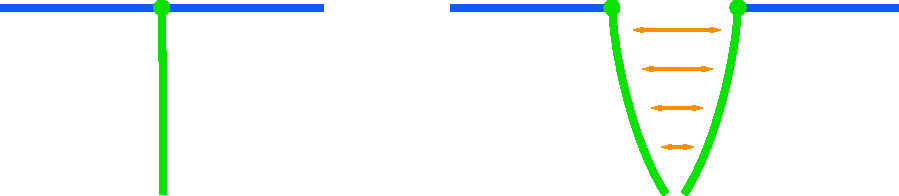
\includegraphics[scale = 0.7]{no_mfld}
\caption{Left: In the brane perspective, the bath CFT on the asymptotic boundary (blue) is connected to two copies of the effective CFT on the brane (green) but the resulting geometry is not a manifold. Right: For excitations below the effective CFT cutoff the system behaves as if it consists of two systems on a manifold which are weakly coupled in the gravitational region (green).}
\label{fig:no_mfld}
\end{figure}

First, we note that constructions where multiple CFTs are joined at a common defect are not rare. For example they appear in the study of boundary and interface CFTs (\eg see \cite{Chiodaroli:2012vc}), and sometimes seem to be required to remove anomalies \cite{Ooguri:2020sua}.

Second, we would like to argue that in the regime where the defect theory can be described by two copies of the boundary CFT coupled to Einstein gravity, we can approximately think of the full theory as two copies of the orbifolded theory (each living on a manifold), which are weakly coupled in the gravitational region -- see the right panel of figure \ref{fig:no_mfld}. This is particularly easy to see from the bulk perspective. For brevity we restrict ourselves to the discussion of graviton modes, but a similar story applies to all bulk fields. 

Let us begin by recalling that for $\veps \ll 1$, the spectrum of graviton fluctuations in the bulk is almost unchanged with respect to the modes in (two copies of) empty AdS space. Hence much of the corresponding physics should be very similar that of two copies of the the AdS$_{d+1}$, or to two copies of the dual CFT$_d$ on the boundaries of two independent AdS$_{d+1}$ geometries. Of course, one exception to the preceding is that upon gluing the two AdS$_{d+1}$ geometries together, a new set of very light graviton states localized in the vicinity of the brane \cite{Randall:1999vf,Randall:1999ee,Karch:2000ct,Karch:2001jb}, as discussed in section \ref{face}. For simplicity, we refer to the latter as the brane graviton modes, while we refer to the former as the standard normalizable modes.\footnote{These bulk modes are $\mathbb Z_2$ graded under reflection across the Planck brane, and the even modes survive the $\mathbb Z_2$ orbifold discussed above include the brane graviton states as well as half of the standard normalizable modes. However, this organization of the modes is not useful for the following discussion.}

On a fixed time slice, as shown in the right panel of figure \ref{fig:brane2}, the standard normalizable modes will describe stress energy excitations in the dual CFT on both the left and right halves of the asymptotic boundary. If we assume an approximate extrapolate dictionary \cite{Harlow:2011ke} for the brane theory as well, these normalizable modes will also describe analogous excitations for the effective CFT on the brane. However, there will be two sets of such excitations: those described by bulk excitations\footnote{We stress here that the localized excitations considered here do not correspond to individual energy eigenmodes, which were implicit in the previous paragraph. Rather they will consist of linear combinations of such eigenmodes evaluated on the fixed time slice being examined here. Of course, having superpositions of energy eigenmodes is what produces the complicated time evolution described below.} with support primarily in the right copy of the AdS$_{d+1}$ geometry, and those described by the analogous excitations primarily in the left AdS$_{d+1}$ geometry. Hence, the stress tensor on the brane can be decomposed into two pieces which correspond to subsectors of the brane theory, each of which is determined by bulk excitations which essentially live on one side of the brane. If these subsectors were truly superselection sectors (\eg as one might imagine arises in the limit $\veps\to0$), our brane theory would contain two independent copies of the boundary CFT  and each of these copies would only interact with the bath CFT on the corresponding half of the asymptotic boundary. That is, each of these systems would live on an independent manifold with topology $S^{d-1} \times \mathbb R$. 

However, this is not strictly correct and the two copies of the CFT on the brane are weakly coupled with $\veps\ll1$ but finite. In particular, localized stress energy excitations of the form considered above will not remain localized with time evolution. Rather they will eventually spread across the entire asymptotic boundary if time evolves for a sufficiently long time. For example, an excitation localized on the right asymptotic boundary will evolve to eventually produce excitations of the stress tensors on the left asymptotic boundary and on the brane as well. From the boundary perspective, excitations moving onto the brane correspond to excitations that are absorbed by the conformal defect (and remain there for a long time).

The spreading of the localized excitations can be seen to arise through two physical effects: First, the bulk excitations can tunnel between the two AdS$_{d+1}$ regions shown in figure \ref{fig:brane2}. Recall that (the radial part of) the linearized bulk equation of motion can be reduced to a Schroedinger equation with a double-well potential, where the height of the barrier is determined by the brane tension \cite{Karch:2000ct}. With $\veps\ll1$ but finite, the barrier height while large remains finite and there will be a finite probability for a bulk excitation on one side of the Planck brane to tunnel to the other. A second independent coupling comes because the stress tensors of the two copies of the CFT couple to the same gravity theory on the brane. From the bulk perspective, the nonlinear Einstein equation produces interactions between the brane graviton modes with excitations on either side of the brane. Hence bulk excitation excitations on one side can leak to the other side by scattering process involving the brane gravitons. However, we note that both effects become smaller as the brane tension approaches its critical value, \ie as $\veps$ approaches zero. Thus, to a good approximation, the brane theory can be treated at two copies of the boundary CFT which only interact weakly. \\


\hd{Entanglement wedge cross-sections:} Recent work \cite{Takayanagi:2017knl,Nguyen:2017yqw} has drawn attention to
the entanglement wedge cross-section, \ie for disconnected boundary regions, the codimension-two surfaces in the bulk which have minimal area and which split the entanglement wedge in two. In particular, there are a number of proposals relating these holographic surfaces to various entanglement measures: entanglement of purification \cite{Takayanagi:2017knl,Nguyen:2017yqw}, reflected entropy \cite{Dutta:2019gen},  odd entanglement entropy \cite{Tamaoka:2018ned,Kusuki:2019evw,Kusuki:2019rbk}, or entanglement negativity \cite{Kudler-Flam:2018qjo,Kusuki:2019zsp}. 

Turning to our model and examining figure \ref{fig:RTPhases}, we see that there are two such minimal surfaces in the connected phase, for which a quantum extremal island appears on the brane. These surfaces are simply disks of radius $P=P_0$ on either side of the brane, with area
\beq\label{reflw}
A=\frac{2\,L^{d-1}\, \Omega_{d-2}}{d-1} \ P_0^{d-1}\, {}_{2}F_1\left[ \frac{1}{2},\frac{d-1}{2},\frac{d+1}{2},-P_0^2 \right]\,,
\eeq
as can be seen from eq.~\reef{A_disc}. The fact that both disks have the same area results from the fact that the corresponding boundary regions are symmetric on either of the conformal defect -- see figure \ref{EEprob}. Of course, if one of the two caps comprising the boundary regions was smaller, the minimal area disk closer to this cap would provide the global minimum and hence become the entanglement wedge cross-section. It would be interesting to understand if the second minimal disk also plays an interesting role in characterizing the entanglement of the boundary state. In this vein, let us add that there are also two additional extremal disks which divide the entanglement wedge in two but their area is actually a local maximum. These disks again lie on either side of the brane but end on $\sigma_\xR$, the intersection of the RT surface with the brane. Again, it is natural to wonder if these surfaces have an interpretation in terms of the boundary entanglement. Let us note that similar surfaces appear in the following discussion.\\

\hd{RT Bubbles and Wormholes:} 

	In appendix \ref{bubble}, we consider a surprising class of RT surfaces with the topology of a sphere, \ie $S^{d-1}$ in the ($d+1$)-dimensional bulk. The appearance of these extremal `bubbles' is quite unusual as they are homologous to the entire boundary. Hence the standard RT prescription would assign an entropy to the ground state of the dual boundary system. Further, presence of a `zero mode' which allows the bubbles to be translated along the brane makes their interpretation even more puzzling. An essential feature for the appearance of the RT bubbles was that the gravitational coupling in the DGP term \reef{newbran} was negative, \ie $\lamb<0$. We also noted that the bubbles do not appear to be macroscopic objects in the brane theory. Rather, as shown in eq.~\reef{haiku2}, their size is always of order of the effective cutoff $\tilde\delta$.
	
Despite the unusual features of these RT bubbles, the discussion in appendix \ref{bubble} highlights a general feature of the quantum extremal islands in a simple way. In particular, as discussed below eq.~\reef{genbubble1}, there are two competing terms contributing to the generalized entropy of these surfaces: the bulk area which describes the entropy of the CFT fields on the brane enclosed by the bubble and the area of the boundary where they intersect the brane, which appears in the gravitational entropy of the DGP term. The bulk contribution naturally acts to contract the bubble but with $\lamb<0$, the brane contribution acts to expand the bubble. As described in the appendix, there is an equilibrium radius where these two effects balance one another. Of course, with $\lamb>0$, the brane contribution also acts to contract the boundary of the bubble and so no closed extremal surfaces appear, as expected.

As noted above, a similar competition is a general feature in the formation of quantum extremal islands. However, in this case as discussed in section \ref{sec:enzyme}, the bulk and brane contributions combine to produce a Bekenstein-Hawking term $\area(\sigma_\xR)/{4G_\mt{eff}}$ on the boundary of the island. This contribution, of course, imposes a large penalty to the formation of a large island and acts to contract the boundary towards a smaller (\ie vanishing) radius. For an island to appear, this contraction must be balanced by an expanding contribution. From the bulk perspective, this is simply coming from the remaining\footnote{We combined part of the bulk area into the Bekenstein-Hawking term above.} bulk area contribution of the RT surface, which we can ascribe to the quantum EE of the CFT state from the brane perspective. The point to be noted here is that for this to provide an expansion the RT surface must be anchored far from the island, \ie in the asymptotic (nongravitational) region associated with the boundary CFT. While perhaps self-evident, this discussion highlights the nonlocal nature of the physics producing the quantum extremal islands.

Let us add that the quantum extremal islands discussed here (as well as the RT bubbles) are remnants of replica wormholes in the limit $n\to1$. This follows from the fact that we are simply studying holographic EE with RT surfaces in a new bulk background, \ie with a back-reacted brane. Hence the analysis of \cite{Lewkowycz:2013nqa}\footnote{Following \cite{Dong:2016hjy,Faulkner:2017vdd}, the same applies for general time dependent situations.} introduces a smooth $n$-fold covering geometry for the corresponding Renyi entropies with positive integer indices. These covering geometries produce smooth wormhole geometries on brane analogous to those discussed in \cite{Almheiri:2019qdq,Penington:2019kki} for two dimensions. 

Now assuming replica symmetry, one can then take a $\mathbb Z_n$ orbifold quotient which leaves a single copy of the boundary geometry but the bulk solution now contains a codimension-two cosmic brane with tension $T_n=(n-1)/(4\Gbk\,n)$. In the presence of a DGP brane, we expect that there is an additional contribution where the two branes intersect, \ie the intersection surface carries an intrinsic tension $\widehat T_n=(n-1)/(4\Gbr\,n)$. In this setting, our discussion above for the formation of quantum extremal islands extends to the Renyi entropies in a relatively straightforward way. In particular, we expect that an area contribution associated with the boundary of the island now carries an effective tension $\tilde T_n=(n-1)/(4G_\mt{eff}\,n)$, which combines the intrinsic tension of this intersection surface and the contribution of the cosmic brane in the vicinity of the Planck brane. The contraction created by this term must be balance by the expansion provided by the remaining cosmic brane contributions. However, to provide an expansion the cosmic brane must be anchored by a twist operator in the asymptotic (nongravitational) boundary. Again, this highlights the nonlocal nature of the physics which implicitly supports the replica wormholes.

Of course, these dynamical considerations are emergent in the topological models considered in \cite{Marolf:2020xie,Penington:2019kki}. Hence it would be interesting to understand the implications of this dynamics to extend the new discussions of baby universes and ensembles to higher dimensions.\\



To conclude, let us comment that we will build on the holographic model constructed here to study the Page curve and the appearance of quantum extremal islands for higher dimensional black holes in \cite{QEI}. In particular, we study eternal black holes coming to equilibrium with an external heat bath (prepared at the same temperature) in a higher dimensional analog of the analysis appearing in \cite{Almheiri:2019yqk}. Let us reiterate that unconventional features (\ie Gauss-Bonnet and DGP couplings) introduced to favour quantum extremal islands here are unimportant in the discussion of higher dimensional black holes.\\





%%% Local Variables:
%%% mode: latex
%%% TeX-master: "../lifeonbrane3"
%%% End:



\bibliographystyle{plainnat}
\bibliography{general-type-theories.bib}

\appendix

\section{Formalisation in Coq}
\label{sec:formalisation-coq}

We have partially formalised our work in the Coq proof assistant~\citep{coq} on top of the HoTT library~\citep{bauer17:_hott}. The formalisation is publicly available at~\citep{lumsdaine:_formal}, wherein further instructions are given on how to compile and use the formalisation.
%
The formalisation will continue to evolve in future; the description here refers to the version tagged as \texttt{\small arXiv}.

The formalisation broadly follows the structure of the paper.
%
\Cref{tab:dict-paper-coq} lists selected major definitions and theorems from the paper, along with the names of the corresponding items in the formalisation, if any.
%
Almost all material of \cref{sec:preliminaries,sec:raw-syntax,sec:typing} has been formalised, as has some but not all of \cref{sec:well-behavedness}.
%
Versions of the main definitions of \cref{sec:well-founded-type-theories} are also formalised, but at time of writing, their treatment in the formalisation has non-trivial differences from the definitions here; such items are marked with an asterisk.
 
\begin{table}[htbp]
  \centering
  \footnotesize
  \begin{tabular}{ll}
    \toprule
    Paper & Formalisation \\ \midrule
    Family
    (\cref{def:family})
    & \coqident{Auxiliary.Family.family}
    \\
%    Family map
%    (\cref{def:family-map})
%    & \coqident{Auxiliary.Family.map}
%    \\
%    Family map over
%    (\cref{def:family-map-over})
%    & \coqident{Auxiliary.Family.over}
%    \\
    Closure rule
    (\cref{def:closure-rule})
    & \coqident{Auxiliary.Closure.rule}
    \\
    Closure system
    (\cref{def:closure-system})
    & \coqident{Auxiliary.Closure.system}
    \\
    Derivation
    (\cref{def:closure-system-derivation})
    & \coqident{Auxiliary.Closure.derivation}
    \\
%    Derivation grafting
%    (\cref{lem:hypotheses-grafting})
%    & \coqident{Auxiliary.Closure.graft}
%    \\
%    Well-founded order
%    (\cref{def:well-founded-order})
%    & \coqident{Auxiliary.WellFounded.well\_founded\_order}
%    \\
    Scope system
    (\cref{def:scope-system})
    & \coqident{Syntax.ScopeSystem.system}
    \\
    De Bruijn scope system
    (\cref{ex:de-bruijn-scope-systems})
    & \coqident{Examples.ScopeSystemExamples.DeBruijn}
    \\
    Syntactic class
    (\cref{def:syntactic-class})
    & \coqident{Syntax.SyntacticClass.class}
    \\
    Arity
    (\cref{def:arity})
    & \coqident{Syntax.Arity.arity}
    \\
    Signature
    (\cref{def:signature})
    & \coqident{Syntax.Signature.signature}
    \\
    Signature map
    (\cref{def:signature-map})
    & \coqident{Syntax.Signature.map}
    \\
    Raw expressions
    (\cref{def:raw-syntax})
    & \coqident{Syntax.Expression.expression}
    \\
    % Renaming action
    % (\cref{renaming-action})
    % & \coqident{Syntax.Expression.rename}
    % \\
    % Signature map action
    % (\cref{def:signature-map-action})
    % & \coqident{Syntax.Expression.rename}
    % \\
%    Renaming functoriality
%    (\cref{prop:commutation-renaming-signature-map})
%    & \coqident{Syntax.Expressions.Renaming}
%    \\
%    Signature map functoriality
%    (\cref{prop:commutation-renaming-signature-map})
%    & \coqident{Syntax.Expressions.Signature\_Maps}
%    \\
    Raw substitution
    (\cref{def:raw-substitution})
    & \coqident{Syntax.Substitution.raw\_substitution}
    \\
    Metavariable extension
    (\cref{def:metavariable-extensions})
    & \coqident{Syntax.Metavariable.extend}
    \\
    Instantiation of syntax
    (\cref{def:instantiation})
    & \coqident{Syntax.Metavariable.instantiate\_expression}
    \\
    Raw context
    (\cref{def:raw-context})
    & \coqident{Typing.Context.raw\_context}
    \\
    Raw rule
    (\cref{def:raw-rule})
    & \coqident{Typing.RawRule.raw\_rule}
    \\
    Instantiation of derivations
    (\cref{cor:instantiation-of-derivations})
    & \coqident{Typing.RawTypeTheory.instantiate\_derivation}
    \\
    Associated closure system
    (\cref{def:associated-closure-system})
    & \coqident{Typing.RawRule.closure\_system}
    \\
    Structural rules
    (\cref{def:structural-rules})
    & \coqident{Typing.StructuralRule.structural\_rule}
    \\
    Congruence rule
    (\cref{def:congruence-rule})
    & \coqident{Typing.RawRule.raw\_congruence\_rule}
    \\
    Raw type theory
    (\cref{def:raw-type-theory})
    & \coqident{Typing.RawTypeTheory.raw\_type\_theory}
    \\
    Acceptable rule
    (\cref{def:acceptable-rule})
    & (not formalised)
    \\
    Acceptable type theory
    (\cref{def:theory-good-properties})
    & \coqident{Metatheorem.Acceptability.acceptable}
    \\
    Presuppositions theorem
    (\cref{thm:presuppositions})
    & \coqident{Metatheorem.Presuppositions.presupposition}
    \\
    Admissibility of renaming
    (\cref{lem:admissibility-renaming})
    & \coqident{Metatheorem.Elimination.rename\_derivation}
    \\
    Admissibility of substitution
    (\cref{lem:admissibility-substitution})
    & \coqident{Metatheorem.Elimination.substitute\_derivation}
    \\
    Admissibility of equality substitution
    (\cref{lem:admissibility-equality-substitution})
    & \coqident{Metatheorem.Elimination.substitute\_equal\_derivation}
    \\
    Elimination of substitution
    (\cref{thm:elimination-substitution})
    & \coqident{Metatheorem.Elimination.elimination}
    \\
    Uniqueness of typing
    (\cref{thm:tight-uniqueness-of-typing})
    & (not formalised)
    \\
    Inversion principle
    (\cref{thm:inversion-principle})
    & (not formalised)
    \\
    Sequential context
    (\cref{def:seq-cxt-by-rules})
    & \coqident{ContextVariants.wf\_context\_derivation}$^{(*)}$
    \\
    Sequential rule
    (\cref{def:sequential-rule})
    & (not formalised)
    \\
    Well-presented rule
    (\cref{def:realisation-well-presented-rule})
    & (not formalised)
    \\
    Well-presented type theory
    (\cref{def:well-presented-type-theory})
    & \coqident{Presented.TypeTheory.type\_theory}$^{(*)}$
    \\
    Well-founded replacement
    (\cref{thm:wf-replacement-equivalence})
    & (not formalised)
    \\ \bottomrule
  \end{tabular}
  \caption{The correspondence between the paper and the formalisation~\citep{lumsdaine:_formal}. Items marked with~$(*)$ differ non-trivially from their counterparts in the paper.}
  \label{tab:dict-paper-coq}
\end{table}

Throughout the paper we worked rigorously but informally, and without discussing which mathematical foundation might be sufficient to carry out the constructions and proofs.
%
On this topic we may consult the formalisation.

Our formalisation is built on top of a homotopy type theory library with an eye towards future formalisation of the categorical semantics of type theories, but is so far agnostic with respect to commitments such as the Univalence axiom or the Uniqueness of identity proofs. The only axiom that we use is function extensionality. In other words, the code can be read in plain Coq.

The formalisation confirms that our development is constructive, there are no uses of excluded middle or the axiom of choice.

It is a bit harder to tell how many universes we have used, because Coq relieves the user from explicit handling of universes. Two seem to be enough, one to serve as a base and another to work with families over the base. The base universe can be very small, say consisting of the decidable finite types, if we limit attention to finitary syntax only.

We rely in many places on the ability to perform inductive constructions and carry out proofs by induction, and so we require some meta-theoretic support for these. Of course, there is no shortage of induction in Coq, and even a fairly weak set theory will have the capability to construct the necessary inductive structures, whereas the higher-order logic of toposes would have to be extended with $W$-types. Alternatively, we could restrict to finitary syntax, contexts and rules throughout to allow Gödelization of 
syntax and reliance on induction supplied by arithmetic.

%%% Local Variables:
%%% mode: latex
%%% End:

% \section{Thirteen ways of looking at a sequential context} \label{app:sequential-context-variants}

TODO This probably wants to remain internal-only, not included in the final submission?

A well-formed context is often defined as something like: a list $A_1, \ldots, A_n$, where for each $i$, $\istype{A_1, \ldots, A_{i}}{A_{i+1}}$.

When formalising this, there are several ways one might make it fully precise.
%
The following are all intended to be reasonable ways of reading the above definition, in a typed metatheory.

The aim here is to look over all such options in excruciatingly fine detail, and convince ourselfs which ones are equivalent, and how trivially/generally.

Most assume our setting of (a) scoped syntax, and (b) using flat raw contexts in the derivability judgemnets.
%
Exceptions are noted.

TODO We could add some more below on how this is affected by (a) unscoped syntax, (b) if the context judgements were mutual with the other judgements, and (c) the “well-formed syntax only” judgement.

\newcommand{\seqcxtlabel}[1]{(\emph{#1}). \label{seqcxt:#1}}
\newcommand{\seqcxtref}[1]{\ref{seqcxt:#1} (\emph{#1})}
\newcommand{\seqrawlabel}[1]{(\emph{#1}). \label{seqraw:#1}}
\newcommand{\seqwflabel}[1]{(\emph{#1}). \label{seqwf:#1}}
\newcommand{\seqrawref}[1]{\ref{seqraw:#1} (\emph{#1})}
\newcommand{\seqwfref}[1]{(\ref{seqwf:#1}) (\emph{#1})}
\newcommand{\seqrawwfref}[2]{\ref{seqraw:#1}(\ref{seqwf:#2}) (\emph{#1}, \emph{#2})}
  
Various ways of defining sequential well-formed contexts from raw flat contexts (without an intermediate stage “sequential raw contexts”):
\begin{enumerate}
\item Seq w-f contexts as an inductive-recursive type, with recursive flattening function \seqcxtlabel{ind-rec}
\item Seq w-f contexts as an inductive-recursive family over $\N$, with recursive flattening \seqcxtlabel{ind-rec-fam}
\item Seq w-f contexts by induction on length, mutual with flattening \seqcxtlabel{ind-by-length}
\item Seq w-f contexts as a (proof-relevant) inductive predicate on raw flat contexts (by the traditional rules) \seqcxtlabel{ind-pred-on-raw}
\item Seq w-f contexts as a list of pairs of a flat context and a well-formed type over it, such that the context of each entry equals the extension of the previous entry’s context by its type \seqcxtlabel{list-pairs}
\item Seq w-f contexts as a vector of types scoped over the length of the vector, such that each type is derivable over the earlier part (in whole scope, i.e.\ no variable-occurrence restrictions) \seqcxtlabel{flat-list-derivable}
\end{enumerate} \saveitem

(To make sense of the “earlier part” in \seqcxtref{flat-list-derivable}, it needs to be read with  a slightly more general idea of flat contexts and derivability: the context is a \emph{partial} map from a scope to types in that scope, and the variable rule has a side condition of definedness.  Or, relatedly, it can be read as working in an unscoped syntax.  The comments below apply to either reading.)

Next, there are various two-stage approaches: a well-formed context is a sequential raw context that is sequentially well-formed, where these are defined as…

\begin{enumerate} \restoreitem
\item seq raw contexts: as inductive type \seqrawlabel{raw-ind-type}
\item seq raw contexts: as inductive family over $\N$ \seqrawlabel{raw-ind-fam}
\item seq raw contexts: defined by induction on length, mutually with flattening \seqrawlabel{raw-ind-length}
\item seq raw contexts: as list of pairs of a scope and type in that scope, such that each scope is the successor of the previous one \seqrawlabel{raw-list-pairs}
\item seq raw contexts: as raw flat contexts of some scope $[n]$, such that the $i$th type is a weakening from scope $[i]$.  \seqrawlabel{raw-list-wkn}
\item seq raw contexts: as raw flat contexts satisfying variable-occurence constraint \seqrawlabel{raw-var-occ}
\end{enumerate}
(Here all except \seqrawref{raw-var-occ} admit a direct definition of the initial segment preceding any entry; for \seqrawref{raw-var-occ} this is non-trivial.)

…followed by:
\begin{enumerate}
\item seq w-f as inductive predicate \seqwflabel{ind-pred}
\item seq w-f by induction on length \seqwflabel{ind-length}
\item seq w-f as non-inductive predicate: each entry is well-formed over preceding initial segment \seqwflabel{non-ind-pred}
\end{enumerate}

(Another axis we could vary, but don’t for now, is proof-(ir)relevance.  All predicates are un-squashed, “derivable” is shorthand for “with a given derivation”.)

So we have $6 + (6 \times 3) = 24$ variants. How equivalent are they?  By equivalent, we always mean “isomorphic, preserving the realisation map to raw flat contexts”.  We assume throughout that the signature is a set, and hence so are expressions, and contexts of any given scope.

\begin{itemize}
\item For direct definitions of sec w-f contexts: \seqcxtref{ind-rec}, \seqcxtref{ind-rec-fam}, \seqcxtref{ind-by-length}, \seqcxtref{ind-pred-on-raw}, and \seqcxtref{list-pairs} are fairly trivially equivalent just by general and fairly standard manipulations of suitable inductive/ind-rec types.

  This leaves \seqcxtref{flat-list-derivable}, which we’ll return to below.
  
\item For seq raw contexts: \seqrawref{raw-ind-type}, \seqrawref{raw-ind-fam}, \seqrawref{raw-ind-length}, \seqrawref{raw-list-pairs}, and \seqrawref{raw-list-wkn} are again fairly trivially equivalent by general facts about inductive types.

  \seqrawref{raw-var-occ} is equivalent to \seqrawref{raw-list-wkn}; but this relies more on specifics of expressions, showing that constraints on variable occurrence are equivalent to being in the image of weakening (which is intuitively clear for renaming along injective scope maps, and I think also true if stated right for renaming along any map).

\item For the seq well-formedness predicate: \seqwfref{ind-pred}, \seqwfref{ind-length}, and \seqwfref{non-ind-pred} are all fairly straightforwardly equivalent.

\item \seqcxtref{ind-by-length} is fairly trivially equivalent to \seqrawwfref{raw-ind-length}{ind-length}.  Along with the above, completes the equivalence of all versions of the definition except \seqcxtref{flat-list-derivable}.

\item \seqcxtref{flat-list-derivable} is \emph{not} necessarily equivalent to the others, for arbitrary raw type theories. But consider type theories satisfying: whenever $\istype{\Gamma}{A}$, then $\istype{\Gamma}{\Gamma_i}$ for each variable $\synvar{i}$ occurring in $A$.  Over such type theories, \seqcxtref{flat-list-derivable} is equivalent to \seqrawwfref{raw-var-occ}{non-ind-pred}.  In particular, any type theory satisfying suitable inversion principles should satisfy this property; we certainly expect any acceptable type theory should satisfy it.  TODO Maybe tight is enough?  It would be nice to prove this, or some metatheorem from which it can be read off!
\end{itemize}

In summary: almost all variants considered here are equivalent for all raw type theories, mostly by (composites/inverses of) fairly general constructions on inductive types.  The exception is \seqcxtref{flat-list-derivable}; this should be equivalent to the others over reasonable type theories, but the equivalence requires a fairly non-trivial metatheorem about derivability.




\end{document}

%%% Local Variables:
%%% mode: latex
%%% TeX-master: t
%%% End:
